%%%%%%%%%%%%%%%%%%%%%%%%%%%%%%%%%%%%%%%%%%%%%%%%%%%%%%%%%%%%%%%%%%%%%%%%%%%%%%%%
%%%%%%%%%%%%%%%%%%%%%%%%%%%%%%%%%%%%%%%%%%%%%%%%%%%%%%%%%%%%%%%%%%%%%%%%%%%%%%%%
%%                           AUTHOR: BIBEKANANDA DATTA                        %%
%%                               (C) MARCH 2024                               %%
%%                      PhD STUDENT, MECHANICAL ENGINEERING                   %%
%%                           JOHNS HOPKINS UNIVERSITY                         %%
%%%%%%%%%%%%%%%%%%%%%%%%%%%%%%%%%%%%%%%%%%%%%%%%%%%%%%%%%%%%%%%%%%%%%%%%%%%%%%%%
%%%%%%%%%%%%%%%%%%%%%%%%%%%%%%%%%%%%%%%%%%%%%%%%%%%%%%%%%%%%%%%%%%%%%%%%%%%%%%%%
%%             PLEASE CHECK THE README.md FILE BEFORE YOU PROCEED             %%
%%              it may be convenient to read this file on GitHub              %%
%%   GitHub: https://github.com/bibekananda-datta/JHU-Dissertation-Template   %%
%% template hosted on this GitHub repository is likely to be the most updated %%
%%%%%%%%%%%%%%%%%%%%%%%%%%%%%%%%%%%%%%%%%%%%%%%%%%%%%%%%%%%%%%%%%%%%%%%%%%%%%%%%

%%%%%%%%%%%%%%%%%%%%%%%%%%%%%%%%%%%%%%%%%%%%%%%%%%%%%%%%%%%%%%%%%%%%%%%%%%%%%%%%
% This is an unofficial dissertation template for Johns Hopkins University.
% As of March 31, 2024, the template follows the dissertation formatting 
% requirements provided by the  Johns Hopkins University Sheridan Library.
% It is the user's responsibility to ensure that the current requirements are 
% followed: https://www.library.jhu.edu/library-services/electronic-theses-dissertations/formatting-requirements/
%%%%%%%%%%%%%%%%%%%%%%%%%%%%%%%%%%%%%%%%%%%%%%%%%%%%%%%%%%%%%%%%%%%%%%%%%%%%%%%%
%%%%%%%%%%%%%%%%%%%%%%%%%%%%%% VERSION HISTORY %%%%%%%%%%%%%%%%%%%%%%%%%%%%%%%%%
% The report class-based template was created by R. Jacob Vogelstein in May 2007
% Updated by Noah J. Cowan on March 01, 2010
% Updated by Brian D. Weitzner on April 29, 2014 
% Updated by John Muschelli on January 29, 2016 
% Updated by Leonardo Collado Torres on April 13, 2016 
% Updated by John Clayton in December 2019
% Last Updated by Bibekananda Datta on March 31, 2024
%%%%%%%%%%%%%%%%%%%%%%%%%%%%%% VERSION HISTORY %%%%%%%%%%%%%%%%%%%%%%%%%%%%%%%%%


%%%% REPORT CLASS with 12 pt font and onesided printing (book class also works)
\documentclass[12pt,letterpaper]{report} 

%%%%%%%%%%%%%%%%%%%%%%%%%%%%%%%%%%%%%%%%%%%%%%%%%%%%%%%%%%%%%%%%%%%%%%%%%%%%%%%%
%% if possible, make your formatting changes here through the variables 
%%%%%%%%%%%%%%%%%%%%%% LIST OF VARIABLES FOR FORMATTING %%%%%%%%%%%%%%%%%%%%%%%%

%%%% JH Library requirement (DO NOT CHANGE)
\def\GlobalMargin{1.0in}                    % margin on all sides
\def\PrintingOffset{0.5in}                  % additional left margin for the printed copy
\def\MainTextSpacing{\doublespacing}        % double-spaced main text


%%%% ADDITIONAL PATHS and FILES
\def\FigurePath{figures}                    % subdirectory for the figure files
\def\BibFileName{thesis.bib}                % name of BibLaTeX-compatible bib file 


\def\FontPackage{lmodern}                   % default font package

\def\HyperlinkColor{blue}                   % color for hyperlinks


%%%% FONT SIZE and TYPESET for DIFFERENT HEADINGS
%% check here for details: https://en.wikibooks.org/wiki/LaTeX/Fonts
%% font format for thesis title
\def\TitleFont{\Large\bfseries\singlespacing\MakeUppercase}  

%% font for chapter, section, subsection, and subsubsection heading
\def\NoSectionLevel{3}                      % 3 levels => section to subsubsection
\def\ChapterFont{\Large\bfseries\singlespacing} 
\def\SectionFont{\large\bfseries\singlespacing} 
\def\SubsectionFont{\normalsize\bfseries\singlespacing}  
\def\SubsubsectionFont{\normalsize\itshape\singlespacing} 


%%%% PARAGRAPH
\def\ParagraphSpacing{\baselineskip}        % spacing between paragraph
\def\ParagraphIndent{0 pt}                  % indentation at the beginning of the paragraph


%% CAPTION
\def\CaptionFontSize{small}                 % caption font size
\def\CaptionLabelFontType{bf}               % boldface label for captions
\def\CaptionSeparator{colon}                % separates caption label from caption text
\def\CaptionSpacing{1.0}                    % single-spaced captions
\def\FigureToCaption{0 pt}                  % spacing between the figure and the caption


%%%% GLOBAL SPACING for TABLES
\def\GlobalTableSpacing{1.5}                % global spacing parameter for table


%%%% HEADER AND FOOTER SETTING
\def\HeaderHeight{30 pt}                    % height of the chapter header
\def\HeaderSpace{12 pt}                     % space between header and the following text

\def\FootnoteSpacing{\baselineskip}         % spacing between footnotes


%%%% BIBLIOGRAPHY ITEMS
\def\BibTextSpacing{\singlespacing}         % single-spaced bibliography
\def\BibItemSpacing{\baselineskip}          % spacing between bibliographic items in reference


%%%% CHAPTER QUOTE (EPIGRAPH PACKAGE)
\def\ChapQuoteFontSize{\small}              % font size of chapter quotes
\def\ChapQuoteLocation{flushright}          % location of chapter quote
\def\ChapQuoteTextShape{\itshape}           % font shape for quotes
\def\ChapQuoteAuthorTextShape{\scshape}     % font shape for quote author
\def\MaxQuoteWidth{0.65\textwidth}          % width epigraph-based quotes in chapter



%%%% SECTION LEVELS and TOC APPEARANCE
\def\NoTOCLevel{2}                          % no of levels showed in the table of contents
\def\TOCIndent{0 pt}                        % indentation in the list of figs and tables
%% 3 levels mean: section to subsubsection.. decrease if you want to show less in TOC


%%%% TOC SPACING of different section levels (chapter to subsubsection)
\def\TOCTextSpacing{\singlespacing}         % single spacing for TOC texts
\def\ChapTOCSpacing{\baselineskip}          % spacing between chapters
\def\SecTOCSpacing{0.5\baselineskip}        % spacing between sections
\def\SubsecTOCSpacing{0.3\baselineskip}     % ... between subsections
\def\SubsubsecTOCSpacing{0.3\baselineskip}  % ... between subsubsections
\def\LOTItemSpacing{\baselineskip}          % spacing between LOT/LOF items



%%%% ADHOC HEIGHT ADJUSTMENT VARIABLES for consistent typesettings
%% following numbers are found by trial and error to compensate 
%% for the default spacing around different LaTeX environments.
%% unless you find inconsistent formatting, you may not need to change these
\def\TitleTopSpacing{-\HeaderHeight-\HeaderSpace}   % top height adjustment for thesis title
\def\BeforeTOCTitleSpacing{-42 pt}          % space before TOC title
\def\AfterTOCTitleSpacing{34 pt}            % space after TOC title
\def\AfterLOTTitleSpacing{34 pt}            % space after LOT/ LOF title

\def\NumChapterTopMargin{-64 pt}            % space before numbered chapter label
\def\UnNumChapterTopMargin{-85 pt}          % space before unnumbered chapter label
\def\ChapLabelToTitle{-27 pt}               % space between chapter label to title 
\def\ChapTitleToText{24 pt}                 % space between the chapter title and the following text
\def\SpaceBeforeQuote{-20 pt}               % white space before quote

%%%% if you want to change any of the heights, adjust using a ruler:
% \usepackage[unit=in,type=upperleftT,color=red,showframe]{fgruler}

%%%%%%%%%%%%%%%%%%%% END LIST OF VARIABLES FOR FORMATTING %%%%%%%%%%%%%%%%%%%%%%


%%%%%%%%%%%%%%%%%%%%%%%%%%%%%%%%%%%%%%%%%%%%%%%%%%%%%%%%%%%%%%%%%%%%%%%%%%%%%%%%
%% add packages as needed but sometimes the order of the packages matters.
%% you may have to change the options of the biblatex package for the bibliography.
%%%%%%%%%%%%%%%%%%%%%%%%%%%%%%% LaTeX PACKAGES %%%%%%%%%%%%%%%%%%%%%%%%%%%%%%%%%

%%%% SOME PRE-REQUISITE PACKAGES
\usepackage[utf8]{inputenc}                 % for encoding input character (required)
\usepackage[american]{babel}                % for different language typography
\usepackage[T1]{fontenc}                    % for font encoding


%%%% DEFAULT FONT (you can specify other fonts - compatibility could be an issue)
\usepackage{\FontPackage}


%%%% COMMON MATH PACKAGES
\usepackage{amsfonts,amssymb,amsmath,amsthm,autobreak,
    cancel,dsfont,mathtools,mathbbol,mathrsfs,siunitx,upgreek}


%%%% TABLE-RELATED PACKAGES
\usepackage{booktabs,longtable,dcolumn,makecell,
    multicol,multirow,tabularx,xltabular,rotating}


%%%% package for micro-typography (you can define more settings)
%% see details here: https://www.khirevich.com/latex/microtype/
\usepackage[activate={true,nocompatibility}]{microtype}



%%%% BIBLIOGRAPHIC PACKAGE (change the style or other options if you need to)
%% Nature style bibliography
\usepackage[backend=biber, defernumbers=true, style=nature, maxnames=99,
     date=year, isbn=false, url=false, doi=true]{biblatex}

%% APA style
% \usepackage[backend=biber, defernumbers=true, style=apa, maxnames=99,
%     isbn=false, url=false, doi=true]{biblatex}

%% IEEE style
% \usepackage[backend=biber,style=ieee,defernumbers=true,maxnames=99, 
%     date=year, isbn=false, url=false, doi=true]{biblatex}



%%%% OTHER PACKAGES AND OPTIONS
\usepackage[pagewise,mathlines]{lineno}     % line numbers for drafting
% \usepackage[ruled]{algorithm2e}             % to manage algorithm environment
\usepackage[titletoc]{appendix}             % to manage appendix chapters
\usepackage{blindtext}                      % to generate random filler texts
\usepackage{calc}                           % to set arithmetic arguments for spacing
\usepackage{caption}                        % to manage captions
\usepackage{comment}                        % to comment a large amount of text as env
\usepackage{epigraph,varwidth}              % for managing quotes
\usepackage{enumitem}                       % to manage list environment
\usepackage{float}                          % to manage floating environment
% footnote environment management
\usepackage[bottom,multiple,hang,flushmargin]{footmisc}      
\usepackage{graphicx,wrapfig}               % to manage images
\usepackage{geometry}                       % to manage margins and page format
\usepackage{glossaries}                     % to add glossaries
\usepackage{fancyhdr}                       % for header/ footer settings
\usepackage[dvipsnames]{xcolor}             % color-related package
\usepackage[a-1b]{pdfx}                     % to generate PDF/A file (add before hyperref)
\usepackage[pdfa]{hyperref}                 % for hyperlink management 
\usepackage[all]{hypcap}                    % for captions on the side of figures
\usepackage{ifthen}                         % if-then statement in LaTeX code
\usepackage{lscape}                         % landscape mode
\usepackage{listings,minted}                % to include codes 
\usepackage{csquotes}                       % yet another package to manage quote
\usepackage{setspace}                       % sets space between lines
\usepackage{seqsplit}                       % splits long character sequence
\usepackage[rightcaption]{sidecap}          % for sideway captions
\usepackage{tocloft}                        % to manage table of contents, etc.
\usepackage{textcomp}                       % text companion fonts in TS1
\usepackage[absolute]{textpos}              % position text at certain location
\usepackage{titlesec}                       % managing different title environments
\usepackage[final]{pdfpages}                % to insert pdf pages
\usepackage{parskip}                        % default spacing around environments
\usepackage{tikz}                           % drawing related package
\usepackage{subcaption}                     % individual panel and caption

%% add more packages and/or change options of the packages as needed
%%%%%%%%%%%%%%%%%%%%%%%%%%%%%% END LaTeX PACKAGES %%%%%%%%%%%%%%%%%%%%%%%%%%%%%
% =e my packages
\usepackage{colortbl}
\usepackage{pifont}% http://ctan.org/pkg/pifont
% \usepackage[labelfont=bf]{caption}
\usepackage{paralist} 

\usepackage{capt-of}% or \usepackage{caption}
\usepackage{graphbox}

\usepackage[noend]{algpseudocode}
% \usepackage[table,xcdraw]{xcolor}
\usepackage{tipa}
\usepackage{xurl}
% \usepackage[fleqn]{amsmath}
\usepackage{placeins}
\usepackage{algorithm}

%%%%%%%%%%%%%%%%%%%%%%%%%%%%%%%%%%%%%%%%%%%%%%%%%%%%%%%%%%%%%%%%%%%%%%%%%%%%%%%
%% specifying direct package options related to document formatting
%%%%%%%%%%%%%%%%%%%%%%%%%%%%%% PACKAGE OPTIONS %%%%%%%%%%%%%%%%%%%%%%%%%%%%%%%%

%%%% GRAPHICX package
\graphicspath{{\FigurePath/}}


%%%% GEOMETRY PACKAGE: margin settings required by JH library 
\geometry{letterpaper, margin=\GlobalMargin, bindingoffset=\PrintingOffset, 
    nomarginpar, includehead, headheight=\HeaderHeight, 
    headsep=\HeaderSpace, includefoot, heightrounded}
%% you can add showframe option to see how the layout looks like


%%%% HYPERREF PACKAGE
\hypersetup{linktocpage, unicode, linktoc=all, colorlinks=true, 
    citecolor=\HyperlinkColor, filecolor=\HyperlinkColor, 
    linkcolor=\HyperlinkColor, urlcolor=\HyperlinkColor}
\urlstyle{rm}           % removes default \texttt style for hyperlinks


%%%% CAPTION PACKAGE
\captionsetup{belowskip=\FigureToCaption, font=\CaptionFontSize, 
    labelfont=\CaptionLabelFontType, labelsep=\CaptionSeparator,
    font={stretch=\CaptionSpacing}, hypcap=true} 


%%%% BIBLATEX: bibliography package settings
\addbibresource{\BibFileName}           % name of the bib file 
% \DeclareFieldFormat{titlecase}{\MakeSentenceCase*{#1}}
\AtBeginBibliography{\urlstyle{rm}}     % roman font family for URL (DOI)
\AtBeginBibliography{\vspace*{8pt}}     % add space for single-spaced bib text

%% the following block ensures articles are sentence case 
%% but the journal names are title case 
\DeclareFieldFormat{sentencecase}{\MakeSentenceCase{#1}}
\renewbibmacro*{title}{%
  \ifthenelse{\iffieldundef{title}\AND\iffieldundef{subtitle}}
    {}
    {\ifthenelse{\ifentrytype{article}\OR\ifentrytype{inbook}%
      \OR\ifentrytype{incollection}\OR\ifentrytype{inproceedings}%
      \OR\ifentrytype{inreference}}
      {\printtext[title]{%
        \printfield[sentencecase]{title}%
        \setunit{\subtitlepunct}%
        \printfield[sentencecase]{subtitle}}}%
      {\printtext[title]{%
        \printfield[titlecase]{title}%
        \setunit{\subtitlepunct}%
        \printfield[titlecase]{subtitle}}}%
     \newunit}%
  \printfield{titleaddon}}


%%%% separate category for papers to be not cited in the bibliography
\DeclareBibliographyCategory{mypapers}             
\newcommand{\mybibexclude}[1]{\addtocategory{mypapers}{#1}}

%%%%%%%%%%%%%%%%%%%%%%%%%%%% END PACKAGE OPTIONS %%%%%%%%%%%%%%%%%%%%%%%%%%%%%%%


%%%%%%%%%%%%%%%%%%%%%%%%%%%%%%%%%%%%%%%%%%%%%%%%%%%%%%%%%%%%%%%%%%%%%%%%%%%%%%%
%% further tweaking variables for the current consistent document formatting
%%%%%%%%%%%%%%%%%%%%%%%%%%%%% DOCUMENT FORMATTING %%%%%%%%%%%%%%%%%%%%%%%%%%%%%%

\setcounter{tocdepth}{\NoTOCLevel}                  % list depth in ToC
\setcounter{secnumdepth}{\NoSectionLevel}           % section to ... subsubsection


%%%% font size and spacing around the titles of ToC/ LoT/ LoF
\renewcommand{\cfttoctitlefont}{\ChapterFont}
\renewcommand{\cftlottitlefont}{\ChapterFont}
\renewcommand{\cftloftitlefont}{\ChapterFont}

\setlength{\cftbeforetoctitleskip}{\BeforeTOCTitleSpacing}
\setlength{\cftbeforelottitleskip}{\BeforeTOCTitleSpacing}
\setlength{\cftbeforeloftitleskip}{\BeforeTOCTitleSpacing}
\setlength{\cftaftertoctitleskip}{\AfterTOCTitleSpacing}
\setlength{\cftafterlottitleskip}{\AfterLOTTitleSpacing}
\setlength{\cftafterloftitleskip}{\AfterLOTTitleSpacing}


%% tweak to TOC to add 'chapter' to the chapter name instead of a number only
%% set the width of the box based on the longest label name
\renewcommand{\cftchappresnum}{\chaptername\space}
\renewcommand{\cftchapleader}{\cftdotfill{\cftdotsep}}  % dots for chapters too
\setlength{\cftchapnumwidth}{\widthof{\textbf{Appendix~XXX~}}}


\setlength{\cftbeforechapskip}{\ChapTOCSpacing}
\setlength{\cftbeforesecskip}{\SecTOCSpacing}
\setlength{\cftbeforesubsecskip}{\SubsecTOCSpacing}
\setlength{\cftbeforesubsubsecskip}{\SubsubsecTOCSpacing}


%% tweak to LOT and LOF to add 'Table'/ 'Figure' to the table/ figure caption listing
%% to change the distance to the start of the table/ figure title
\newcommand*{\noaddvspace}{\renewcommand*{\addvspace}[1]{}}

\setlength{\cfttabindent}{\TOCIndent}               % indentation from tables in LoT
\renewcommand{\cfttabpresnum}{\bfseries Table }
\setlength{\cfttabnumwidth}{\widthof{\textbf{Table~999.999~}}}
\setlength{\cftbeforetabskip}{\LOTItemSpacing}      % spacing between each item
\addtocontents{lot}{\protect\noaddvspace}


\setlength{\cftfigindent}{\TOCIndent}               % indentation from figures in LoF
\renewcommand{\cftfigpresnum}{\bfseries Figure }
\setlength{\cftfignumwidth}{\widthof{\textbf{Figure~999.999~}}}
\setlength{\cftbeforefigskip}{\LOTItemSpacing}      % spacing between each item
\addtocontents{lof}{\protect\noaddvspace}



%%%% TITLESEC: settings for chapter label and title
\titleformat{\chapter}[display]{\ChapterFont}
    {\chaptertitlename\ \thechapter}{\ChapLabelToTitle}{\ChapterFont}

\titlespacing*{\chapter}{0pt}{\NumChapterTopMargin}{\ChapTitleToText} 

\titlespacing*{name=\chapter,numberless}{0pt}{\UnNumChapterTopMargin}
    {\ChapTitleToText}


%%%% TITLESEC: settings for sections, subsection, ... heading format
\titleformat*{\section}{\SectionFont}
\titleformat*{\subsection}{\SubsectionFont}
\titleformat*{\subsubsection}{\SubsubsectionFont}
%% if you had more levels then add settings for paragraph and subparagraph


%% to customize space around section headings, use the following command:
% \titlespacing*{environment-name}{space-left}{space-before}{space-after}


%%%% PARSKIP: for paragraph (and not title) spacing, roughly speaking
\renewcommand{\arraystretch}{\GlobalTableSpacing}   % spacing inside table
\setlength{\parskip}{\ParagraphSpacing}             % paragraph skip
\setlength{\parindent}{\ParagraphIndent}            % paragraph indentation
\setlength{\bibitemsep}{\BibItemSpacing}            % bib item separation 
\setlength{\footnotesep}{\FootnoteSpacing}          % separation between footnote

%%%%%%%%%%%%%%%%%%%%%%%%%%% END DOCUMENT FORMATTING %%%%%%%%%%%%%%%%%%%%%%%%%%%


%%%%%%%%%%%%%%%%%%%%%%%%%%%%% TITLE PAGE MACROS %%%%%%%%%%%%%%%%%%%%%%%%%%%%%%%

\newcommand{\ThesisTitle}[1]{           % prints thesis title
    \vspace*{\TitleTopSpacing}
    {\TitleFont {#1} \par}
}

\newcommand{\ThesisAuthor}[1]{          % prints by ... thesis author in two lines
    by \\ #1 \\
}      

\newcommand{\ThesisStatement}[2]{       % prints thesis or dissertation statement 
    A {#1} submitted to The Johns Hopkins University in conformity \\
    with the requirements for the degree of {#2}
}

\newcommand{\Location}{Baltimore, Maryland}     % prints location

\newcommand{\ThesisDate}[2]{#1 #2}              % prints thesis submission date 

\newcommand{\ThesisCopyright}[2]{               % prints the optional copyright statement
\begin{textblock*}{\textwidth}(\GlobalMargin +\PrintingOffset,9in)
    \copyright\ {#1} {#2} \\ All rights reserved
\end{textblock*}
\null
}

%%%%%%%%%%%%%%%%%%%%%%%%%%% END TITLE PAGE MACROS %%%%%%%%%%%%%%%%%%%%%%%%%%%%%


%%%%%%%%%%%%%%%%%%%%%%%%%%%%%% OTHER MACROS %%%%%%%%%%%%%%%%%%%%%%%%%%%%%%%%%%%

%%%% UNNUMBERED CHAPTERS, SECTION, and SUBSECTION COMMAND for ADDING to TOC
%% removes the 'Chapter #' title while keeping it listed in the TOC
\newcommand\chap[1]{%
    \chapter*{#1}%
    \markboth{#1}{}
    \addcontentsline{toc}{chapter}{#1}}
  
%% removes the 'Section #' title while keeping it listed in the TOC
\newcommand\sect[1]{%
    \phantomsection
    \section*{#1}%
    \addcontentsline{toc}{section}{#1}}
  
%% removes the 'Subsection #' title while keeping it listed in the TOC
\newcommand\subsect[1]{%
    \phantomsection
    \subsection*{#1}%
    \addcontentsline{toc}{subsection}{#1}}

%% removes the 'Subsubsection #' title while keeping it listed in the TOC
\newcommand\subsubsect[1]{%
    \phantomsection
    \subsubsection*{#1}%
    \addcontentsline{toc}{subsubsection}{#1}}

%%%% KEYWORDS for abstract
\newcommand{\keywords}[1]{	
    \textbf{Keywords:} {#1}
}

%%%% TOCLOFT: modified macros/ commands for printing ToC, LoF, LoT
\newcommand{\mytableofcontents}{
    \clearpage
    \renewcommand{\contentsname}{Table of Contents}
    \tableofcontents
    \clearpage
}
%
\newcommand{\mylistoffigures}{
    \clearpage \phantomsection
    \addcontentsline{toc}{chapter}{List of Figures}
    \listoffigures
    \clearpage
}
%
\newcommand{\mylistoftables}{
    \clearpage \phantomsection
    \addcontentsline{toc}{chapter}{List of Tables}
    \listoftables
    \clearpage
}

%%%% IN-TEXT MACROS for own notes (you can define more)
\newcommand{\COMMENT}{\textcolor{red}}
\newcommand{\ADDCITATION}{\COMMENT{(ADD CITATION)}}

%%%%%%%%%%%%%%%%%%%%%%%%%%%% END OTHER MACROS %%%%%%%%%%%%%%%%%%%%%%%%%%%%%%%%%



%%%%%%%%%%%%%%%%%%%%%%%%%%%%%%%%%%%%%%%%%%%%%%%%%%%%%%%%%%%%%%%%%%%%%%%%%%%%%%%
%% only if you plan on using chapter quotes, you may need epigraph settings
%%%%%%%%%%%%%%%%%%%%%%%%%%%%% EPIGRAPH SETTINGS %%%%%%%%%%%%%%%%%%%%%%%%%%%%%%%

\setlength{\epigraphwidth}{\MaxQuoteWidth}              % max width of chapter epigraph
\renewcommand{\epigraphflush}{\ChapQuoteLocation}       % chapter epigraph on right 
\renewcommand{\epigraphsize}{\ChapQuoteFontSize}        % font size for chapter epigraph
\renewcommand{\textflush}{\ChapQuoteLocation}
\renewcommand{\sourceflush}{\ChapQuoteLocation}
\newcommand{\epitextfont}{\ChapQuoteTextShape}          % quote font shape
\newcommand{\episourcefont}{\ChapQuoteAuthorTextShape}  % quote author name shape

%% following settings put variable width underline between quote and author
\makeatletter
\setlength{\beforeepigraphskip}{\SpaceBeforeQuote}
\newsavebox{\epi@textbox}
\newsavebox{\epi@sourcebox}
\newlength\epi@finalwidth
\renewcommand{\epigraph}[2]{%
    \vspace{\beforeepigraphskip}
    {\epigraphsize\begin{\epigraphflush}
    \epi@finalwidth=\z@
    \sbox\epi@textbox{%
        \varwidth{\epigraphwidth}
        \begin{\textflush}\epitextfont#1\end{\textflush}
        \endvarwidth
   }%
    \epi@finalwidth=\wd\epi@textbox
    \sbox\epi@sourcebox{%
        \varwidth{\epigraphwidth}
        \begin{\sourceflush}\episourcefont#2\end{\sourceflush}%
        \endvarwidth
   }%
    \ifdim\wd\epi@sourcebox>\epi@finalwidth 
        \epi@finalwidth=\wd\epi@sourcebox
    \fi
   \leavevmode\vbox{
        \hb@xt@\epi@finalwidth{\hfil\box\epi@textbox}
        \vskip 1ex         % gap between quote and rule
        \hrule height \epigraphrule
        \vskip 1ex         % gap between rule and author
        \hb@xt@\epi@finalwidth{\hfil\box\epi@sourcebox}
   }%
   \end{\epigraphflush}
   \vspace{\afterepigraphskip}}}
\makeatother

%%%%%%%%%%%%%%%%%%%%%%%%%%% END EPIGRAPH SETTINGS %%%%%%%%%%%%%%%%%%%%%%%%%%%%%


%%% define custom settings for other packages here (algorithm/ listing, etc.)

% // =e My macros
\newcommand{\cmark}{{\color{green}\ding{51}}}
\newcommand{\xmark}{{\color{red}\ding{55}}}
\newcommand{\qmark}{{\color{orange}\textbf{?}}}

\newcommand*\blackcircled[1]{\tikz[baseline=(char.base)]{
            \node[shape=circle,fill,inner sep=1.5pt] (char) {\textcolor{white}{#1}};}}


\newcommand{\rulesep}{\unskip\ \color{gray} \vrule\ }

\newcommand{\eg}{{\em e.g., }}
\newcommand{\ie}{{\em i.e., }}
\newcommand{\etc}{{\em etc.}}
\newcommand{\networkname}{Vertigo}
\newcommand{\hostname}{Valinor}
\newcommand{\name}{Vertigo}
\newcommand{\burst}{microburst}
\newcommand{\bursts}{\burst s}


\theoremstyle{definition}
\newtheorem{definition}{Definition}

\newtheorem{theorem}{Theorem}


%%%%%%%%%%%%%%%%%%%%%%%%%%%%%%%%%%%%%%%%%%%%%%%%%%%%%%%%%%%%%%%%%%%%%%%%%%%%%%%
%% these are just some examples; add more settings, macros, environments, etc. 
%%%%%%%%%%%%%%%%%%%%%%%%%%%%%% MATH MACROS %%%%%%%%%%%%%%%%%%%%%%%%%%%%%%%%%%%%

%% basic settings for math environment
\allowdisplaybreaks[1]                  % page break for long equations
\numberwithin{equation}{chapter}        % eqn no with chapter label
\setcounter{MaxMatrixCols}{20}          % no of maximum columns in matrix

%% custom math macros
\newcommand{\dC}{$^{\circ}$C}           % degree celsius symbol
\newcommand{\vect}[1]{\mathbf{#1}}      % boldface for vectors and tensors
\DeclareMathOperator{\T}{{\top}}        % transpose of a matrix/ tensor
\DeclareMathOperator{\tr}{tr}           % trace of a matrix
\DeclareMathOperator{\divg}{div}        % divergence of vector and tensor
\DeclareMathOperator{\grad}{grad}       % gradient of vector and tensor
\DeclareMathOperator{\curl}{curl}       % curl of vector and tensor

%% theorem-style remark environment (custom)
\theoremstyle{definition}
\newtheorem{remark}{Remark}
\counterwithin{remark}{chapter}
%%%%%%%%%%%%%%%%%%%%%%%%%%%%% END MATH MACROS %%%%%%%%%%%%%%%%%%%%%%%%%%%%%%%%%





%%%%%%%%%%%%%%%%%%%%%%%%% DOCUMENT BEGINS HERE %%%%%%%%%%%%%%%%%%%%%%%%%%%

\begin{document}


%%%% TITLE PAGE
%%%% JHU Dissertation title page (if you are not sure, do not change the formatting)

\begin{titlepage}

%% centered single-spaced title page w/o page numbering
\begin{center} \singlespacing \thispagestyle{empty}       


%%%% thesis title: 1.5 inches from the top of the page
\ThesisTitle{Identifying and addressing the implications of bursty network traffic}

\vspace{1in}                    % gap between the title and the author: approx. 1 inch

\ThesisAuthor{Erfan Sharafzadeh}         % author name for the thesis

\vspace{1.5in}                  % gap between the author and statement: 1.5 inches

%%%% for masters, change the arguments to: {thesis}{masters program name}
\ThesisStatement{dissertation}{Doctor of Philosophy}  
%% gap between statement and location: approx. 0.5 inch
\vspace{0.5in} \\               

\Location \\                    % prints Baltimore, Maryland as the location
\ThesisDate{March}{2025}        % thesis submission month and year (single-spaced)


%%%% optional copyright statement: approx. 2 inches from the bottom of the page
%% year and name are input argument for copyright statement
\ThesisCopyright{2025}{Erfan Sharafzadeh}


\end{center}

\end{titlepage}
        

%%%%%%%%%%%%%%%%%%%%%%%%%%%% FRONT MATTER %%%%%%%%%%%%%%%%%%%%%%%%%%%%%%%%

%%%% text spacing, page numbering, and header settings
\MainTextSpacing                            % double spacing for the contents
\pagenumbering{roman}                       % pagination style: Roman numeral
\setcounter{page}{2}                        % page counter starts at roman ii
\pagestyle{fancy}
\renewcommand{\chaptermark}[1]{\markboth{#1}{#1}}
\fancyhead[R]{}               
\fancyhead[L]{\nouppercase \leftmark}       % prints header for unnumbered chap


%%%% MUST ADD ABSTRACT (includes committee as well)
\chap{Abstract} 


Measurements of network traffic unveil periods of high link utilization that can exhaust switch buffers and lead to packet loss. Unfortunately, the diversity and ever-changing nature of networks, whether in a local setting like datacenters or public setting like Internet backbones, workloads and traffic patterns, and even host networking deployments pose a challenge in attributing the sources of bursty traffic in large-scale networks. Additionally, bursts are usually short-lived. Hence, existing proactive countermeasures--e.g., congestion control techniques-- struggle to detect and address them in time. In this study, we first revisit the definition of burstiness in the context of network traffic and introduce a high-resolution network traffic measurement framework, \textit{Valinor},  that employs probes at multiple vantage points to accurately identify and analyze the egress traffic from host machines in order to outline the sources of bursty traffic in host network stacks.

Our findings hint that existing traffic shaping solutions, e.g., packet schedulers, are either ineffective in preventing bursts or do not take into account the bursty nature of the traffic. We demonstrate that Deficit Round Robin (DRR), the de facto fair packet scheduler in the Internet, can perform poorly because of its assumptions about packet size distributions and traffic bursts. Concretely, our study unveils that DRR performs best if (1) packet size distributions are known in advance; its optimal performance depends on tuning a parameter based on the maximum packet, and (2) all bursts are long and create backlogged queues. 
We show that neither of these assumptions holds in today's Internet: packet size distributions are varied and dynamic, complicating the tuning of DRR. Plus, Internet traffic consists of many short, latency-sensitive flows, creating small bursts. These flows can experience high latency under DRR as it serves a potentially large number of flows in a round-robin fashion.
To address these shortcomings, we introduce Self-Clocked Round-Robin Scheduling (SCRR), a parameter-less, low-latency, and scalable packet scheduler that boosts short latency-sensitive flows through careful adjustments to their virtual times without violating their fair share guarantees. 

Finally, we investigate what happens when short-term bursts hit the switch buffers at the core of the network and packet loss becomes imminent. We introduce selective packet deflection, a reactive measure to prevent microbursts from causing expensive packet drops in the event of extreme buffer congestion. Packet deflection aims to use the available buffer in neighboring switches in managed environments to temporarily host packets that arrive at full buffers, significantly reducing the packet loss and improving application performance.

Burstiness remains an important aspect of network traffic as technologies and workloads evolve. We hope that this study paves the way for periodically revisiting this phenomenon in order to design burst tolerant networks.

%% list of keywords seperated by comma
\keywords{Traffic Bursts, Datacenter Networks, Host Networking, Packet Scheduling, Packet Deflection}


%%%%  committee members (add it right after the abstract w/o page break)
\begin{singlespace}

    %% if you have co-advisor, add here w/ \vspace{0.1in} as shown below
    %% alternatively you can use minipage environment to put side-by-side
    \section*{Primary reader and thesis advisor}
    
    Dr. Soudeh Ghorbani \\
    Assistant Professor\\
    Department of Computer Science\\
    Johns Hopkins University, Baltimore MD 


    \section*{Secondary readers}
    
    Dr. Yair Amir\\
    Professor Emeritus\\
    Department of Computer Science \\
    Johns Hopkins University, Baltimore, MD 
    
    \vspace{0.1in}
    
    Dr. John Ousterhout \\
    Professor\\
    Department of Computer Science \\
    Stanford University, Stanford, CA 

    \vspace{0.1in}
    
    Dr. Alex Marder \\
    Assistant Professor\\
    Department of Computer Science \\
    Johns Hopkins University, Baltimore, MD 

    %% you can add more readers if you have them on your committee 
    %% use \vspace{0.1in} in between members for clarity
    %% you can also place committee members side-by-side using `minipage`


\end{singlespace}


%%%% OPTIONAL but COMMON: preface chapters
%%%% did not use \chap command because the chapter does not have any name
% \chapter*{~}
% \addcontentsline{toc}{chapter}{Dedication}


% %%%% there is no format for this page (sample is shown, you can do as you like)
% \begin{center}                  % horizontally centered text
% \vspace*{3in}                   % adjust the spacing to center it vertically
%     \begin{onehalfspacing}      % tighter spacing for multi-line statements
%     \textit{
%     Dedicated to those who fight for freedom\\
%     and those who lost their lives fighting for freedom
%     }
% \end{onehalfspacing}
% \end{center}
\chap{Acknowledgment}

This dissertation would not have been possible without the guidance, help, and support of the following people.

First and foremost, I'd like to sincerely thank my Ph.D. advisor Dr. Soudeh Ghorbani for her insights and support throughout this journey. Under her guidance, I learned to be an independent researcher, and to effectively shape and present my research. I am forever grateful for this opportunity.

I'd like to thank Jean Tourrilhes who patiently mentored me during my internship at Hewlett Packard Labs. I learned a ton and more from him!

I'd like to thank my Master's degree advisor Dr. Mohsen Sharifi who taught me how to think about the philosophy of designing systems.

I'd like to thank all my co-authors. None of this has been possible without their help. I thank Dr. Puneet Sharma at Hewlett Packard Labs. There is nothing that can't happen with his unlimited support.
I sincerely thank Dr. Showan Asyabi and Dr. Alireza Sanaee. I started my research journey with them and have been ever asking for their insights. I thank my dear friend Sepehr Abdous for all his help and being there in all deadline crunches!
I thank Dr. Timothy Zhu and Raymond Matson. I learned a lot from them.
I thank the current and previous members of the Foundational Networked Systems Lab and the Network and Distributed Systems Lab at HPE for their feedback and support.

I'd like to recognize my Graduate Board and Thesis committee for their insights and comments on my research. I thank Dr. Yair Amir for the deep conversations that shaped my thinking when I started my Ph.D at Johns Hopkins. I thank Dr. John Ousterhout for the opportunity to help improve Homa implementation through rigorous measurement and experimentation.
I thank Dr. Alex Marder for the opportunity to help with the Computer Networks course along with all the advice on entering the job market. I thank Dr. Gianni Antichi for his warm and helpful comments on my research. I thank Dr. Ryan Huang for teaching me invaluable insights on the history and evolution of system software design. I thank Dr. Tamas Budavari for his comments and insights on earlier versions of my research.

Finally, I'd like to thank my family. My mom, dad, and my partner for their love and support. I am forever indebted to them.        
\chapter*{~}
\addcontentsline{toc}{chapter}{Epigraph}

%% it is a less common optional page with no specific requirement

\begin{center}                      % horizontal centering of the texts
\vspace*{2.5in}                     % adjust the space to place vertically centered
\begin{onehalfspacing}
    \textit{
    Hacking means exploring the limits of what is possible, \\ in a spirit of playful cleverness. \\
    Activities that display playful cleverness have "hack value".
    } \\
    
    \rule{1.5in}{0.5pt} \\          % length and thickness of the rule
    
    \textsc{-- Richard Stallman}
\end{onehalfspacing}
\end{center}
%% you can have other chapters and the order does not matter


%%%% LISTINGS
\TOCTextSpacing                             % single spacing for the table of contents
\microtypesetup{protrusion=false}           % turn off protrusion from microtype
\hypersetup{linkcolor=black}                % local black hyperlink for TOC
%
\mytableofcontents                          % MUST
%
\mylistoftables                             % MUST: if you have tables
%
\mylistoffigures                            % MUST: if you have figures
%
%% OPTIONAL: you can add more lists here (but you will have to define those)
%
\hypersetup{linkcolor=blue}                 % revert it back to blue
\microtypesetup{protrusion=true}            % turn on protrusion from microtype

%%%%%%%%%%%%%%%%%%%%%%%%%%% END FRONT MATTER %%%%%%%%%%%%%%%%%%%%%%%%%%%%


%%%%%%%%%%%%%%%%%%%%%%%%%%%%% MAIN MATTER %%%%%%%%%%%%%%%%%%%%%%%%%%%%%%%

%%%% PAGE and TEXT settings 
\MainTextSpacing                        % restores double spacing 
\pagenumbering{arabic}                  % Arabic page numbering
\fancyhead[L]{\chaptername\ \thechapter. \nouppercase \leftmark}


%%%% include all the main text chapters
\chapter{Hacking Traffic Bursts: An Introduction} \label{chap:chap-1}

% if you want a short header you can use the following command
% \chapter[short-header-name]{chapter-title} \label{chap:chap-1}

Measurement studies show that traffic is bursty across a wide range of timescales in diverse contexts such as Ethernet LANs \cite{selfsim}, WANs \cite{wan}, data centers \cite{fbIMC22}, and WWW traffic \cite{web}.
In particular, microsecond-scale congestion events, sometimes called \emph{microbursts}, have been the focus of numerous measurement and control papers recently \cite{swift, conquest, snappy, radar, high-resolution, wild, fbIMC22,incast}. However, the modulating effect of host networking on traffic burstiness at various timescales is relatively less investigated. This study starts by addressing this gap.
We ask \emph{what causes the traffic to emerge from hosts in bursts?} Is burstiness an \emph{scale-invariant} property of traffic, i.e., does the traffic retain its burstiness across a wide range of timescales, or do the microbursts become smooth at coarse timescales? Are canonical burst countermeasures such as TCP pacing and packet scheduling effective in curtailing bursts?

These questions have far-reaching implications for network performance and design. Controlling bursts at different timescales requires deploying mechanisms that operate at the corresponding pace. Microbursts, for instance, require real-time techniques with sub-RTT control loops, whereas bursts at longer timescales can be more effectively managed by resource provisioning techniques such as topology engineering and routing that take seconds to minutes to complete \cite{gemini}.

Unfortunately, studying the impact of host networking on bursts is complex. Take the Linux network stack as an example: the egress traffic that originates from the Linux kernel stack passes through many layers and optimizations before arriving at the wire. Transport protocol internals like initial window size, cumulative acknowledgments, queueing disciplines (qdiscs), driver rings, segmentation offloading, and hardware packet scheduler at the NIC all handle the traffic.
All these elements and their complex interactions can play a role in forming or suppressing bursts at various timescales. 
%
These challenges are further compounded by the heterogeneity, scale, and 
the velocity of evolution in today's networks that constantly change in response to increasing demand and the rollout of new services \cite{snap, evolvable, govindan2016evolve}. 

\section{Contribution I: Measuring the Burstiness}

We build \textit{Valinor} \cite{valinor}, a high-resolution traffic measurement framework that enables network operators to systematically and periodically dissect the elements of host networking, their impact on traffic burstiness in isolation, and importantly, their interactions with the emergent traffic patterns, all at different timescales. To ensure visibility into the impact of the software stack and the shape of the traffic on the wire through time, \textit{Valinor} is composed of two main components: 1) An in-host timestamping framework (\textit{Valinor-H}) based on \textit{eBPF} that collects egress packet metadata nearly at the last stage of software stack processing. 2) An in-network packet timestamping framework (\textit{Valinor-N}) that captures packet arrival timestamps in the programmable switch data plane immediately after the NIC, and sends the timestamp data to offline servers for collection, storage, and burstiness analysis. 

Our analysis of the impact of host networking on the shape of traffic using \textit{Valinor} reveals some surprising results. 
% different contexts
As an example, classical work paints a unifying and consistent picture of scale-invariant burstiness, i.e, they show the same degree of variability across a wide range of timescales in a variety of different network types \cite{selfsim, wan, web}.
% 2: app-layer
It has also been established that this scale-invariant burstiness is primarily caused by \emph{application layer} characteristics such as long-tailed flow size distributions and is ``robust'': it holds for a variety of transport protocols (e.g., TCP Reno, Vegas, and flow controlled UDP) and various network configurations \cite{filesize, feldmann1999dynamics}.

In contrast, our investigations paint a more nuanced and complex picture. We show that burstiness at various timescales varies significantly across host configurations (hardware configurations, transport protocols, scheduling, etc.). We also show the pronounced modulating effect of below application layer elements on bursts. This implies that, for the same heavy-tailed flow size distribution, the ultimate shape of traffic on the wire depends heavily on the host configuration such as the NIC scheduler. Plus, \textit{Valinor}'s analysis of newer reliable transport protocols (e.g., Homa \cite{homa}, DCTCP \cite{dctcp}, and BBR \cite{bbr}) reveals the high degree of variability of burstiness for these protocols. As an example, BBR is less bursty not just at fine timescales (a result that is consistent with the literature \cite{homa, homa-impl}) but also at coarse timescales. The latter finding (new to the best of our knowledge) implies that techniques such as topology engineering \cite{gemini} and multi-timescale congestion control \cite{mts_cc}---premised on the long-range burstiness of traffic---may yield limited performance improvements under these new protocols. 

Finally, given the impact of some variants of transport protocols on bursts, we quantify the effectiveness of TCP pacing and active queue management paradigms such as CoDel \cite{codel} in qdiscs (software packet schedulers) in mitigating bursts. 
%
Our results show the pronounced impact of lower-layer functions (residing in the driver and NIC) on forming the ultimate shape of traffic on the wire relative to the higher-layer software operations of the TCP/IP stack and qdiscs. 
As an example, active queue management techniques such as CoDel and RED in the Linux kernel try to prevent the formation of large and lasting bursts. However, our results show that their impact is effectively erased by offloading (TCP Segmentation Offloading (TSO), serialization, etc.) and the NIC scheduler. 
For example, while in isolation, the frequency of large 300 kB bursts under CoDel is 500 times lower than FIFO, this difference is barely visible on the wire after packets pass through the multi-queue NIC with segmentation offloading.
Moreover, TCP pacing enforced in the qdiscs generates between 1.8$\times$-19$\times$ larger bursts when NIC scheduler and offloading are in action compared to when in isolation.\footnote{Despite making the traffic bursty and hard to manage, these low-level functions are essential for reducing the processing overhead and meeting the increasingly high link rates. For example, disabling TCP segmentation offload results in a 3$\times$ increase in CPU utilization, 71\% lower throughput, and a 46\% increase in median packet RTTs for a multi-flow \textit{Iperf} test. 
Relatedly, disabling MQ results in a 4\% decline in the throughput of the same workload.
} 
This result indicates that the countermeasures for controlling bursts should be moved further down the packet processing pipeline at the end hosts. 

Our results on the variability of burstiness (based on hardware configurations, transports, etc.)---combined with the ever-evolving workloads and features in today's networks---highlight the need for periodic traffic measurement and analysis. 
In chapter \ref{chap:chapter-2}, we introduce the mathematical notions developed for capturing bursts across time, present their practical implications in networks (\S\ref{sec:valinor-background}), provide some background on host networking and the design space of burst measurement frameworks (\S\ref{sec:valinor-space}), and present the design of Valinor (\S\ref{sec:valinor}) before delving into our findings (\S\ref{sec:valinor-findings}).

% ========================================
\section{Contribution II: Revisiting Fair Packet Scheduling}

The Internet is continuously evolving as a multi-party environment. To meet service performance requirements, enforcing isolation at different levels ranging from tenants to applications and individual flows is crucial \cite{sharing,loom,carousel,fairnic,mrfq,heracles}. 
% To this end, cloud providers and network operators employ a variety of solutions, including packet scheduling, to ensure that different workloads meet their quality of service demands within their resource utilization budget \cite{arachne,snap,ghost,syrup,caladan,drr,loom,aifo}.
Packet scheduling offers an opportunity to enforce fine-grained
control over network bandwidth both at the edge and core of the
network. Despite the abundance of scheduling techniques that rely on explicit labeling, such as strict priority queues \cite{aifo,karuna,afq} or time wheels \cite{carousel,calendar}, obtaining flow priorities or timestamps from
Internet transports is usually not feasible.
% and managing QoS across the Internet is an open problem.
Instead, Fair Queuing provides fine-grained fairness without flow information, and has been deeply studied from fairness, latency bounds, and computational complexity standpoints
\cite{gps,wfq,nagle,scfq,stfq,wf2q}. Since Fair Queuing schedulers suffer from non-linear computational complexity which hinders their deployment \cite{stfq,scfq,wf2q}, a middle-ground alternative is to
use Deficit Round-Robin (DRR) scheduling 
% or one of its derivatives 
because of its low overhead and scalability \cite{drr,aliquem,strr,frr}. Indeed, DRR is used everywhere from hardware traffic
management pipelines to software middleboxes, host stacks, and network interface cards 
\cite{loom,cisco,juniper,tc,pifo,intel710,intel810}.

Regrettably, the nature of the Internet traffic since Deficit Round-Robin was proposed has changed, and the drawbacks of DRR are increasingly problematic.
Workloads such as realtime video conferencing and voice communication, streaming, cloud gaming, and instant messaging have become widespread among more traditional web and file transfer \cite{rtc,pandemic,video,zoom,confucius,gaming,enterprise,baidu,canyousee}. Such workloads feature a diverse set of properties concerning flow counts, flow arrival rates, flow sizes, packet lengths, packet inter-arrivals, and burstiness \cite{cachelib,enterprise,milisampler,baidu,wild,autosens,canyousee}.
First, concerning burstiness, Internet traffic traces feature bursts of packets with diverse lengths and inter-arrivals \cite{caida, mawi,ccdc,wild,im}. Long bursts are more prone to create backlogged queues at the packet scheduler, while, broadly, short bursts belonging to latency-sensitive applications such as web and streaming  \cite{edge,passive} exhibit periodic on-off arrivals. For example, the
median response size for web workloads does not exceed 10 kB, while
Variable Bit-Rate (VBR) streaming workloads such as Zoom have
a median frame length of 10 kB with large idle gaps between frames
\cite{passive}.

Our experiments with DRR reveal that under
a backlogged scheduler, a bursty latency-sensitive flow has to wait
for up to a full scheduling round, i.e., until all the flows have been
serviced at least once, to be able to send its traffic. This can be
detrimental to the performance of such flows, resulting in much higher application latency compared to Fair Queueing Schedulers. 
Even with recent enhancements to DRR such as Sparse Flow Optimization (SFO) \cite{sfo}, which prioritize new incoming flows from backlogged flows to improve responsiveness, bursts with more than one packet are prone to being quickly demoted to lower-priority and having to compete with backlogged flows, thus experiencing long delays.

Secondly, packet lengths are diverse and skewed \cite{caida,
mawi,ccdc,wild,im,harmony} and packet length distribution for
wide-area network traffic is difficult to generalize. Many modern
applications use small packets to reduce latency and the impact of
packet loss \cite{webrtc-teams, zoom-quality}. Network Interface
hardware acceleration \cite{linux-gso-gro} may produce very large
packets (64 kB).
DRR relies on a fixed, user-specified quantum equal to (or higher
than) the maximum packet size in the network \cite{drr}, making it
hard to tune. Configuring DRR with a conservatively large quantum can
be detrimental to  intermediate buffers as it allows the scheduler
to send large bursts of packets when servicing each flow
\cite{strr,aliquem}, ultimately causing increased response times for
latency-sensitive applications.
\textit{No packet scheduler today can offer low resource utilization,
low latency, and adaptability to packet sizes without explicit flow information feedback.}

Our work makes several novel contributions to the fair scheduling domain.
First, we show that the drawbacks of DRR, i.e., high latency for bursty flows and
vulnerability to quantum choice, are measurable at the application
level, even on high speed networks. We further identify the
trade-off between latency and CPU utilization as an inherent part of
DRR's design and argue that there is no correct answer to configuring
DRR (\S\ref{sec:scrr-background}).

Second, we formally outline the design of Self-Clocked Round-Robin
(\textit{SCRR}) \cite{scrr}, a novel multi-queue round robin scheduler. \textit{SCRR}
borrows virtual clocking from Fair Queuing \cite{stfq,scfq} to eliminate the quantum and enforce fairness, and services sub-queues like DRR in
strict sequence for simplicity and scalability. As a result, \textit{SCRR} is
parameter-less, light, scalable, and adapts to both bursts and
packet length variations in the network. We design various \textit{SCRR}
enhancements to efficiently prioritize bursty flows, in order to
reduce the application latency.
When an idle  flow becomes active, the scheduler must decide its bandwidth allowance through its virtual clock setting. 
Backed by strong theoretical virtual clocking principles, \textit{SCRR} can efficiently adjust the virtual clocks for short, bursty flows to allow them to quickly make progress without violating the scheduler's fairness bounds (\S\ref{sec:scrr-design}).
Third, we provide rigorous proof of flow burstiness and fairness for
\textit{SCRR}. Precise virtual time accounting guarantees
that \textit{SCRR} has the same fairness as DRR with a low maximum burstiness bound (\S\ref{sec:scrr-analysis}).

Fourth, we evaluate \textit{SCRR} and competing schedulers on a physical testbed under Cubic and BBRv3 
using novel experiments. Application-level
fairness is tested with thousands of active TCP flows while application latency is measured for request-response flows and VBR traffic.
Our results demonstrate that employing \textit{SCRR} as a software switch
results in 23\% lower CPU utilization compared to DRR with 1500B
quantum. Our results further reveal that \textit{SCRR} offers 93$\times$, 71\%,
and 45\% lower response times over tail-drop, DRR with a small
quantum, and DRR with a large quantum,
respectively. (\S\ref{sec:scrr-evaluation})

\textit{SCRR} is a step toward more dynamic packet scheduling for multi-party
wide-area deployments. \textit{SCRR} is the first true alternative to DRR, it
offers the low latency of Start Time Fair Queuing with the low
complexity of DRR. Our ultimate goal is for \textit{SCRR} to replace existing
hardware and software packet schedulers because of its plug-and-play
deployment, low resource consumption, low scheduling latency, 
desirable fairness, and compatibility with bursty workloads.

% ========================================
\section{Contribution III: In-situ Reactions to Bursts}

% Driven primarily by two trends---the disaggregation of storage, compute, and memory across the network for cost savings and the rising demand for high-speed transmission in new technologies and applications \cite{swift, hpcc}---datacenters today have exceedingly stringent low-latency requirements. To enable resource disaggregation, remote resources (GPU, memory, disk, etc.) should be accessible over the network within 3-5$\mu s$ \cite{hpcc}. In emerging applications and technologies such as NVMe (non-volatile memory express) and large-scale machine learning workloads, the network is frequently the performance bottleneck because their storage and computation resources are extremely fast \cite{hpcc}. Despite significant progress towards building ultra-low-latency datacenter networks in recent years, why does the network continue to remain the performance bottleneck? A key challenge is reportedly \emph{microbursts}, short-lived periods of congestion that last for less than a millisecond and cause the majority of packet loss in datacenters \cite{wild, high-resolution, hpcc}. The extreme packet drops caused by \bursts \ lead to re-transmissions that impose significant latency and degrade application performance. 
% People talking about mbursts are citing random papers: From DCTCP to TLP to the recent ToN paper
%
Managing \bursts \ is challenging because of their short lifespans and their diverse and ever-changing root causes (applications, TCP artifacts such as ACK compression, offloading features in NICs, \etc \ \cite{high-resolution, bullet, measuring, dctcp, why, notes,ipbursts, coalescing, snap,valinor}). 
%Even measuring \bursts \ poses technical challenges. 
Rack-level traffic measurements at Facebook, for instance, show that more than 70\% of \bursts \ last for less than a few tens of microseconds, significantly shorter than the frequency of most deployed measurement frameworks \cite{high-resolution}. More recent studies confirm the prevalence of incast traffic patterns, where a large number of hosts simultaneously transmit data to a single receiver, in large-scale datacenters \cite{swift,milisampler,incast}.

% numerous studies have tried, at the edge and in the core. A large number of recent proposals try to manage \bursts \ at hosts and in the network core. 
Given the necessity of reacting to \bursts \ in situ and in real-time, a group of proposals attempts to manage \bursts \ in the network core, \eg via  balancing the load among multiple shortest paths \cite{drill}, deflecting the excess load across neighboring switches with spare capacity \cite{dibs, pabo}, and provisioning enough buffer space in switches to absorb bursts \cite{bufferFacebook}. Although effective for small scales and lightly loaded networks, network-centric techniques fail under load and at scale. Load balancing and buffer sizing techniques, for example, cannot manage large-scale incasts because the intensity of the burst in such cases exceeds the buffer capacity of any single datacenter switch (commonly shallow buffered) and the number of paths that the burst can be distributed among. Similarly, deflecting packets extends their path lengths, \eg by 20\% under 50\% offered load ($\S$\ref{sec:deflection}), and increases utilization which exacerbates the congestion if the network is already overloaded. By preventing packet drops, deflection further delays informing the hosts that they need to throttle their send rate. Our experiments show that under 80\% load, random deflection completes $10\times$ fewer incast queries and the average flow completion times is $45\%$ higher than a simple baseline. 
%Plus, packet deflection leads to excessive packet reordering that is detrimental to transport protocols and applications. 
Datacenters today experience a wide range of workloads, scale, and utilization, including frequent epochs of high utilization and extreme-scale incast events (thousands of flows arriving simultaneously at the same destination) \cite{nature, swift, hpcc}. For a burst management technique to be viable, it is an essential necessity that it handles extreme load gracefully.

On the other hand, given the greater visibility and control over the sources of traffic at the edge, another group of host-centric designs strives to proactively identify and prevent the formation of \bursts \ at the edge, sometimes with some feedback from the network (\eg regarding the queueing delay \cite{hpcc} and congestion \cite{dctcp}). Adding jitter in the application layer to prevent synchrony \cite{jitter}, credit-based transport protocols that coordinate and schedule the flows sent to a receiver \cite{pHost, NDP, homa}, and feedback-based congestion control protocols that strive to impede bursts and their subsequent packet loss by reacting to increasing RTTs and network congestion faster \cite{dctcp, SECN, hpcc, swift} are all examples of designs in which the hosts play a central role in preventing the formation of \bursts. Compared to core-centric designs, host-based techniques are fundamentally limited by their slower reaction to \bursts, typically an RTT or slower.
%

We advocate co-designing the networking layer in the core and the edge to make it burst-tolerant. Given that \bursts \ are extremely short-lived, the network core should be capable of handling them in real-time and in place, \eg by distributing microburst packets across the network. However, to remain efficient under various degrees of load, the network should distinguish between \bursts \ and an overall high degree of load and treat each differently. For example, while \emph{deflecting} the packets of a local, transient burst to other switches when the overall utilization is low improves flow completion times, \emph{dropping} them, when the overall load is high, helps reduce the congestion and improves performance. Making such distinctions can be greatly facilitated with some assistance from the edge. We show that a simple and efficient extension to senders' networking stack enables such discretion in the network core by tagging packets with flow size information. Similarly, on the receiver-side, a re-sequencing shim layer can retrieve the correct ordering of packets and thus shield the transport and application protocols from the excessive reordering caused by deflection.

To realize this vision, we design \textit{Vertigo} \cite{vertigo}, an edge-core co-design of the networking layer that leverages end-host knowledge of the flow size information to selectively deflect and drop packets based on their likely contribution to persistent congestion (as opposed to \bursts). \textit{Vertigo} consists of three components deployed on the path of a datacenter packet. (1) We design an extension to the end-hosts network stack that tracks and tags every packet inside a flow with the remaining bytes of its flow, referred to as RFS (Remaining Flow Size)\footnote{
In \S\ref{sec:eval}, we show that \textit{Vertigo} continues to be more effective than other baselines such as ECMP and DIBS \cite{dibs} even when flow size information is not available in advance. However, having this information improves its average incast query completion time by 13\%.
% In \S\ref{sec:eval}, we show that Vertigo continues to be more effective than the state-of-the-art such as DRILL \cite{drill} even when RFS is not available in advance. However, having this information improves its performance by 12\%.
}. A boosting module decreases the RFS fields of re-transmitted packets to ensure they do not starve. 
%Combined with mechanisms to detect packet re-transmissions, Vertigo is able to improve the completion of bursty flows. 
 (2) In the network core, when a switch receives a packet and the output queue of the packet is full, the switch selects the packet with the largest RFS among the newly arrived packet and the packets in its output queue to deflect:
%\ie to detour to a neighboring switch that is not necessarily on a packet's shortest path towards its destination. To deflect this packet, t
the switch then randomly selects two queues and inserts the packet into
% to 
the least loaded one. If both queues are full, the switch randomly selects one of them and drops the packet with the largest RFS among the enqueued packets and the deflected packet in order to keep the packets with the lowest RFS in the queue. (3) Finally, we design a transport-independent packet ordering framework on the receiver hosts' RX path that detects and buffers out-of-order packets to wait for packets experiencing prolonged RTTs due to deflection.
%. the intuition behind distinguishing mbursts and lasting congestion
Packets of the flows with more bytes 
% of
to send (\ie those with large RFS) are more likely to contribute to persistent congestion. When facing \bursts, Vertigo prioritizes such packets for deflecting (when a randomly selected queue in the switch has spare capacity) and for dropping (when the network is congested, indicated by two randomly selected queues being \emph{both} full at the same time). This enables \textit{Vertigo} to gracefully handle \bursts\  even under extreme loads.

\textit{Vertigo} is a burst-tolerant, fast L2/L3 routing technique for datacenters. Albeit more efficient than its L2/L3 counterparts, it still only provides a best-effort reachability service that may drop and reorder packets. Thus, it should be deployed below the appropriate transport protocols that provide higher-level services such as congestion control (\eg to throttle the send rate when the overall send rate is higher than the capacity of the network), loss recovery (due to congestion and failures), and fairness. In our evaluations, we test the performance of \textit{Vertigo} as the substrate running below TCP, DCTCP, and a state-of-the-art datacenter congestion control algorithm, Swift \cite{swift}. \textit{Vertigo} consistently outperforms the other L2/L3 baselines such as DIBS \cite{dibs} (a representative of deflection routing in datacenters), DRILL \cite{drill} (a microburst-tolerant load balancer), and ECMP (the most widely deployed forwarding protocol in datacenters) for all these transport protocols, especially under load and extreme incast scales. For example, in a network with 55\% overall link utilization and a bursty workload, \textit{Vertigo}+DCTCP reduces mean incast query completion times (QCT) by 48\%, and 58\% over DRILL+DCTCP and DIBS+DCTCP, respectively. Under 85\% load, incast queries finish 47\% and 68\% faster under \textit{Vertigo}+DCTCP compared to DRILL+DCTCP and DIBS+DCTCP. Under the same load (85\%), \textit{Vertigo}+Swift improves the QCT of DRILL+Swift and DIBS+Swift by a factor of 32 and 15, respectively.

At its core, \textit{Vertigo} is a deflection routing technique that harnesses hosts' visibility into the workload to remain efficient under extreme scales and loads. We demonstrate why a naive implementation of deflection quickly fails in typical datacenter scenarios (\S\ref{sec:deflection}), outline our design for making deflection practical in datacenters (\S\ref{sec:v2}), and evaluate the effectiveness of Vertigo in typical datacenter scenarios, including under various degrees of load, traffic burstiness, and two datacenter topologies, via extensive simulations and microbenchmarks (\S\ref{sec:eval}).

This thesis scratches the surface of burstiness, its definitions, implications, and design considerations.
We reiterate the importance of studying the network traffic burstiness at different timescales. We design and implement \textit{Valinor} a high-resolution measurement framework using programmable network capabilities in host network stacks and the switching fabric and identified the inefficacy of software-based measures inside the hosts in preventing burstiness. Our results further call for rethinking the design of existing traffic shaping mechanisms such as packet schedulers with traffic characteristics in mind. To this end, we target the Deficit Round-Robin (DRR) scheduler, a most popular fair packet scheduling paradigm for both software and hardware deployments, and identify several assumptions in DRR's design that remain incompatible with the dynamic and bursty nature of the Internet traffic today. We then propose Self-Clocked Round-Robin (SCRR), a novel scheduling paradigm for low-latency, high-throughput, and low burstiness. Finally, to address short-term bursts that overwhelm network buffers, we introduce selective packet deflection, a novel realtime reaction mechanism to packet loss in datacenter networks.

These contributions, when combined together, help realize burst-tolerant networks. However, the process of designing a fully burst-tolerant network would outlive this study. Each individual networking component is susceptible in creating bursts or performing poorly when facing bursty traffic. Moreover, the workload dynamics in both local networks and wide-area networks constantly change. Therefore, periodic measurements is a must to ensure that our networks are resilient against bursts. Finally, while packet deflection proves a strong solution to recover from the destructive impact of microbursts, more work is required to make it practical, efficient, and compatible with existing deployments (\S\ref{chap:chap-6}).
\chapter{Understanding the Impact of Host Networking Elements on Traffic Bursts} \label{chap:chapter-2}

%%%% OPTIONAL EPIGRAPH EXAMPLE
% \epigraph{What we have to learn to do, we learn by doing.}{-- Aristotle}


%%%% MUST: if the chapter is a reprint or submitted paper, you must declare it
%% you can use enumerate or itemize environment if you have more than one paper 
%% \mybibexclude{} will exclude this citation from the final bibliography
%% if this paper appears somewhere else then remove \mybibexclude{} command

% \begin{singlespace}         % you can also use `onehalfspace` to relax the spacing
%     This chapter is adapted from the following article with permission from <publisher>
    
%     \fullcite{einstein}. \mybibexclude{einstein}
% \end{singlespace} 
% \vspace{-3mm}
\section{Background: scale-invariant burstiness}
\label{sec:valinor-background}
% \vspace{-2mm}
Measurements of the Internet traffic show periods of sustained greater-than-average or lower-than-average traffic rates across a wide range of timescales \cite{wan,web,vbr,selfsim,filesize}. 
%
This behavior, sometimes called \emph{scaling} or \emph{self-similarity}, has broad implications for performance. In this section, we first formalize the notion of self-similarity and re-introduce the Hurst exponent, a mathematical representation of self-similarity, before discussing the implications of self-similarity and characterizing bursts at fine timescales such as microbursts.

\paragraph{Self-similarity.} 
Self-similarity is a notion pioneered by Benoit Mandelbrot \cite{mandelbrot} which refers to a phenomenon where a certain property of an object (such as an image or a timeseries) is preserved with respect to scaling in space and/or time. If an object is self-similar, its parts, when magnified, resemble the shape of the whole \cite{self_similar_overview}.

More formally, let $(X_t)_{t\in \mathbb{Z_+}}$ be a timeseries, e.g., this timeseries can represent a traffic trace measured at some fixed time granularity. The aggregated series $X^{(m)}_i$ is defined as 
\[X^{(m)}_i=1/m(X_{im-m+1}+...+X_{im})\]
In other words, $X_t$ is partitioned into blocks of size $m$, their values are averaged, and $i$ denotes the index of these blocks. 
%

\emph{Autocorrelation} is a mathematical representation of the degree of similarity between a timeseries $X_t$ and a time-shifted version of $X_t$ over successive time intervals. It measures the relationship between the current value of a timeseries and its future values.
A strong positive autocorrelation for a traffic volume timeseries, for example, suggests that if the volume is high (i.e., higher than average) now, then it is likely to be also high in the next time slot, whereas a strong negative autocorrelation implies that a high-volume slot is likely to be followed by a low volume one.

Let $r(k)$ and $r^{(m)}(k)$ denote, respectively, the autocorrelation functions (ACFs) of $X_t$ and $X^{(m)}_i$ where $k$ is the time shift from the original timeseries. We say that $X_t$ is \emph{self-similar}, or more accurately \emph{asymptotically second-order self-similar}, if these conditions hold: 
\begin{align}
r(k) \sim c \times k^{-\beta}\\
r^{(m)}(k) \sim r(k)
\end{align}

\noindent for large $k$ and $m$, where $0<\beta<1$ and $c$ is a constant, and $f(x)\sim g(x)$ as $x\to a$ means that $\lim_{x\to a} f(x)/g(x)=1$ \cite{mts_cc}. $X_t$ is self-similar in the sense that its ACF $r(k)$ behaves hyperbolically with $\sum^\infty_{k=0}r(k)=\infty$ (Eq. 1). This property is also referred to as \emph{long-range dependence}. Equation 2 implies that for self-similar timeseries, the autocorrelation structure is preserved with respect to time aggregation.

In networks, the traffic is called self-similar if the aggregated traffic over varying timescales remains bursty, regardless of the granularity of the timescale.

\paragraph{The Hurst exponent.} Let $H=1-\beta/2.$ $H$ is called the \emph{Hurst exponent.} The Hurst exponent, a number in the $(0,1)$ range that is sometimes referred to as the \emph{index of long-range dependence}, is a measure of the long-term memory of a timeseries. It characterizes the self-similarity and long-range dependence of the timeseries: 
\begin{compactitem}
\item{\underline{$0.5<H<1$} indicates a self-similar timeseries with long-term positive autocorrelations, i.e, a high value in the series (e.g., higher than average traffic volume) is likely to be followed by another high value. Plus, the values a long time into the future also tends to be high.

It follows from Eq. (1) above that the closer $H$ is to 1, the more long-range dependent $X_t$ is. Conversely, $H$ values closer to 0.5 show weaker long-range dependence.
}
%
\item{\underline{$H=0.5$} indicates a completely uncorrelated series.}
%
\item{\underline{$0<H<0.5$} indicates a \emph{mean-reverting} timeseries, i.e., one with long-term switching between high and low values in adjacent pairs of time slots. That is, a single high value in the timeseries is likely to be followed by a low value.\footnote{Note that the $0<\beta<1$ condition in the equations above is a requirement for self-similar, and not mean-reverting, series.}
}
\end{compactitem}

Various techniques (e.g., rescaled-range analysis and Periodogram \cite{hurst-comp}) exist for estimating $H$ for an empirical dataset. Similar to the seminal work on Bellcore Ethernet traffic self-similarity \cite{selfsim}, we use the rescaled-range, \emph{R/S}, for the results presented in this paper. The details of this method are presented in Appendix \S\ref{app:rs}.

\begin{figure}[t]
    \centering
    \begin{subfigure}[t]{0.38\linewidth}
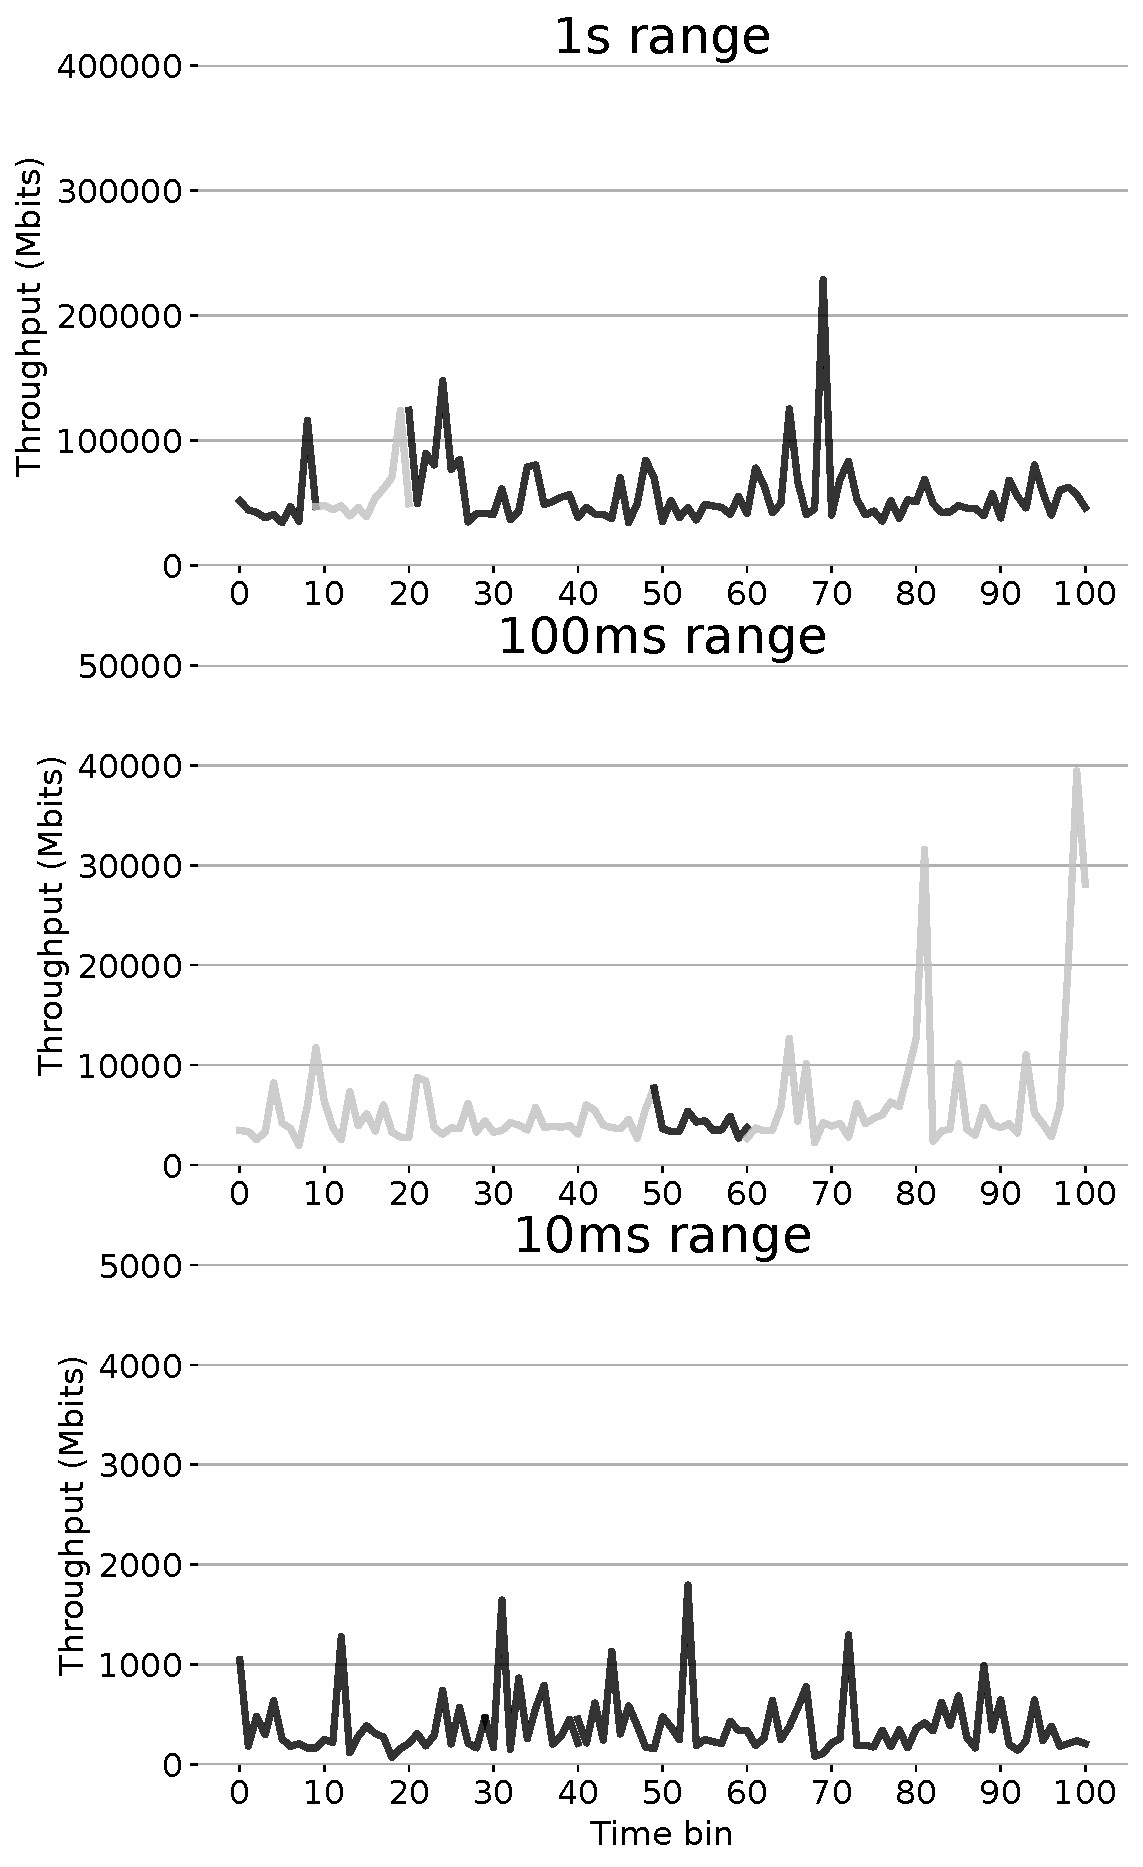
\includegraphics[width=1\linewidth]{figs/self_similarity.pdf}
    \caption{\textbf{Time-series}}
	\label{fig:self-sim}
\end{subfigure}
    \begin{subfigure}[t]{0.33\linewidth}
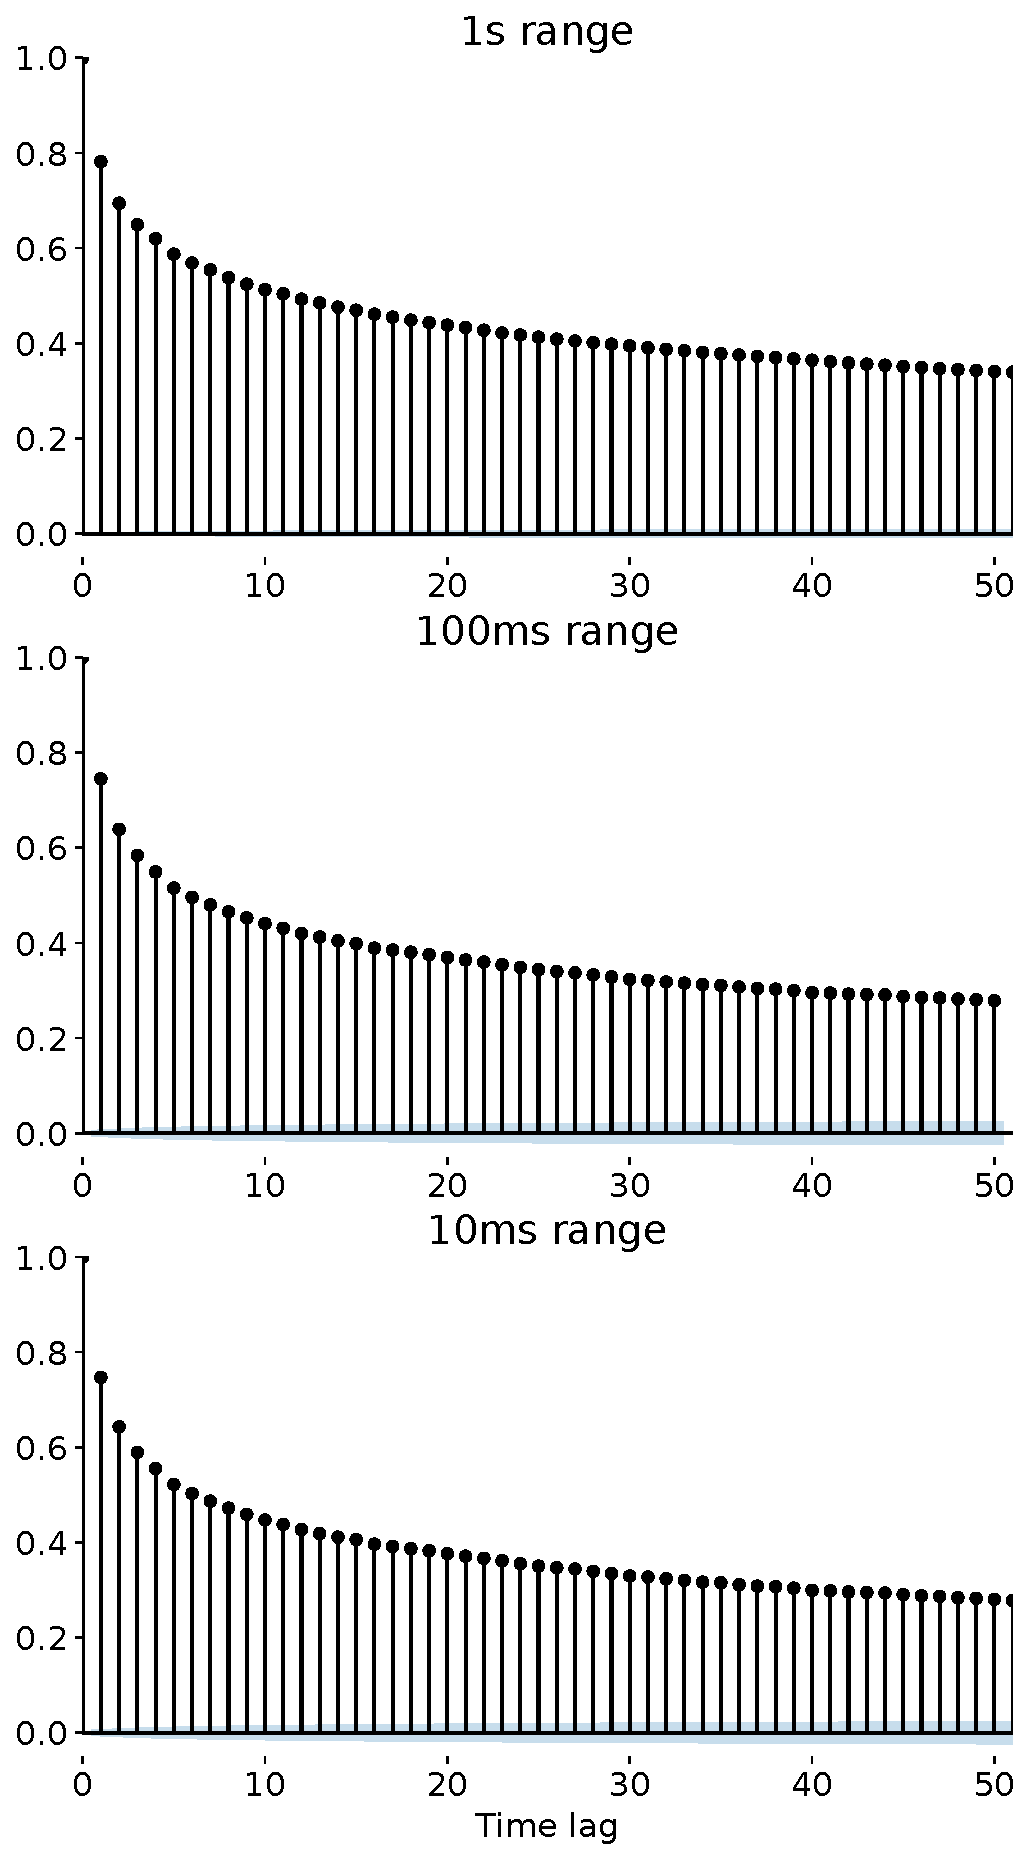
\includegraphics[width=1\linewidth]{figs/acf.pdf}
    \caption{\textbf{Auto-correlation}}
	\label{fig:autocor}
\end{subfigure}
 % \vspace{-3mm}
    \caption{\small{A self-similar timeseries with H=0.88.}}

\label{fig:motiv}
 \vspace{-2mm}
\end{figure}

\paragraph{Example:} Figure \ref{fig:self-sim} (the first row) shows a simulated scenario where 32 TCP connections generate a synthetic workload using Pareto flow size distribution with a mean of 4200 kB and $\alpha=1.05$ and exponential arrivals that create 6 Gbps offered load.
We plot the traffic rate (in Mbps) against time where time granularity is 1$s$. A data point is the aggregated traffic volume over a $10 ms$ interval. The second row of the same figure depicts the same traffic series where a randomly selected second interval in the first timeseries (the highlighted segment in the first row) is magnified by a factor of ten, resulting in a granularity of $100 ms$ in the truncated timeseries. The last row similarly rescales a randomly selected slot by 10$\times$. The figures show that this trace is self-similar: when traffic is aggregated over varying timescales, the aggregate traffic pattern remains bursty, regardless of the granularity of the timescale. 
%
This visual scaling is confirmed by the Hurst coefficient, $H=0.88$, and the autocorrelation functions of the trace (Figure \ref{fig:autocor}) that show positive, slow (almost polynomial) decaying, and consistently shaped correlations across various timescales. Slow-decaying ACFs signify long-range dependence in a timeseries.

\paragraph{Practical implications of self-similarity.}
Self-similarity has broad implications on network design and performance, e.g., it is shown to lead to increased delay and loss \cite{filesize, mts_cc, adas1995resource, addie1995fractal, duffield1995large, likhanov1995analysis, norros1994storage}. We next discuss some of the key implications of self-similarity: 

\begin{compactitem}
\item{\textbf{Queueing performance and buffer sizing.} Self-similarity greatly influences queueing performance. From a queueing theory standpoint, the defining characteristic of self-similarity is that the queue length distribution decays much more slowly than short-range-dependent traffic (polynomially vs. exponentially under short-range dependent traffic, e.g., Poisson processes) \cite{mts_cc}. For strongly self-similar traffic, the mean queue length increases with the buffer size \cite{park1997effect}. This implies that  networks with strongly self-similar traffic should deploy small buffers to control the queueing delay. }

\item{\textbf{Throughput and latency trade-off.} Prior work \cite{filesize, park1997effect} shows that jointly provisioning low delay and high throughput is adversely affected by self-similarity.}

\item {\textbf{Traffic prediction and burst countermeasures.} The correlation structures present in self-similar traffic can be detected and exploited to predict future traffic over timescales larger than an RTT \cite{mts_cc}.\footnote{The prediction methods span diverse domains such as regression theory, neural networks, and estimation theory \cite{mts_cc}.} Traffic prediction at long timescales, in turn, is invaluable for designing the appropriate burst countermeasures. For instance, resource provisioning techniques with control loops larger than an RTT (e.g., multi-scale congestion control \cite{mts_cc}, re-routing, and topology rewiring \cite{gemini}) enhance the performance of self-similar traffic.}

\end{compactitem}


\paragraph{Microbursts.} Given their ubiquity and impact, in particular in data centers, microsecond-scale traffic surges, known as \emph{microbursts}  \cite{wild,hpcc,high-resolution}, have been the focus of many recent proposals \cite{conquest,vertigo,acc,swift,bfc,hpcc}.

The intensity of a microburst has often been measured implicitly based on buffer utilization, or in more extreme cases, packet loss. Related work also quantifies microbursts as the number of packets from one flow that occupy a buffer at a time snapshot \cite{radar}, the evolution of switch queue length over time \cite{observation}, an uninterrupted sequence of packets with gaps of smaller than a threshold \cite{bullet}, and/or sequence size of larger than a threshold \cite{bs}.
Using metrics that are independent of network queues allows us to perform universal measurements in the entire network, i.e., both at the hosts and the switches. Yet, measurement systems intending to quantify microbursts can leverage all the above definitions to provide a holistic view of burstiness behavior.

From the technical perspective, we define a burst as the cumulative sum of packet bytes whose inter-arrivals are smaller than a threshold $\tau$. Setting the minimum value for $\tau$ initially depends on link speeds and MTUs. For example, in a fully utilized 40 Gbps link with MTU = 1500 bytes, packets arrive 300 ns apart. Therefore, an initial $\tau$ of 2-10$\times$ of this value is small enough to detect microbursts and large enough not to miss consecutive packets from flows. To ensure that $\tau$ is not affected by the network configuration and the internal characteristics of the workloads, we repeat our measurement with a wide range of values for $\tau$.


\section{Approaches to measuring traffic bursts}
\label{sec:valinor-space}
%In order to explore the design space for capturing packet arrivals, it is worthwhile to first review the path of the packets in the network stack.
In this section, we provide a brief background on host networking and present the design space of burst measurement frameworks before discussing Valinor in \S\ref{sec:valinor}.

\begin{figure}
    \centering
    	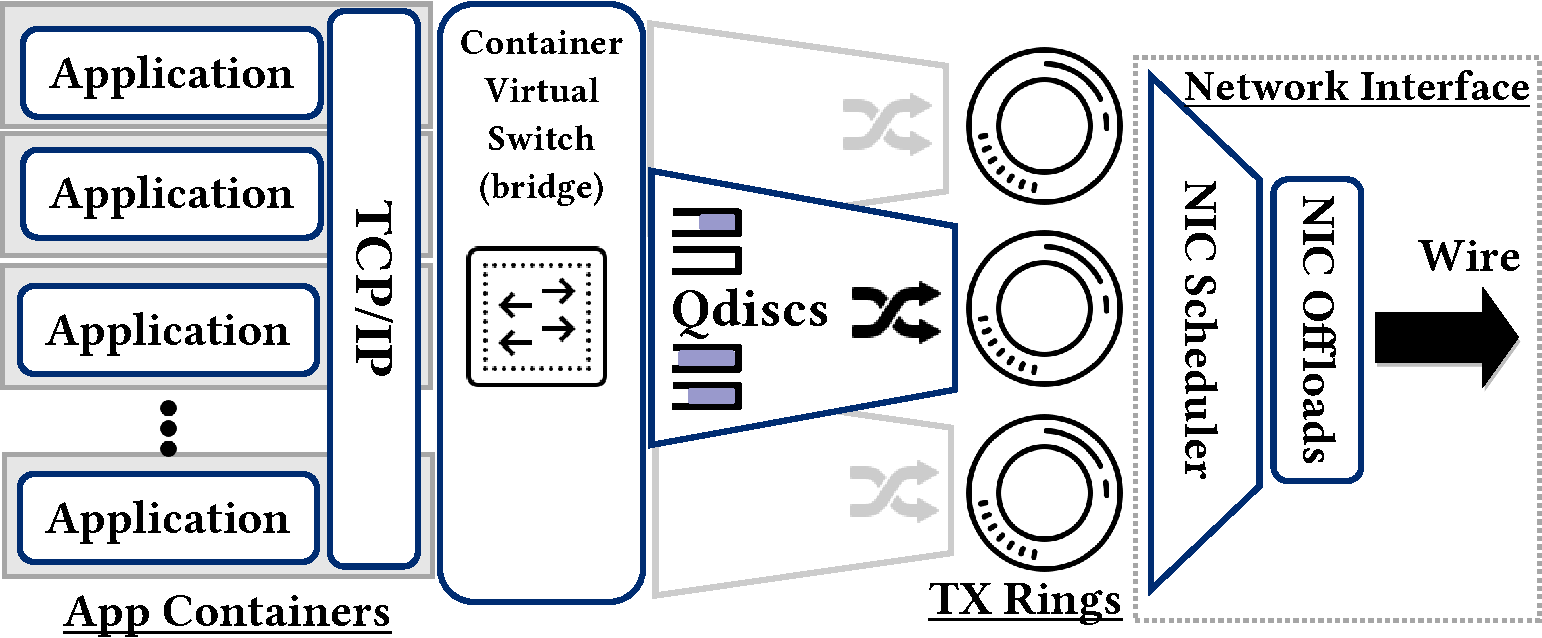
\includegraphics[width=0.80\linewidth]{figs/hostack-crop.pdf}
    	% \vspace{-2mm}
    \caption{\small{Conventional network processing stack architecture in a containerized Linux deployment.}}
    \vspace{-2mm}
	\label{fig:hostack}
	    \vspace{-3mm}
\end{figure}

\subsection{Conventional host networking}
Conventional network stacks consist of various processing layers glued together via several optimization techniques. In Linux, application data is passed to socket interfaces (buffering in the userspace), and then to the transport protocol processing (transport buffers, short queues \cite{tsq}). Transport protocols populate \textit{sk\_buffs},\footnote{\textit{sk\_buff} stands for "Socket buffer" and is used to represent the socket data that eventually is shaped into the packet. \textit{sk\_buffs}, therefore, may contain a single or multiple packets.} a collection of data pointers and  header information. After performing routing, \textit{sk\_buffs} eventually make their way towards interface \textit{qdiscs}, the hierarchical packet schedulers in Linux. \textit{qdiscs} operate in parallel on all CPU cores and forward the scheduled \textit{sk\_buffs} towards driver rings where another layer of buffering is performed before notifying the NIC \cite{titan}. Finally, with the conventional offloading features enabled, the NIC performs scatter/gather \cite{breakfast}, segmentation, checksum, and sends the packets on the wire \cite{overheads}. Figure \ref{fig:hostack} depicts an overview of the packet's path through the network processing pipeline in a Linux host.

% \subsection{Designing a measurement framework: challenges and trade-offs}
% Figure \ref{fig:timestamp} depicts potential means of capturing timestamps to measure traffic burstiness during packet transmission.
% \begin{table*}[t]
% \resizebox{\textwidth}{!}{%

% \begin{tabular}{l|c|c|c|c|c|c|c|c|c}
% \rowcolor[HTML]{dfe9f8} 
% \multicolumn{1}{c|}{Method} & \multicolumn{1}{c|}{Latency}  & \multicolumn{1}{c|}{Throughput}  & \multicolumn{1}{c|}{CPU utilization}    & \multicolumn{1}{c|}{Interference}   & \multicolumn{1}{c|}{Scalability}          & \multicolumn{1}{c|}{Granularity}  & \multicolumn{1}{c|}{Data analysis} & \multicolumn{1}{c|}{Intermediate layer capture} & \multicolumn{1}{c}{Wire traffic capture}  \\ \hline \hline
% % \rowcolor[HTML]{fbe5d6} 
% In-network timestamping  & \cmark & \cmark & \cmark & \cmark & \cmark & Packets & Offline & \xmark & \cmark \\ \hline
% \rowcolor[HTML]{dfe9f8} 
% eBPF timestamping on TX path     & \xmark & \xmark & \xmark & \xmark & \cmark & sk\_buffs & Offline & \cmark & \xmark \\ \hline
% % \rowcolor[HTML]{fbe5d6} 
% Commodity NIC timestamps        & \cmark & \cmark & \xmark & \xmark & \xmark & sk\_buffs & Offline & \cmark & \xmark  \\ \hline
% \rowcolor[HTML]{dfe9f8} 
% Programmable NIC timestamps & \qmark & \qmark & \qmark & \cmark & \cmark & Packets & Offline/Online & \qmark & \qmark \\ 
% \end{tabular}
% }
% \vspace{-3mm}
%   \caption{\small{\textbf{Different approaches to capturing packet arrivals. Checks (\cmark) represent the utility of the proposed solution. Crosses (\xmark) represent the shortcomings, and the question marks (\qmark) demonstrate inconsistency in available features. In-network timestamping provides a zero-overhead and scalable way to monitor traffic burstiness but lacks visibility into host stack intermediate layers. eBPF data planes provide better visibility into qdiscs and transport protocol's traffic shape but suffer from software overheads.}}}
% %   \vspace{-0.8cm}
% \vspace{-5mm}
%   \label{tab:techniques}
% \end{table*}

\subsection{Capturing timestamps}

High-resolution timestamping is essential for burst analysis. Various techniques exist for capturing packet arrivals:
\\
\\
\textbf{NIC timestamps.}
Hardware timestamping is available in all commodity NICs. This feature  is supported by the Linux kernel via ancillary socket data. When a user requests timestamping through a socket option, the transmission timestamps are generated in the hardware before sending the packet on the wire and are eventually sent to the source socket. Therefore, the application is responsible for polling the error queue and reading the timestamps.
Hardware timestamping supports most TCP and UDP connections, however, it suffers from two main shortcomings.
First, if the operating system fails to poll the timestamp registers of the NIC in time, e.g., in higher packet rates, the timestamp will be overwritten by that of the next packet.
Plus, modifying the network application to receive timestamps may impact the application's workload pattern, and thus must be performed with extra care.
\\
\textbf{Modifying networking stack software.}
To study realistic network traffic with higher arrival rates, hardware timestamping is not ideal due to the need to change the application internals and high overheads. An alternative solution is to directly capture the timestamps closer to the packet processing, e.g., the NIC driver, and either add the timestamps to the packet payload or re-route them to the userspace. Alas, accessing and modifying the packet data requires offloading features such as scatter-gather IO and Segmentation Offloading to be turned off. Additionally, timestamps that are at \textit{sk\_buff} granularity may not imitate the inter-packet gaps on the wire due to the intervention of lower layers.
\\
\\
\textbf{eBPF hooks.}
eBPF offers a series of hooks inside the Linux kernel and the NIC driver that allows fast execution of arbitrary data plane logic. An eBPF program consists of a data plane and a control-plane code targeting a specific hook on the RX or TX path (XDP hook in the receive path of NIC driver and traffic control (\textit{tc}) hook on the TX path of the qdisc subsystem are two examples). eBPF \textit{tc} programs are registered to the kernel using the \textit{tc} command and are executed inside a lightweight RISC virtual machine. eBPF also provides fast data structures that enable shared state between the kernel and the userspace. This allows us to perform burst measurements offline with any workload configuration without modifying the kernel source or packet payloads.

While eBPF relieves us from directly modifying the packet processing code in the kernel, it presents two shortcomings. First, eBPF, similar to the previous solution, works at \textit{sk\_buff} granularity since packet segmentation is almost always offloaded to the NIC. Therefore, the eBPF framework can only measure the gaps between larger chunks of data, not packets. Additionally, our measurements show that each eBPF invocation incurs  up to 1 $\mu$s of delay, mostly due to memory accesses. While this overhead may be acceptable at the \textit{sk\_buff} granularity, the framework will lose its visibility into nanosecond-scale events. Ultimately, eBPF provides a convenient solution to plug into the network data path with minor interference. Making it a viable burstiness probing point on the egress path. We present the design and implementation of the Valinor eBPF framework, Valinor-H, in \S\ref{sec:host}.
\\
\\
\textbf{Timestamping in the switch data-plane.}
A holistic method to capture the behavior of all host networking components (including the NIC) is to perform measurements immediately after transmitting the packets on the wire, i.e., at the first network hop. Fortunately, the rise of programmable switch architectures with high-resolution timestamping enables capturing packet arrival timestamps and sending this data off the critical communication path for offline processing.
This further ensures zero interference with the ongoing communication and the ability to track the entire egress host networking components. We describe the design of our in-network measurement system, Valinor-N, in \S\ref{sec:innetwork}. 
\\
\\
% Table \ref{tab:techniques} summarizes the advantages and disadvantages of using the above techniques for timestamping. eBPF timestamping does not require any modifications to the kernel or the application--unlike commodity NIC timestamps--but suffers from slight performance degradation due to the additional imposed latency. The added latency is further amortized when breaking a large sk\_buffs to smaller MTUs. In-network timestamping allows fast accurate acquisition of telemetry data that is sent to offline servers for processing.
\textbf{Programmable NICs} share many of the strengths of in-network measurements (e.g., timestamping close to the wire, low overhead, and no interference) but do not provide visibility into in-network queue occupancies. Plus, our experience with commodity DPUs \cite{dpu} shows inconsistencies in the capabilities of existing devices. General-purpose SoC NICs \cite{dpu} are either bound to their slow ARM CPUs or do not offer per-packet timestamping capabilities on their fast path. Due to these practical issues as well as the greater visibility that in-network measurements offer, alongside its host module, Valinor currently leverages programmable networks for capturing bursts on the wire.

% Finally, with the rise of programmable network interfaces, we envision that they can eventually embrace in-host traffic measurement frameworks. Our initial experience in trying to implement a traffic measurement framework in commodity DPUs \cite{dpu} reveals that existing devices are not consistent in their capabilities. General-purpose SoC NICs \cite{dpu} are either bound to their slow ARM CPUs or do not offer per-packet timestamping capabilities on their fast path. On the other hand, a full design and implementation of a traffic measurement framework on an FPGA-based NIC is beyond the scope of this study, yet a viable future direction that can combine the visibility of in-network frameworks with the scalability of in-host alternatives.

\section{Valinor measurement framework}
\label{sec:valinor}

For designing Valinor, we have three goals in mind:
\begin{compactenum}
    \item Offering visibility into the host networking traffic, as well as the shape of the traffic on the wire.
    \item Offering high-resolution timestamping of packet arrivals in line with the increasing link bandwidths and faster packet processing pipelines.
    \item Providing insights on traffic shape and burstiness at different scales and time ranges.
\end{compactenum}

We design and implement Valinor, a measurement framework that consists of two main timestamping prongs to study packet arrivals from the host and network vantage points.
First, we design Valinor-H to study the host's view of its egress traffic by choosing \textit{tc} eBPF hooks. For capturing the external picture of traffic burstiness, we design Valinor-N, a timestamping module for programmable fabric.

\subsection{Valinor-H: burst measurement in hosts}
\label{sec:host}
% Capturing packet departures in the host network stack requires direct visibility into the kernel. eBPF offers a series of hooks inside the Linux kernel and the NIC driver that allows fast execution of arbitrary data plane logic. An eBPF program consists of a data-plane and a control-plane code targeting a specific hook on the RX or TX path (XDP hook in the receive path of the NIC driver and \textit{tc} hook on the TX path of the qdisc subsystem are two examples). We target the \textit{tc} hook and design Valinor-H data plane to capture \textit{sk\_buff} metadata and store them in shared kernel buffers. The corresponding control plane reads and stores the timestamp records for offline analysis.
Valinor-H offers visibility into the impact of the software stack on traffic, immediately before the traffic is passed to the NIC. The insight into the characteristics of the traffic entering the hardware can help the design of the functions offloaded to the NIC. This becomes increasingly important as more and more functions migrate to the NIC, driven by the dire need to reduce software overhead.\footnote{As network speeds increase at a faster pace than CPU speeds, software overhead is increasingly the performance bottleneck \cite{homa-impl}. This has motivated the offloading of various functions such as segmentation, serialization, scheduling, and even transport protocol processing to the NIC \cite{programmable-transport,loom,breakfast}.}

\begin{figure}
    \centering
    	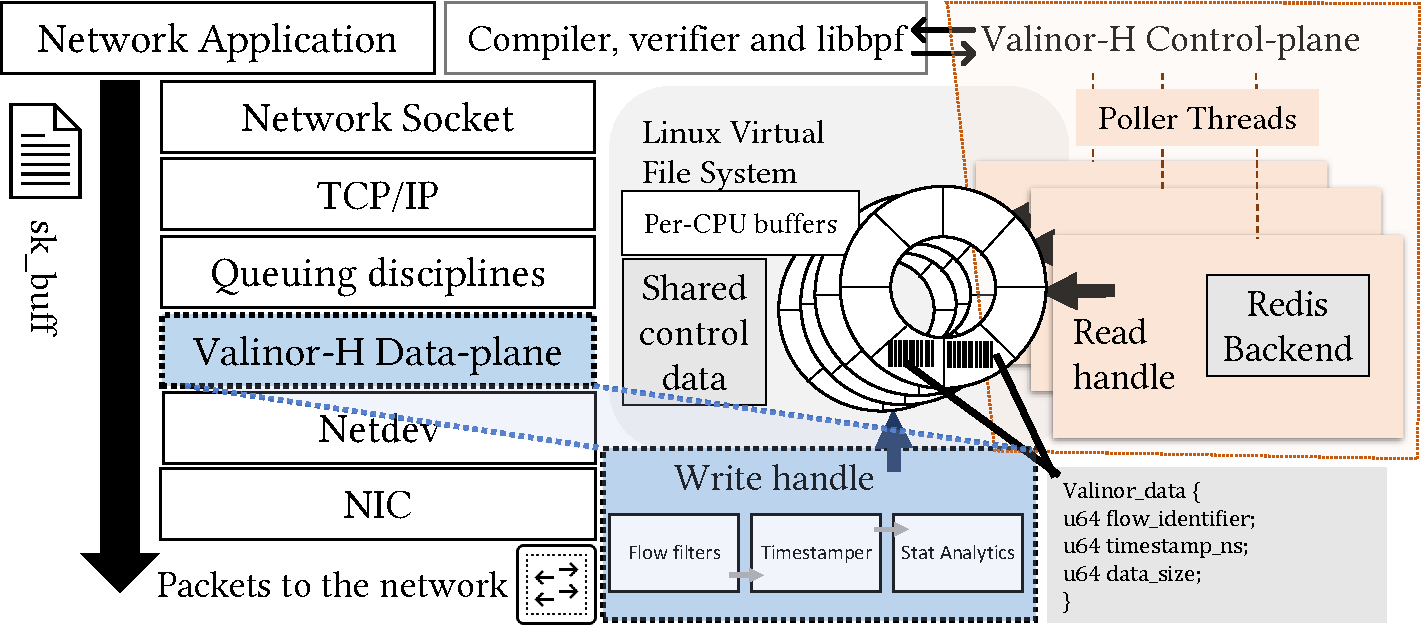
\includegraphics[width=0.85\linewidth]{figs/ebpf-crop.pdf}
      % \vspace{-4mm}
    \caption{\small{Valinor-H consists of an eBPF-based data plane and a control plane, communicating via lock-free ring buffers.}}
	\label{fig:bpf}
 % \vspace{-3mm}
\end{figure}

% \subsubsection{Framework design and implementation}
Figure \ref{fig:bpf} presents the design of our eBPF framework. Our framework consists of two separate programs. The data plane program follows a strict set of C-like instructions that are executed at the \textit{tc} qdisc, every time a \textit{sk\_buff} arrives. We design circular buffers capable of storing up to $2^{16}$ arbitrary data entries shared with the control plane. Then, the \textit{write handle} determines the correct location for adding new timestamp entries and updates the data structure. In the control plane, we initialize the data plane and the circular buffer and start polling the buffer for new data. The data entries carry the \textit{sk\_buff} lengths as well as the flow hash and protocol header information. The \textit{read handle}, retrieves the timestamp entries one by one and hands them to the Redis workers for persistent storage.

One challenge that arises when using a shared data structure is synchronization between the data plane and the control plane. This scenario generally needs locking mechanisms to prevent a race condition, however, the nature of the timestamping data, being strictly increasing, lifts this heavy burden. Therefore, in the control plane, Valinor-H only reads and increments its write handle if the timestamp value is larger than the previous value read.
Another synchronization issue arises when multiple CPUs attempt to store packet metadata in the shared memory. Luckily, eBPF offers per-CPU structures to prevent race conditions in the data plane. The Valinor-H control plane uses separate threads to read from per-CPU buffers simultaneously.

With the in-host measurement framework, network operators can verify the operation of higher-level network processing layers on the transmission path of the sender hosts. Valinor-H, at this stage, can capture the ingress traffic into the NIC which includes the traffic egress from qdiscs, the transport layer, and the applications. To capture the traffic behavior in the core of the network, and on a per-packet granularity, we introduce Valinor-N in the following section.


\subsection{Valinor-N: in-network burst measurement}
\label{sec:innetwork}


Software-based measurements in the host stack are bound to the coarse-grained \textit{sk\_buff} arrivals and are implemented before NIC functions (i.e., ring schedulers and segmentation offloads). Hence, the captured traffic behavior might not match that of the wire. To fill this gap, we introduce the in-network variant of Valinor based on programmable switch data planes.
Valinor-N consists of three pieces: 1) the switch component, 2) the collector data plane, and 3) the analysis component. Valinor-N is able to I) capture per-packet arrival timestamps with zero overhead outside the critical path, II) collect and store timestamp entries arriving at line rate, and III) perform various analyses on timestamp data to provide an in-depth image of the traffic burstiness at different scales. 
\\
\\
\textbf{Valinor Switch.} The switch data plane program uses \textit{mirroring} and \textit{timestamping} functionalities available in the PISA architecture. For every packet that matches user-defined flow filters, Valinor-N appends the arrival timestamp, queuing delay, and the size of the original packet along with its layer l-4 header information to a special IP packet with a pre-defined Valinor header. The packet is then sent to a collector server. The server machine, deployed outside the critical path of the communication between traffic endpoints, aggregates the timestamp information and performs the offline analysis.
\\
\\
\textbf{Timestamp collection.} The collector machine features a userspace packet processing framework based on DPDK that parses the arrived packets and stores the timestamp information along with flow metadata into an in-memory Redis \cite{redis} instance. Analysis of the timestamp data is then performed by querying the data store.
Receiving timestamp packets at line rate and storing them in persistent storage poses several scalability challenges to the design of the collector component. 
To ensure that software can drain NIC buffers at line rate, we designate multiple worker threads to read and process the incoming packets. After parsing timestamp headers, the worker threads extract the timestamp data and send them to additional worker threads that are responsible for communicating with Redis. The stored metadata is then retrieved by the analysis framework to perform  burst analysis using timestamps.

Valinor-N's Redis workers issue batched commands during idle periods to minimize interference with packet processing workers. We use Redis sorted sets to store timestamp entries sorted by arrival times since the packets that arrive at the collector may have a different order from the packets that arrive at the Valinor-N switch data plane. 
We use 1G \textit{hugepages} and large memory pools to ensure that timestamp packets are not dropped at higher rates (Up to 40~Gbps in our testbed).
\\
\\
\textbf{Offline timestamp processing.} The last piece of Valinor's design is the offline timestamp analysis framework that queries the Redis data structures and performs analysis on timestamp data. Our framework is able to report various statistics on traffic burstiness by measuring the packet inter-arrivals. For example, in the next section, we report our findings on the scaling behavior, caused by various packet processing components in the sender machine. We report actual burst sizes in bytes, inter-arrival distributions, queueing delays, and various burstiness time series analyses. We implement the offline processing framework in Python.


% \begin{figure}[t]
% \centering
% \begin{subfigure}[t]{0.52\linewidth}
%     \centering
%     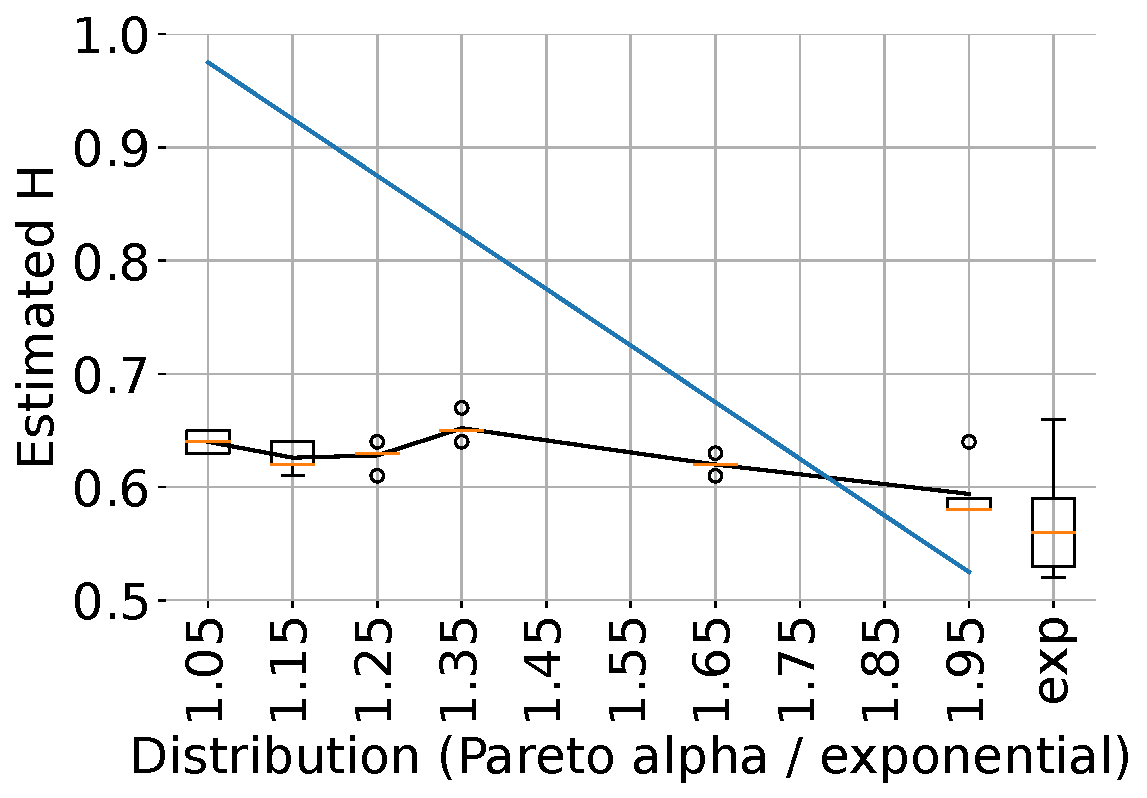
\includegraphics[width=1\linewidth]{figs/filehurst_ebpf_testbed.pdf}
%     \caption{\small{\textbf{Synthetic-Hurst exponents}}}
% 	\label{fig:fhurst-ebpf}
% \end{subfigure}
% \begin{subfigure}[t]{0.46\linewidth}
%     \centering
%     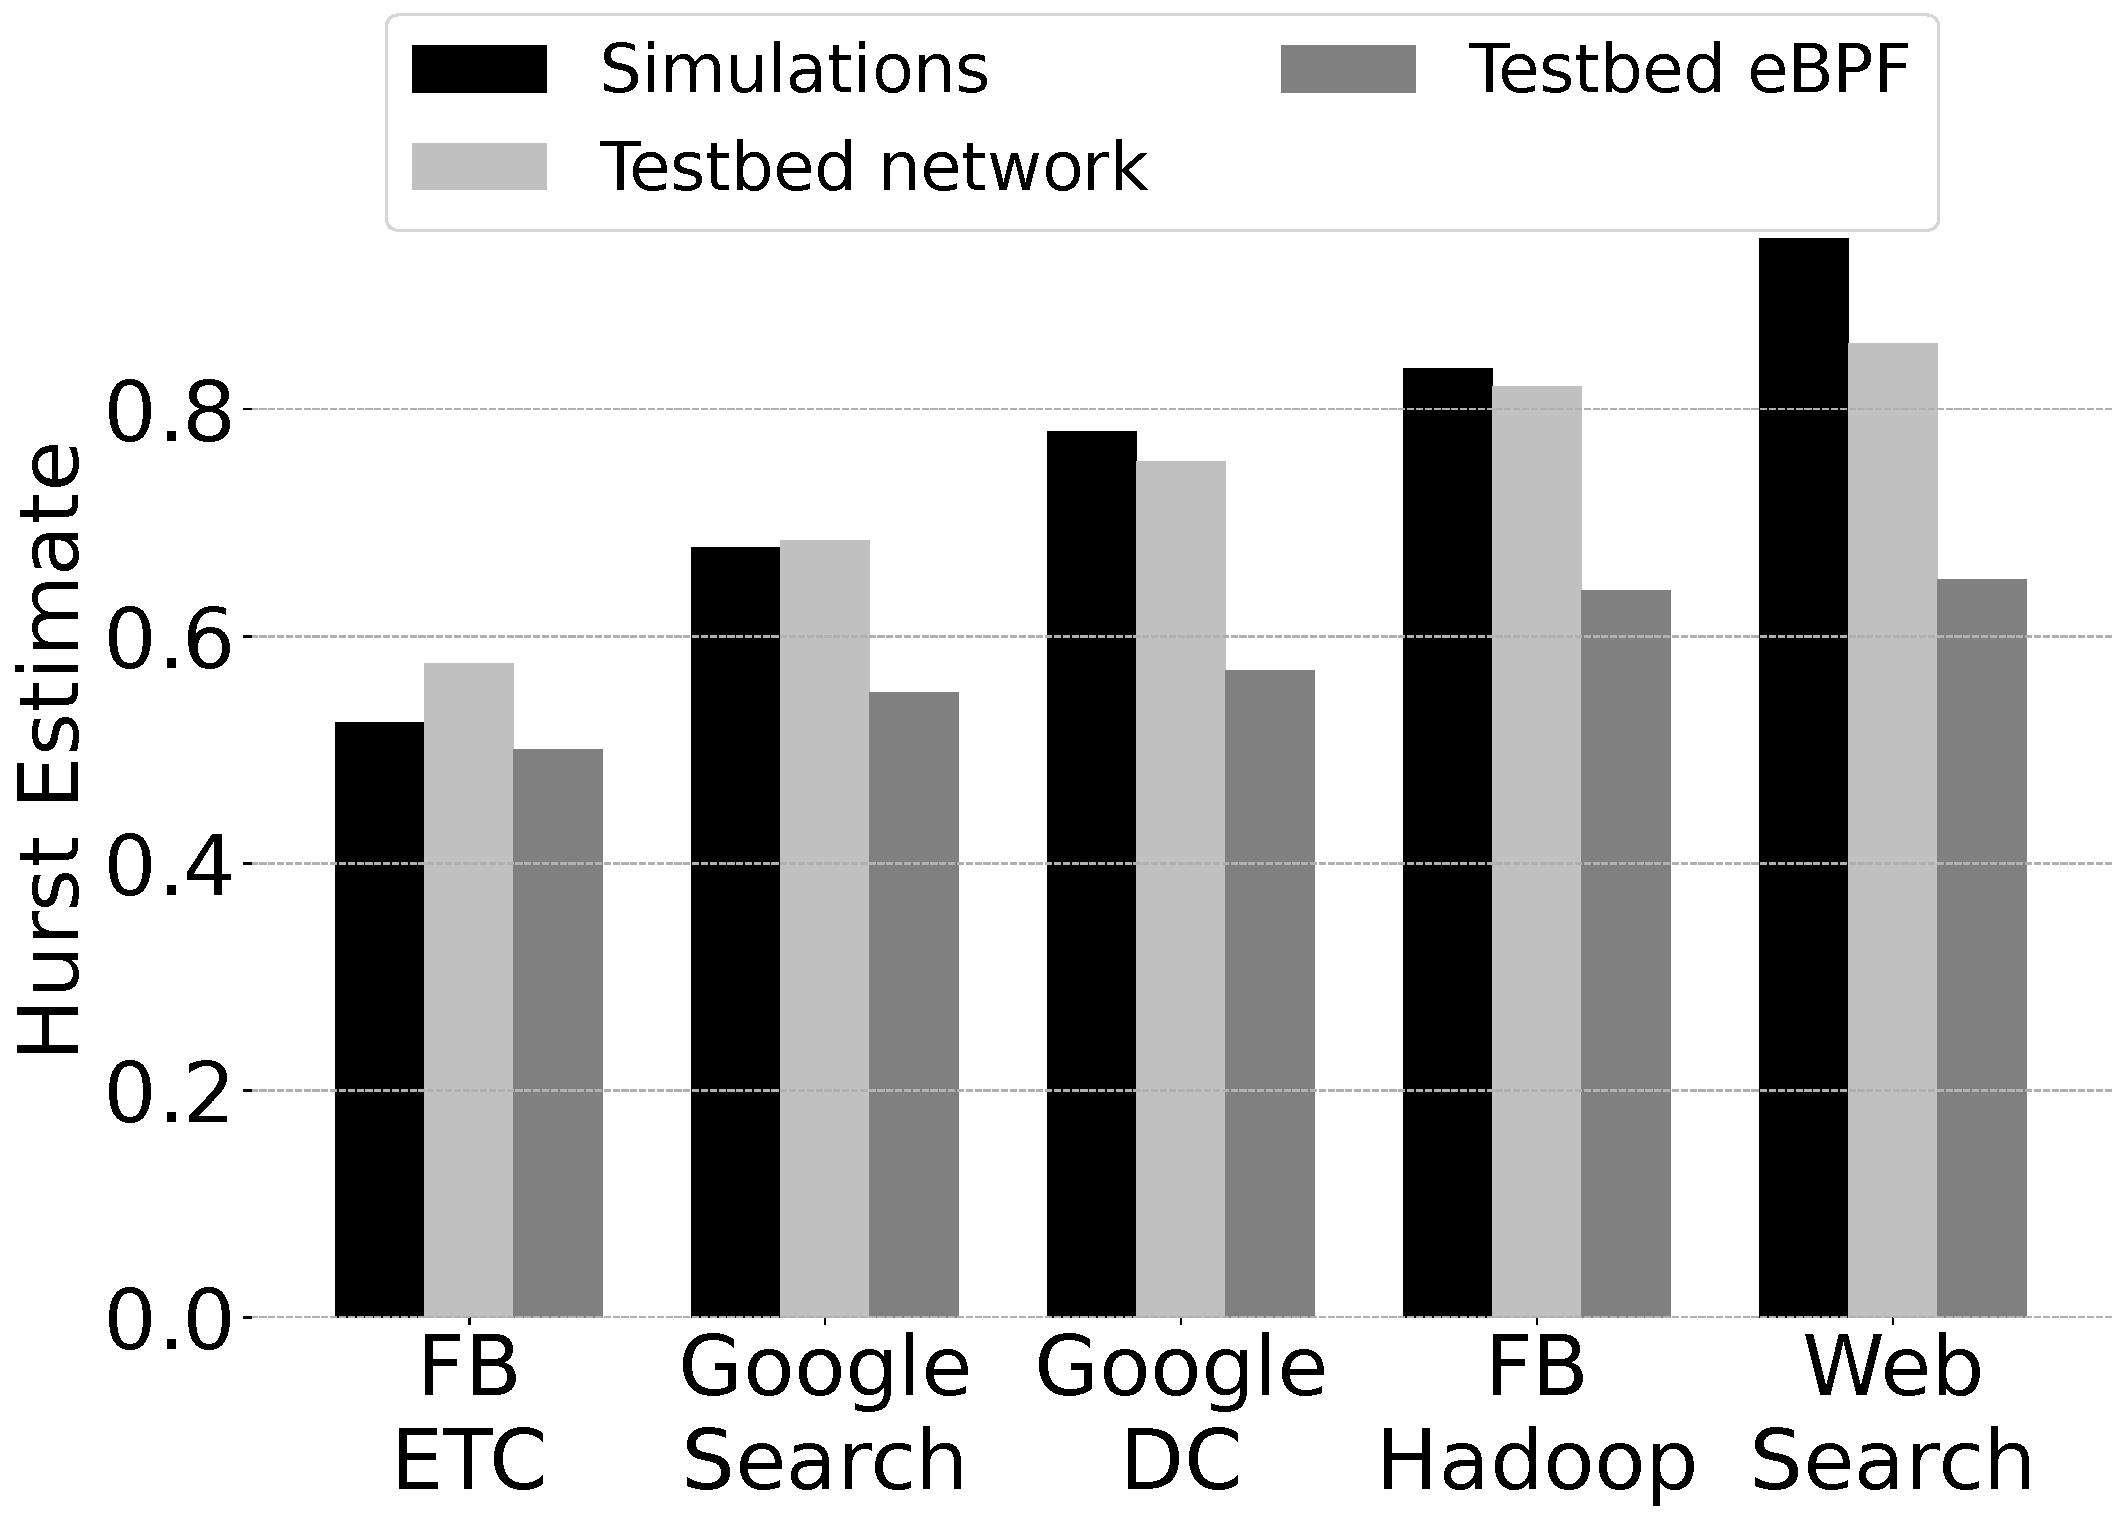
\includegraphics[width=1\linewidth]{figs/w_ebpf_hurst_bar.pdf}
%     \caption{\small{\textbf{Trace-Hurst exponents}}}
% 	\label{fig:whurst-ebpf}
% \end{subfigure}
% \begin{subfigure}[t]{0.49\linewidth}
%     \centering
%     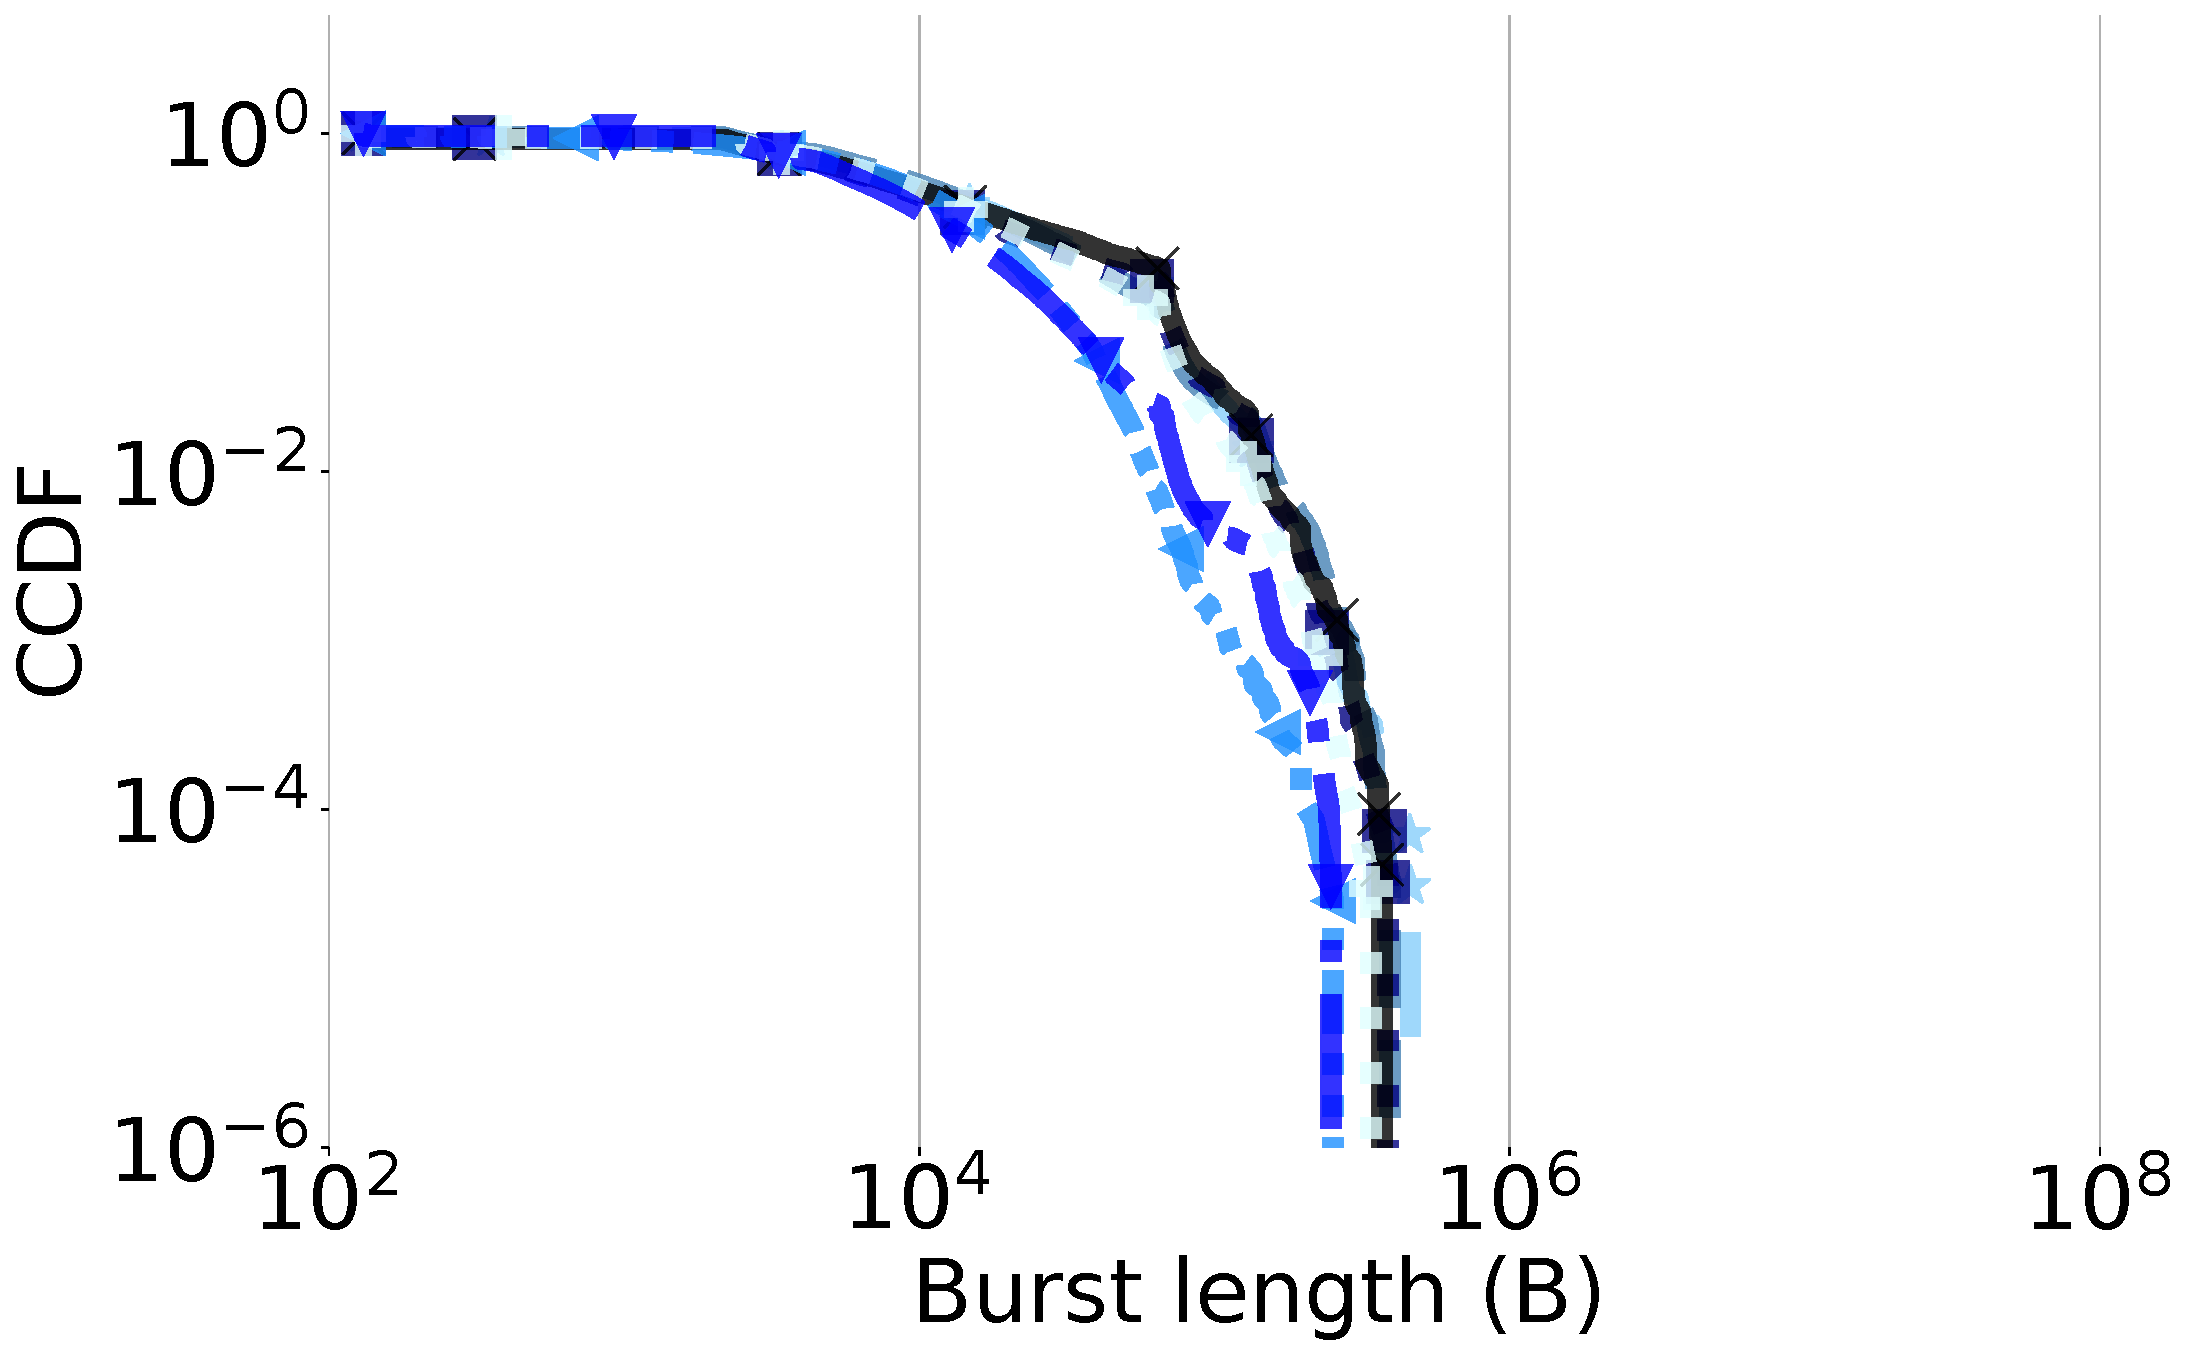
\includegraphics[width=1\linewidth]{figs/fileccdf_ebpf_testbed.pdf}
%     \caption{\small{\textbf{Synthetic-burst length CCDF}}}
% 	\label{fig:fccdf-ebpf}
% \end{subfigure}
% \begin{subfigure}[t]{0.49\linewidth}
%     \centering
%     	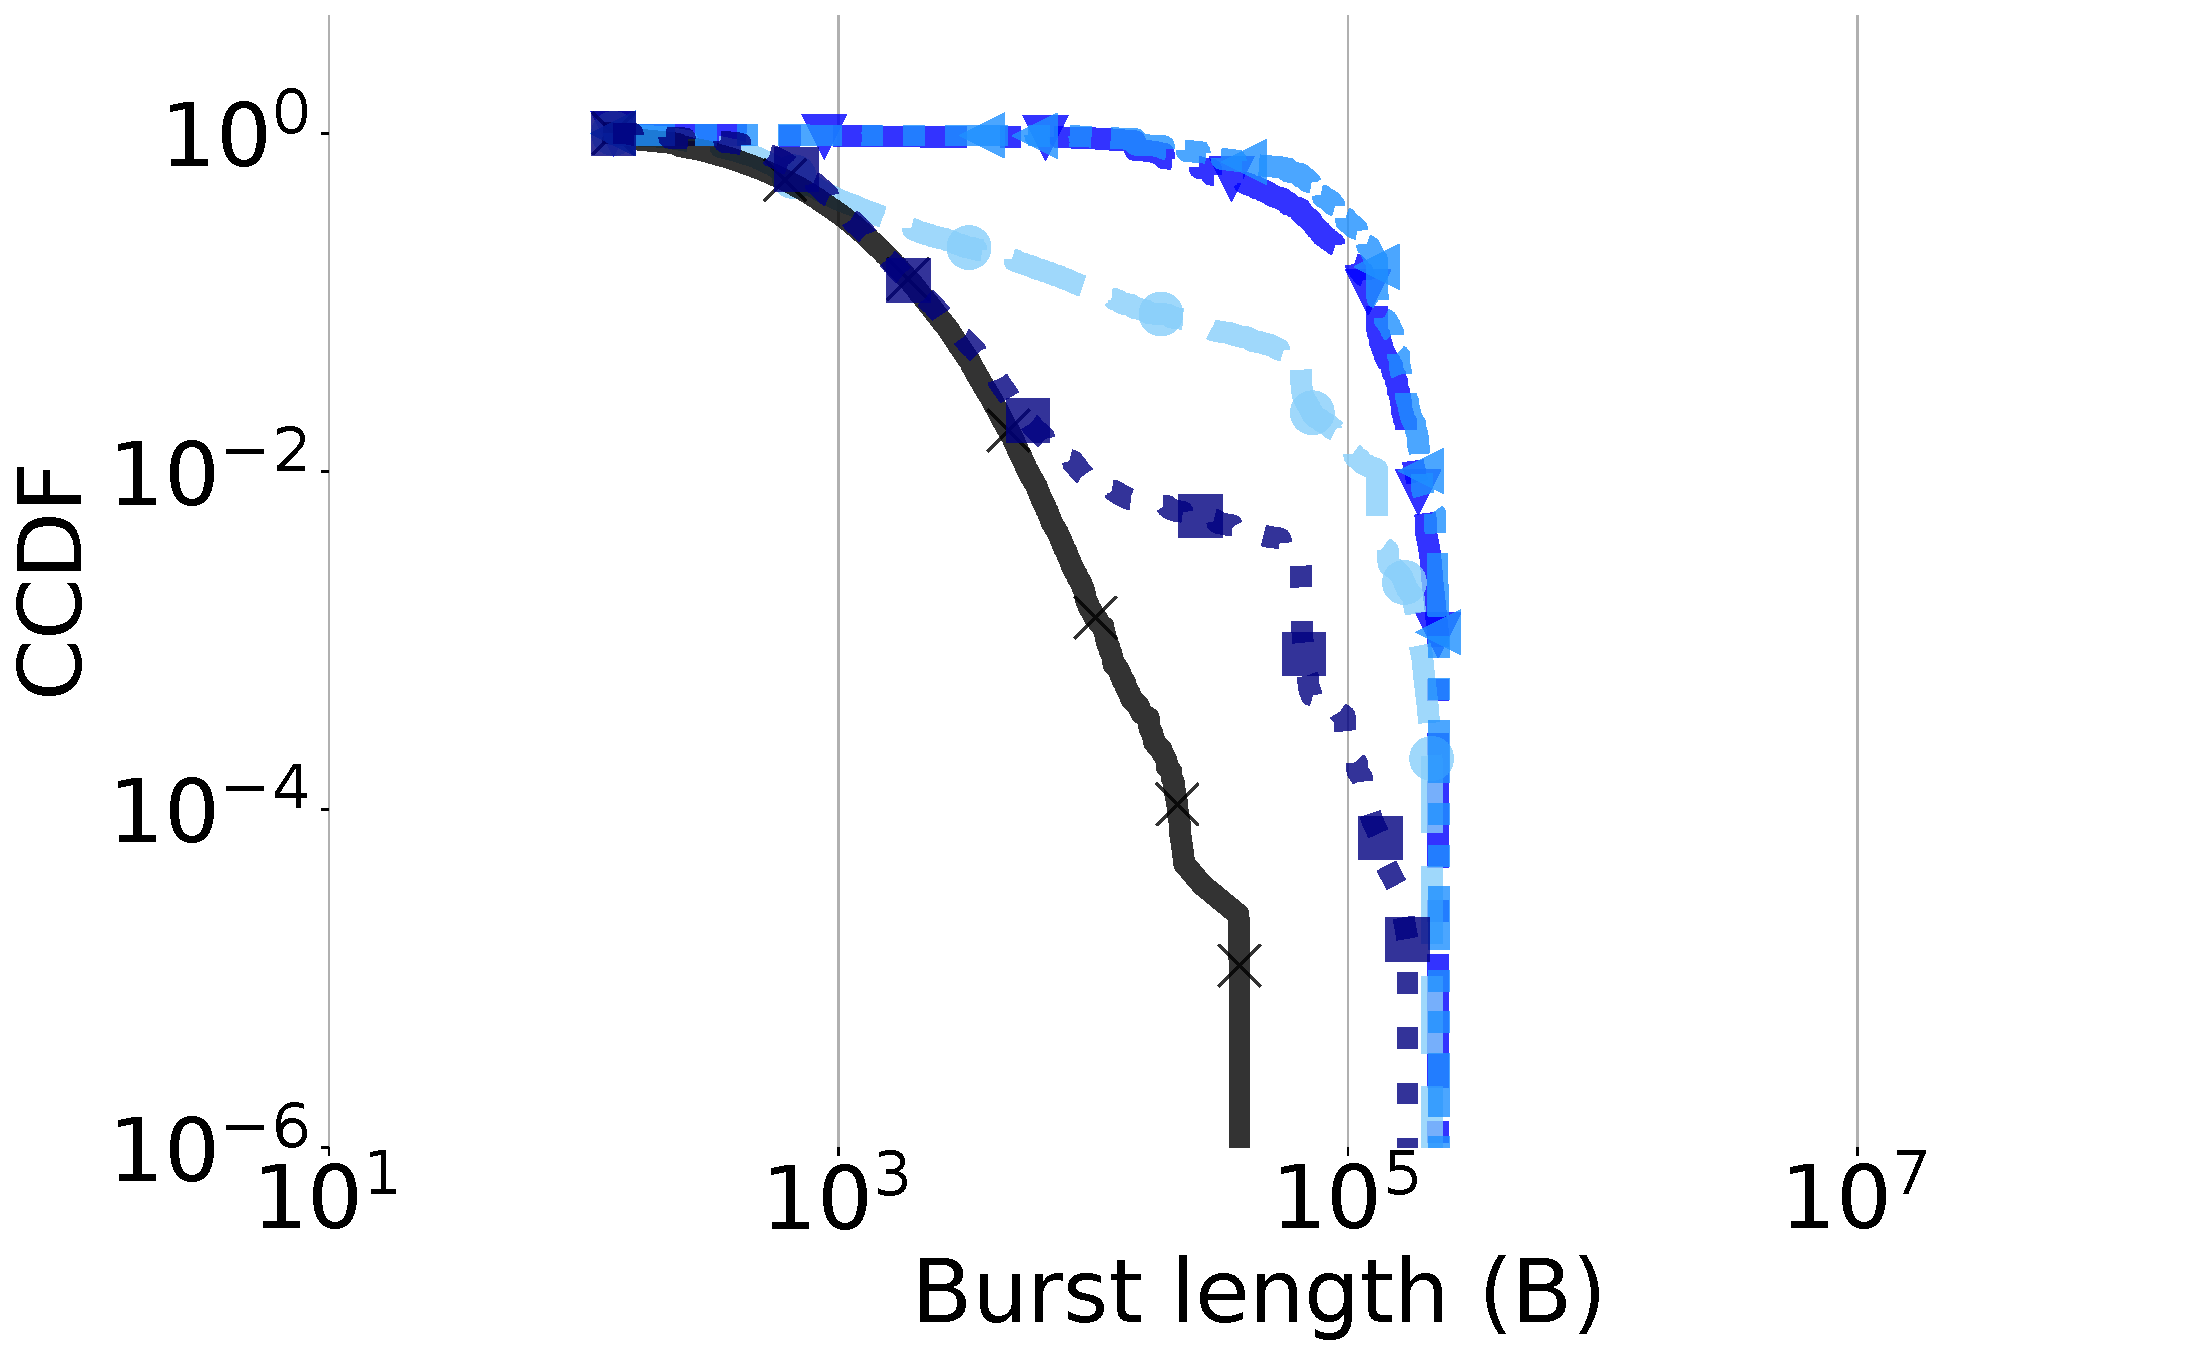
\includegraphics[width=1\linewidth]{figs/wccdf_ebpf_testbed.pdf}
%     \caption{\small{\textbf{Trace-burst length CCDF}}}
% 	\label{fig:fwccdf-ebpf}
% \end{subfigure}
%     \caption{\textbf{\small{\erfan{Repeating synthetic and trace experiments with eBPF framework. Because of the coarser-grained measurements and being placed behind the NIC functions, Valinor-H presents a smoother trend for burstiness compared to Valinor-N. However, Valinor-H is still able to show a relatively accurate picture of the expected traffic burstiness within the host machine.}}}}
% 	\label{fig:ebpf}
% \end{figure}

We deploy Valinor to analyze the burstiness of various workloads and configurations.
%We perform simulations and testbed experiments using the above implementation of Valinor. 
Our results show:
\begin{compactitem}
    % \item \st{Flow-based packet scheduling can have a considerable  impact on blunting microbursts for egress traffic.}\soudeh{Only true for SQ, no offloading (unrealistic).}
    \item Host networking, largely overlooked in prior self-similarity studies, plays a major role in forming and suppressing bursts.
    %Unlike previous conceptions about directly attributing the sources of burstiness to the workload and applications, host networking elements play a key role in reshaping the original workload. 
    
    \item Lower layers of the network processing stack (such as segmentation offloading and NIC scheduling) compromise the effectiveness of software-based traffic shaping and active queue management solutions.
    
    \item Software pacing has major limitations. For workloads with a mixture of short and large flows, lower layers of the network processing stack mask the impact of software-based traffic pacing. For workloads with very short flows, software pacing can blunt bursts but leads to a major increase in RTT and significant throughput reduction. 
    % \st{Software pacing presents inconsistent burstiness behavior towards workloads with different size distributions. }
    
    \item NIC driver buffer sizing and process scheduling can reshape bursts.
\end{compactitem}


\section{Findings}
\label{sec:valinor-findings}
\begin{figure}[t]
    \centering
    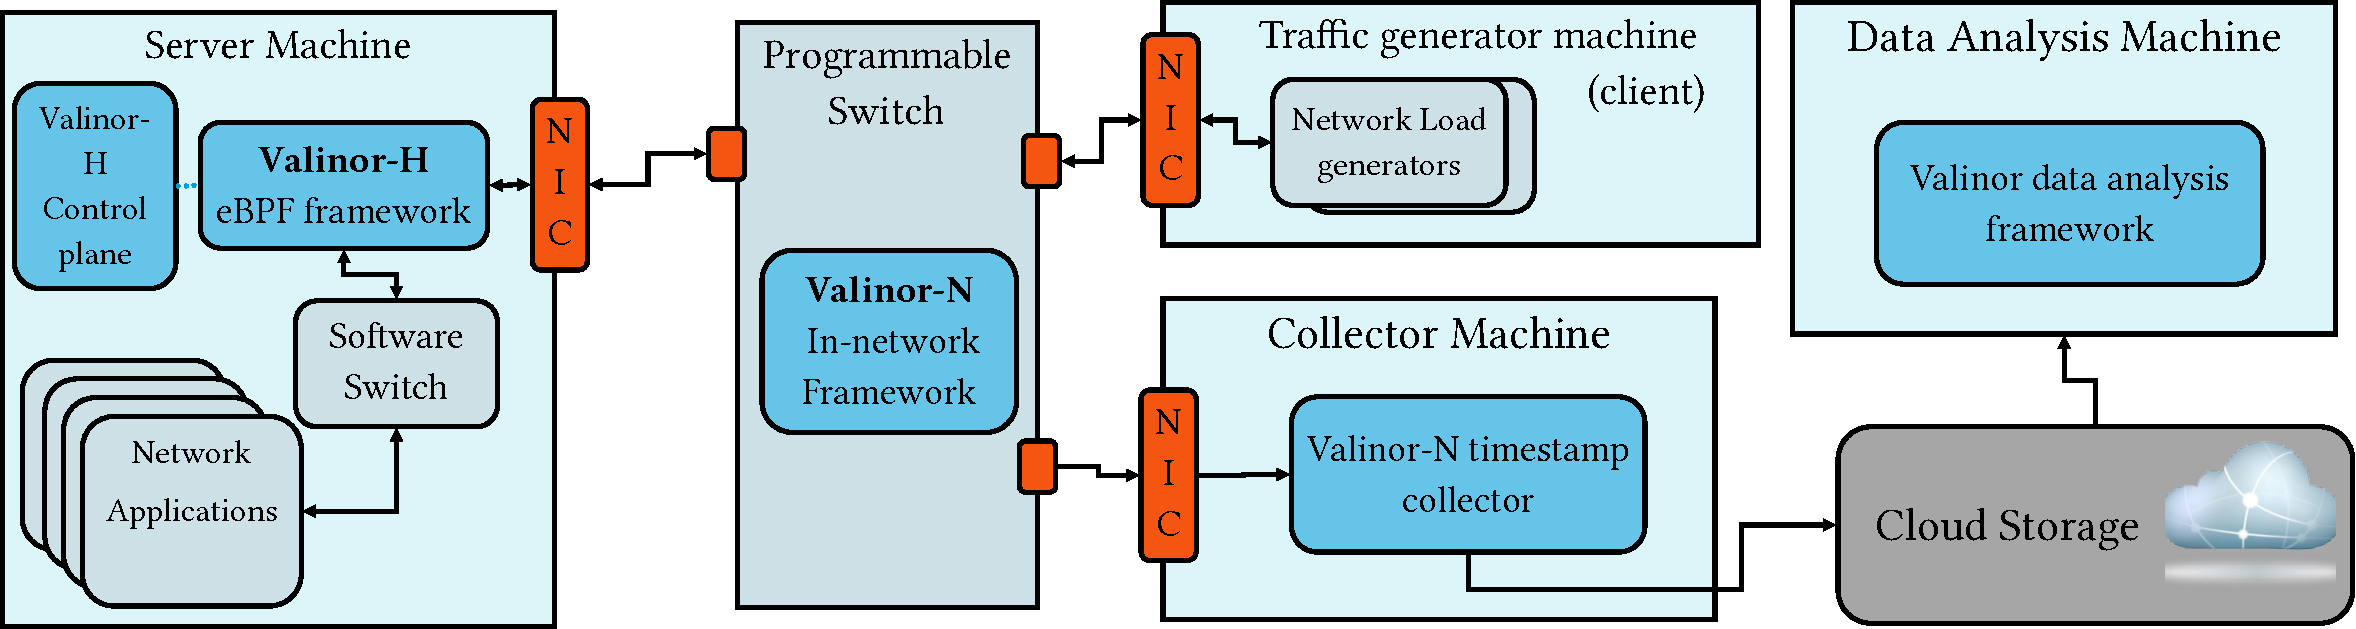
\includegraphics[width=0.9\linewidth]{figs/setup-crop.pdf}
     \vspace{-3mm}
    \caption{\small{Valinor framework deployment overview.}}
	\label{fig:setup}
 \vspace{-2mm}
\end{figure}
% \begin{subfigure}[t]{0.9\linewidth}
%     \centering
%     	\includegraphics[width=0.85\linewidth]{figs/21-2_summary_21_0.png}
%     \caption{\small{Burst behavior of Linux queueing disciplines in the presense of offloading.}}
% 	\label{fig:qdisc_tso}
% 	\end{subfigure}


% \begin{figure}
% \centering
%     	\includegraphics[width=1\linewidth]{figs/qdisc2.pdf}
%     \caption{\small{Impact of per-flow deficits in fq qdisc on traffic burstiness. \erfan{FINALIZED}}}
% 	\label{fig:qdisc_quantum}
% \end{figure}


\paragraph{Experiment setup.}
% We deploy Docker containers hosting applications that resemble widely deployed workloads in data centers. We deploy Memcached for key-value, an in-house restful HTTP server for Web, and Iperf3 containers for throughput heavy workloads. All containers are connected via an OVS \cite{ovs} virtual bridge to the external port. We generate Cache and web workloads using our modified version of Mutilate, based on Facebook's CDF distributions \cite{social}. Our testbed consists of three servers with 1x Intel Xeon  E5-2620 v4 processors, 64 GB of memory and Intel XL710 40G RNICs. We connect the servers via a Wedge Tofino switch augmented with Valinor's timestamping framework. The collector machine features Valinor userspace dataplane based on DPDK v20. We disable idle-states on all servers and set the frequency governor to \textit{performance} to minimize the interference of power-saving features on networking performance.
% Finally, we store the redis data dumps in Azure SMB data shares and use a Cloudlab \cite{cloudlab} server to process the timestamp data.
Figure \ref{fig:setup} demonstrates how Valinor framework components come together in a basic deployment.
For evaluating Valinor, we use a wide range of workload distributions. We deploy Iperf instances alongside Homa's open-source load generator \cite{homa} inside Linux containers and configure the workload generators to simulate different trace-driven workload patterns including Facebook's ETC, Google search, aggregated Google data center, DCTCP's web search, and Facebook's intra-cluster and intra-rack Hadoop traces \cite{social,homa,fb-workload,dctcp}. Unless stated otherwise, all application containers are connected via an \textit{OVS} \cite{ovs} virtual bridge to the external interface.
% For more realistic traces, we preload Memcached \cite{memcached} according to publicly available data center flow size distributions and use a modified version of Mutilate to generate requests using public inter-arrival distributions \cite{social}.
Our testbed consists of servers featuring Intel Xeon  E5-2620 v4 processors, 64 GB of memory, and Intel XL710 40G NICs. We connect the servers via a Wedge-100 Tofino switch running Valinor-N timestamping framework. We deploy Valinor-H on Linux kernel 5.17 with the latest version of \textit{libbpf} and \textit{iproute2} installed. The collector machine features Valinor's userspace data plane based on \textit{DPDK} v20. We disable idle states on all servers and set the frequency governor to \textit{performance} to minimize the interference of power-saving features on networking performance.
The default settings for the evaluated components are summarized in Table \ref{tab:ranges}.

Finally, to calculate microburst lengths, since we use 40Gbps links, we set the burst inter-arrival threshold to 500ns for the presented results (see \S\ref{sec:valinor-background}). Valinor also computes microburst lengths for other threshold settings (ranging from 5ns to 10$\mu$s). 
While the threshold setting impacts the size and quantity of observed bursts, we did not notice any difference in relative burstiness when comparing multiple cases.
We have released Valinor's sources and artifacts as open-source software.\footnote{\url{https://hopnets.github.io/valinor}}
% Finally, we store the Redis data dumps in Azure SMB data shares and use a Cloudlab \cite{cloudlab} server to process the timestamp data

% \subsection{Comparing the burstiness of three different workloads.}
% We run \textit{Iperf3}, \textit{Memcached}, and \textit{HTTP} workloads and generate load using \textit{Iperf3 client}, and \textit{Mutilate}, respectively. Figure \ref{fig:three_workloads} presents the difference in the burstiness of three workloads when we configure the load to use up all the CPU cores of the server machine. \erfan{Experiment in progress}

\begin{table}[t]
\centering

\begin{tabular}{l|l|l}
\textbf{Setting}           & \textbf{Default Value} & \textbf{Parameter Range}                                \\ \hline \hline
Transport         & TCP cubic     & cubic, reno, BBR, DCTCP, Homa        \\ \hline
Qdisc             & fq            & fq, fq\_codel, pfifo\_fast, HHF, SFQ \\ \hline
Byte Queue Limit  & Dynamic       & 100B-10MB                      \\ \hline
MTU               & 1500          & 1500, 9000                           \\ \hline
Process scheduler & CFS           & CFS, FIFO, Microquanta               \\ 
\end{tabular}
\caption{\small{Default system configuration and tested parameter ranges for Valinor.}}
	\label{tab:ranges}
\end{table}

\begin{figure}[t]
\centering
\begin{subfigure}[t]{0.49\linewidth}
    \centering
    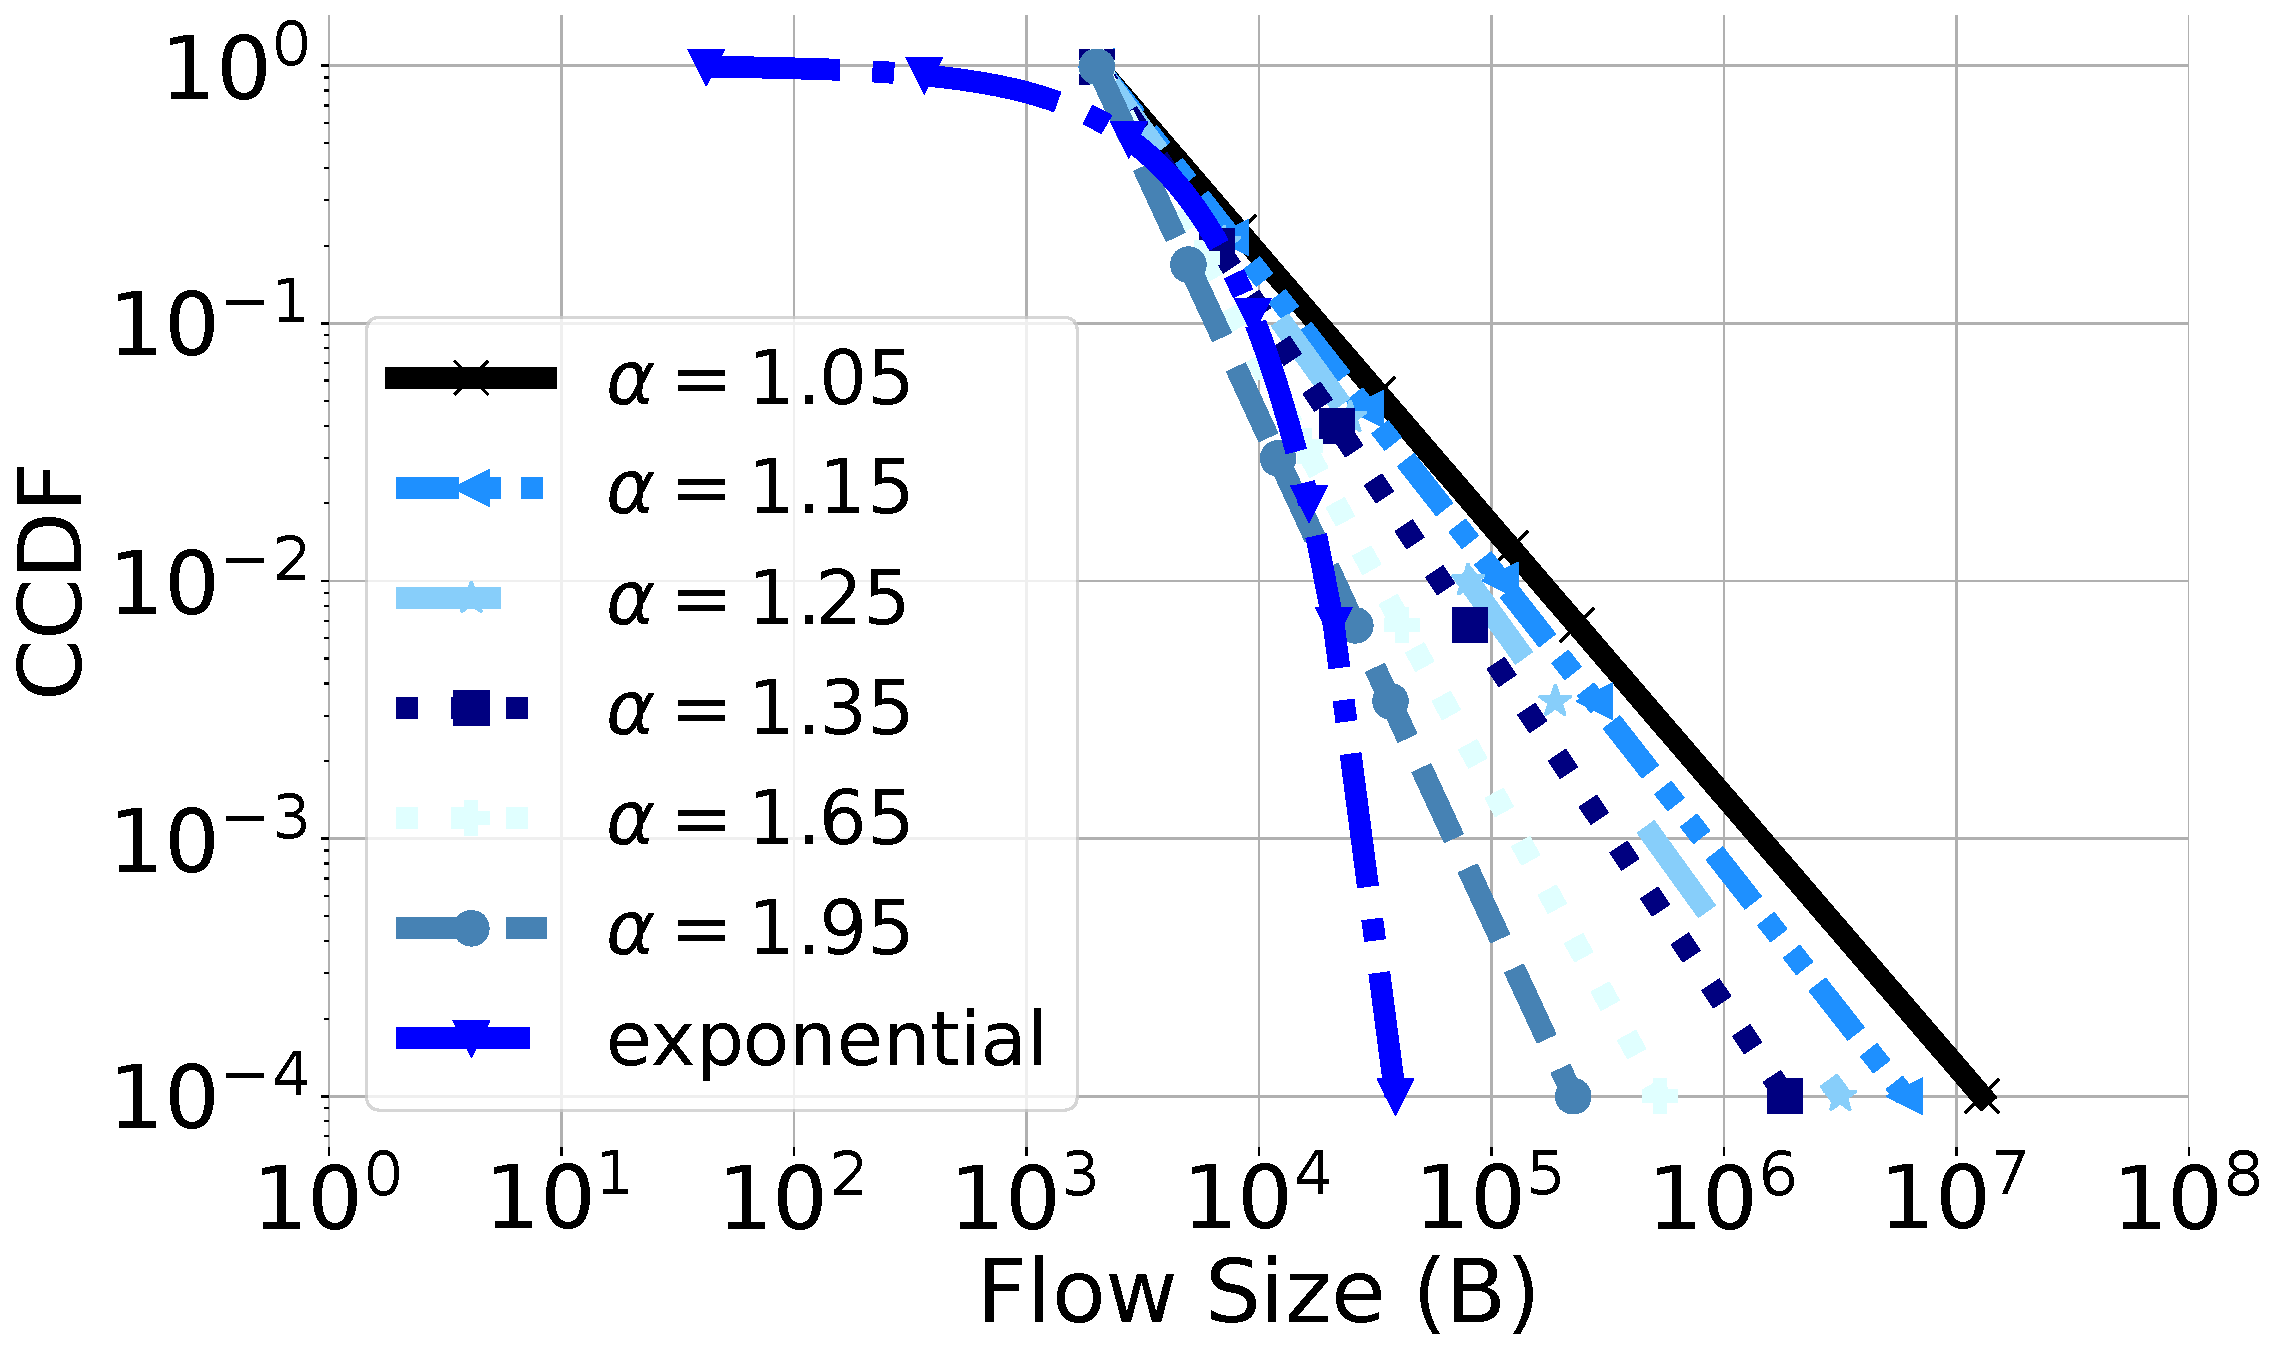
\includegraphics[width=1\linewidth]{figs/syntheticcdf_fsize_large.pdf}
    \caption{Synthetic workload}
	\label{fig:filecdf-dist}
\end{subfigure}
\begin{subfigure}[t]{0.49\linewidth}
    \centering
    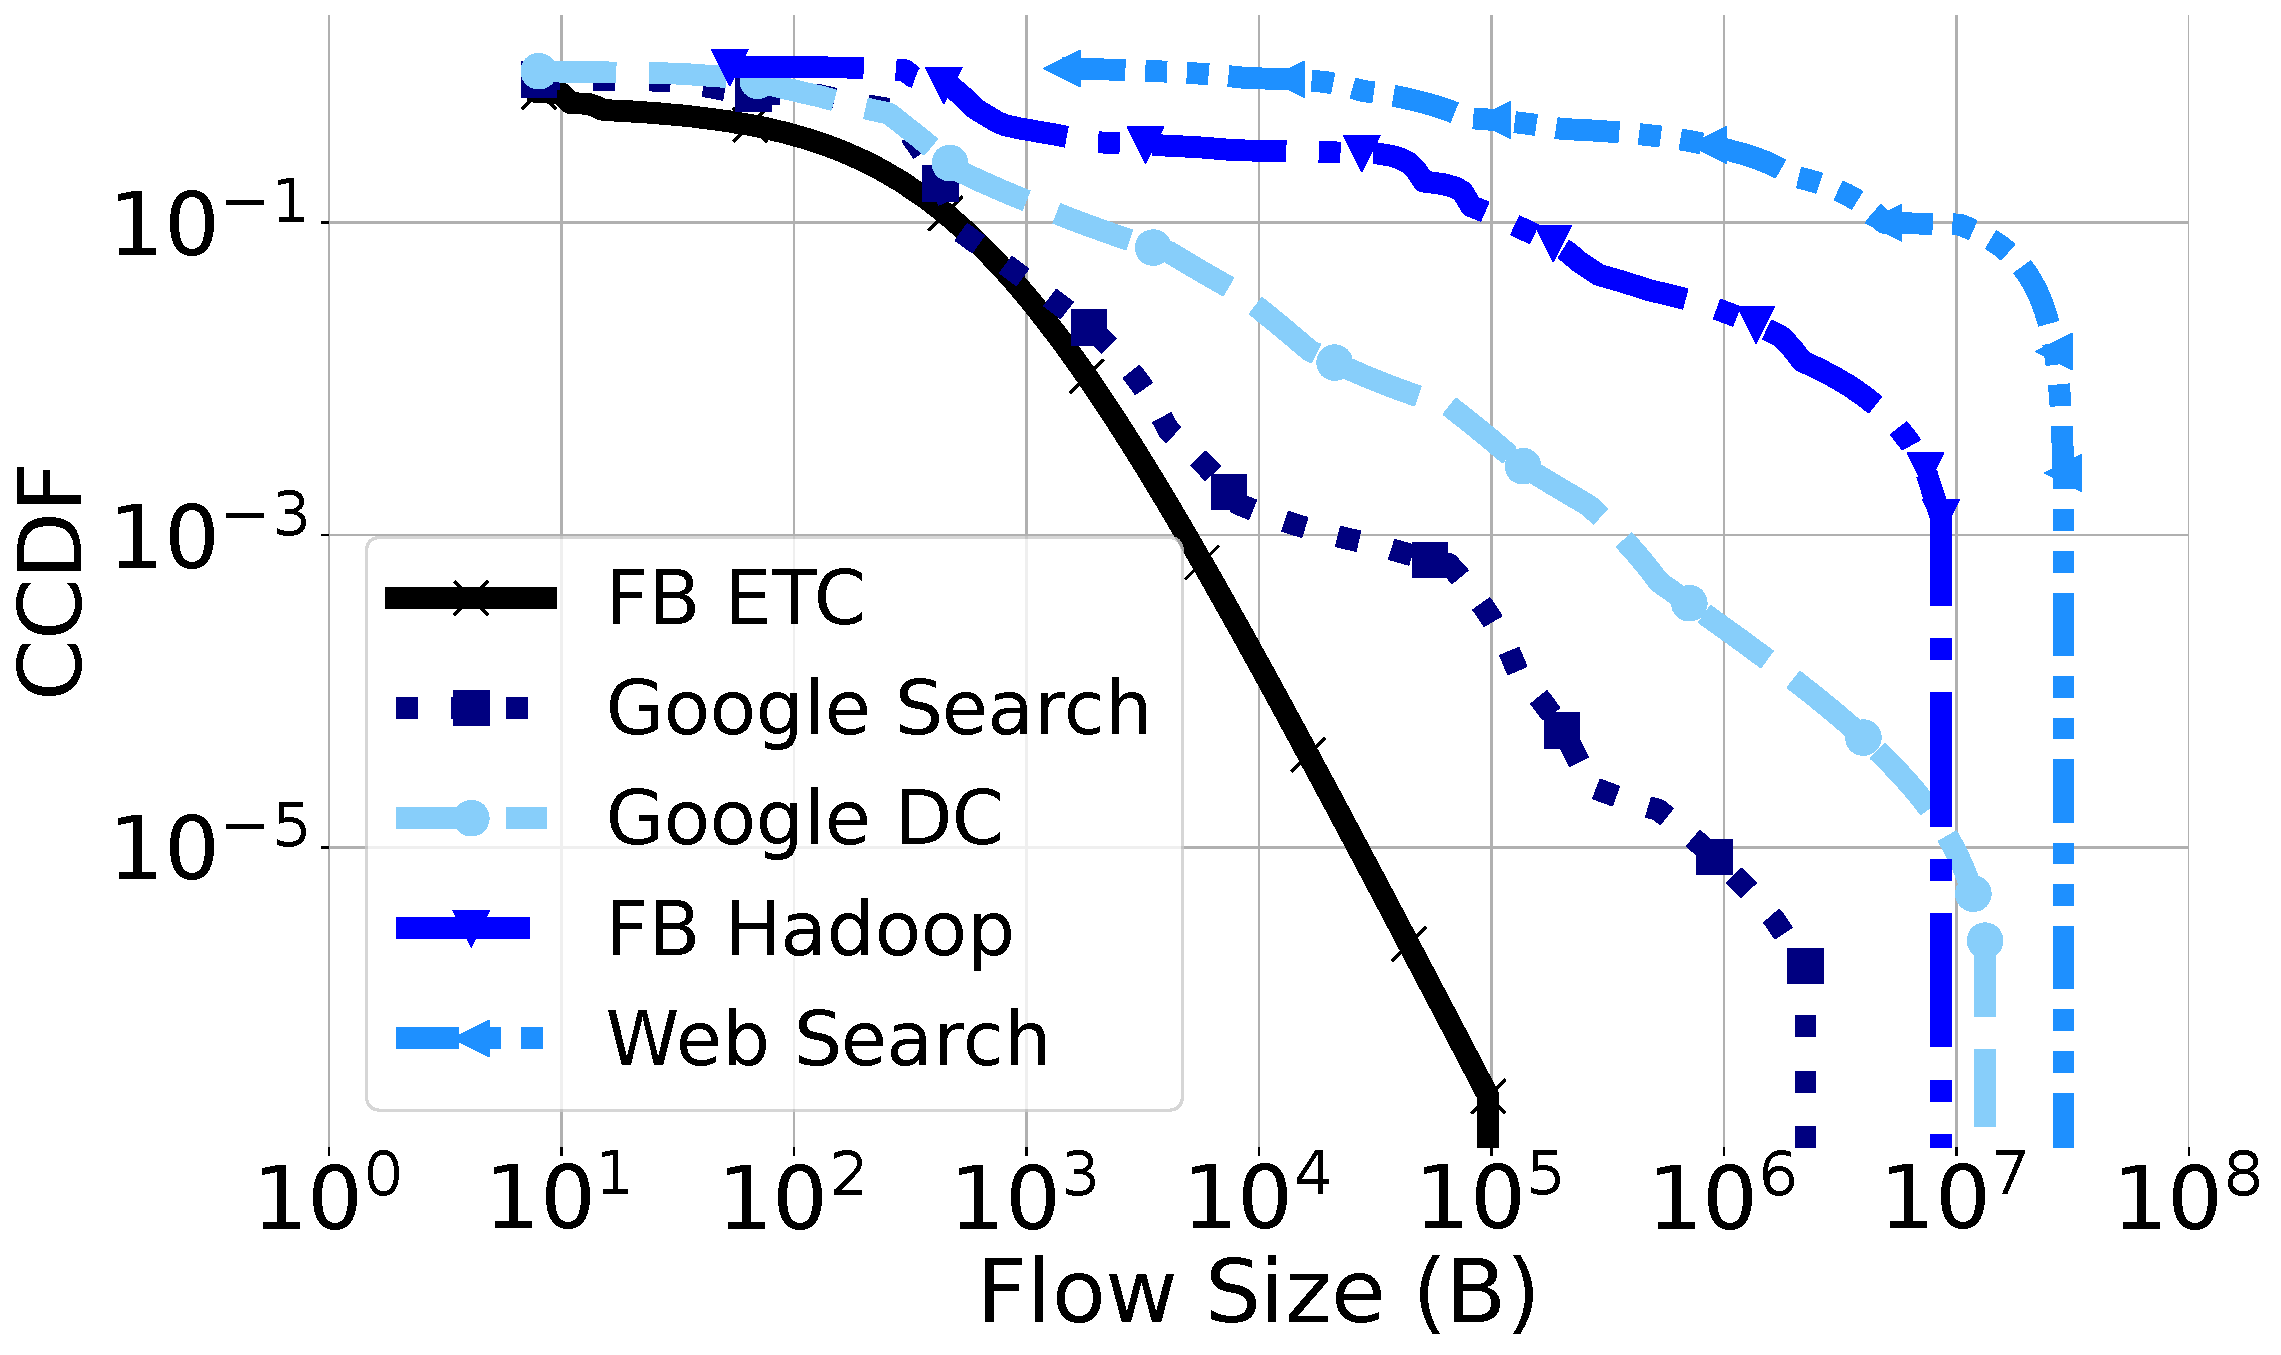
\includegraphics[width=1\linewidth]{figs/wccdf_fsize.pdf}
    \caption{Trace-driven workload}
	\label{fig:trace-ccdf}
\end{subfigure}
 % \vspace{-2mm}
    \caption{\small{Two sets of workloads used throughout the experiments. The figures show the complementary cumulative distribution functions (CCDFs) of flow sizes.}}
	\label{fig:distributions}
 % \vspace{-3mm}
\end{figure}


\begin{figure}[t]
\centering
\begin{subfigure}[t]{0.32\linewidth}
    \centering
    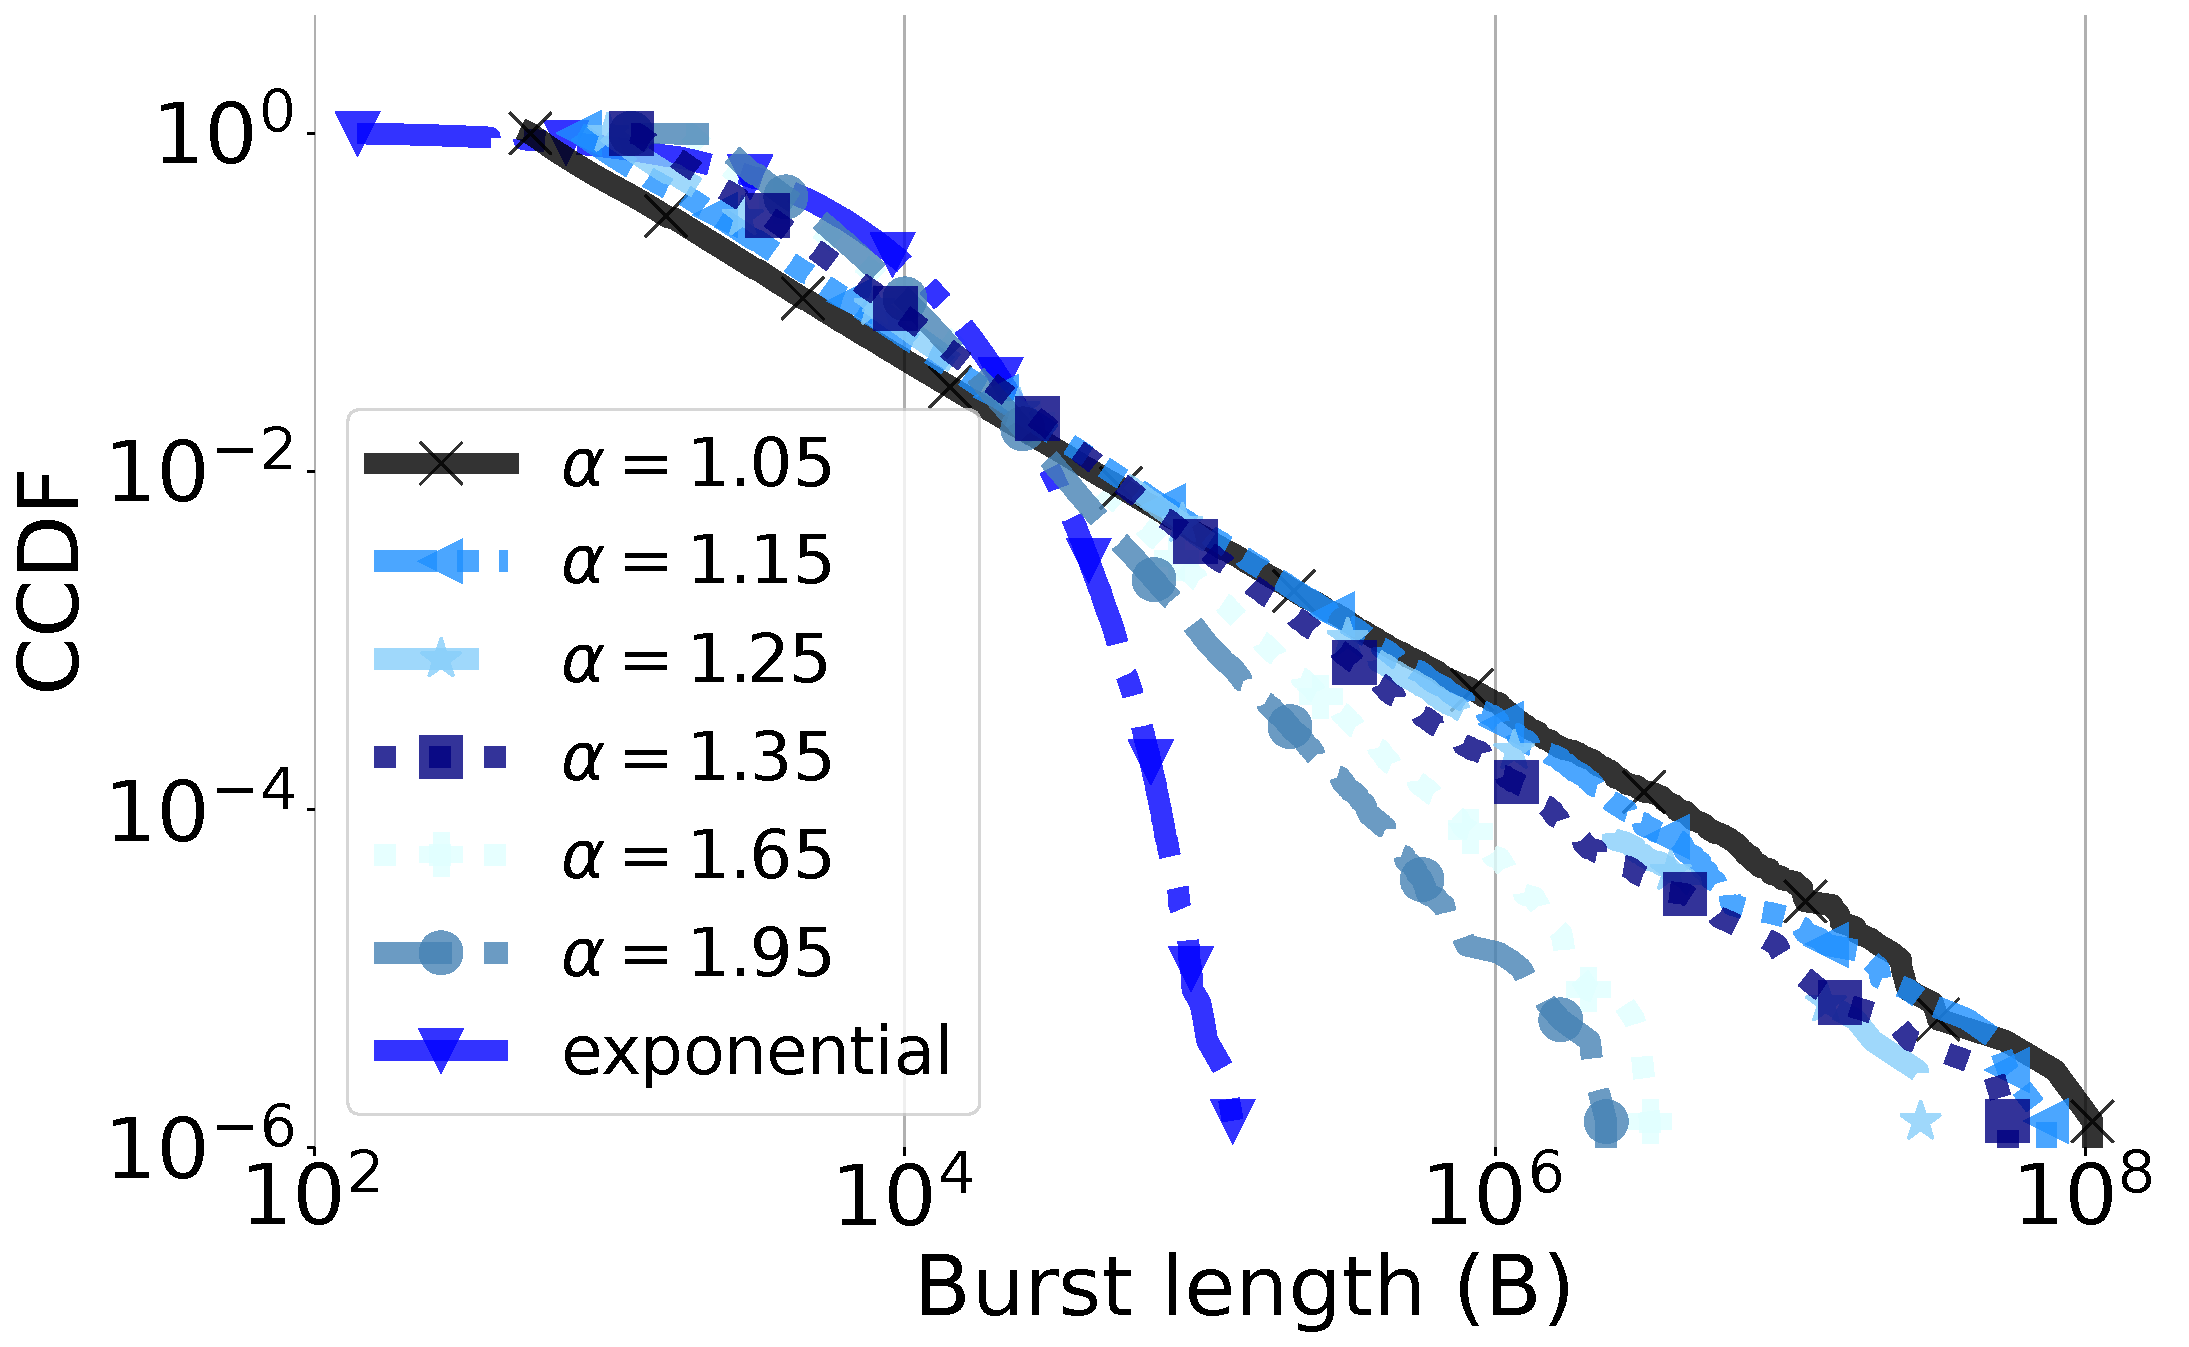
\includegraphics[width=1\linewidth]{figs/fileccdf_sim.pdf}
    \caption{Simulation microbursts}
	\label{fig:filecdf-sim}
\end{subfigure}
\begin{subfigure}[t]{0.32\linewidth}
    \centering
    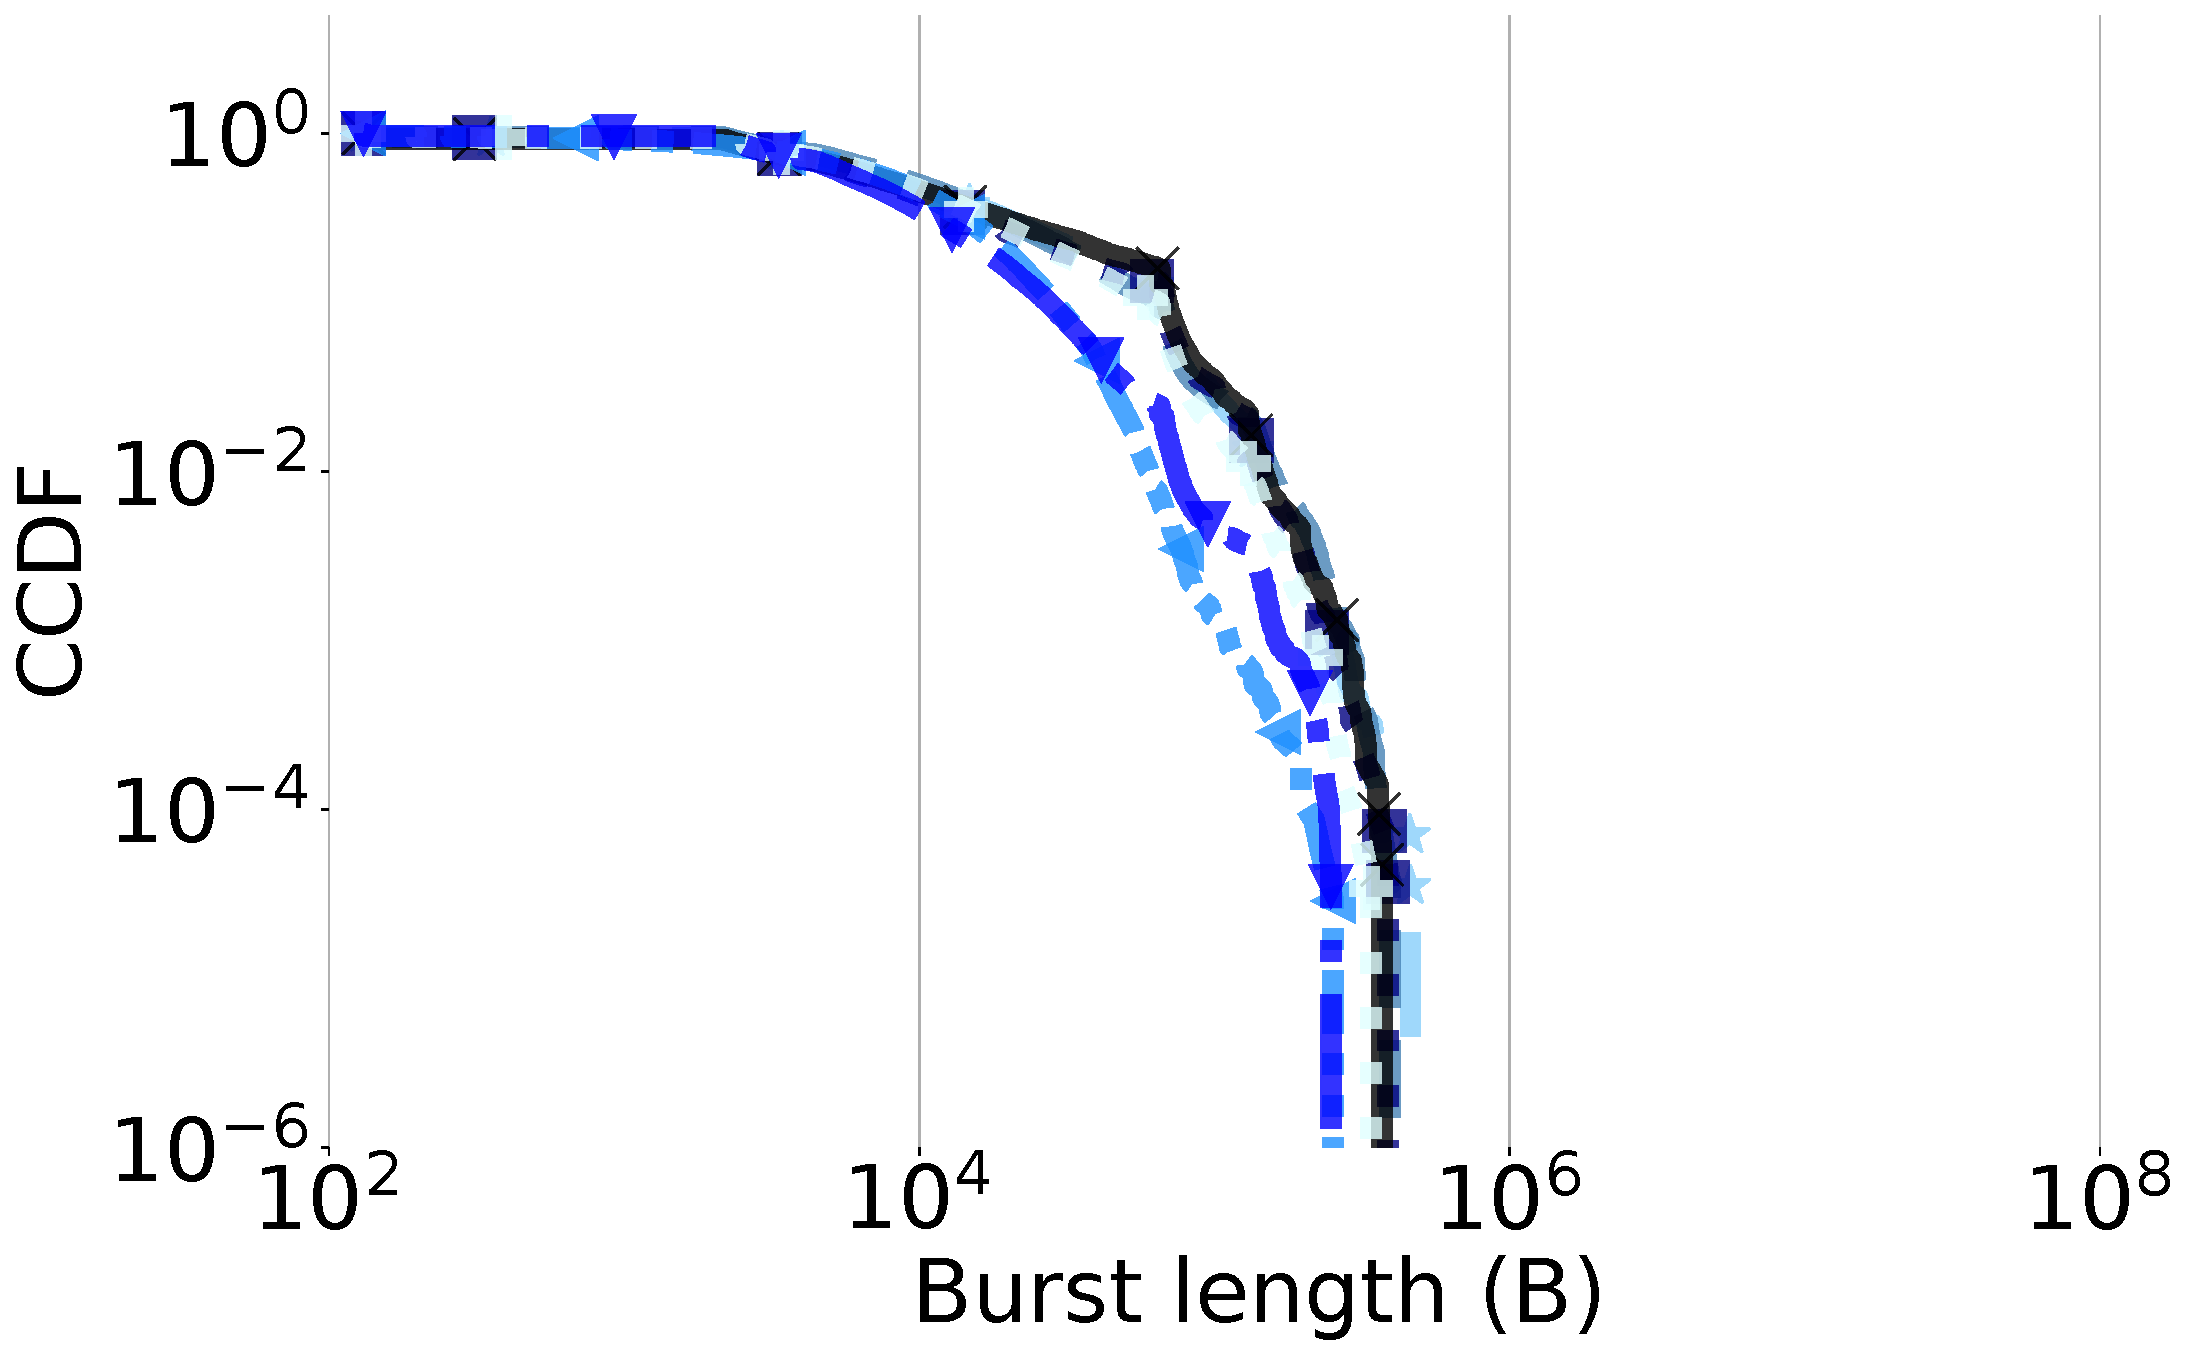
\includegraphics[width=1\linewidth]{figs/fileccdf_ebpf_testbed.pdf}
    \caption{In-host microbursts}
	\label{fig:fccdf-ebpf}
\end{subfigure}
\begin{subfigure}[t]{0.32\linewidth}
    \centering
    	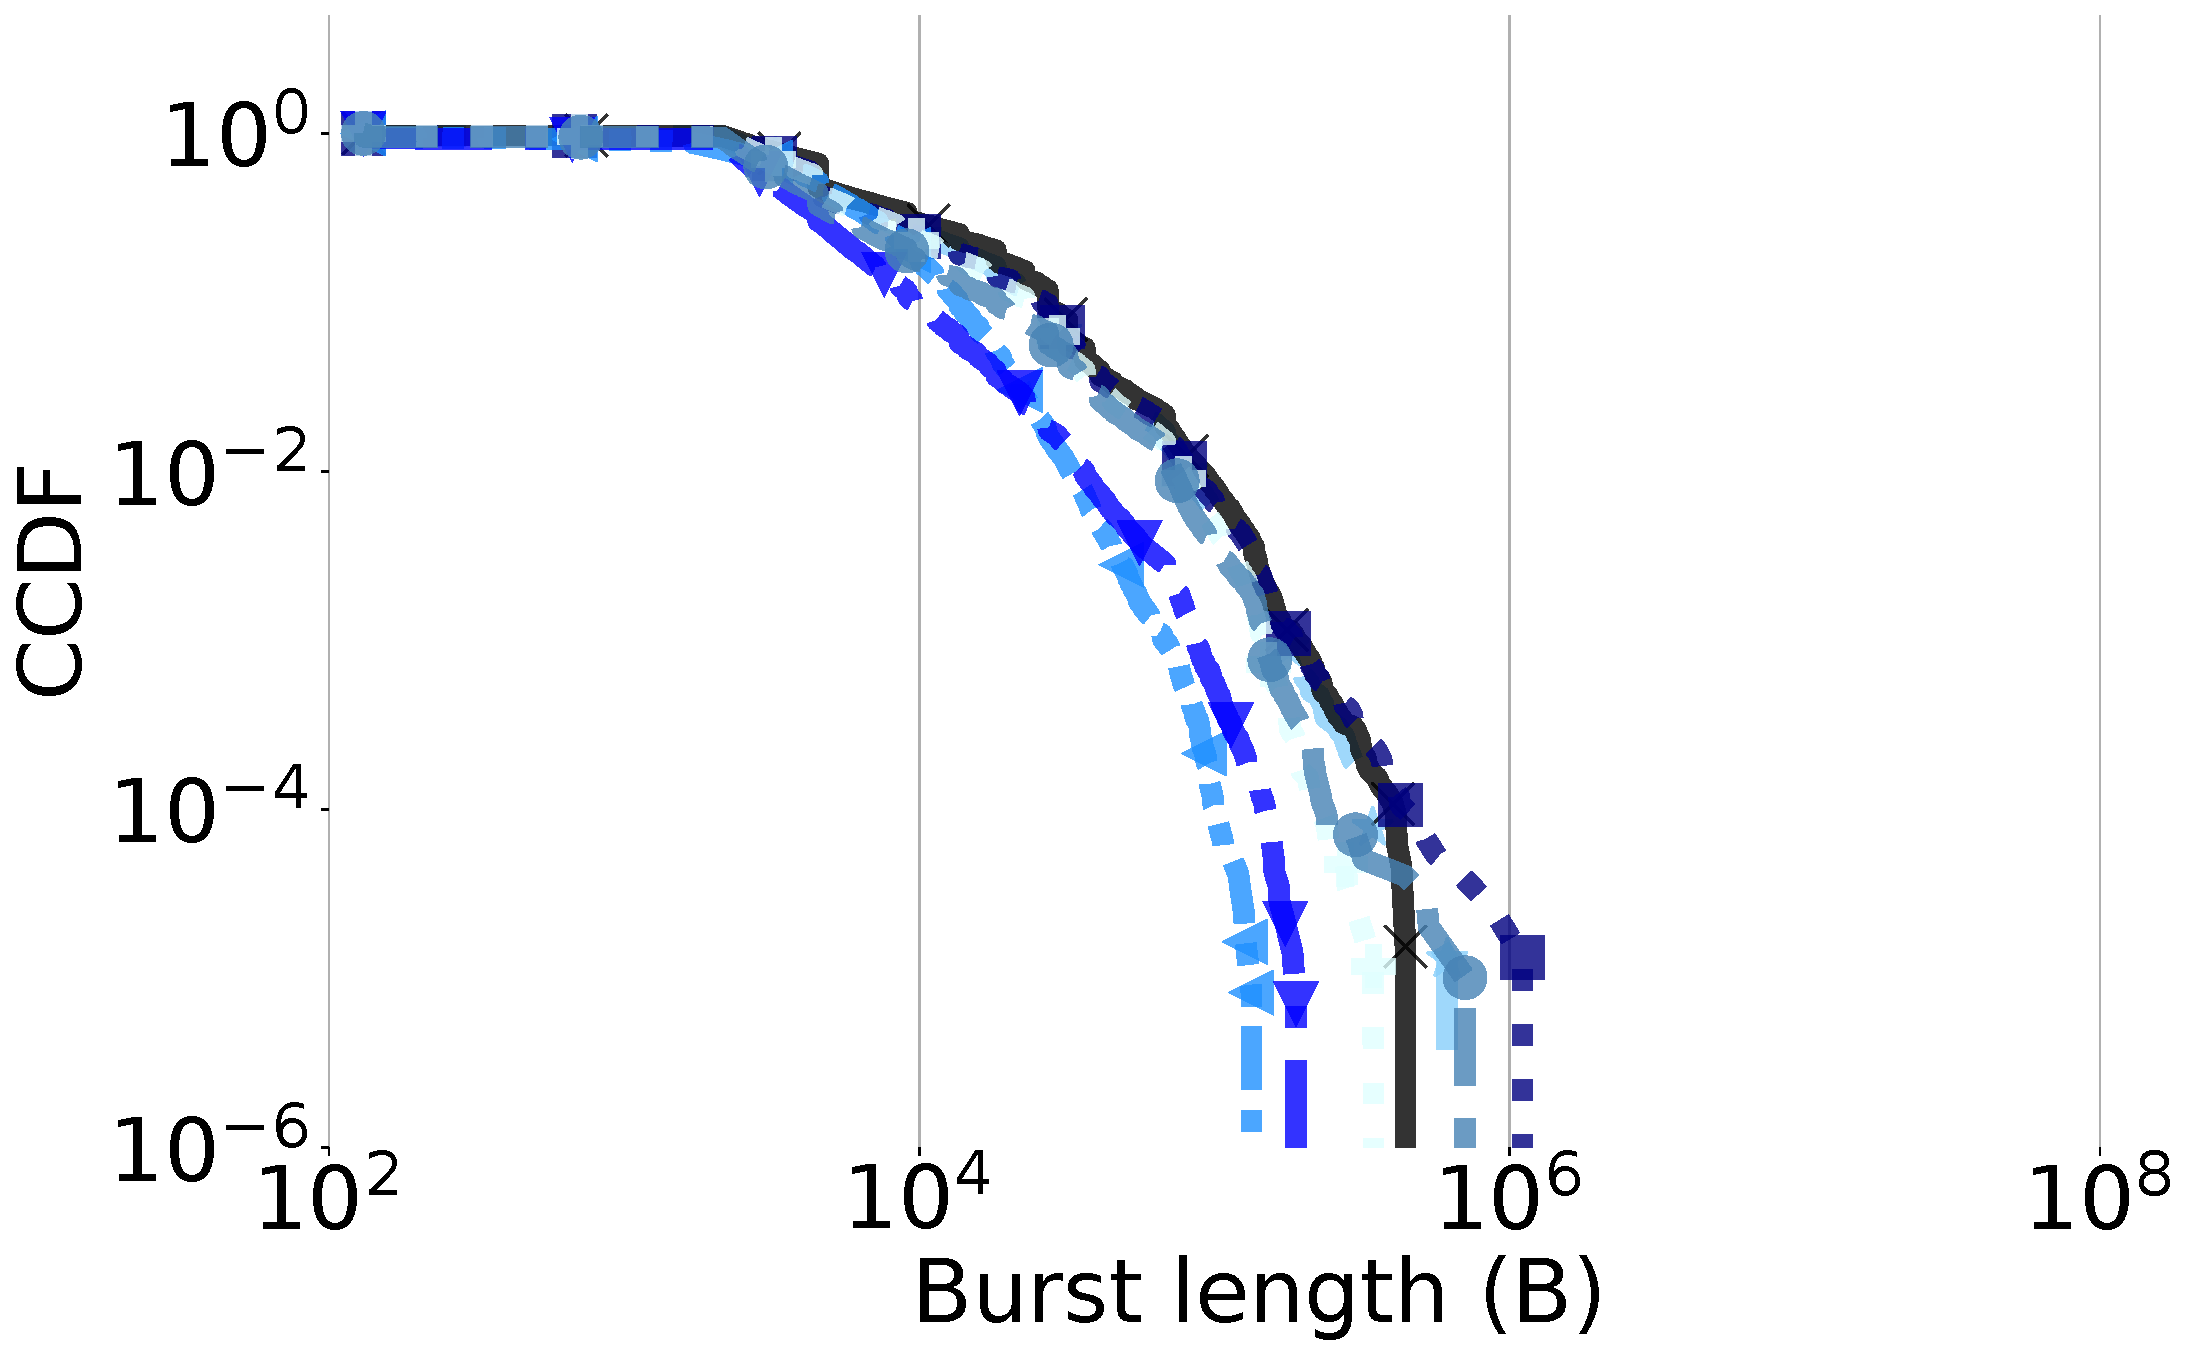
\includegraphics[width=1\linewidth]{figs/fileccdf_testbed.pdf}
    \caption{In-network microbursts}
	\label{fig:filecdf-testbed}
\end{subfigure}
\begin{subfigure}[t]{0.32\linewidth}
    \centering
    	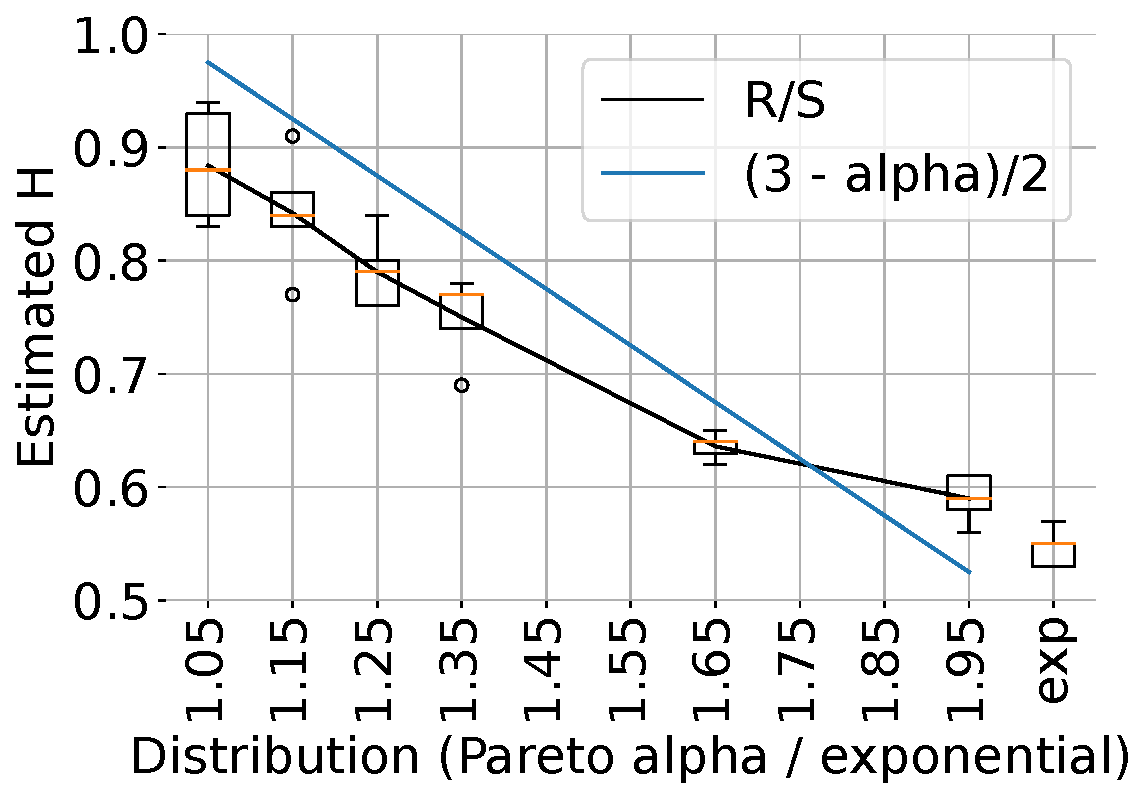
\includegraphics[width=1\linewidth]{figs/filehurst_sim.pdf}
    \caption{Simulation Hurst exp.}
	\label{fig:filehurst-sim}
\end{subfigure}
\begin{subfigure}[t]{0.32\linewidth}
    \centering
    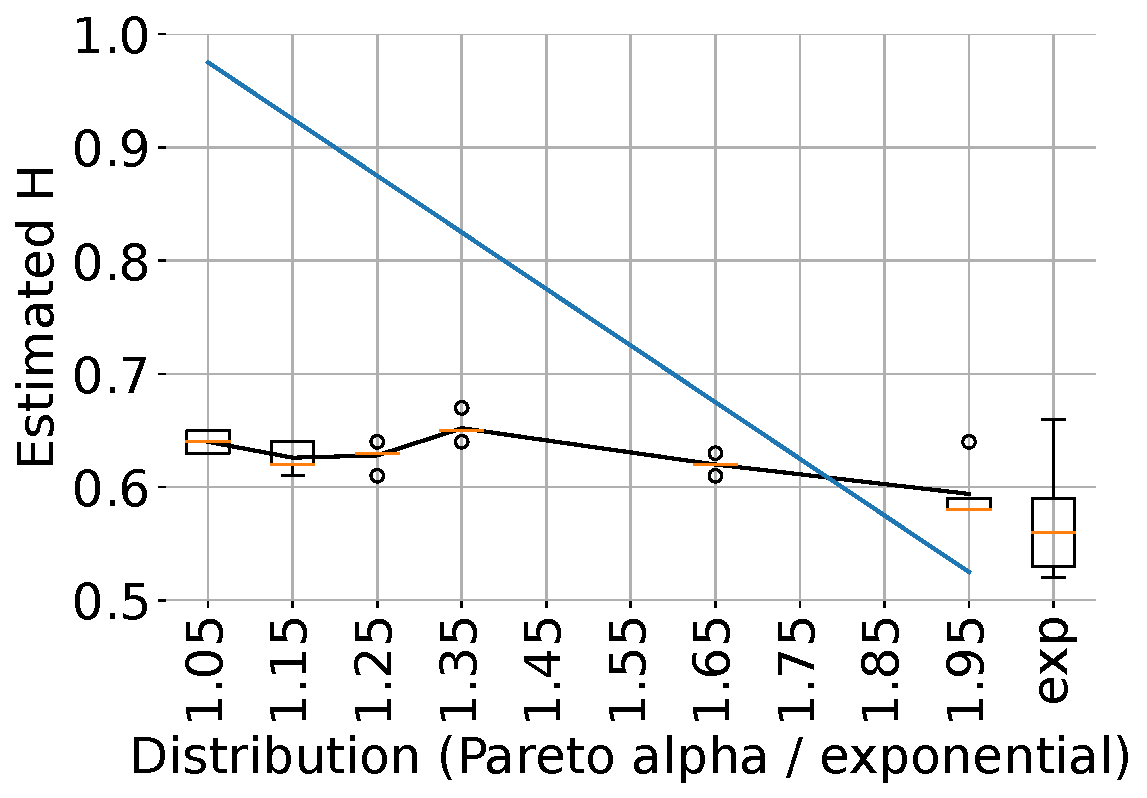
\includegraphics[width=1\linewidth]{figs/filehurst_ebpf_testbed.pdf}
    \caption{In-host Hurst exponents}
	\label{fig:fhurst-ebpf}
\end{subfigure}
\centering
\begin{subfigure}[t]{0.32\linewidth}
    \centering
    	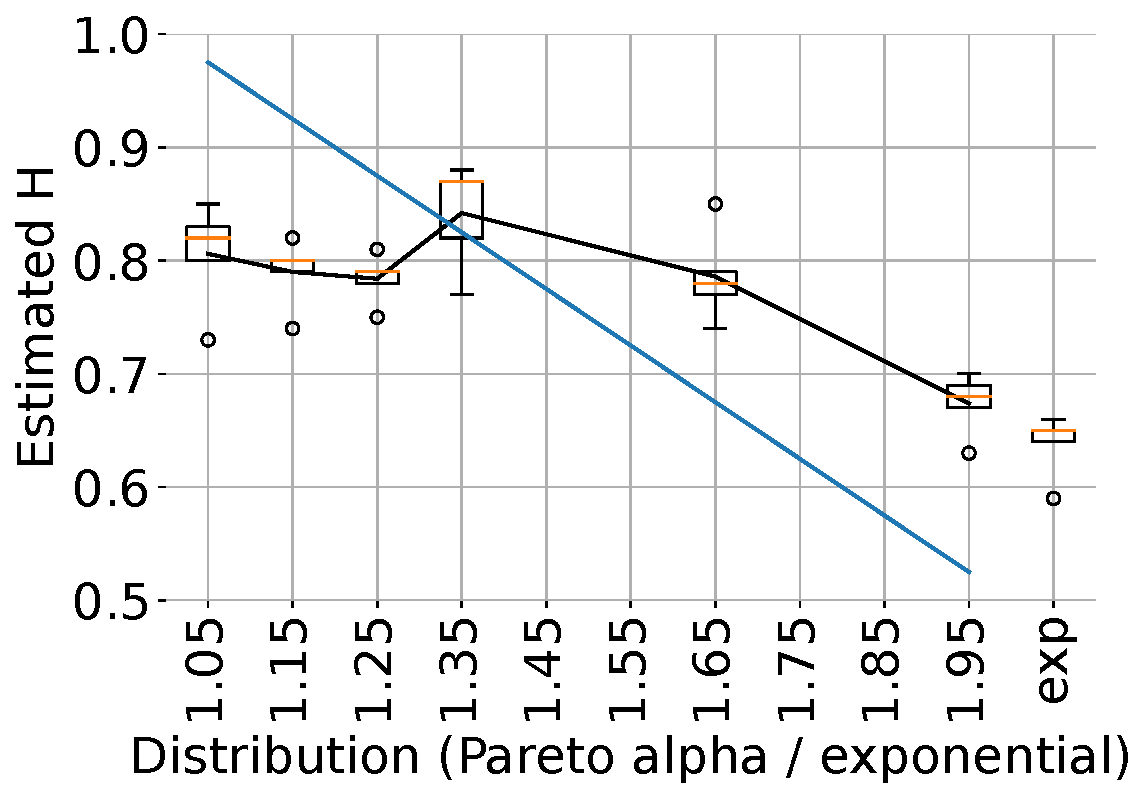
\includegraphics[width=1\linewidth]{figs/filehurst_testbed.pdf}
    \caption{In-network Hurst exp.}
	\label{fig:filehurst-testbed}
\end{subfigure}
 % \vspace{-2mm}
    \caption{\small{Microburst sizes and Hurst exponents of different synthetic workloads for simulated and testbed experiments are significantly different. 
    % The interference of host networking elements is visible in the difference between the three scenarios.
    }}
	\label{fig:filesize}
  % \vspace{-2mm}
\end{figure}

\subsection{Revisiting structural causality}
%Where does traffic burstiness come from? Is burstiness an artifact of application and workload internals, or is the host networking stack responsible for this temporal rise in traffic intensity at short time scales?
%To investigate, we run a network simulation, where 32 long-running TCP connections use Pareto and exponential flow size distributions depicted in Figure \ref{fig:filecdf-dist}. Flows are initiated exponentially and we set the distribution means in each case to make sure the offered load stays the same. We conduct all the simulations for five times in the OMNET \cite{omnet} simulator with a setup that imitates our physical testbed setting. According to \cite{filesize}, different $\alpha$ values for Pareto distributed flow sizes lead to different burstiness. Figure \ref{fig:filecdf-sim} testifies to the above claim. 
%While all synthetic flow size distributions have a mean of 4200KB, as Pareto $\alpha$ increases from 1.05 to 1.95, the heavy tail of the distribution is cut shorter and the size of bursts decreases accordingly. We observe that a light-tail distribution like exponential results in the lowest burstiness among all cases. The results in the CDF figure can also be interpreted by comparing the Hurst exponent estimates presented via the box-whisker plots in Figure \ref{fig:filehurst-sim}. 
%\erfan{Concretely, each box depicts the first and third quartiles of the estimated Hurst exponents for repeated simulation runs. The whiskers represent the upper and lower extremes, the circles are outlier points and the orange dashes present the mean values for Hurst estimates over multiple runs.}
%The trend in the rescaled-range estimates of Hurst exponents can be regressed to the (3$\alpha / 2$) line as we increase the $\alpha$ setting from 1.05 to 1.95.

%Next, we repeat the above scenario in a testbed, collecting the arrival timestamps both in the sending host and in the network. Figures \ref{fig:filecdf-testbed} and \ref{fig:filehurst-testbed} present the burst length distribution and Hurst estimates captured by Valinor-N in the network. Compared to the simulations, which lack the host network stack elements, Pareto $\alpha$ values that are lower than 1.95 result in almost the same amount of burstiness in the testbed. Only Pareto (1.95) and exponential cases are distinguishable since the p99 flow sizes in these two cases are 21KB and 18KB, respectively. Therefore, compared to the p99 flow size of 122KB for Pareto (1.05), they are less expected to produce trains of packets that form bursts. The trend in Hurst estimates also demonstrates that self-similarity does not follow the regressed (3$\alpha / 2$) line anymore.
%Finally, we report the in-host burstiness measurements of Valinor-H eBPF framework. The straight line between the boxes in Figure \ref{fig:fhurst-ebpf} suggests that the self-similarity of Pareto flows is further faded away as we remove the lower level components of the host networking stack from the picture (Valinor-H is placed before NIC processing in the stack). Compared to the in-network picture of burstiness, we observe that all the cases converge further to smaller H estimates (< 0.7). The burst length distributions in Figure \ref{fig:fccdf-ebpf} also conform to these findings.

Where does traffic burstiness come from?  
Prior work \cite{filesize, park1997effect, feldmann1999dynamics} shows that the heavy-tailed property of the flow size distribution directly determines link-level traffic self-similarity, a phenomenon that is sometimes referred to as \emph{structural causality}.  Heavy-tailed flow size distributions are shown to be the sufficient condition for generating scale-invariant burstiness and the network stack is shown to play a negligible role in self-similarity \cite{filesize, feldmann1999dynamics}. 
%
For instance, for traffic generated by TCP Reno for a heavy-tailed Pareto file size distribution with the shape parameter $\alpha$, there exists an almost linear relation between $H$ and $\alpha$: the estimated $H$ is close to $(3-\alpha)/2$.\footnote{The $H=(3-\alpha)/2$ relation shows the values of $H$ predicted by the a theoretical ON/OFF model in the idealized case corresponding to a fractional Gaussian noise process with independent traffic sources with constant ON/OFF amplitude \cite{park1997effect}. This captures an ideal self-similar process.} 
%with a slightly lower slope, an offset below the idealized line for $\alpha$ close to 1 (more heavy-tailed), and above the line for $\alpha$ close to 2 (less heavy-tailed).
Heavier tailed distributions (i.e., $\alpha$ close to 1) are more strongly self-similar ($H$ closer to 1). The self-similarity of traffic with heavy-tailed flow sizes is in contrast to the lack of correlation structures for short-tailed flow size distributions such as an exponential distribution ($H$ close to 0.5).

We first replicate this result using OMNET \cite{omnet}, an extensively used simulator \cite{homa,conga,fatpaths}, and observe an almost linear relation between $\alpha$ and $H$---consistent with the findings of prior work \cite{filesize}, the estimated $H$ values closely track the $(3-\alpha)/2$ line. In a setup where the two simulated servers are connected via a network switch, we establish 32 long-running TCP connections and use Pareto and exponential flow size distributions (Figure \ref{fig:filecdf-dist} shows the flow size distributions). To achieve a target offered load of 6 Gbps, flows are initiated exponentially with a mean interarrival time of 87$\mu$s. We repeat each experiment five times. In the box and whisker plots, each box depicts the $1^{st}$ and $3^{rd}$ quartiles, the whiskers represent the upper and lower extremes, the circles are outlier points, and the orange dashes show the median Hurst estimates. Figure \ref{fig:filehurst-sim} shows that heavy-tailed flow size distributions generate self-similar traffic. Figure \ref{fig:filecdf-sim} shows that these distributions also result in larger microbursts with heavier tails.

Next, we repeat the above scenario in a testbed, using Valinor to analyze burstiness after the software stack and on the wire. Using Valinor-H for in-host analysis, we observe that the impact of the heavy-tailed distributions on self-similarity is barely visible at this stage with distributions with varying $\alpha$ parameters behaving similarly and close to a light-tail exponential distribution (Figure \ref{fig:fhurst-ebpf}), e.g., the software stack greatly diminishes the degree of self-similarity of heavy-tailed Pareto distribution with $\alpha=1.05$ from $H=0.88$ in the simulations (Figure \ref{fig:filehurst-sim}) to $H=0.64$ at the eBPF hook (Figure \ref{fig:fhurst-ebpf}). We observe a similar effect on the microburst size distributions that are much more similar across different workloads and have shorter tails (Figure \ref{fig:fccdf-ebpf}).

We next use Valinor-N for analyzing traffic as observed on the wire. The patterns again change in interesting and non-uniform ways. Similar to in-host measurements, the in-network measurements indicate that the influence of flow size on self-similarity is lower than the simulated experiments, e.g., $H=0.80$ and $H=0.78$ for $\alpha=1.05$ and $\alpha=1.65$, respectively, on the wire in the testbed experiments compared to $H=0.88$ and $H=0.63$ for the same workloads in the simulated experiments (Figure \ref{fig:filehurst-testbed}). The more amplified long-range burstiness in the network compared to in-host experiments is due to the intervention of driver and NIC functions (such as segmentation offloading scheduling) that reside below Valinor-H. We investigate the roles of these functions in \S\ref{sec:sources}. 
%
Figure \ref{fig:filecdf-testbed} shows that the flow size distribution has a relatively subdued impact on the ultimate size of microbursts on the wire once the traffic traverses the host networking stack.

\paragraph{Summary:} The shape of the traffic in the testbed experiments (in-network and in-host) is substantially different compared to the simulated experiments with identical setups. This suggests that host networking elements (e.g., qdiscs, process schedulers, and NIC schedulers, not modeled in common simulators) alter burstiness.

\begin{figure}[t]
\centering
\begin{subfigure}[t]{0.40\linewidth}
    \centering
    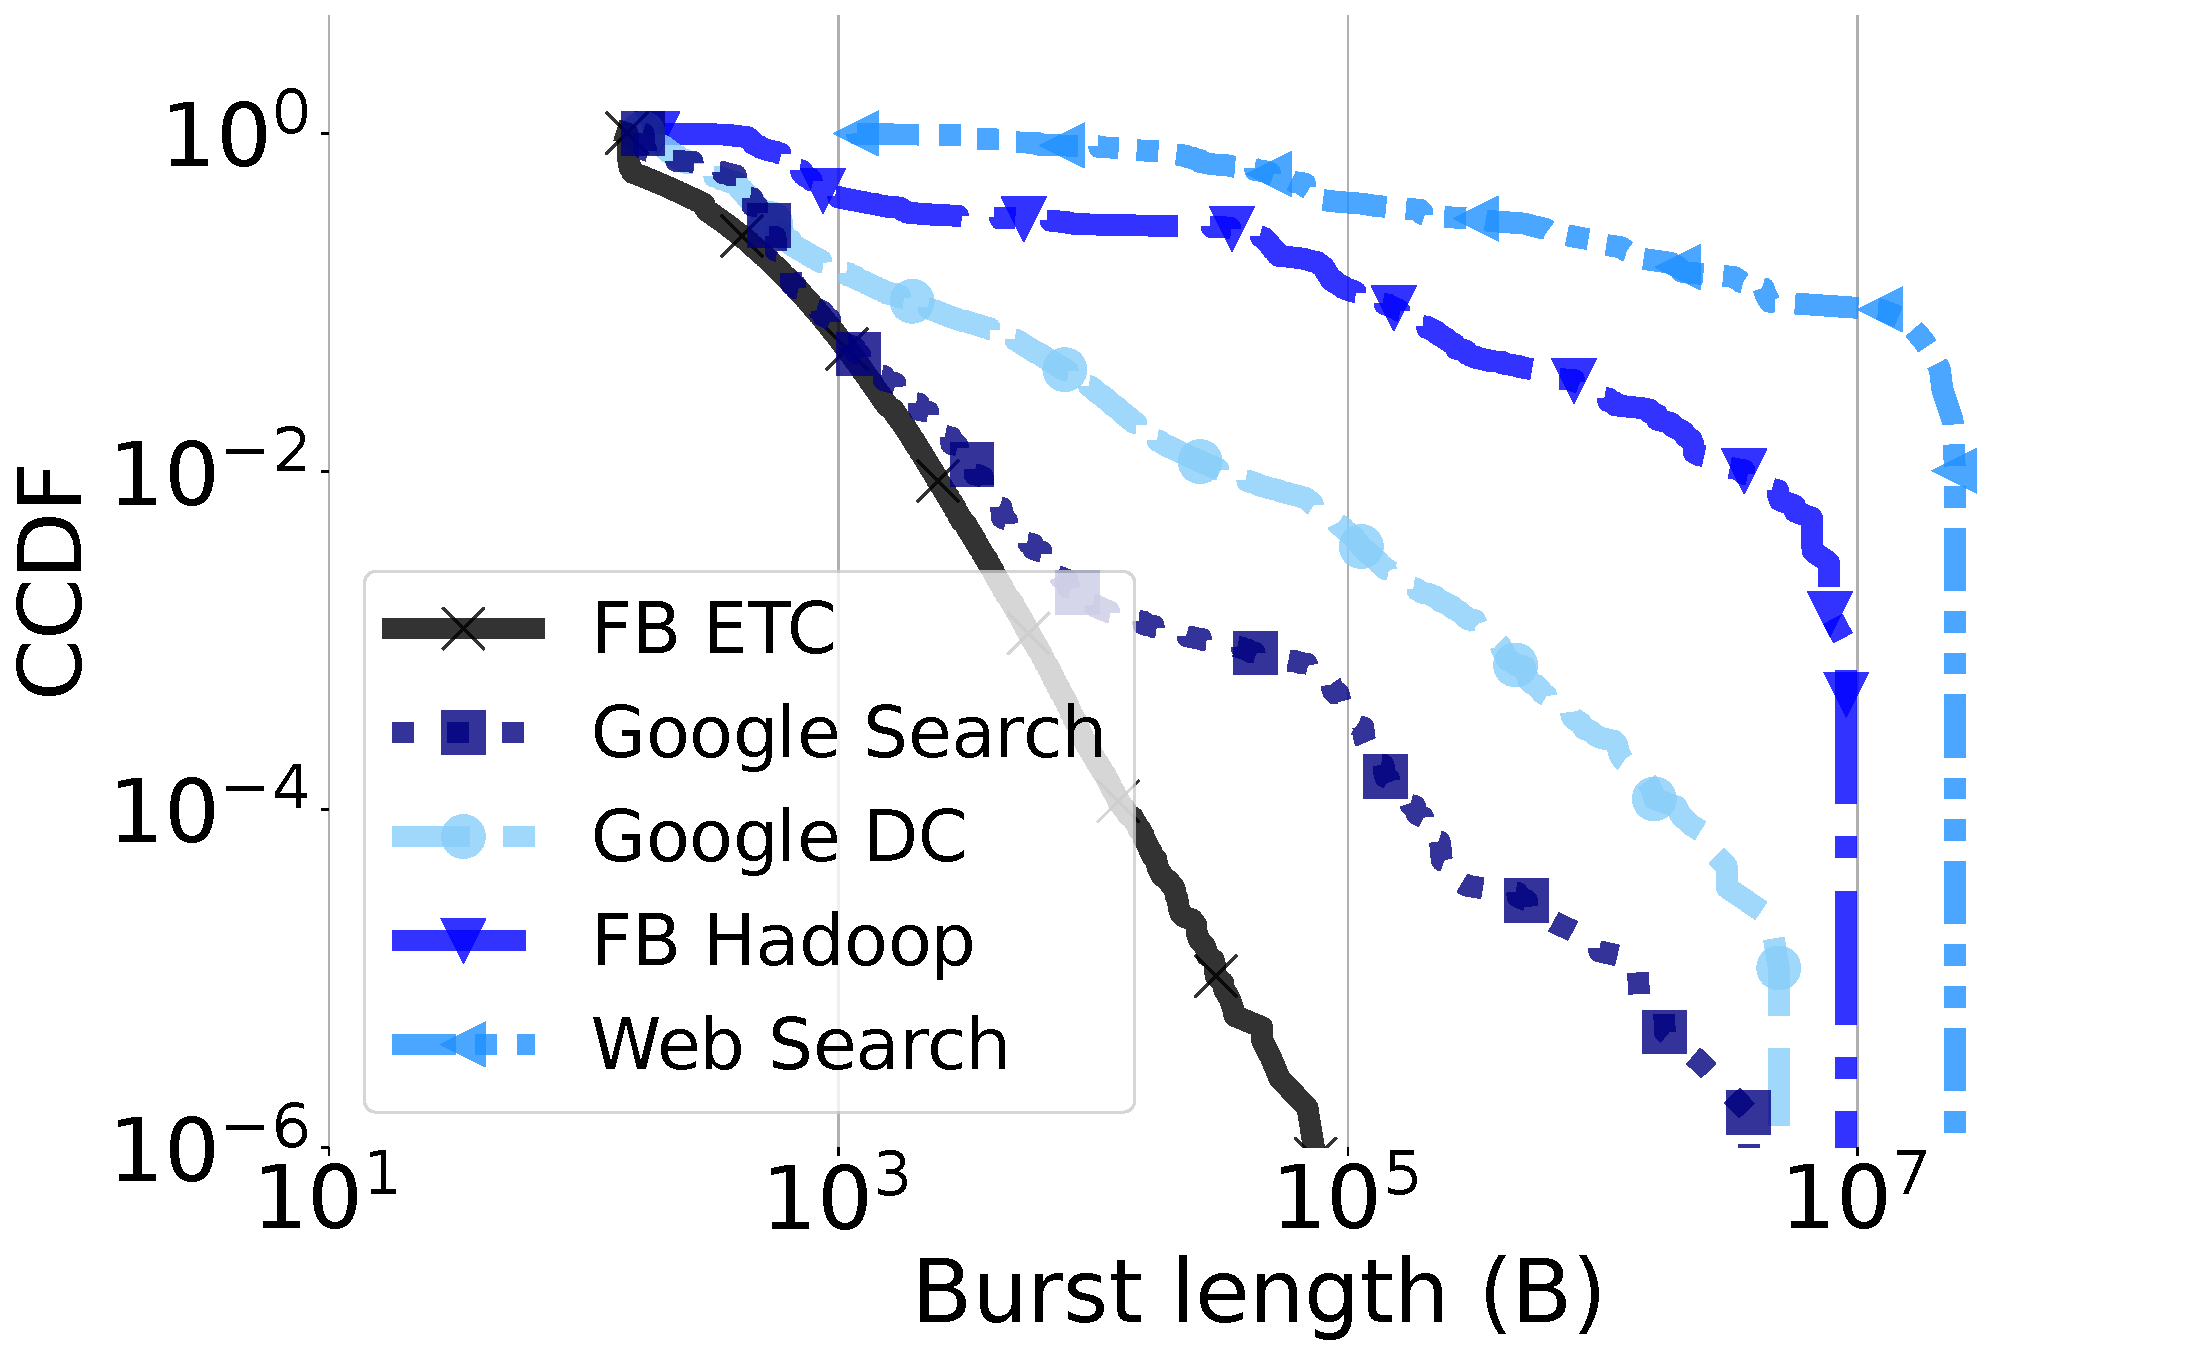
\includegraphics[width=1\linewidth]{figs/wccdf_sim.pdf}
    \caption{Simulation microburst sizes}
	\label{fig:wcdf-sim}
\end{subfigure}
\begin{subfigure}[t]{0.40\linewidth}
    \centering
    	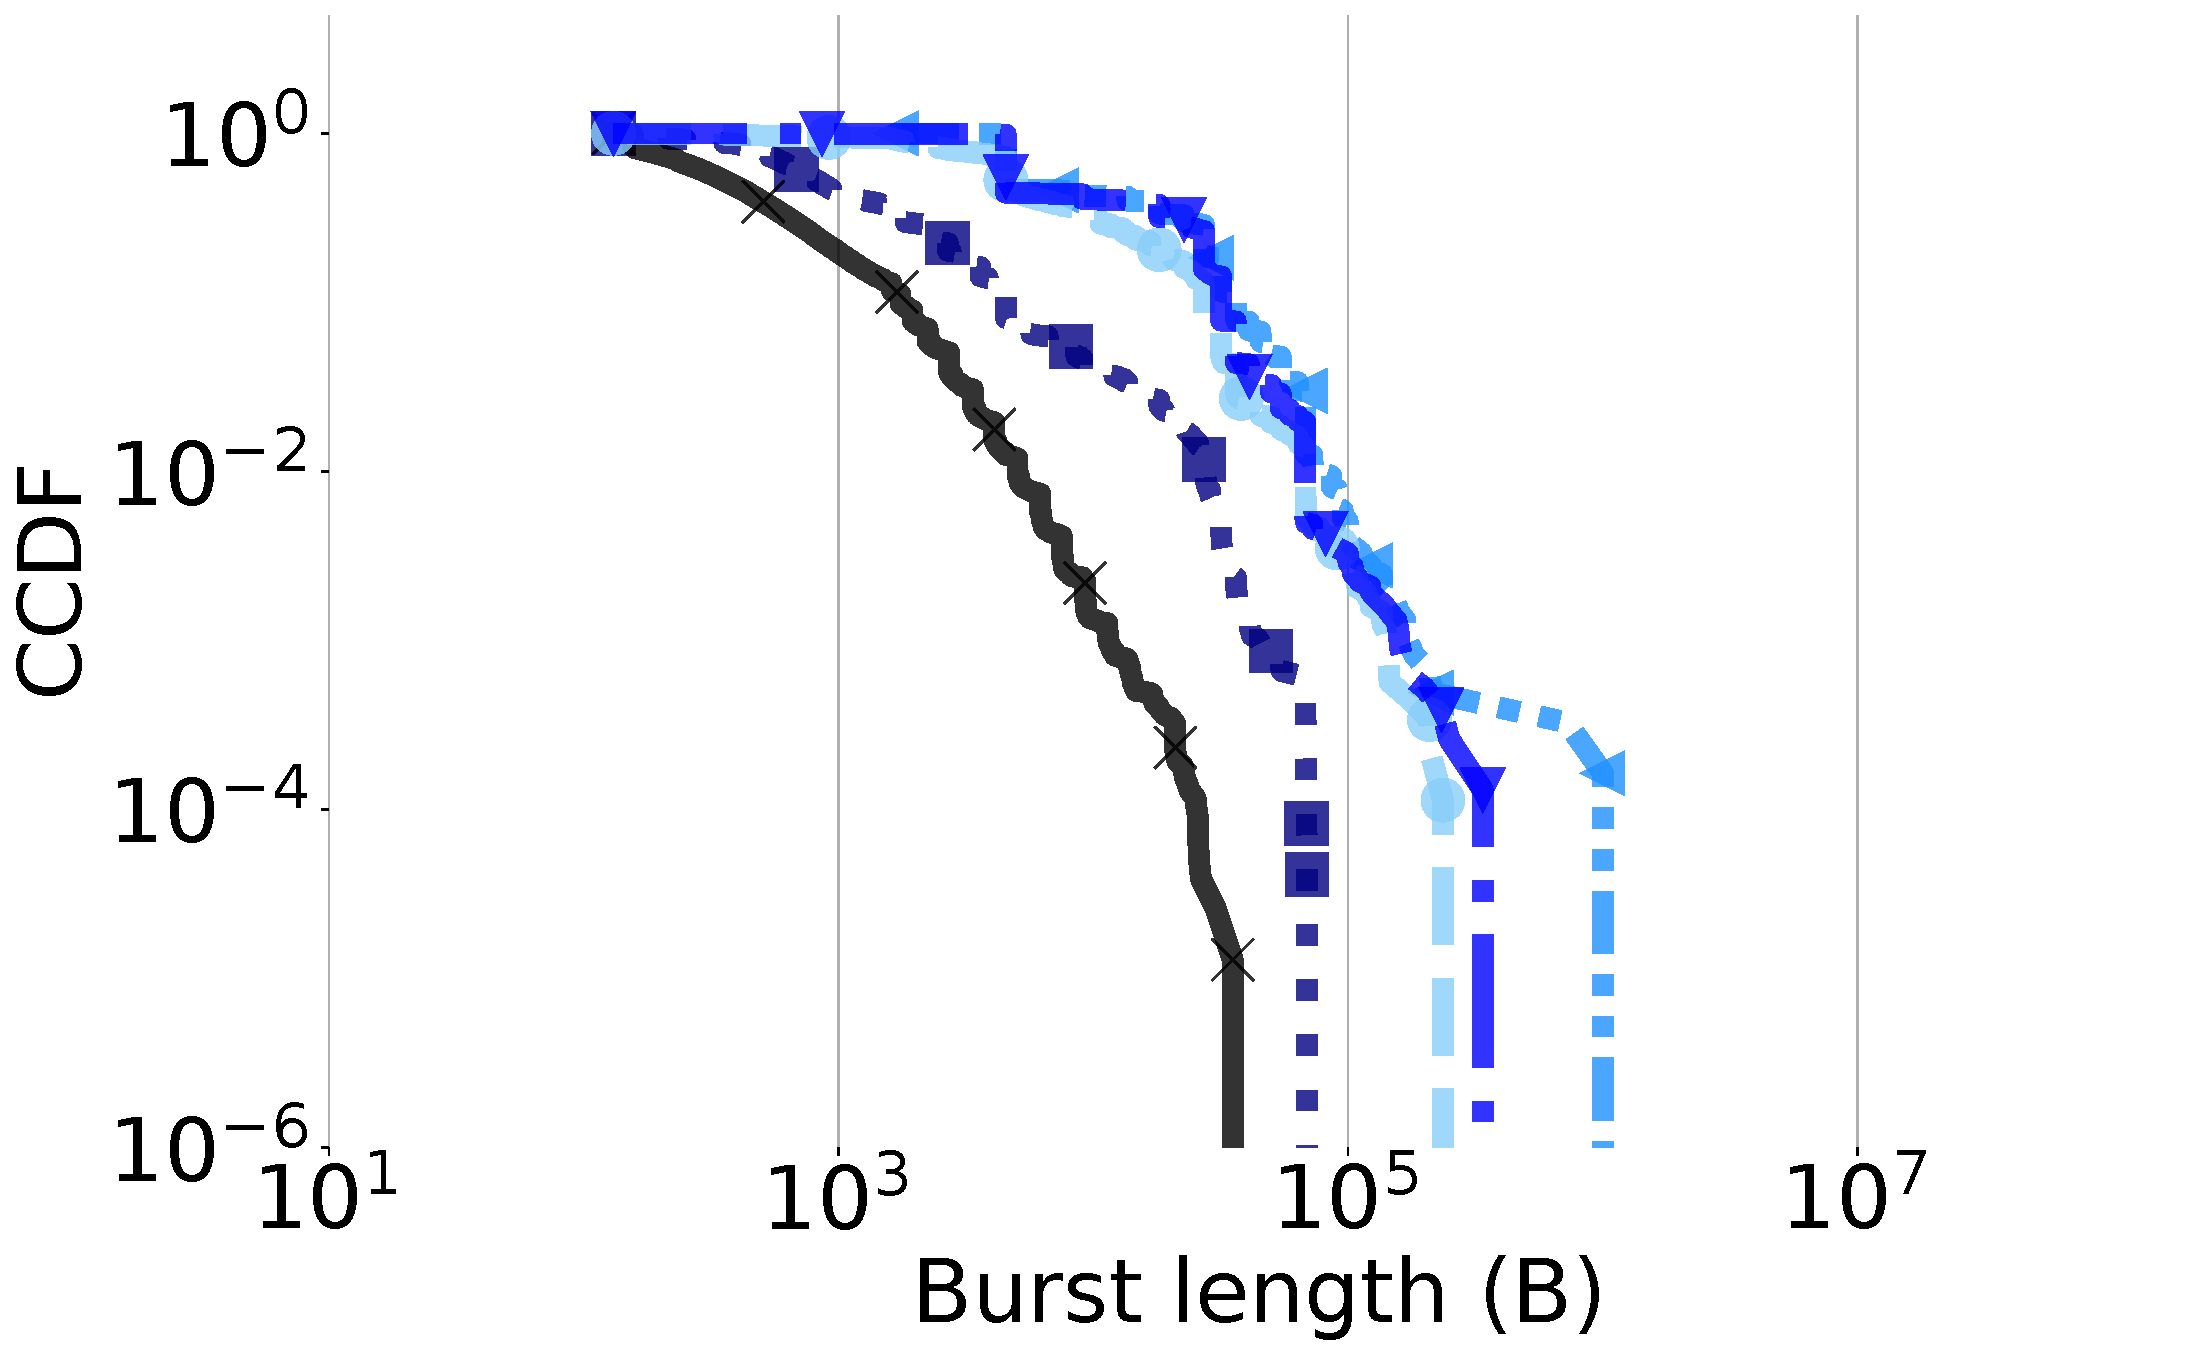
\includegraphics[width=1\linewidth]{figs/wccdf_testbed.pdf}
    \caption{In-network microburst sizes}
	\label{fig:wcdf-testbed}
\end{subfigure}
\begin{subfigure}[t]{0.40\linewidth}
    \centering
    	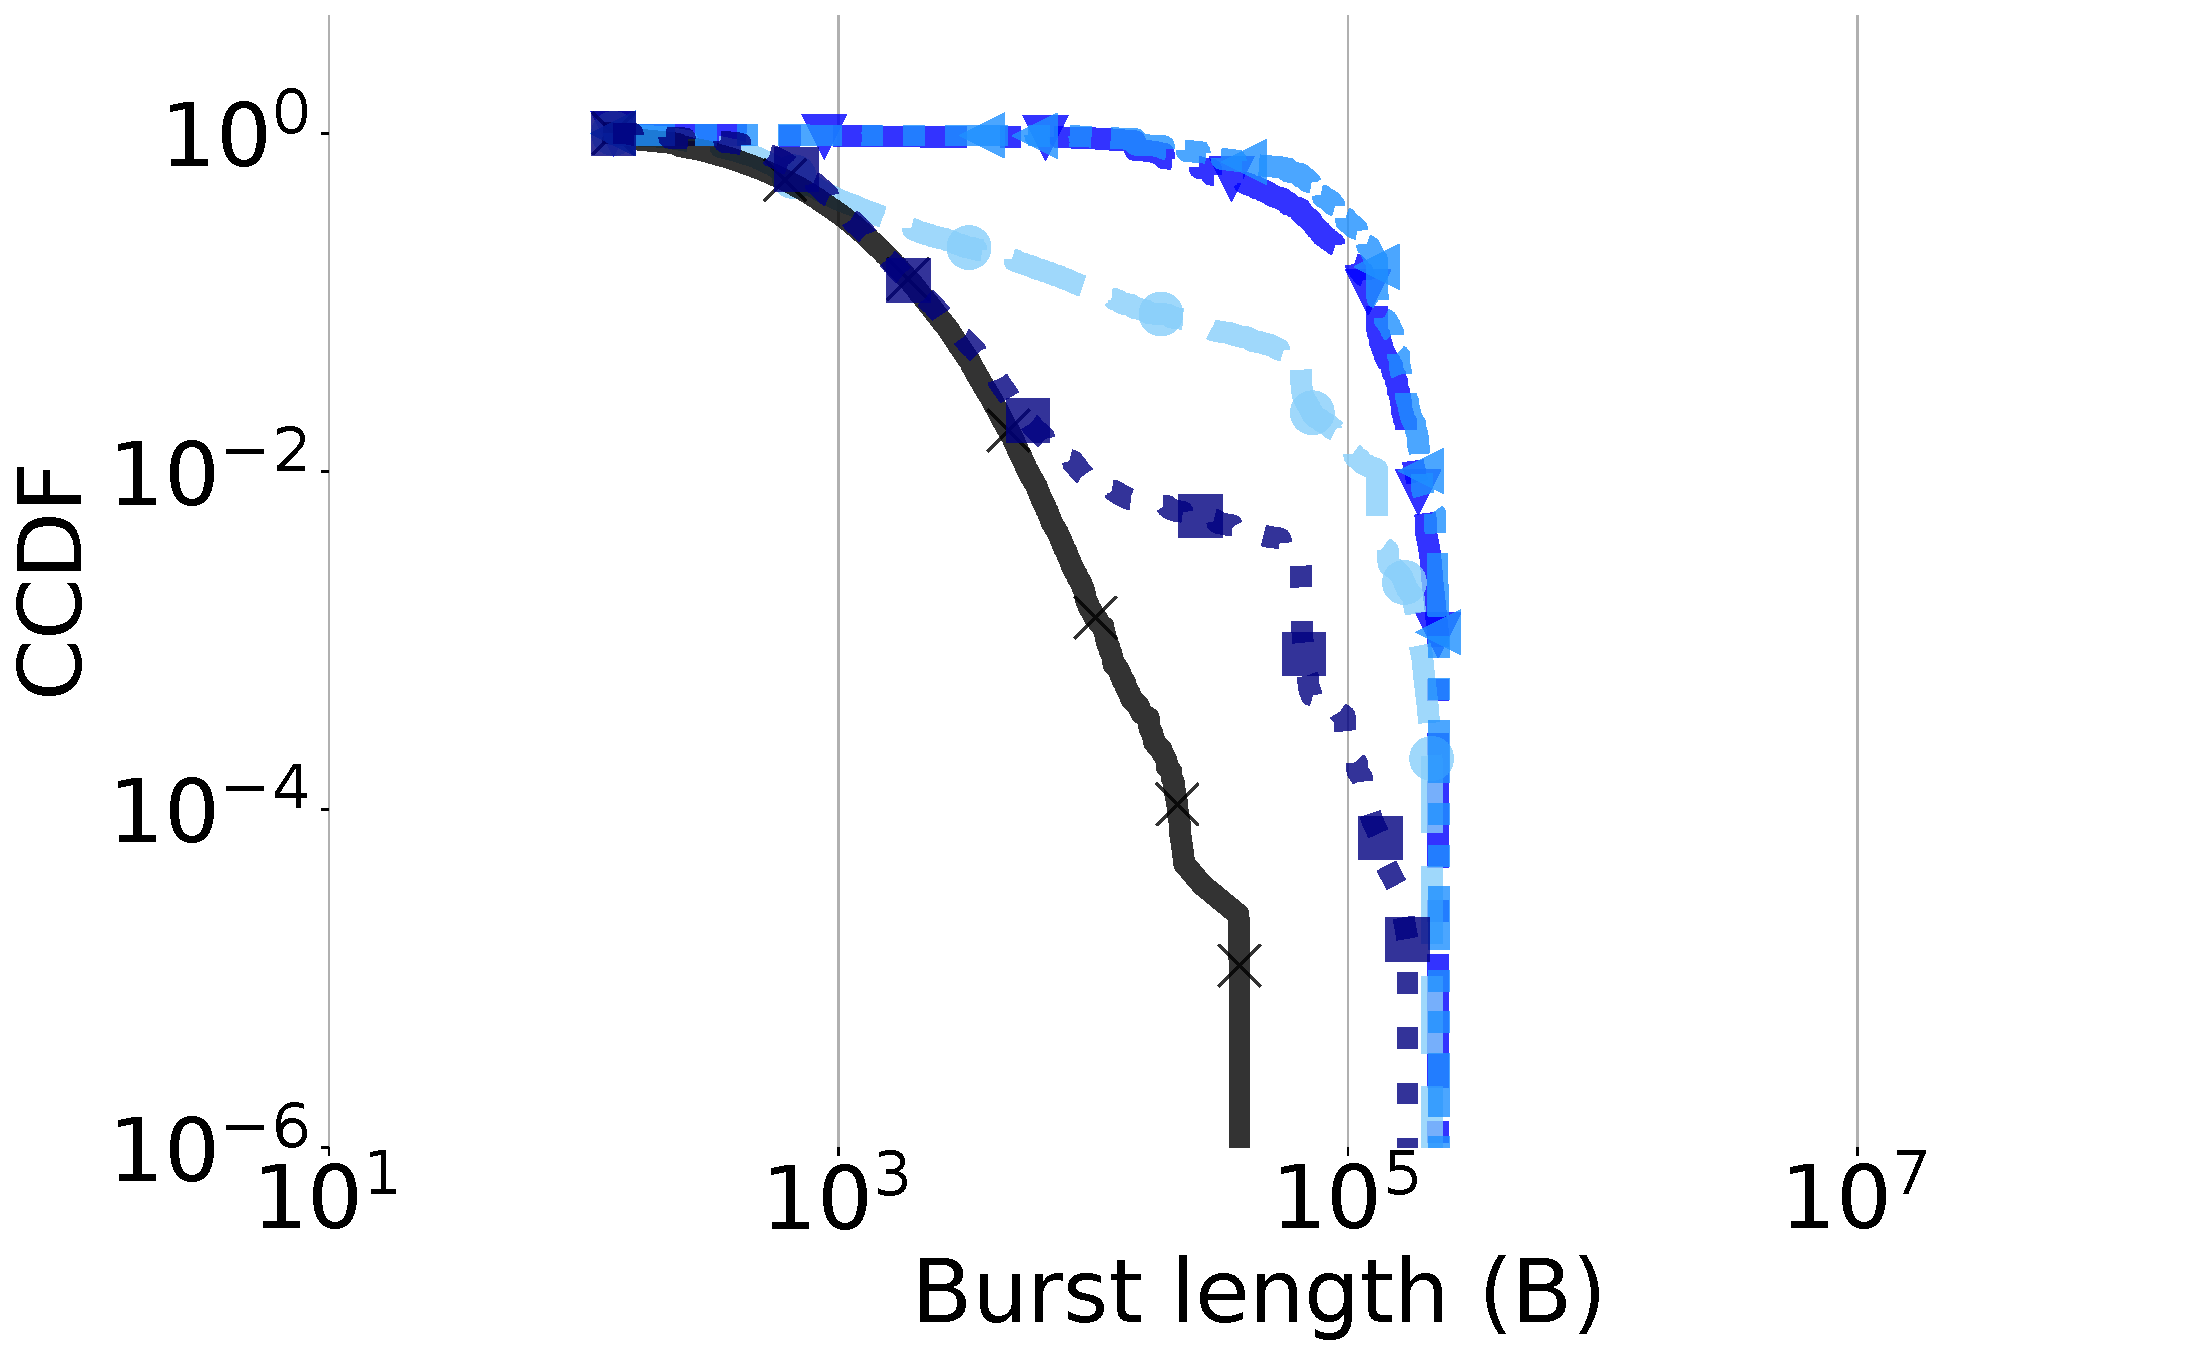
\includegraphics[width=1\linewidth]{figs/wccdf_ebpf_testbed.pdf}
    \caption{In-host microburst sizes}
	\label{fig:fwccdf-ebpf}
\end{subfigure}
\begin{subfigure}[t]{0.36\linewidth}
    \centering
    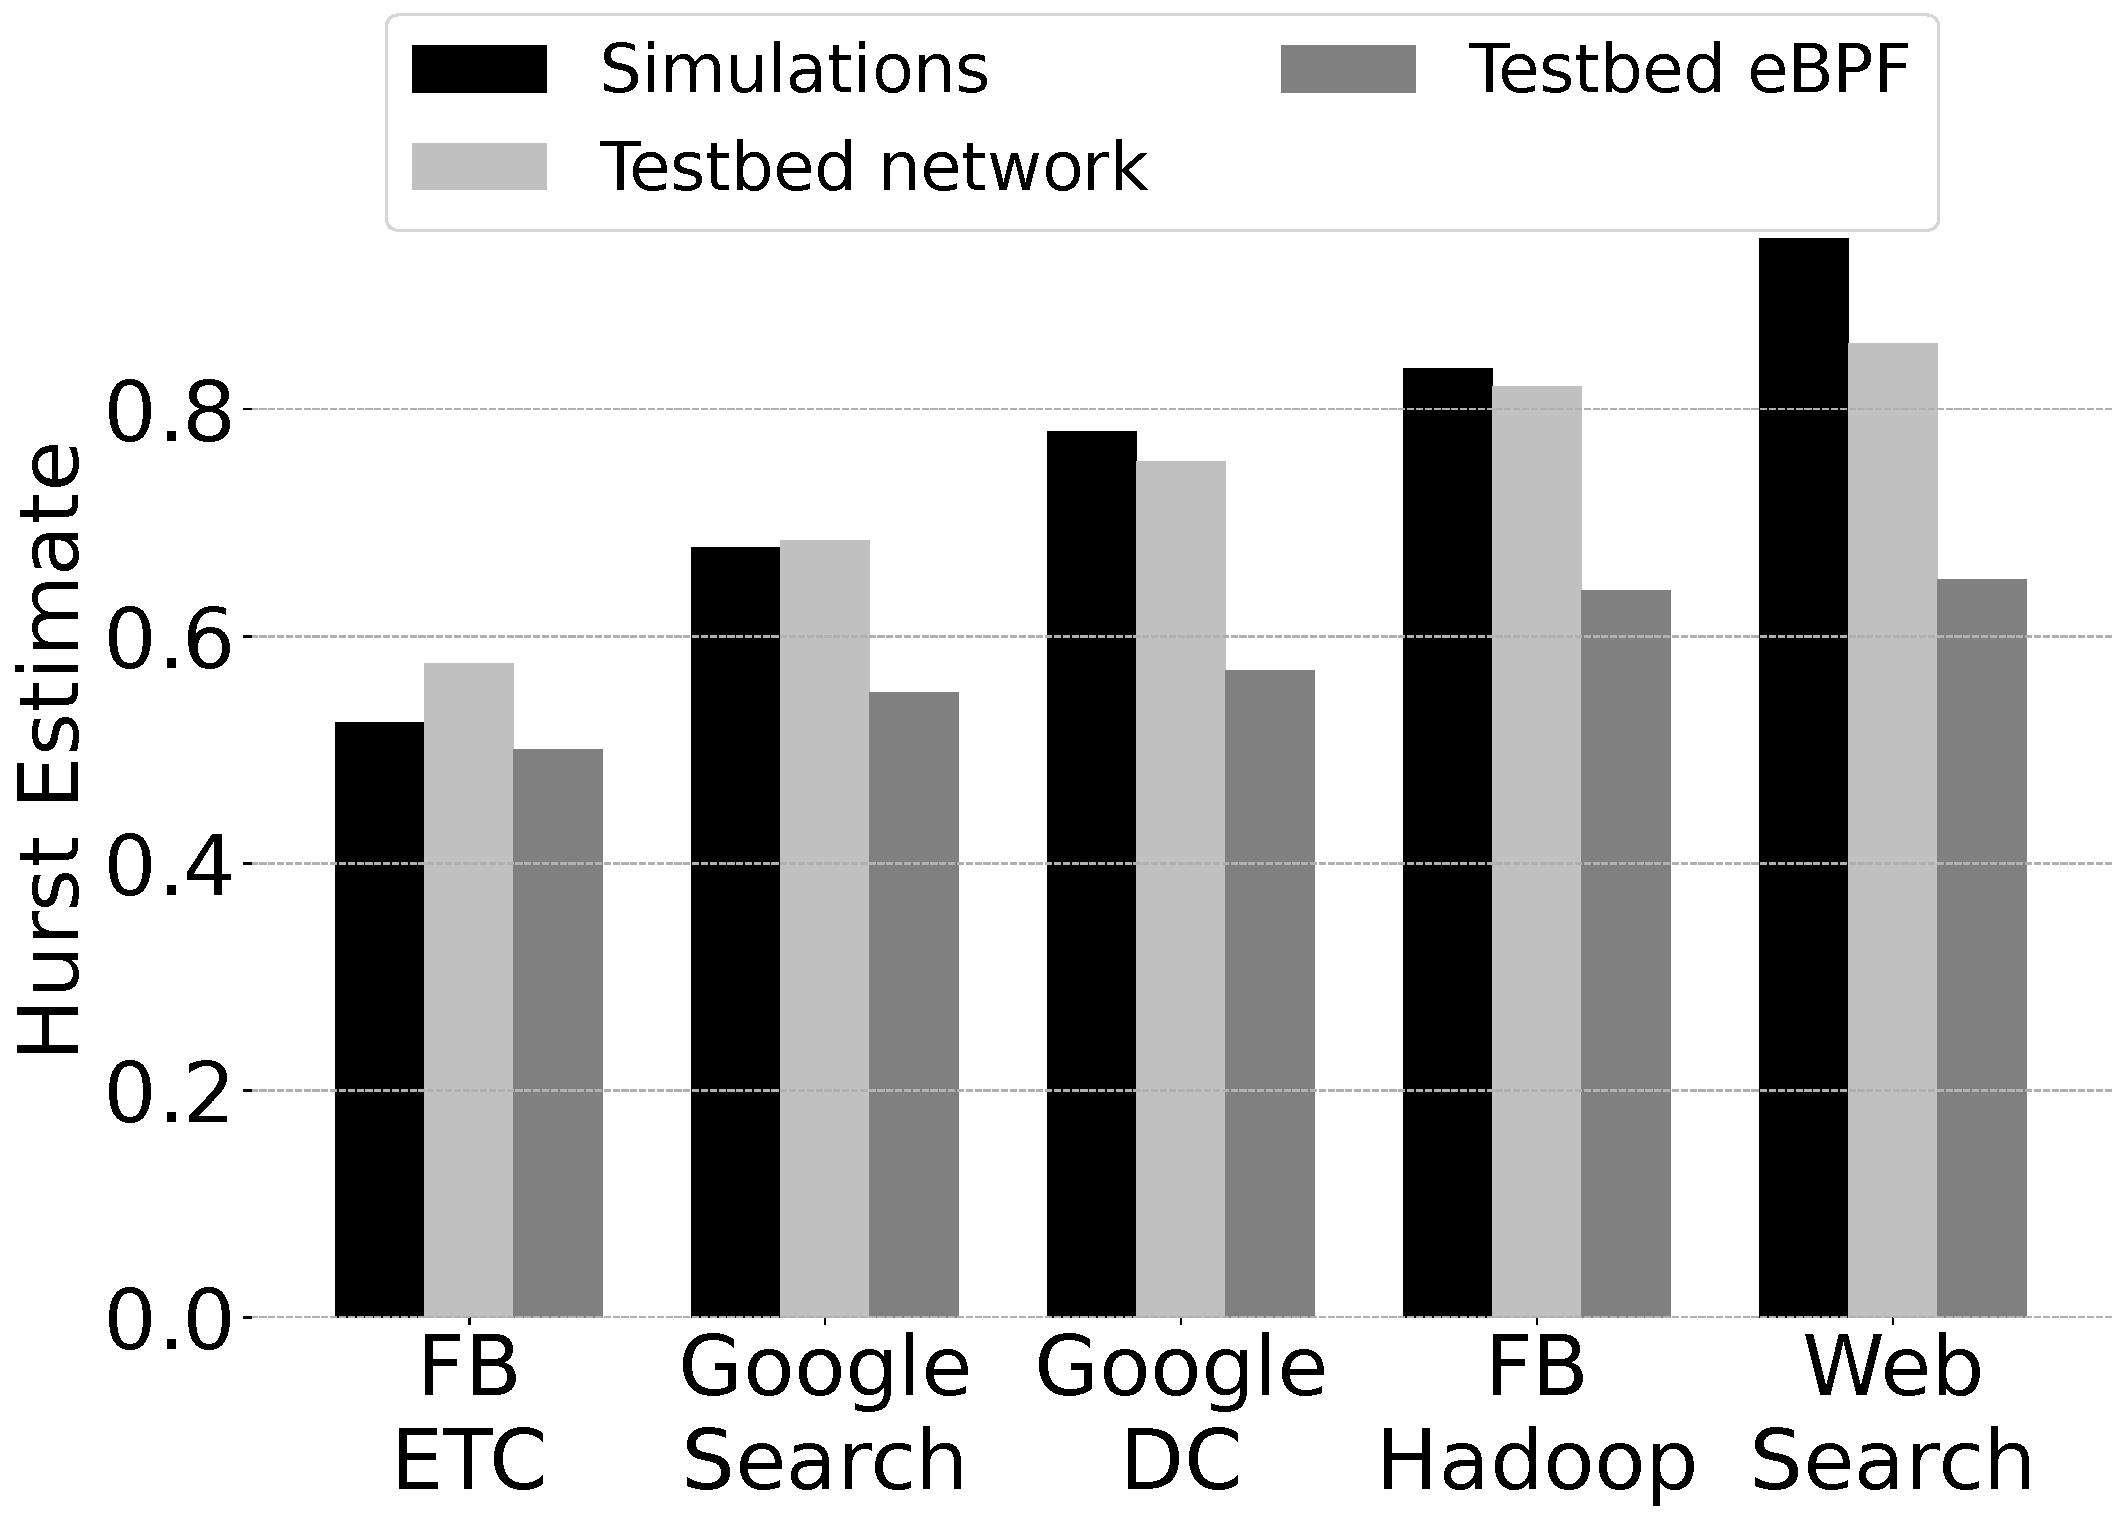
\includegraphics[width=1\linewidth]{figs/w_ebpf_hurst_bar.pdf}
    \caption{Estimated Hurst exponents}
	\label{fig:whurst-ebpf}
\end{subfigure}

    \caption{\small{
    Self-similarity and microburst sizes vary across workloads and between testbed and simulation results. Positioned before the NIC, Valinor-H captures a smoother snapshot of traffic than in-network measurements.
    }}
	\label{fig:traces}
 \vspace{-5mm}
\end{figure}

% \vspace{-2mm}
\subsection{Impact of workloads}
Next, we repeat the above experiments (using both the simulator and the testbed) by replaying the  traces of five classes of workloads from \cite{homa}: (1) Facebook's ETC workload,  (2) Google search workload, (3) Google's aggregated internal data center workload, (4) Facebook's Hadoop workload, (5) DCTCP's web search workload \cite{dctcp}.
Figure \ref{fig:trace-ccdf} shows the flow size distributions of these traces. 
Similar to the previous experiments, in simulations, there exists a direct correlation between the flow size distributions, self-similarity, and the burst lengths (Figure \ref{fig:traces}). In the testbed, however, the difference in burst lengths starts to fade away as host networking components come into play.
%
%Nonetheless, both Valinor-H and Valinor-N are able to capture the differences in traffic burstiness for the five traces of choice. 
We also observe that the scaling behavior varies substantially across different workloads and between the simulated and testbed experiments.
Hurst coefficients are larger for the more heavy-tailed distributions in the network but mostly homogeneous before reaching the driver.
For example, the self-similarity estimates for the ETC workload (p99$^{th}$ flow size = 1.8 KB), the Google DC workload (p99$^{th}$ flow size = 31 KB), and the web search workload (p99$^{th}$ flow size = 27 MB) are 0.57, 0.75, and 0.85, respectively for in-network measurements and 0.50, 0.57, and 0.65, respectively for in-host measurements.
%, all capturing the positive correlation between the workload size and its burstiness.
%The next mission is indeed discovering the role of host networking internals on traffic burstiness. In the following sections, we attempt to provide more insights.

\begin{figure}[t]
\centering
    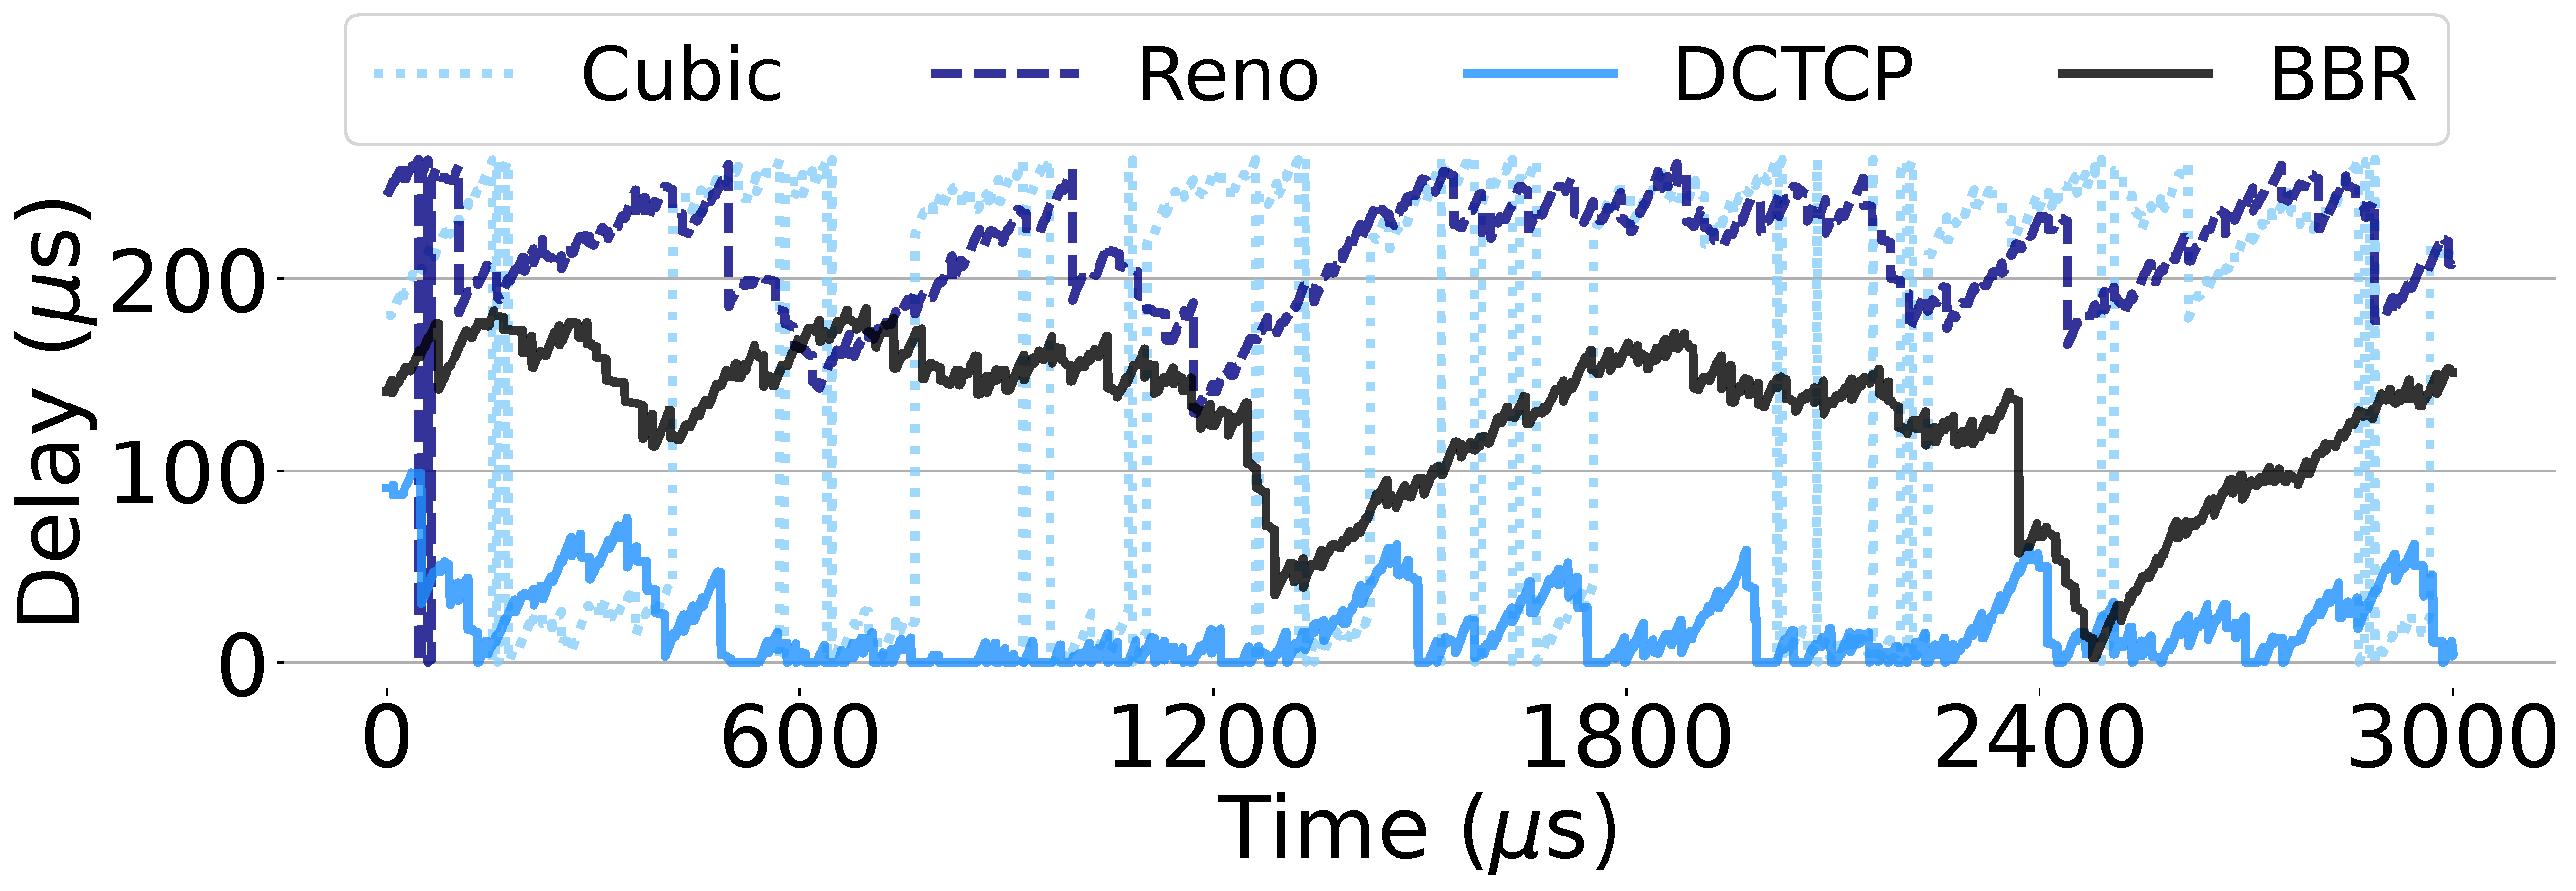
\includegraphics[width=0.8\linewidth]{figs/buffer_size.pdf}
    % \vspace{-6mm}
    \caption{\small{Buffer occupancy under Incast captured by Valinor-N}}
	\label{fig:transport-queue}
 \vspace{-2mm}
\end{figure}
% \vspace{5mm}
\begin{figure}[t]
\centering   
    \vspace{3mm}
    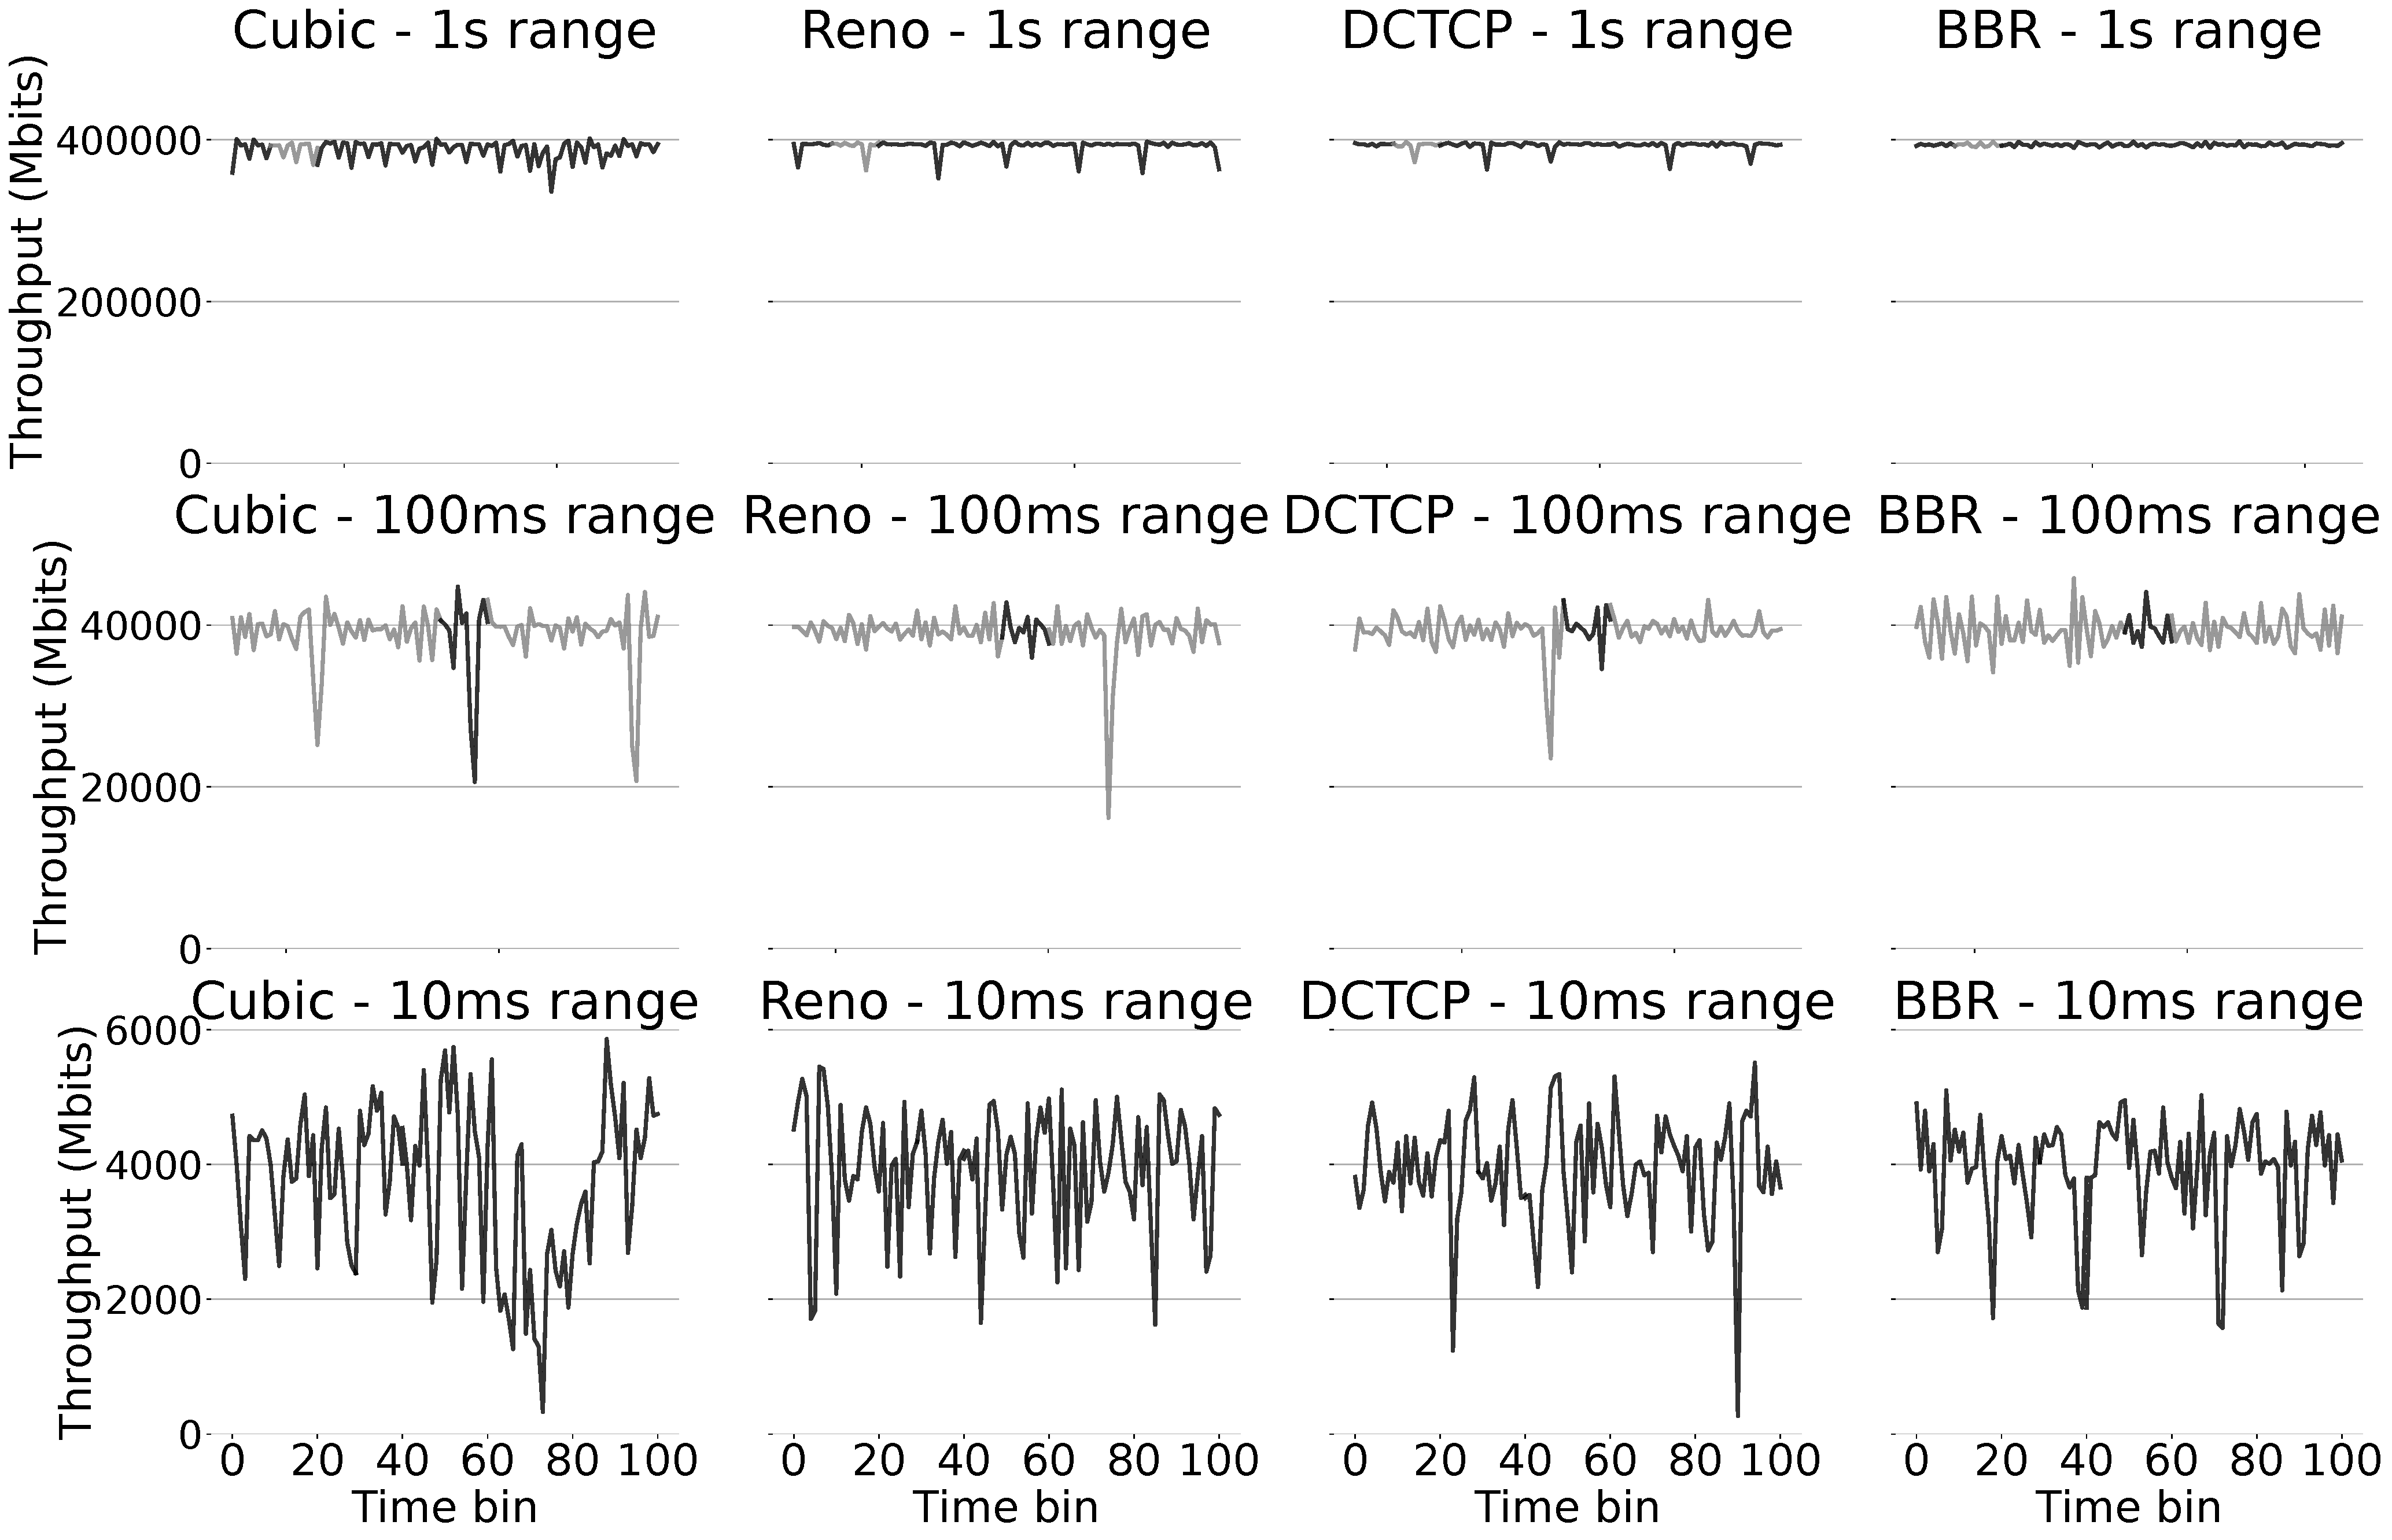
\includegraphics[width=0.85\linewidth]{figs/incast_byte_time_series.pdf}
    % \vspace{-2mm}
    \caption{\small{Timeseries of packet arrivals show that burstiness (at both short and long timescales) varies significantly across transport protocols.}}
	\label{fig:transport-ts}
     \vspace{-2mm}
\end{figure}

\begin{figure}[t]
\begin{minipage}[b]{0.49\textwidth}
    \centering
    	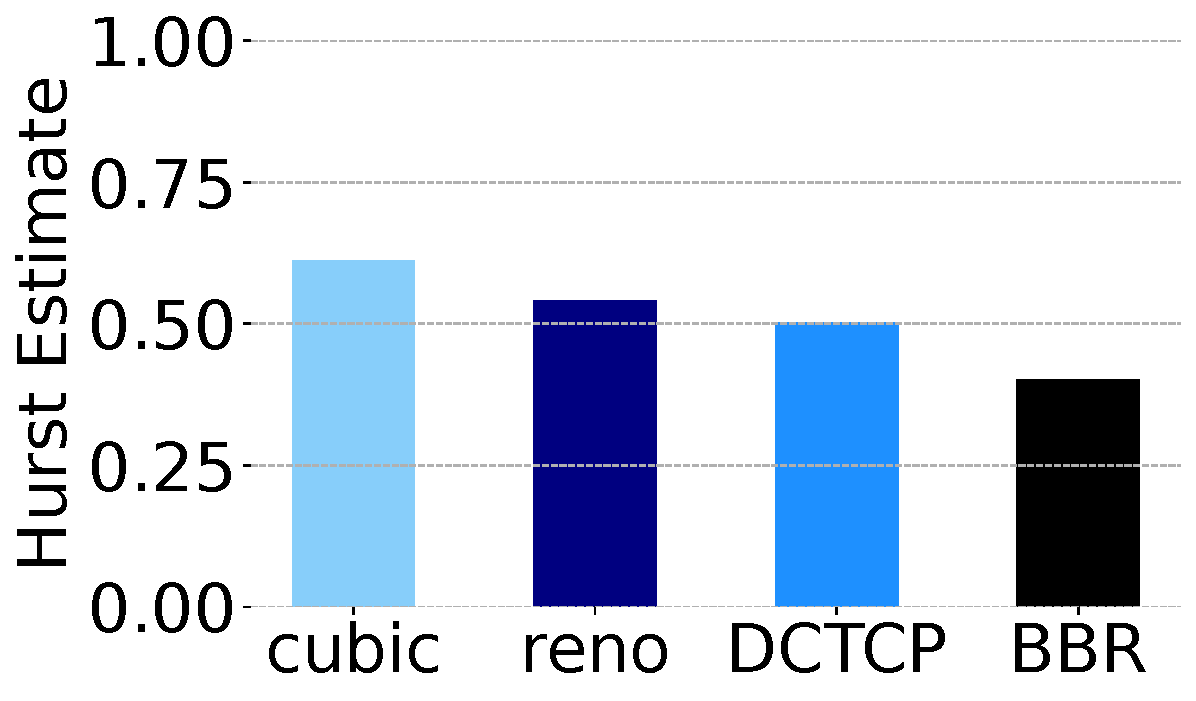
\includegraphics[width=1\linewidth]{figs/transport_hurst_bar.pdf}
    \caption{\small{H estimates for TCP variants suggest lower burstiness under BBR and DCTCP.}}
	\label{fig:transport-hurst}
     \vspace{-2mm}
\end{minipage}
\hspace{2pt}
\begin{minipage}[b]{0.45\textwidth}
    \centering
    	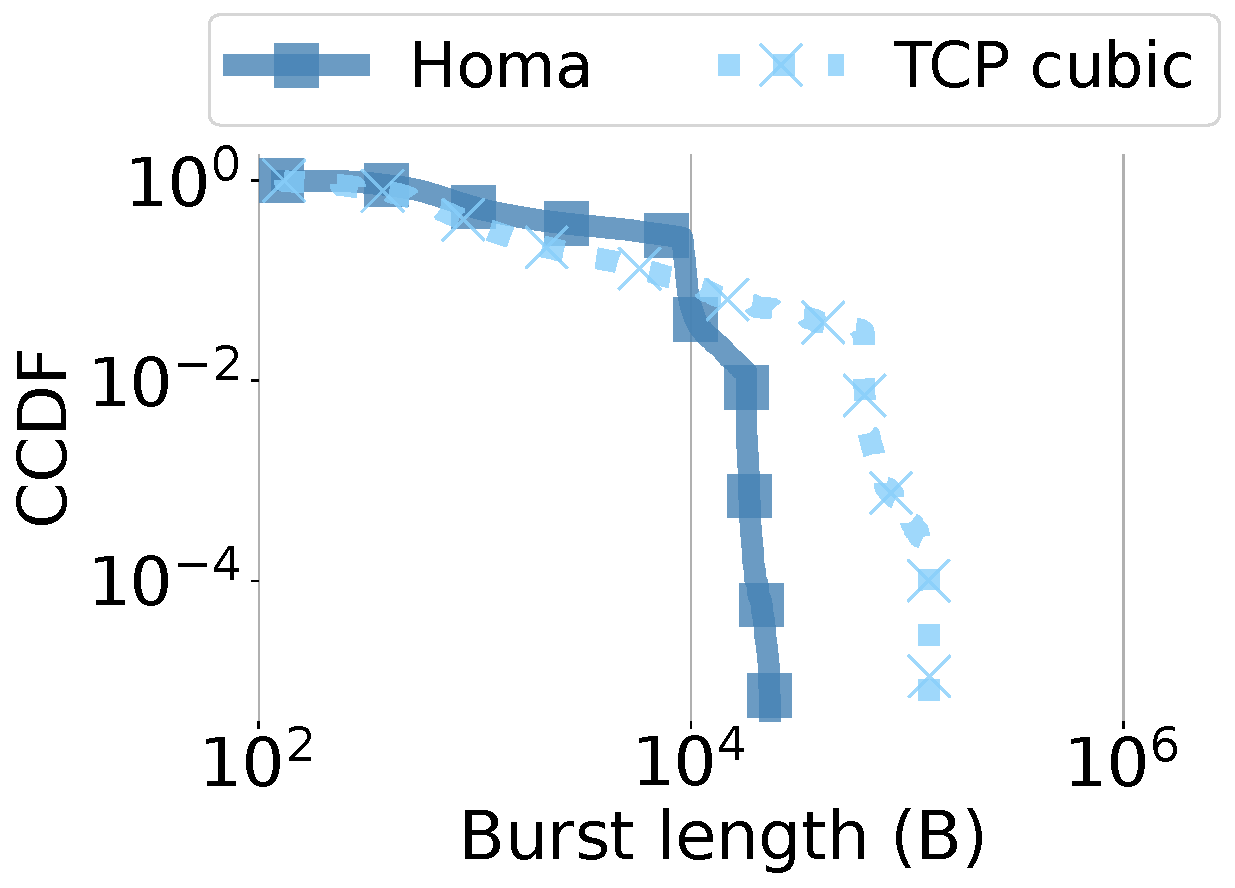
\includegraphics[width=1\linewidth]{figs/homa_ccdf.pdf}
    \caption{\small{A receiver-driven transport, Homa, is less bursty than TCP Cubic.}}
	\label{fig:transport-homa}
     \vspace{-2mm}
     \end{minipage}
\end{figure}



\subsection{Sources and implications of burstiness}
\label{sec:sources}
The previous section shows the aggregate impact of host networking elements on bursts. In this section, we measure the impact of each element, starting with the transport layer and moving to the elements that operate \emph{below} the TCP/IP stack (e.g., qdiscs) and \emph{in parallel} to it (e.g., the process scheduler).
%To find the culprits behind traffic burstiness, we direct our focus toward layers of network stack processing. Starting with the transport protocols, we investigate each layer separately by trying different configurations while keeping the rest of the systems fixed.




\subsubsection{Transports and congestion control}
Starting with transports, we evaluate four TCP congestion control variants under a mixture of background traffic and a small-scale incast traffic pattern where two sender machines target one receiver. The background traffic consists of two \textit{iperf} flows each taking 18Gbps of bottleneck link bandwidth. The incast traffic follows the map-reduce workload size distribution. For this experiment only, we run both the workload generators and the applications outside the container environment. Figure \ref{fig:transport-queue} shows how TCP Cubic \cite{cubic}, TCP Reno, DCTCP \cite{dctcp}, and BBR \cite{bbr} react to queue buildups in the network. 
Compared to Reno, TCP Cubic (the default congestion control setting in recent versions of Linux kernels) uses a more aggressive function for increasing its congestion window upon receiving acknowledgments. Therefore, it experiences larger queueing oscillations than Reno. BBR uses round-trip times to adjust its transmission window and varies its pacing rate to keep the in-flight bytes near its estimated bandwidth-delay product. Thus, it experiences a more steady queueing behavior while trying to keep the buffer half full. Finally, DCTCP uses explicit congestion notifications from switches to maintain consistently low queuing.

Figure \ref{fig:transport-ts} presents the throughput timeseries of the four congestion control variants at different timescales followed by their Hurst exponent estimates in Figure \ref{fig:transport-hurst}.
With the help of pacing and RTT estimations, BBR is able to maintain a steady throughput and a non-bursty traffic shape, reflected by $H = 0.40$.
On the other hand, Cubic's less conservative transmissions incur a self-similarity estimate of 0.60.

Finally, we deploy Homa's kernel module \cite{homa} as a representative implementation of receiver-driven transports in the Linux kernel. In receiver-driven transports, the destination initiates more packets by issuing \textit{grant} control packets for the sending host. In our setup, Homa sends the first 90 KB of each flow unscheduled as an attempt to initiate the communication and retrieve the path's congestion status. The following packets are then scheduled using grants. 
Due to its limited implementation scope, the Homa module is not able to achieve line rate performance. Therefore, we limit our observation to the map-reduce workload tuned down to 6 Gbps offered load. 
Figure \ref{fig:transport-homa} presents the burst lengths for Homa and TCP Cubic as observed by Valinor-H eBPF framework. We observe that the p99 burst length under Homa is 9$\times$ lower than Cubic which might reflect two facts. First, unlike Cubic which sends up to 64 KB long data chunks, Homa's prepared \textit{sk\_buff} chunks are mostly as large as its MTU (9 KB in this experiment). This is also due to the fact that Homa kernel module is not making use of TSO because of certain Intel NIC limitations. Secondly, Homa uses pacing to keep the NIC fully saturated in its Linux implementation which further controls the spacing between its transmissions \cite{homa-impl}.
%
Combined, these factors result in Homa's less bursty behavior compared to TCP Cubic, not just at small timescales (Figure \ref{fig:transport-homa}) but also at large timescales ($H=0.54$ for Homa \emph{vs.} 0.62 for Cubic). However, we suspect a different behavior from Homa on different setups that can make use of NIC offloading.



\subsubsection{Software switching}
\label{sec:qdisc}
Linux leverages queueing disciplines (\textit{qdiscs}) to enforce scheduling among segments originating from different applications in the system. If generic segmentation offload is not in use, \textit{qdiscs} are the last software components to decide the order of data entities on NIC's FIFO rings.
We study five representative queueing disciplines implemented in Linux:
\\
\textbf{1) Fair queue (fq)} is the default scheduler in recent Linux kernels and is mainly used to enforce pacing on a per-flow (per socket) basis. The appropriate pace among flows is either explicitly enforced via socket options, or is determined by the TCP congestion control (e.g., BBR). By default, \textit{fq} uses deficit round-robin with a default quantum of 3028 bytes to drain flow queues, with an initial quantum equalling TCP's initial 10-packet window.
% \\
% \textbf{2) CHOKe (CHOose and Keep for responsive flows, CHOose and Kill for unresponsive flows)} is an Active Queue Management (AQM) algorithm aimed at preventing bufferbloat \cite{bufferbloat}. CHOKe is a variant of the Random Early Drop (RED) scheme and uses a randomized algorithm to enforce early drops on flows that monopolize the queue.
\\
\textbf{2) fq\_CoDel.} The controlled delay (CoDel) algorithm, combined with fair queue, enforces CoDel on per-flow sub-queues. CoDel, a more recent AQM algorithm, uses packet sojourn time inside each flow queue to detect slow flows and prevents the queueing delay to exceed a user-specified target by dropping excess traffic.
\\
\textbf{3) Stochastic Fair Queueing (SFQ)} extends flow-queuing with random-early marking/drop semantics with small default queue sizing to control the queueing delay. Similar to \textit{fq}, it uses round-robin scheduling on per-flow sub-queues. SFQ uses a default deficit of one MTU.
\\
\textbf{4) pfifo\_fast} is a First-In First-Out priority queue. Higher priority packets are distinguished by their Type of Service (TOS) fields in IP headers which are set by upper layers.
\\
\textbf{5) Heavy Hitter Filter (HHF)} attempts to identify and separate short flows from heavy hitters to prevent head-of-the-line blocking and increased delays for latency-sensitive flows. Such flows are given a higher deficit compared to heavy hitters in each transmission round.

We study qdiscs under three scenarios: First, to see the actual contribution of qdiscs to the traffic shape, we disable segmentation offload and serialization offload and limit the number of the transmit rings to one (single-queue). Segmentation is the process of breaking large \textit{sk\_buffs} into MTU-sized segments and is usually deferred to the last processing stages to reduce CPU utilization and improve flow performance. Segmentation offload can either be performed in the hardware (TCP Segmentation Offload or TSO) or just before passing the data to the hardware (Generic Segmentation Offload or GSO). Additionally, in a multi-queue architecture, the network stack communicates to the NIC via separate ring buffers pinned to each CPU core to reduce inter-core communication overheads and improve throughput. When enabled, a (reportedly, round-robin \cite{titan}) packet scheduler in the hardware will decide the order in which packets are drained from ring buffers.

Initially, we run 1000 Iperf instances spread across 200 containers, simulating the map-reduce workload on the single-queue server without offloading. Figure \ref{fig:qdisc} demonstrates how, \emph{in isolation}, per-flow queuing can significantly shorten the size of egress bursts. Techniques such \textit{pfifo\_fast}, and HHF use one large buffer containing packets from all egress flows, allowing multiple data segments of one flow to be enqueued simultaneously. On the other hand, per-flow queueing allows the scheduler to interleave among packets of different flows, primarily to maintain fairness and prevent head-of-the-line blocking \cite{backdraft}.

To verify the impact of round-robin scheduling on blunting bursts, we repeat the same experiment with \textit{fq} qdisc, increasing the per-flow deficit from one MTU (1514 bytes) to 16 MTUs, and observe a linear correlation between fq deficits and burst lengths. For example, the 90$^{th}$ percentile of burst lengths under a deficit of 16 packets is increased to 25 KB from 13 KB under that of 8 MTUs (92\% increase). 
% This also explains why SFQ qdiscs is the least bursty in the previous experiment.

\begin{figure*}[t]
\centering
\begin{subfigure}[t]{0.32\linewidth}
    \centering
    	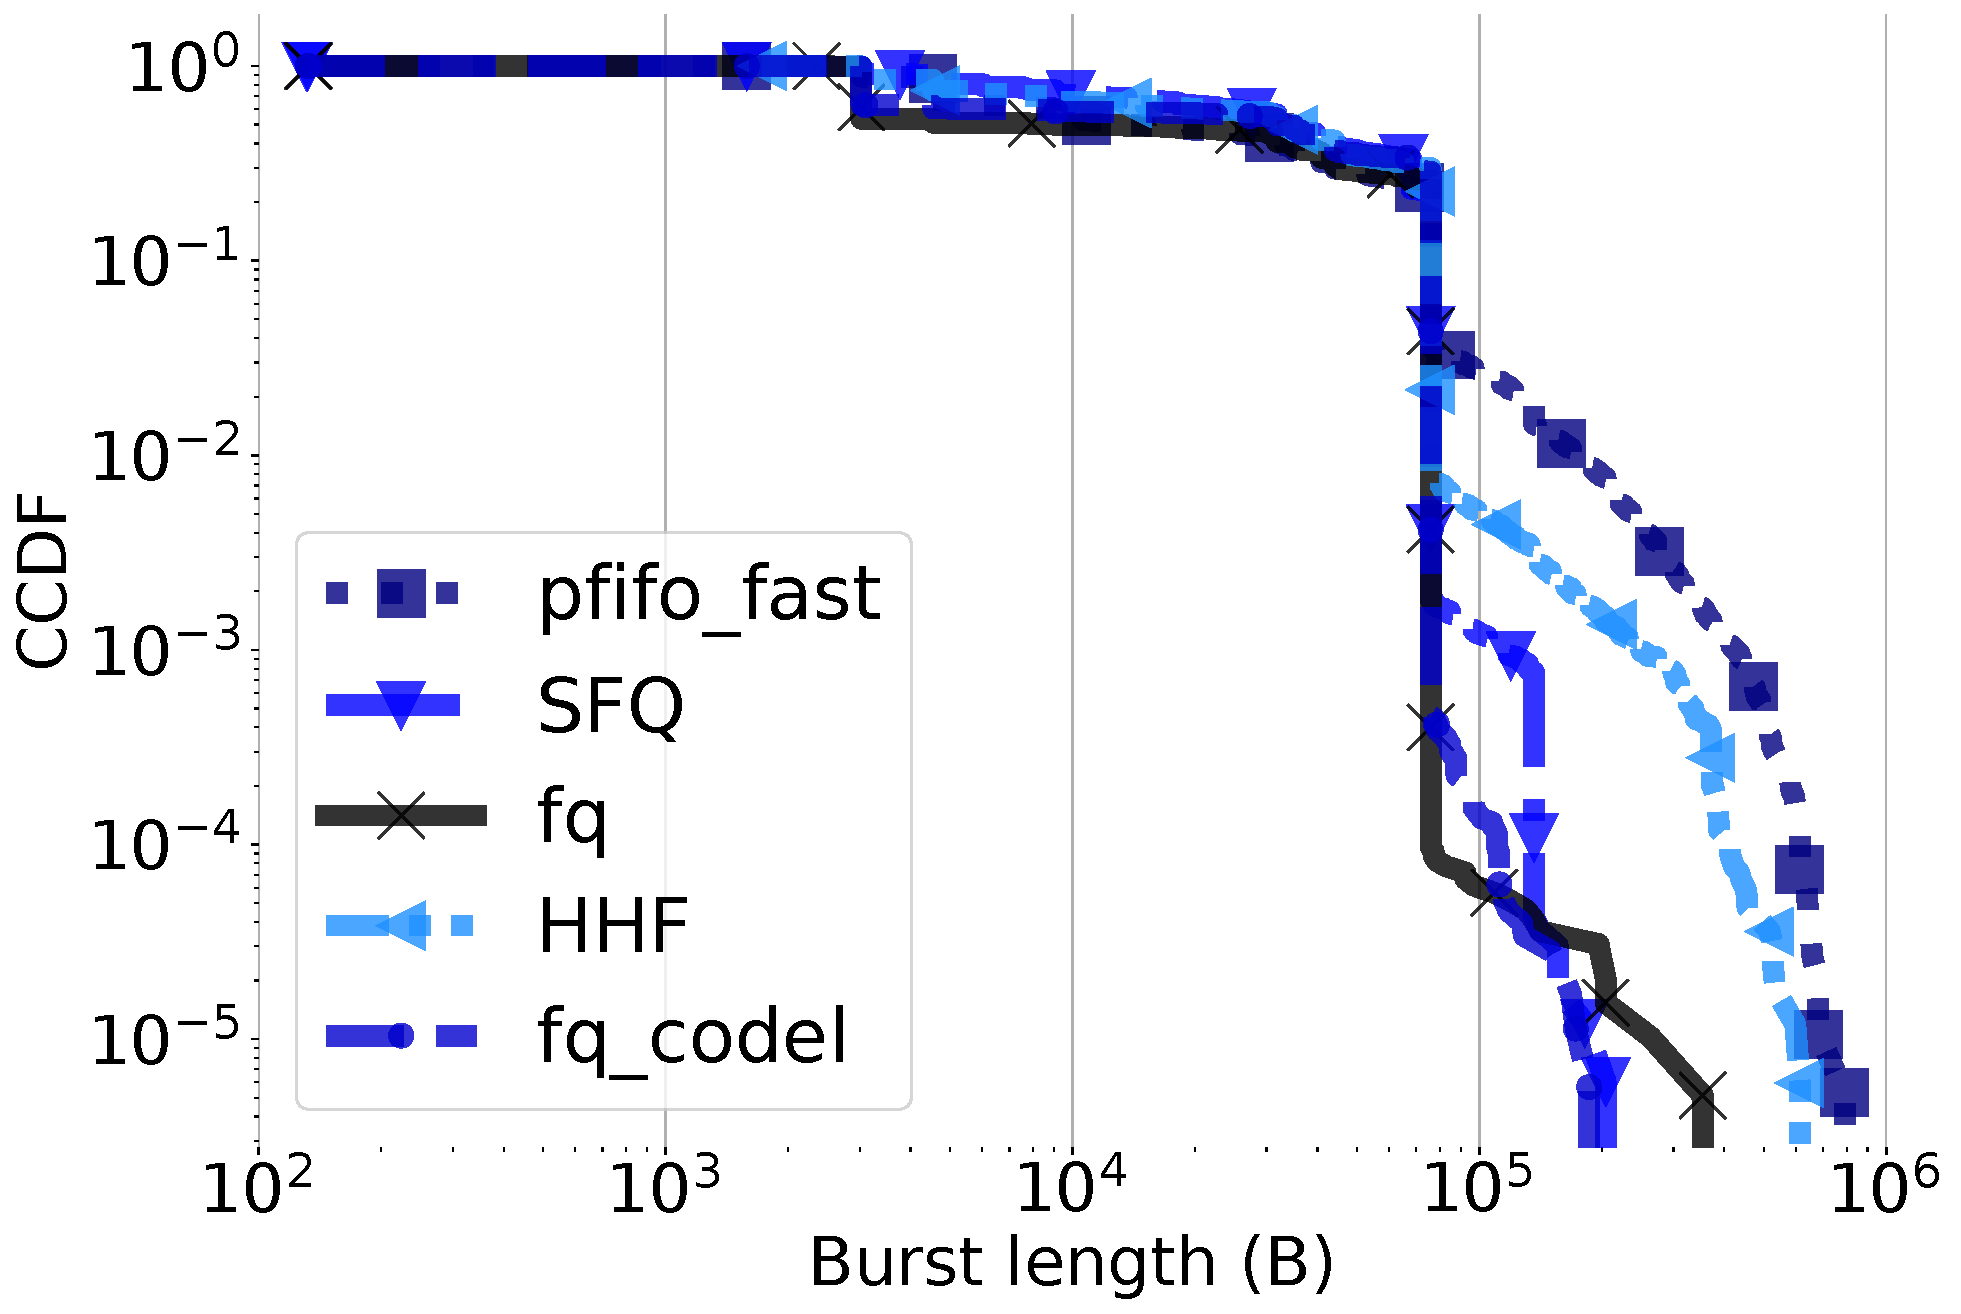
\includegraphics[width=1\linewidth]{figs/26_4.pdf}
    \caption{SQ w/out Offloading}
	\label{fig:qdisc}
\end{subfigure}
\begin{subfigure}[t]{0.32\linewidth}
    \centering
    	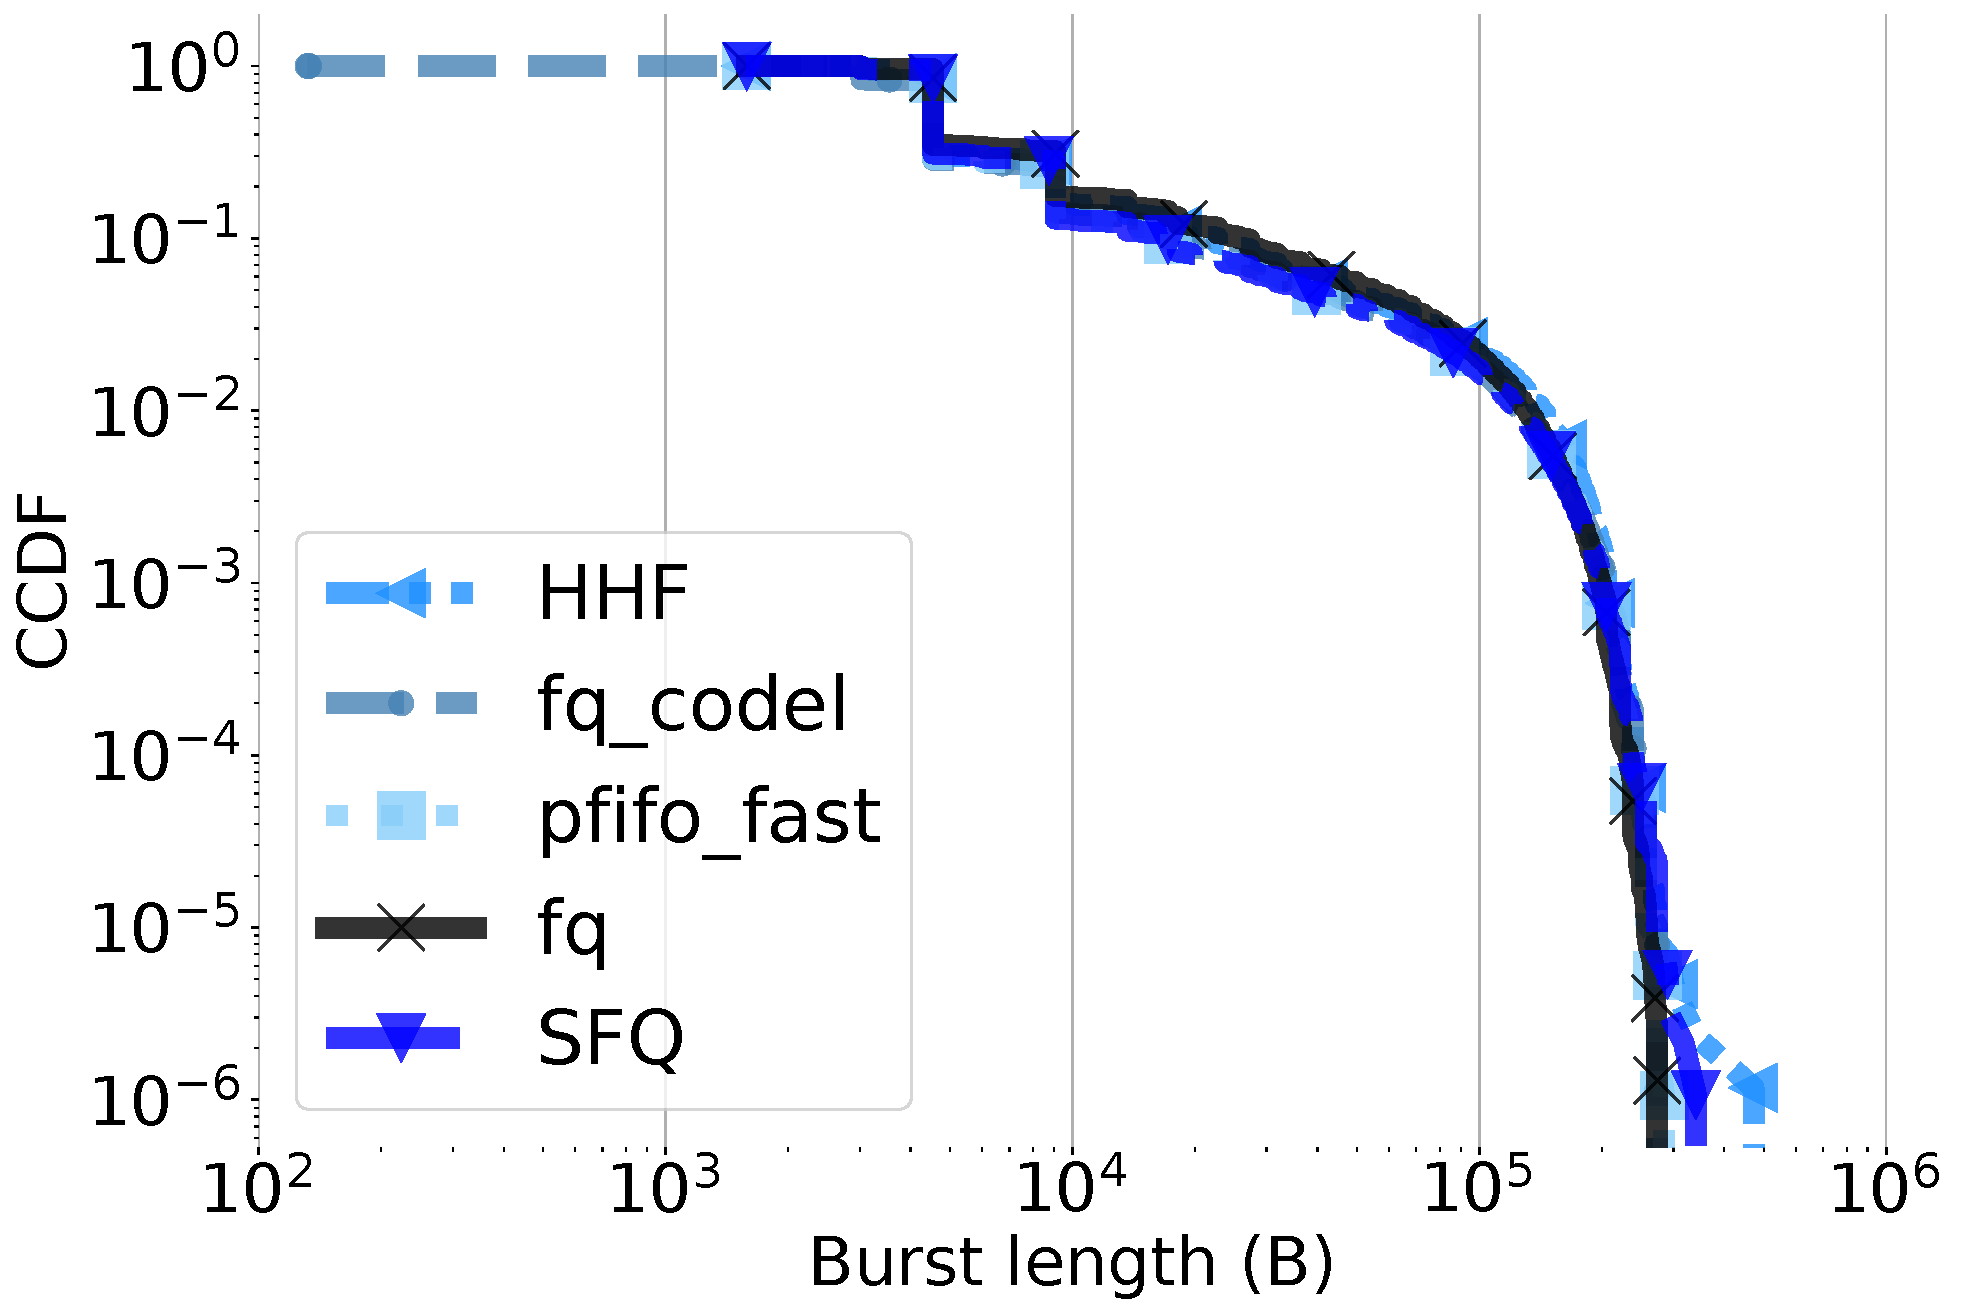
\includegraphics[width=1\linewidth]{figs/26_6_fig.pdf}
    \caption{SQ w/ Offloading}
	\label{fig:qdisc_tso}
\end{subfigure}
\begin{subfigure}[t]{0.32\linewidth}
    \centering
    	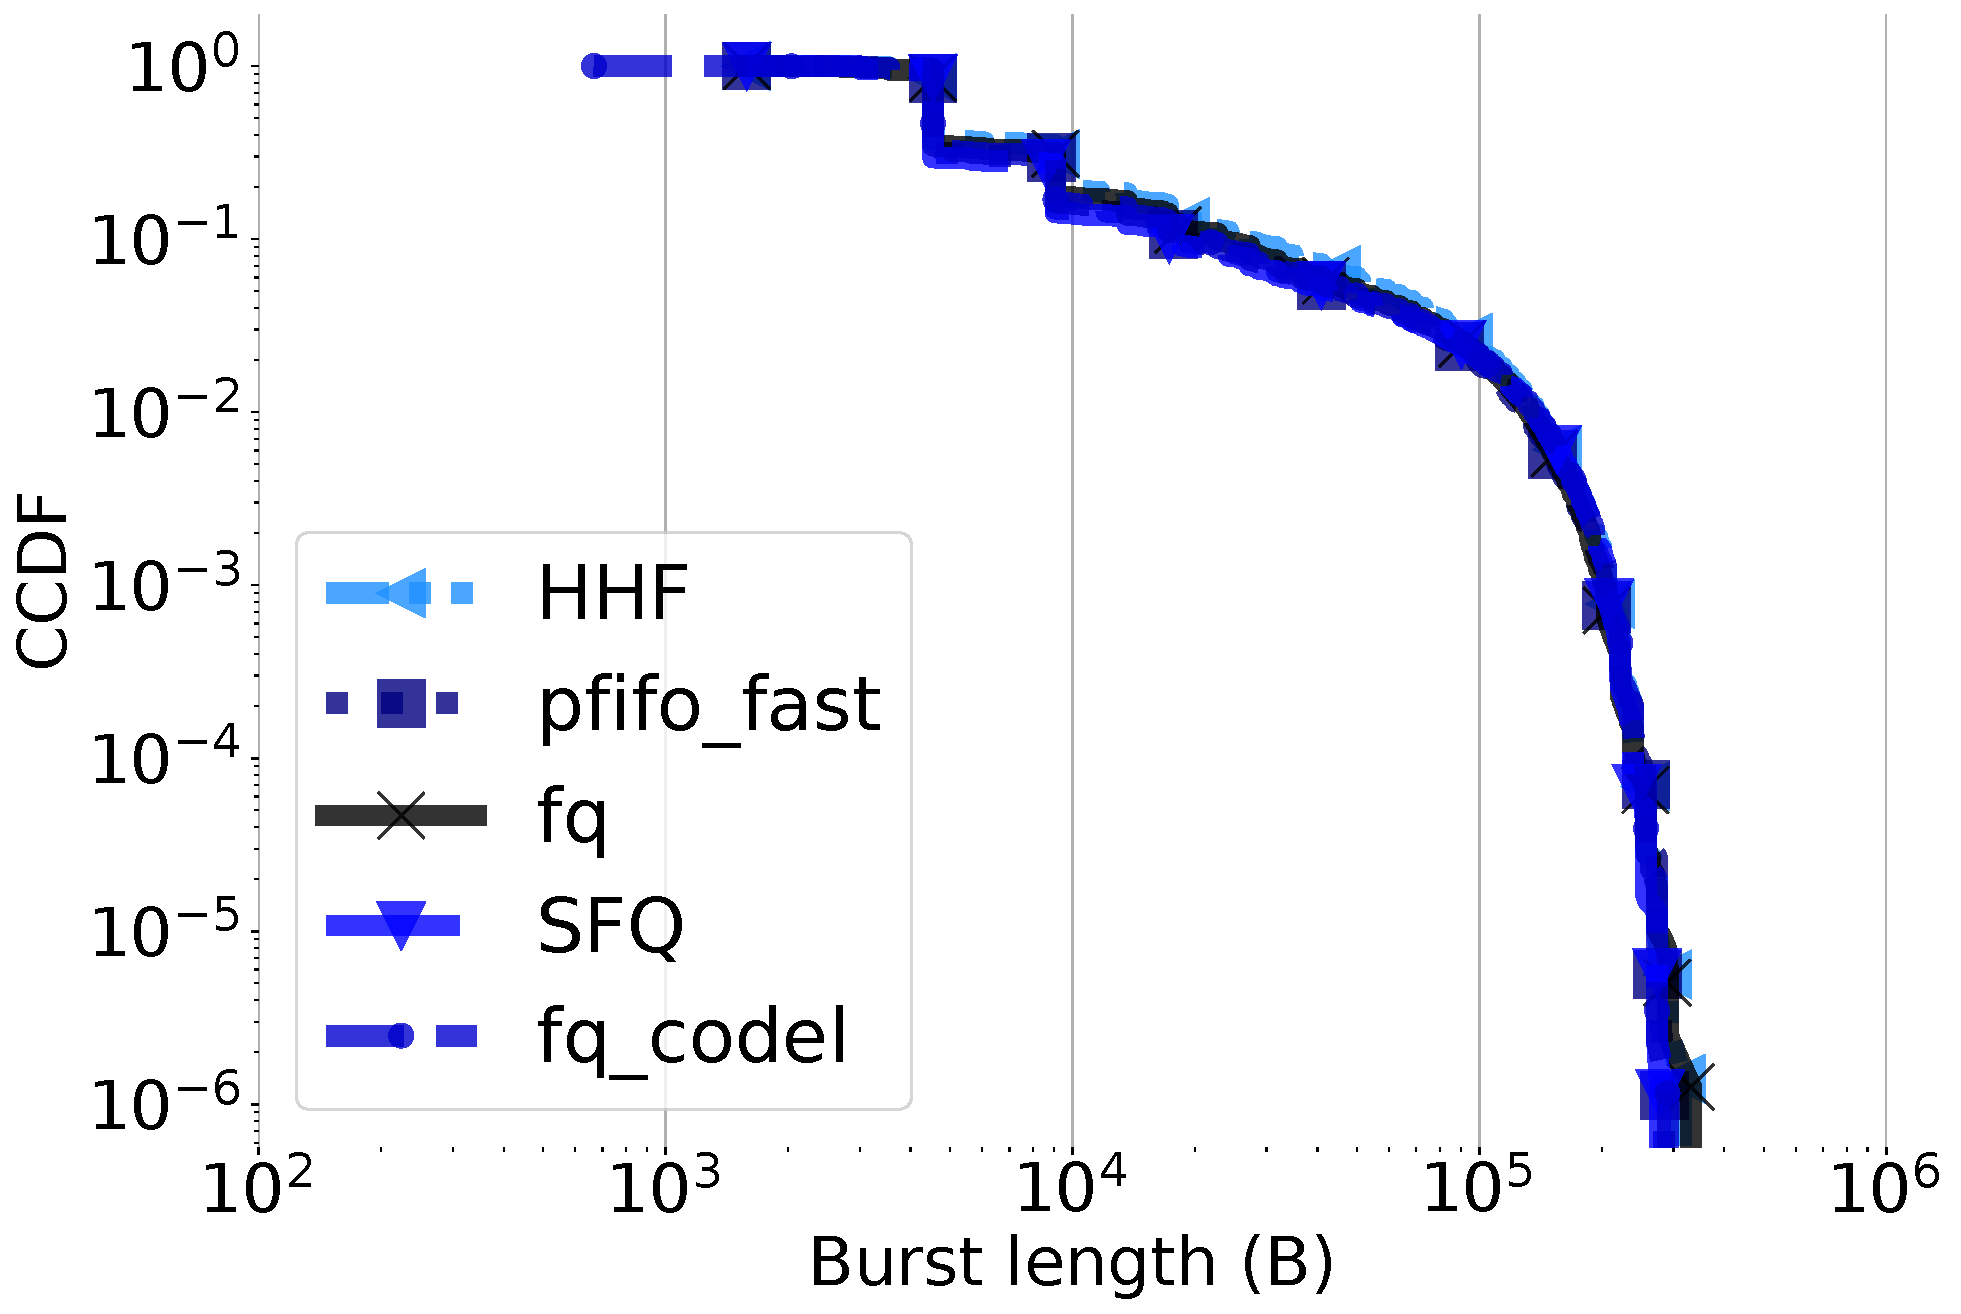
\includegraphics[width=1\linewidth]{figs/26_2.pdf}
    % 	\vspace{5mm}
    \caption{MQ w/ Offloading}
	\label{fig:qdisc_mq}
\end{subfigure}

\vspace{-2mm}
\caption{\small{Both Multi-queueing (MQ) and TCP segmentation offload compromise the intended shape of software packet scheduling.}}
\vspace{-2mm}
\end{figure*}

While qdisc is the last layer to perform packet scheduling in the software, the traffic ultimately often passes through segmentation offloading and NIC scheduling before reaching the wire. Is the impact of qdiscs on the wire preserved \emph{after the interaction} with these lower layers?
To investigate, we enable all the offloading features and perform our measurements again. Figure \ref{fig:qdisc_tso} demonstrates the impact of offloading segmentation and serialization on lengthening the egress bursts. SQ represents Single Queue NICs while MQ represents Multi-queueing combined with a layer of round-robin scheduling at the NIC. With TSO at work, qdiscs no longer serve packets. Instead, they schedule between dynamically sized \textit{sk\_buffs}. Hardware offloading then helps increase the throughput by nearly 50\% for all cases while moving the buffering to the hardware where large segments are broken into MTU-sized packets and sent on the wire. This significantly undermines qdisc's decisions on shaping the traffic. With offloading in action, the median burst sizes for \textit{fq}, \textit{fq\_codel}, and \textit{pfifo\_fast} are, 132 kB, 127 kB, and 127 kB, respectively. While without offloading, these systems experienced a median burst length of 76 kB, 76 kB, and 172 kB\footnote{pfifo\_fast combined with offloading can exacerbate burstiness as both layers are prone to creating large, uncontrolled bursts.}, respectively.

\begin{figure}[t]
\centering
\begin{subfigure}[t]{0.75\linewidth}
    \centering
    	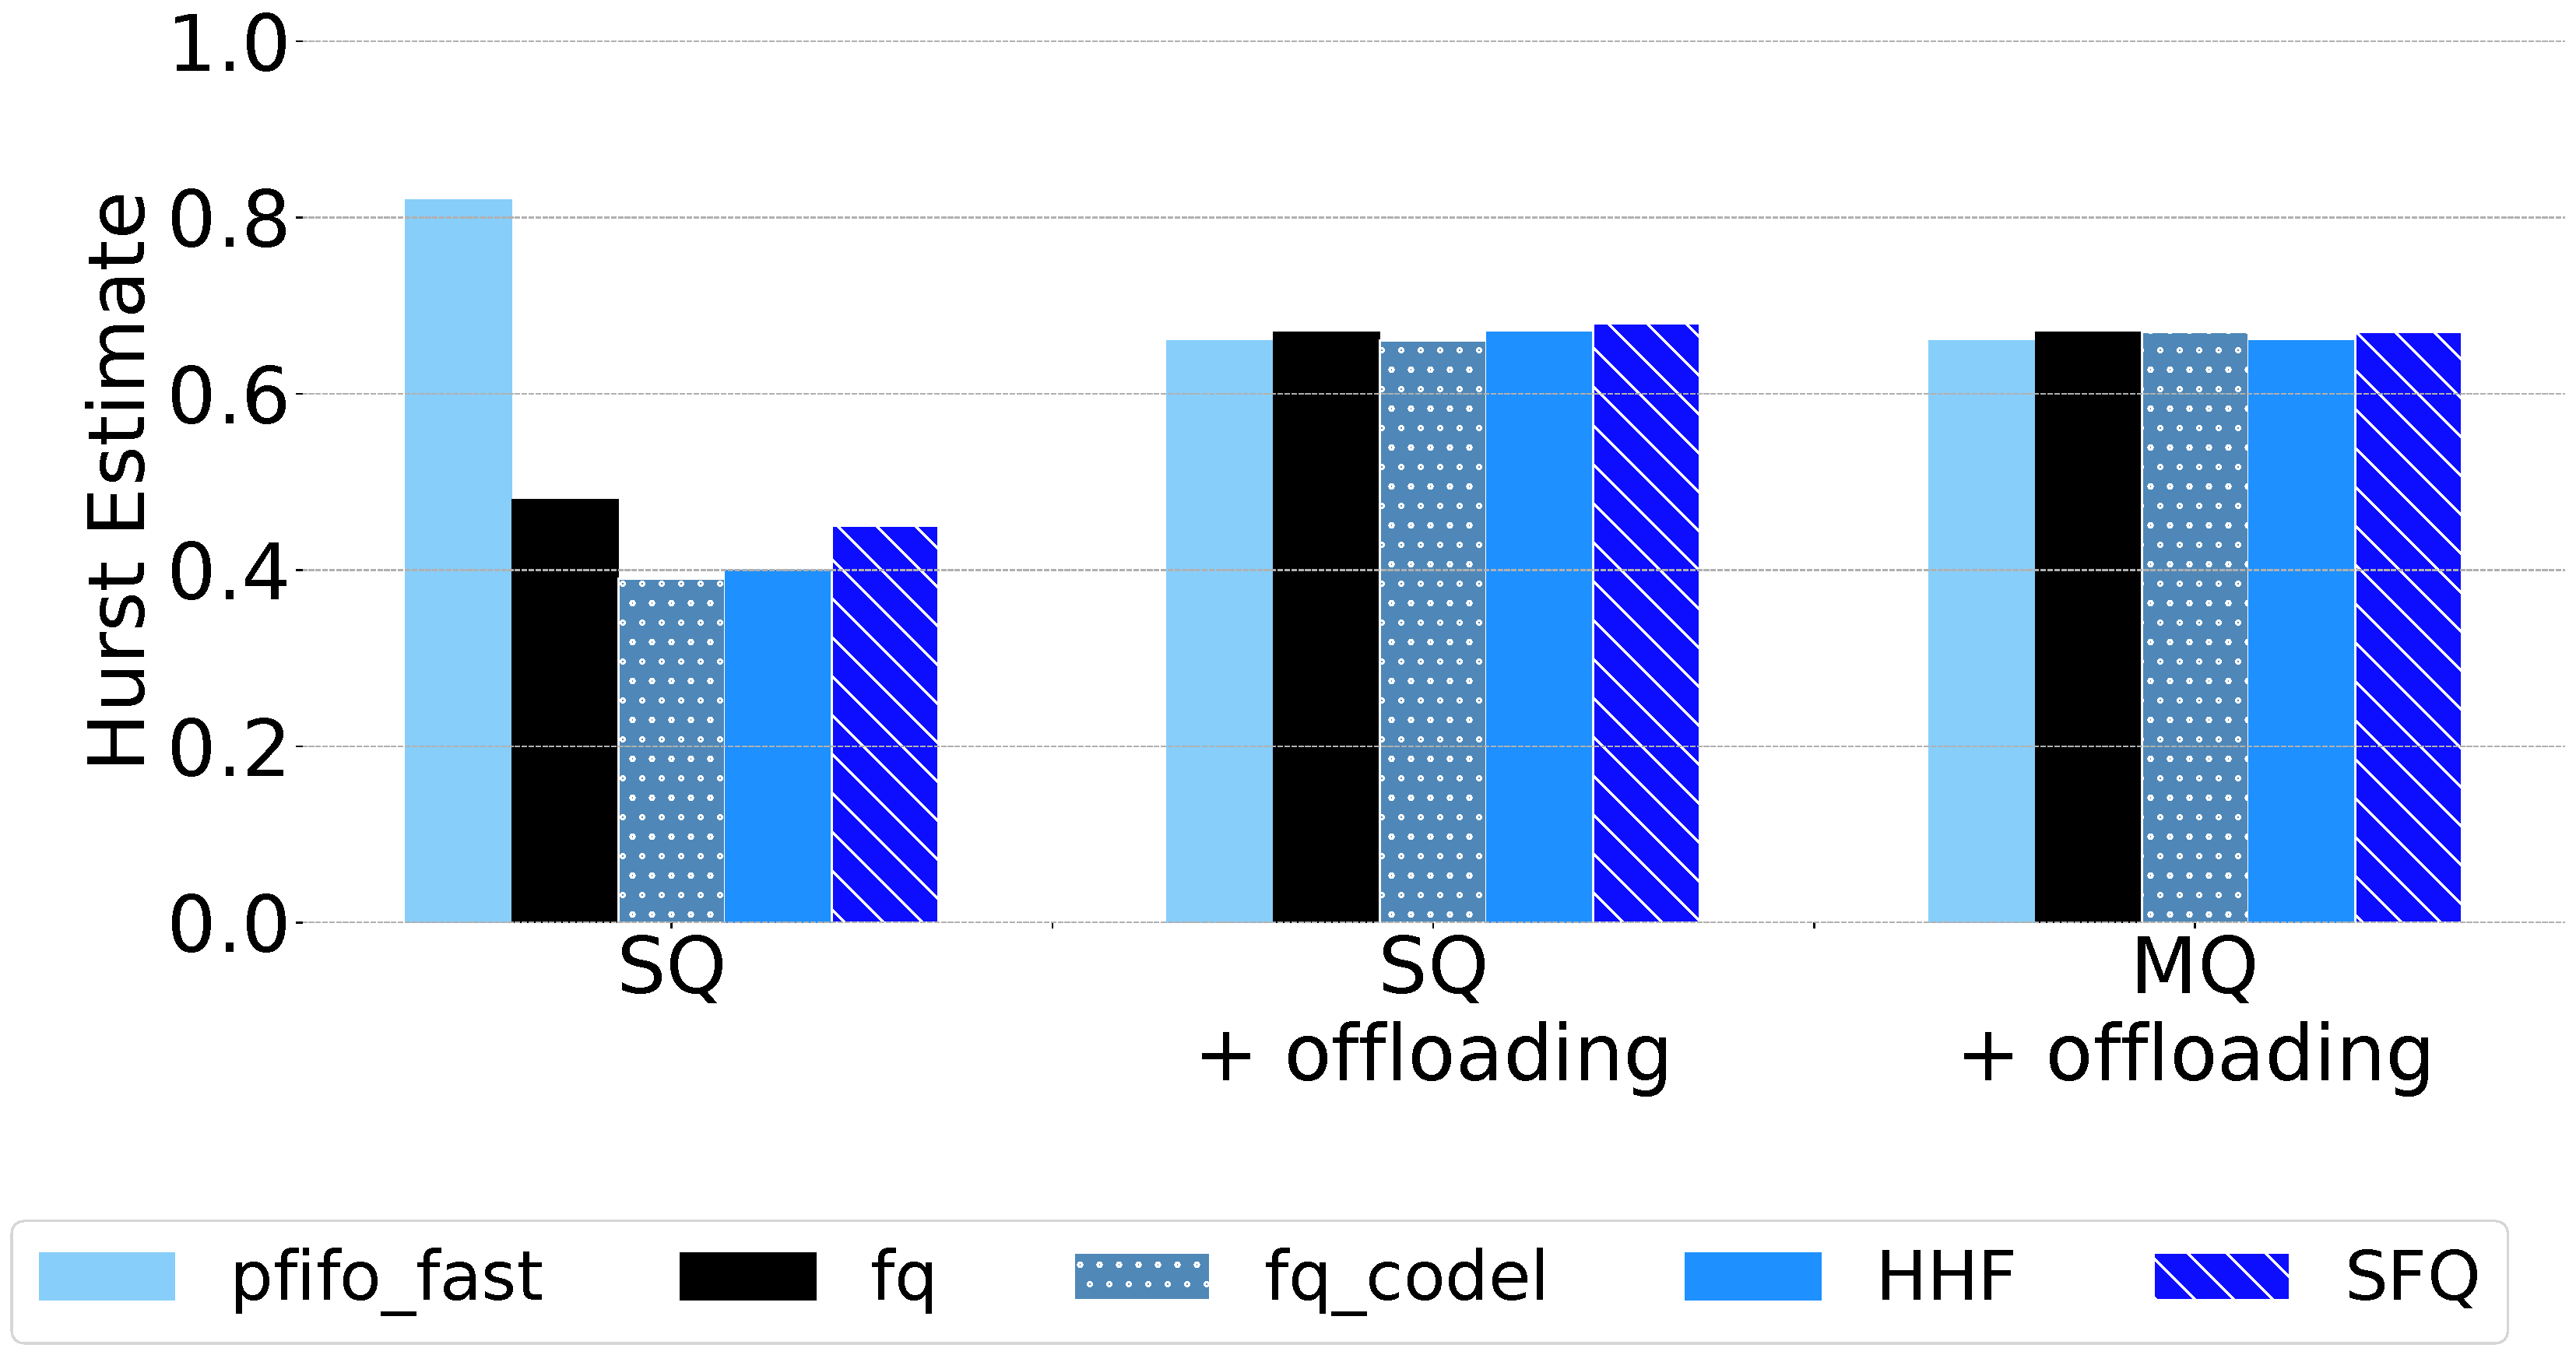
\includegraphics[width=1\linewidth]{figs/nic_hurst_bar.pdf}
    % 	\vspace{5mm}
    % \caption{\small{\textbf{Hurst estimates}}}
\end{subfigure}
\vspace{-2mm}
\caption{\small{Hurst estimates for different Linux packet schedulers.}}
	\label{fig:nic_hurst_bar}
\vspace{-2mm}
\end{figure}

To further ruffle the output of qdiscs, we enable the default multi-ring root qdisc which assigns a separate qdisc instance to each CPU core and enables the NIC scheduler to perform last-level scheduling on transmit rings (multi-queue architecture). Figure \ref{fig:qdisc_mq} presents the outcome. \textit{With NIC scheduling and segmentation offloading at work, the shape of the qdisc's outgoing traffic is barely preserved on the wire.} That is because, NICs are equipped with internal round-robin schedulers to drain the software rings, further reducing the chances of creating long bursts. Finally, Figure \ref{fig:nic_hurst_bar} demonstrates the estimated Hurst exponents for the three scenarios. Without segmentation offloading, the degree of burstiness is considerably reduced (H < 0.5) for all but one case. Only \textit{pfifo\_fast} which does not offer any form of fair queueing suffers from heavier burstiness ($H=0.8$) under the single-queue scenario.
\\
\textbf{Implications of disabling offloading and multi-ring scheduling.}
Apart from burstiness, both offloading and NIC scheduling have a profound impact on flow performance metrics. Our measurements demonstrate that disabling TCP segmentation offload for a workload consisting of 1000 same-size flows results in 71\% decline in median flow throughput, 46\% increase in median packet RTTs, and 3$\times$ increase in sender CPU utilization. Therefore, disabling offloading, in order to enable software control is not always a viable option. 
Multi-queue NICs are also considered a quick solution with potential side effects. While enabling multi-queue reduces resource contention, they can increase response times and are usually fixed-function \cite{titan}.

% \begin{tcolorbox}

% \textbf{Finding x}
% Single-queue disciplines demonstrate uncontrolled burstiness in the absence of NIC scheduling and offloading. With offloading and multi-ring scheduling enabled, qdiscs can barely impact the shape of egress traffic.
% \end{tcolorbox}

% \begin{tcolorbox}

% \textbf{Finding x}
% Scheduling disciplines that use deficit round-robin with a large quantum are prone to producing longer $\mu$bursts.
% \end{tcolorbox}

\begin{figure}
    \centering
    \begin{subfigure}[t]{0.40\linewidth}
    \centering
    	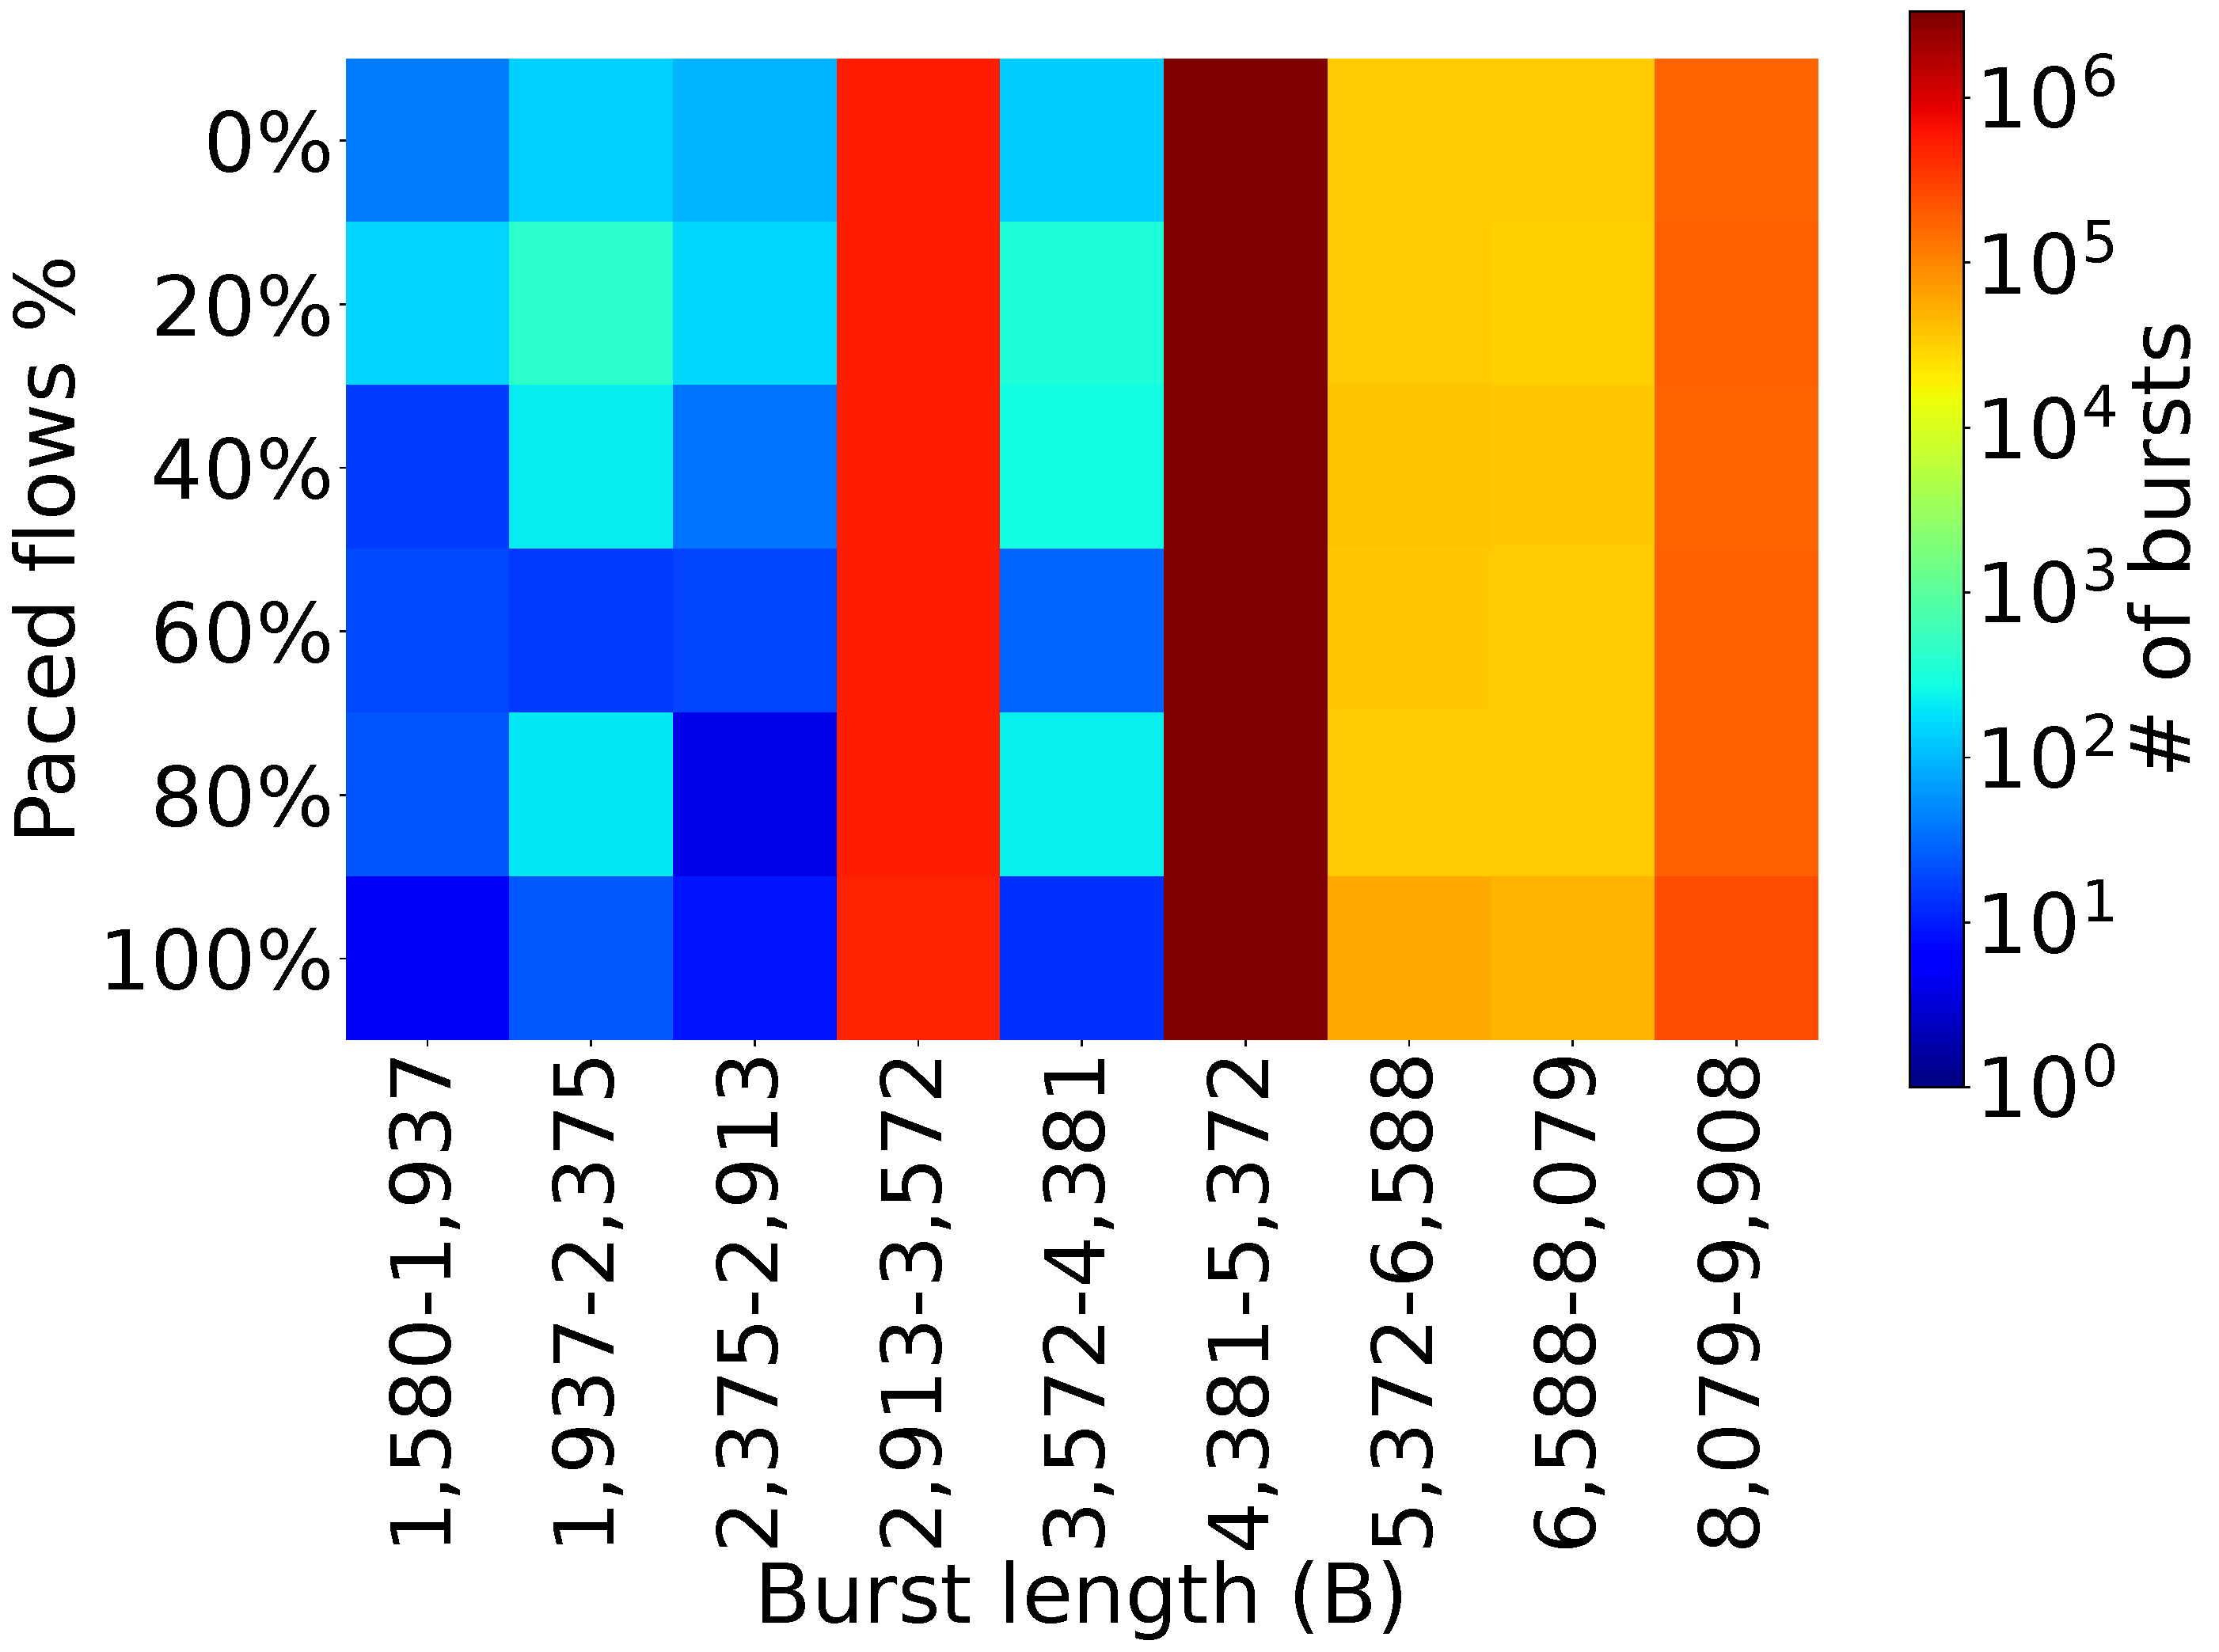
\includegraphics[width=1\linewidth]{figs/pacing1.pdf}
    	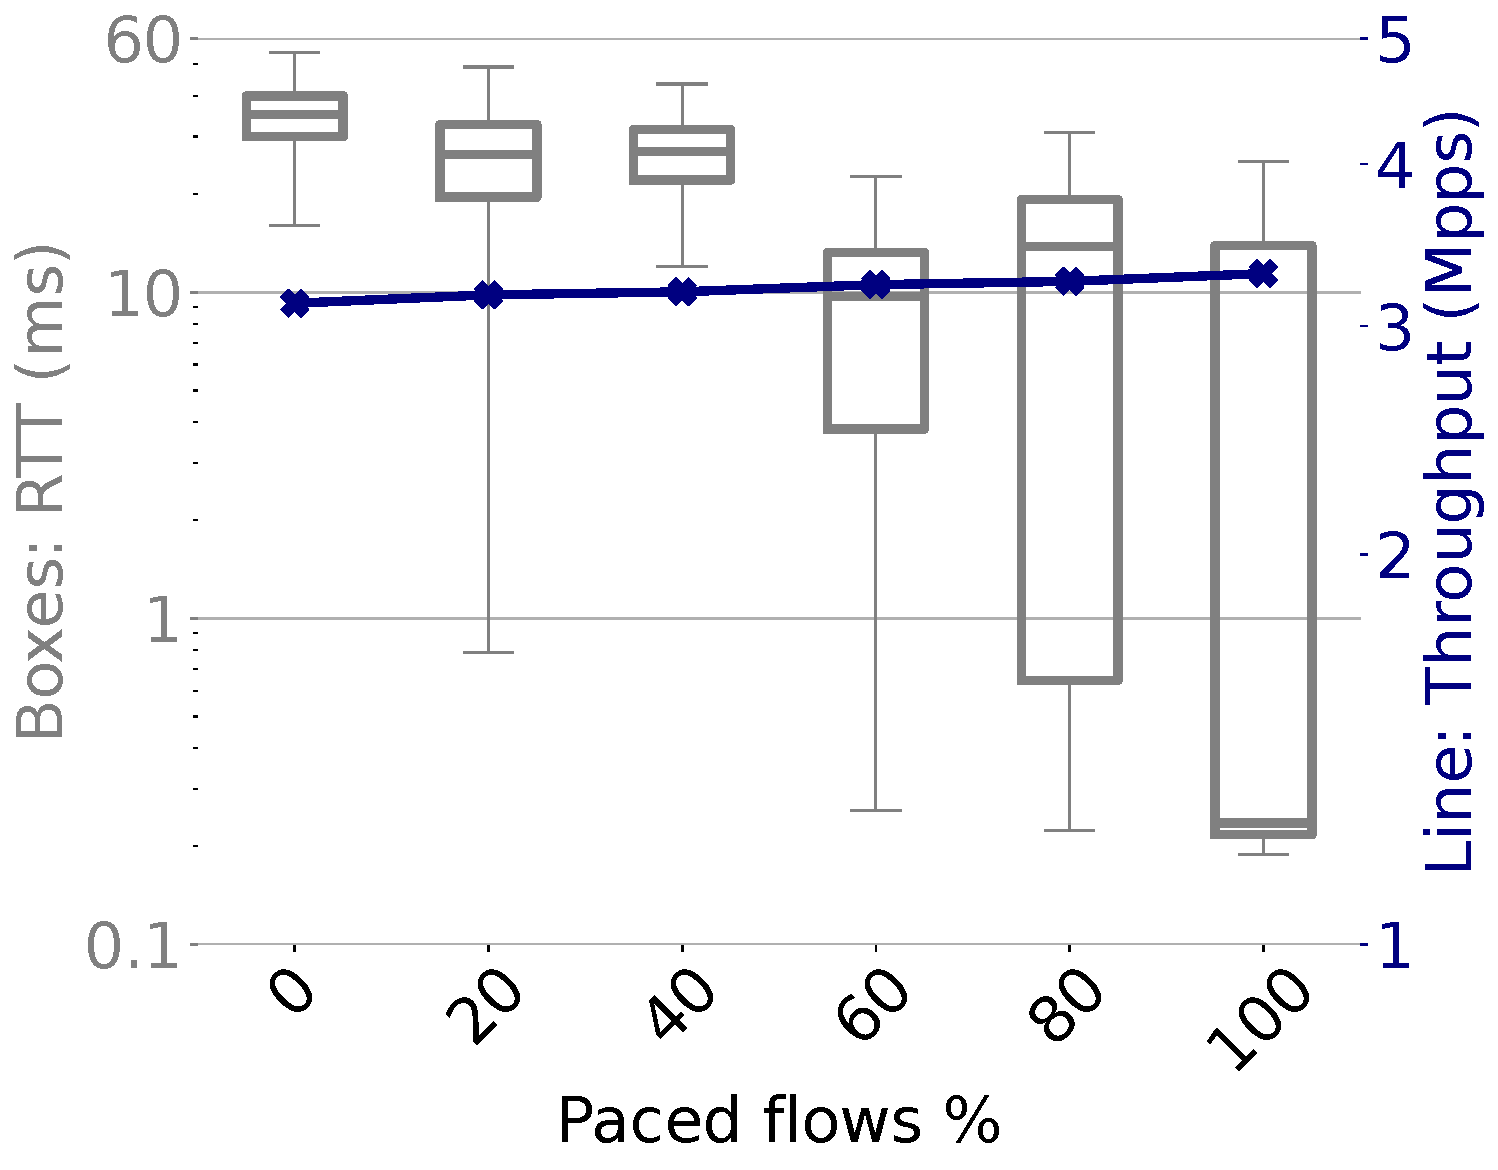
\includegraphics[width=1\linewidth]{figs/pacing_intra_rack_rtt_tput.pdf}
    \caption{Intra-Rack M/R}
	\label{fig:pacing_rack}
\end{subfigure}
\begin{subfigure}[t]{0.40\linewidth}
    \centering
    	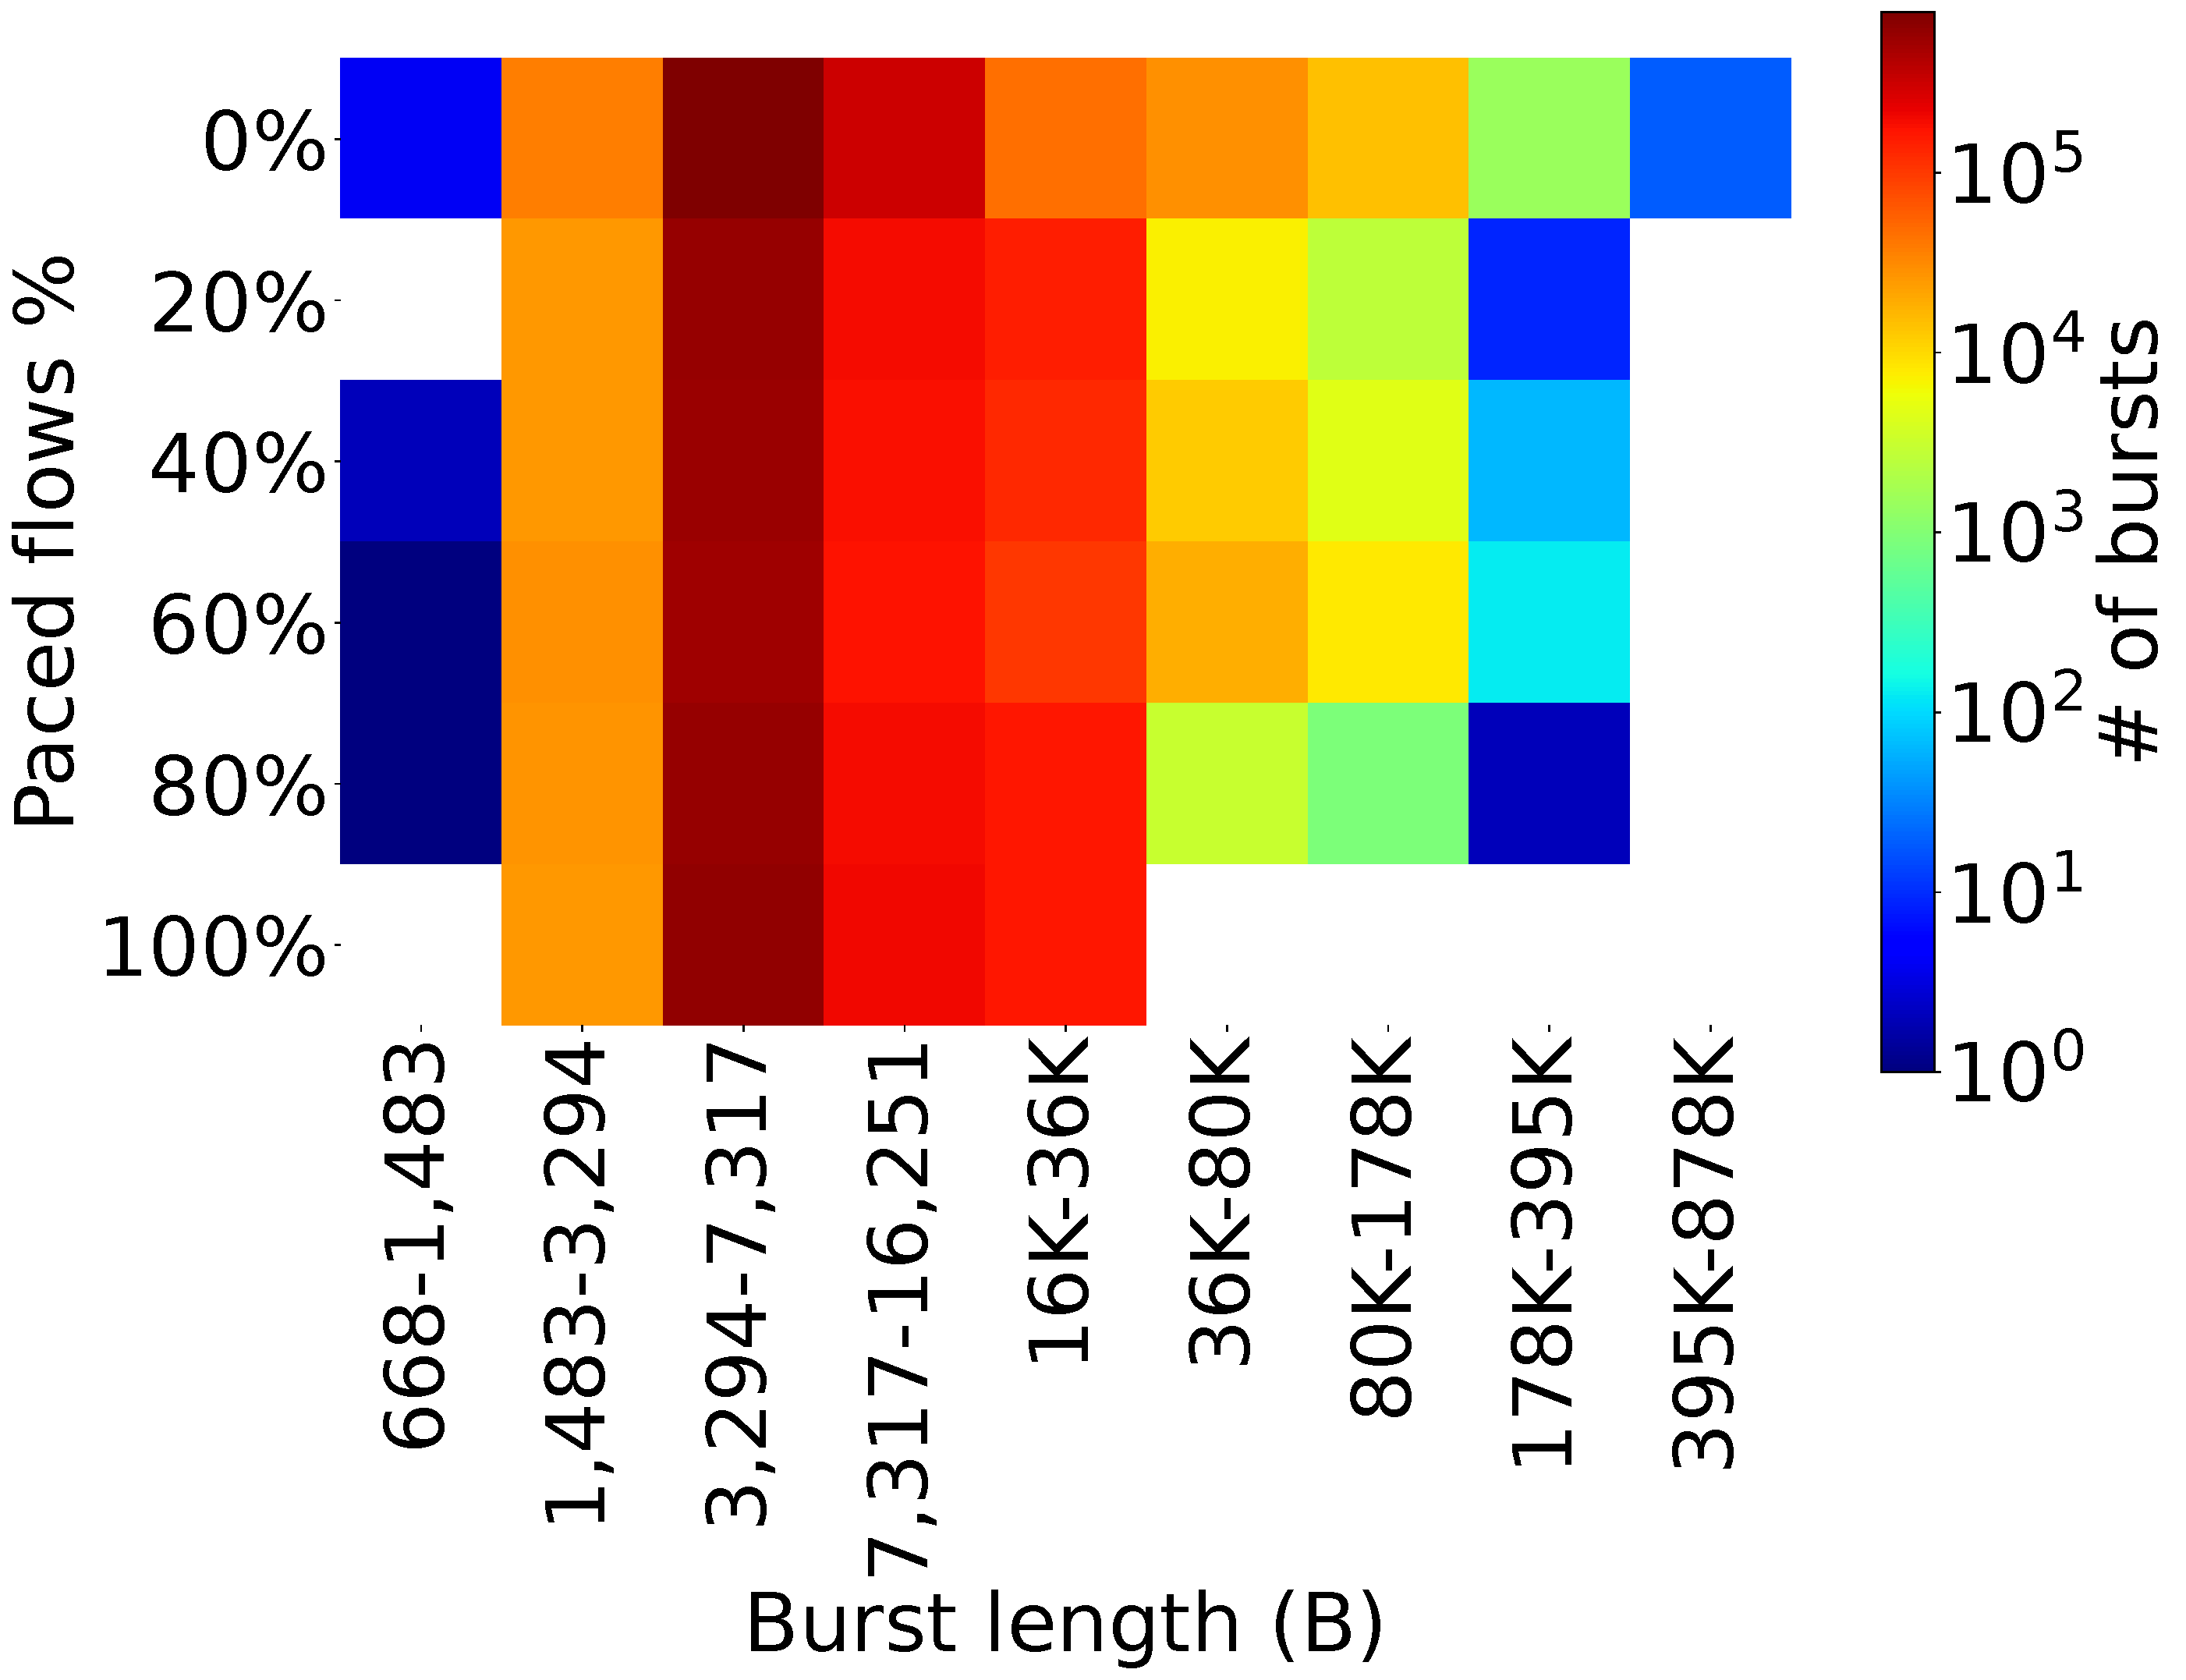
\includegraphics[width=1\linewidth]{figs/pacing2.pdf}
    	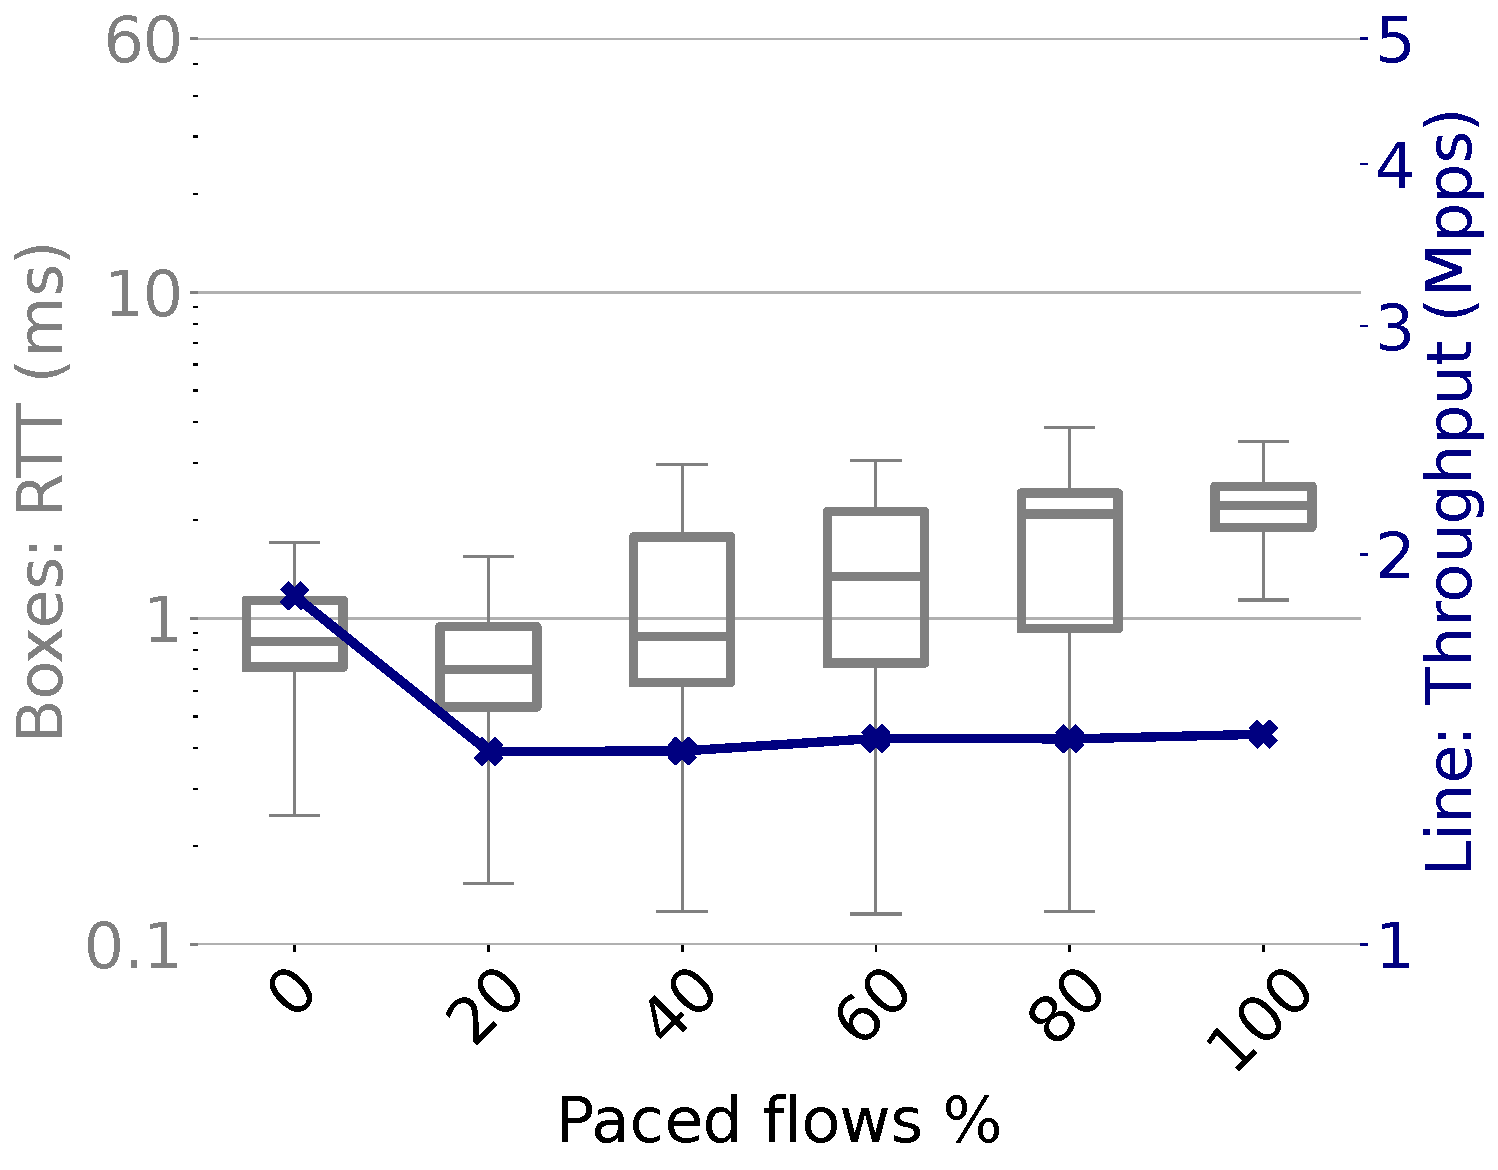
\includegraphics[width=1\linewidth]{figs/pacing_intra_cluster_rtt_tput.pdf}
    \caption{Intra-cluster M/R}
	\label{fig:pacing_cluster}
\end{subfigure}
    	% \vspace{-2mm}
    \caption{\small{Software pacing is workload dependent. For workloads consisting of large flows, its impact on smoothing bursts is unmade by lower layers. For workloads with both short and long flows, it reduces throughput.}}
    \vspace{-2mm}
	\label{fig:pacing}
\end{figure}

\subsubsection{Software pacing}
\label{sec:pacing}
The above observations raise another important question on host networking design decisions. While many congestion control techniques \cite{bbr,homa,swift,outcast,pacing} advocate for pacing in order to achieve accurate control over in-transit data, existing pacing implementation in the Linux kernel is deeply away from the wire, at fq qdisc. \emph{Are qdiscs a suitable place for enforcing pacing?}
To investigate, we repeat the map-reduce (M/R) workloads on the server with both offloading and NIC scheduling enabled and observe that \textit{for workloads with large flows (intra-rack M/R), pacing doesn't have a significant impact on burstiness, and for those with short flows (intra-cluster M/R), pacing results in throughput reduction.} Overall, our results highlight the limitations of software pacing for data center workloads.



Concretely, we configure \textit{fq} to pace 200 flows based on their fair share of bandwidth (200 Mbps), and gradually increase the portion of the flows that are counted as heavy hitters from 0\% (no flow is paced) up to 100\% (all flows are paced).
Figure \ref{fig:pacing} compares the bursts for (a) workload with mostly large flows and (b) workload with a mix of small and large flows. 
In the former workload, we observe that while the impact of pacing ratio is less evident, pacing allows for better bandwidth allocation and the line rate is preserved for all rows. On the other hand, in the latter workload, the throughput is reduced by 22\% under pacing.
This is because short flows are not able to make up for the freed bandwidth that pacing creates.
We also compare packet RTTs and find that pacing large heavy-hitters helps reduce median RTTs by two orders of magnitude as short flows experience less head-of-the-line blocking. This behavior changes in the intra-cluster workload as we do more pacing, as the increased RTT of paced flows drives the overall median RTT up by 160\%.
Further details on the theoretical analysis of burstiness under software pacing can be found in Appendix \S\ref{sec:app-pacing}.


% \subsection{NIC optimizations}
% \begin{figure}[t]
% 	\centering
% 	\begin{subfigure}[t]{.48\linewidth}
% 		\centering\includegraphics[width=1\linewidth]{figs/13_summary_18_0.png}
% 		\caption{Web traffic}
% 		\label{fig:offload1}
% 	\end{subfigure}
% 	\begin{subfigure}[t]{.48\linewidth}
% 		\centering\includegraphics[width=1\linewidth]{figs/14_summary_18_0.png}
% 		\caption{Multi-client Iperf}
% 		\label{fig:offload2}
% 	\end{subfigure}
% 		\begin{subfigure}[t]{.98\linewidth}
% 		\centering\includegraphics[width=1\linewidth]{figs/14-3_summary_14_0.png}
% 		\caption{Single-client Iperf}
% 		\label{fig:offload3}
% 	\end{subfigure}
% % 	\vspace{-1em}
% 	\caption{\small{NIC offloading burstiness study for (a) Web traffic, (b) multi-flow iperf traffic, and (c) single-flow iperf traffic. }} 
% 		\label{fig:offload}
% % 	\vspace{-1em}
% \end{figure}

% \textbf{TCP Segmentation Offload (TSO).} In Linux kernel, packets are represented as arbitrary-sized\footnote{The maximum segment size is set to 64KB.} chunks of memory with a single shared metadata for TCP/IP headers. Since breaking the data into MTU chunks requires multiple memory accesses, allocation and deallocation of packets, and various function calls on smaller data chunks, NIC vendors enable offloading this segmentation to be executed entirely in the hardware, saving a considerable amount of CPU time. This feature is exclusively available for TCP packets properly represented in a kernel sk\_buff data structure.
% \\
% \textbf{Generic Segmentation Offload (GSO).}
% When TSO is not available, kernel can resort to software-based TCP segmentation offload in the driver. While CPU bandwidth is required to perform segmentation, since previous network processing stages are still working on large sk\_buffs, some reduction in CPU utilization is still expected. Both GSO and TSO are anticipated to create longer bursts due to the forced batching they enforce on each flow.
% \\
% \textbf{Scatter/Gather I/O \& Checksum Offload.}
% Scatter/Gather allows the operating system to offload the burden of fetching packet data from various locations in system's memory to the NIC. SG relies on TSO and can further reduce the memory and CPU footprints of packet processing on TX path. 

% In figure \ref{fig:offload} we present the heatmap for number of bursts observed under (a) synthetic web, and (b) concurrent iperf workloads. For a web traffic, since the majority of server responses are short (65\% of the data are <10KB \cite{social}), the offloading features are not put to test. Therefore, disabling offloading has negligible impact on traffic burstiness. However, under a throughput-sensitive workload, we find that TSO creates a large number of 2-packet bursts and considerably fewer number of larger bursts compared to the cases where we disable TSO. That is because, the large segments are passed through to the NIC by the software while the default qdisc in the system, fq,  transmits segments based on a deficit of 2 MSS among flows to enforce fairness (see \ref{sec:qdisc}).

% Due to the impact of packet scheduling for the workload under study, we repeat the iperf tests, limiting the number of concurrent iperf connections to one. Figure \ref{fig:offload3} demonstrates that disabling scatter/gather forces the software stack to perform serialization on the data, significantly blunting the impact of $\mu$bursts.

% \begin{tcolorbox}
% \textbf{Finding x}

% Packet data serialization performed by scatter/gather can significantly reduce the burstiness.

% Under multi-flow scenario, TSO breaks longer bursts into small 2-packet $\mu$bursts for throughput-sensitive workloads. Additionally, TSO is prone to  creating very longer bursts.
% \end{tcolorbox}


\subsubsection{Byte Queue Limits}
% \begin{figure}[t]
% 	\centering
% 	\begin{subfigure}[t]{.45\linewidth}
% 		\centering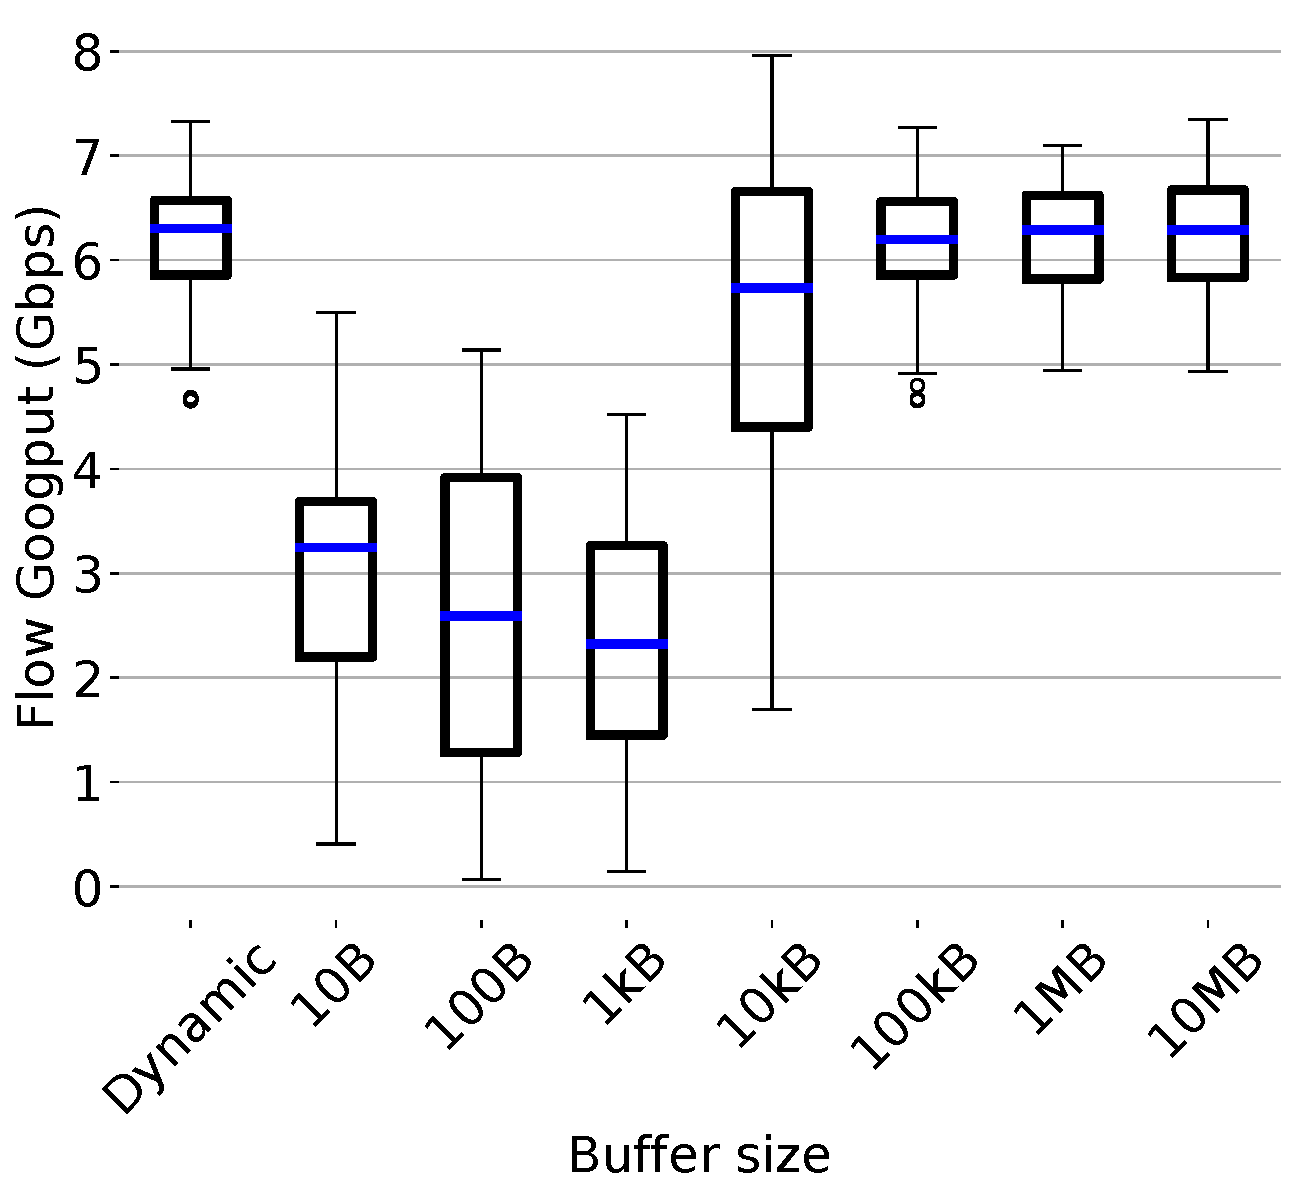
\includegraphics[width=1\linewidth]{figs/tso_gput.pdf}
% 		\caption{IPerf flow goodput}
% 		\label{fig:offload_latency1}
% 	\end{subfigure}
% 	\begin{subfigure}[t]{.45\linewidth}
% 		\centering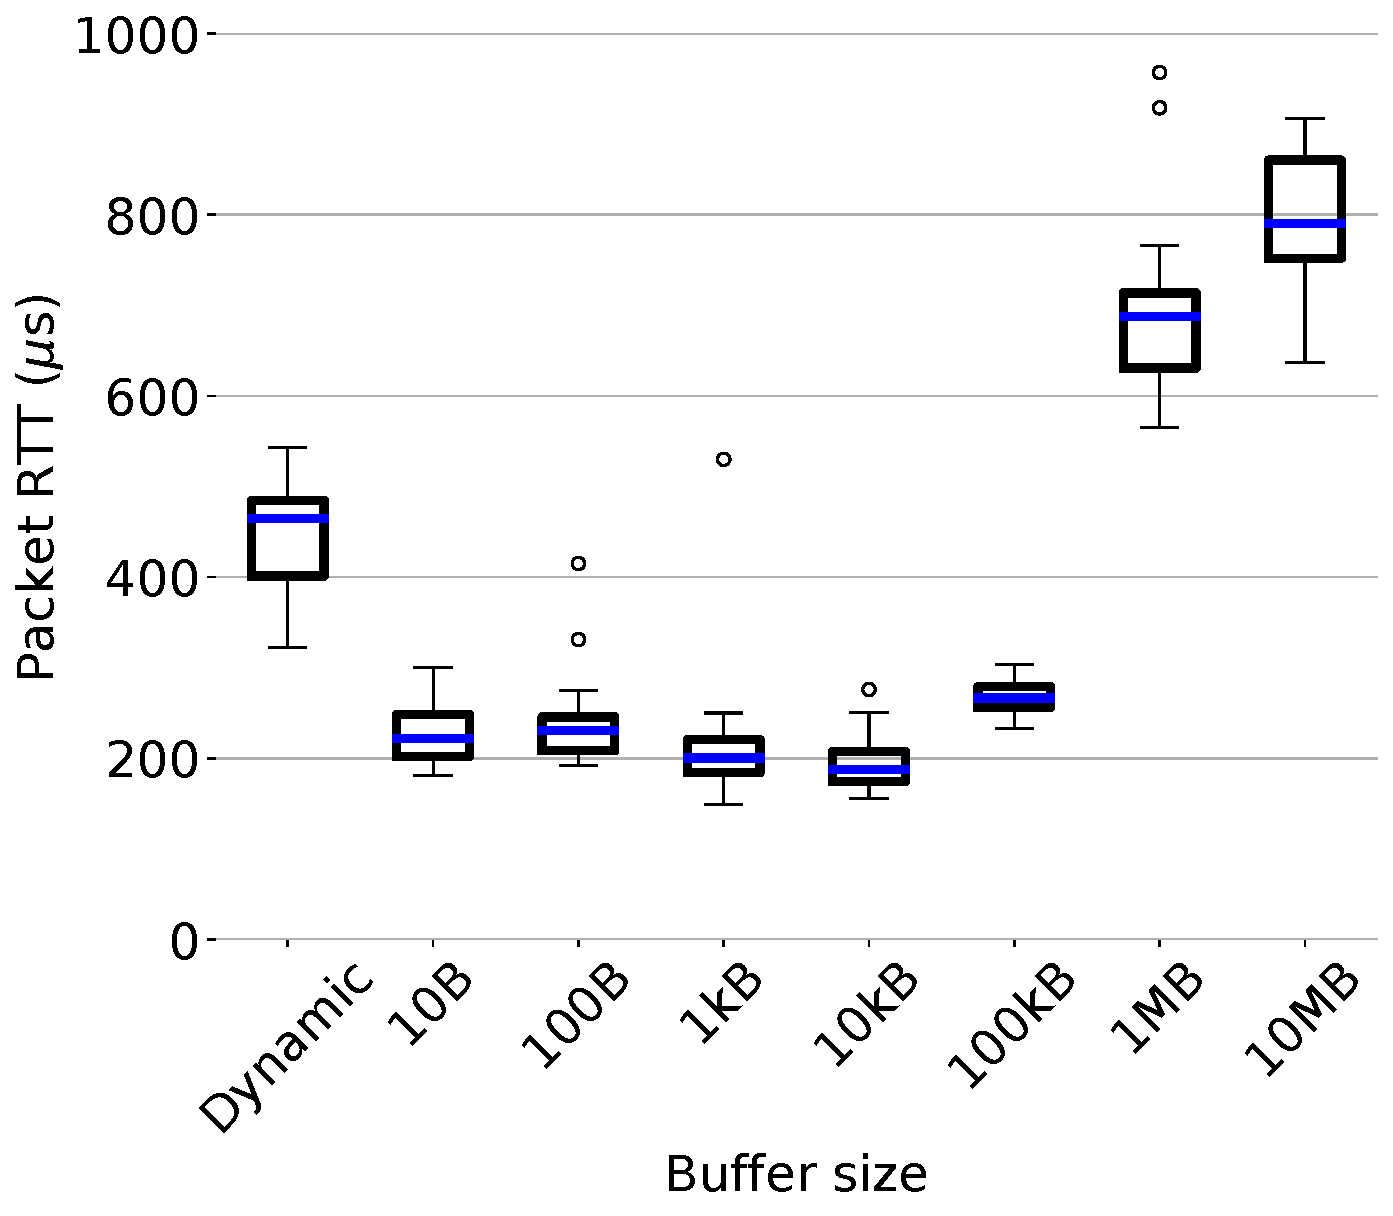
\includegraphics[width=1\linewidth]{figs/tso_rtt.pdf}
% 		\caption{Iperf RTTs}
% 		\label{fig:offload_latency2}
% 	\end{subfigure}
% 	\vspace{-4mm}
% 	\caption{\small{Larger driver rings produce a higher throughput at the expense of higher packet RTTs.}} 
% 		\label{fig:bql_latency}
% 		\vspace{-4mm}
% \end{figure}
\begin{figure}[t]
	\centering
 	\begin{subfigure}[t]{.26\linewidth}
	\centering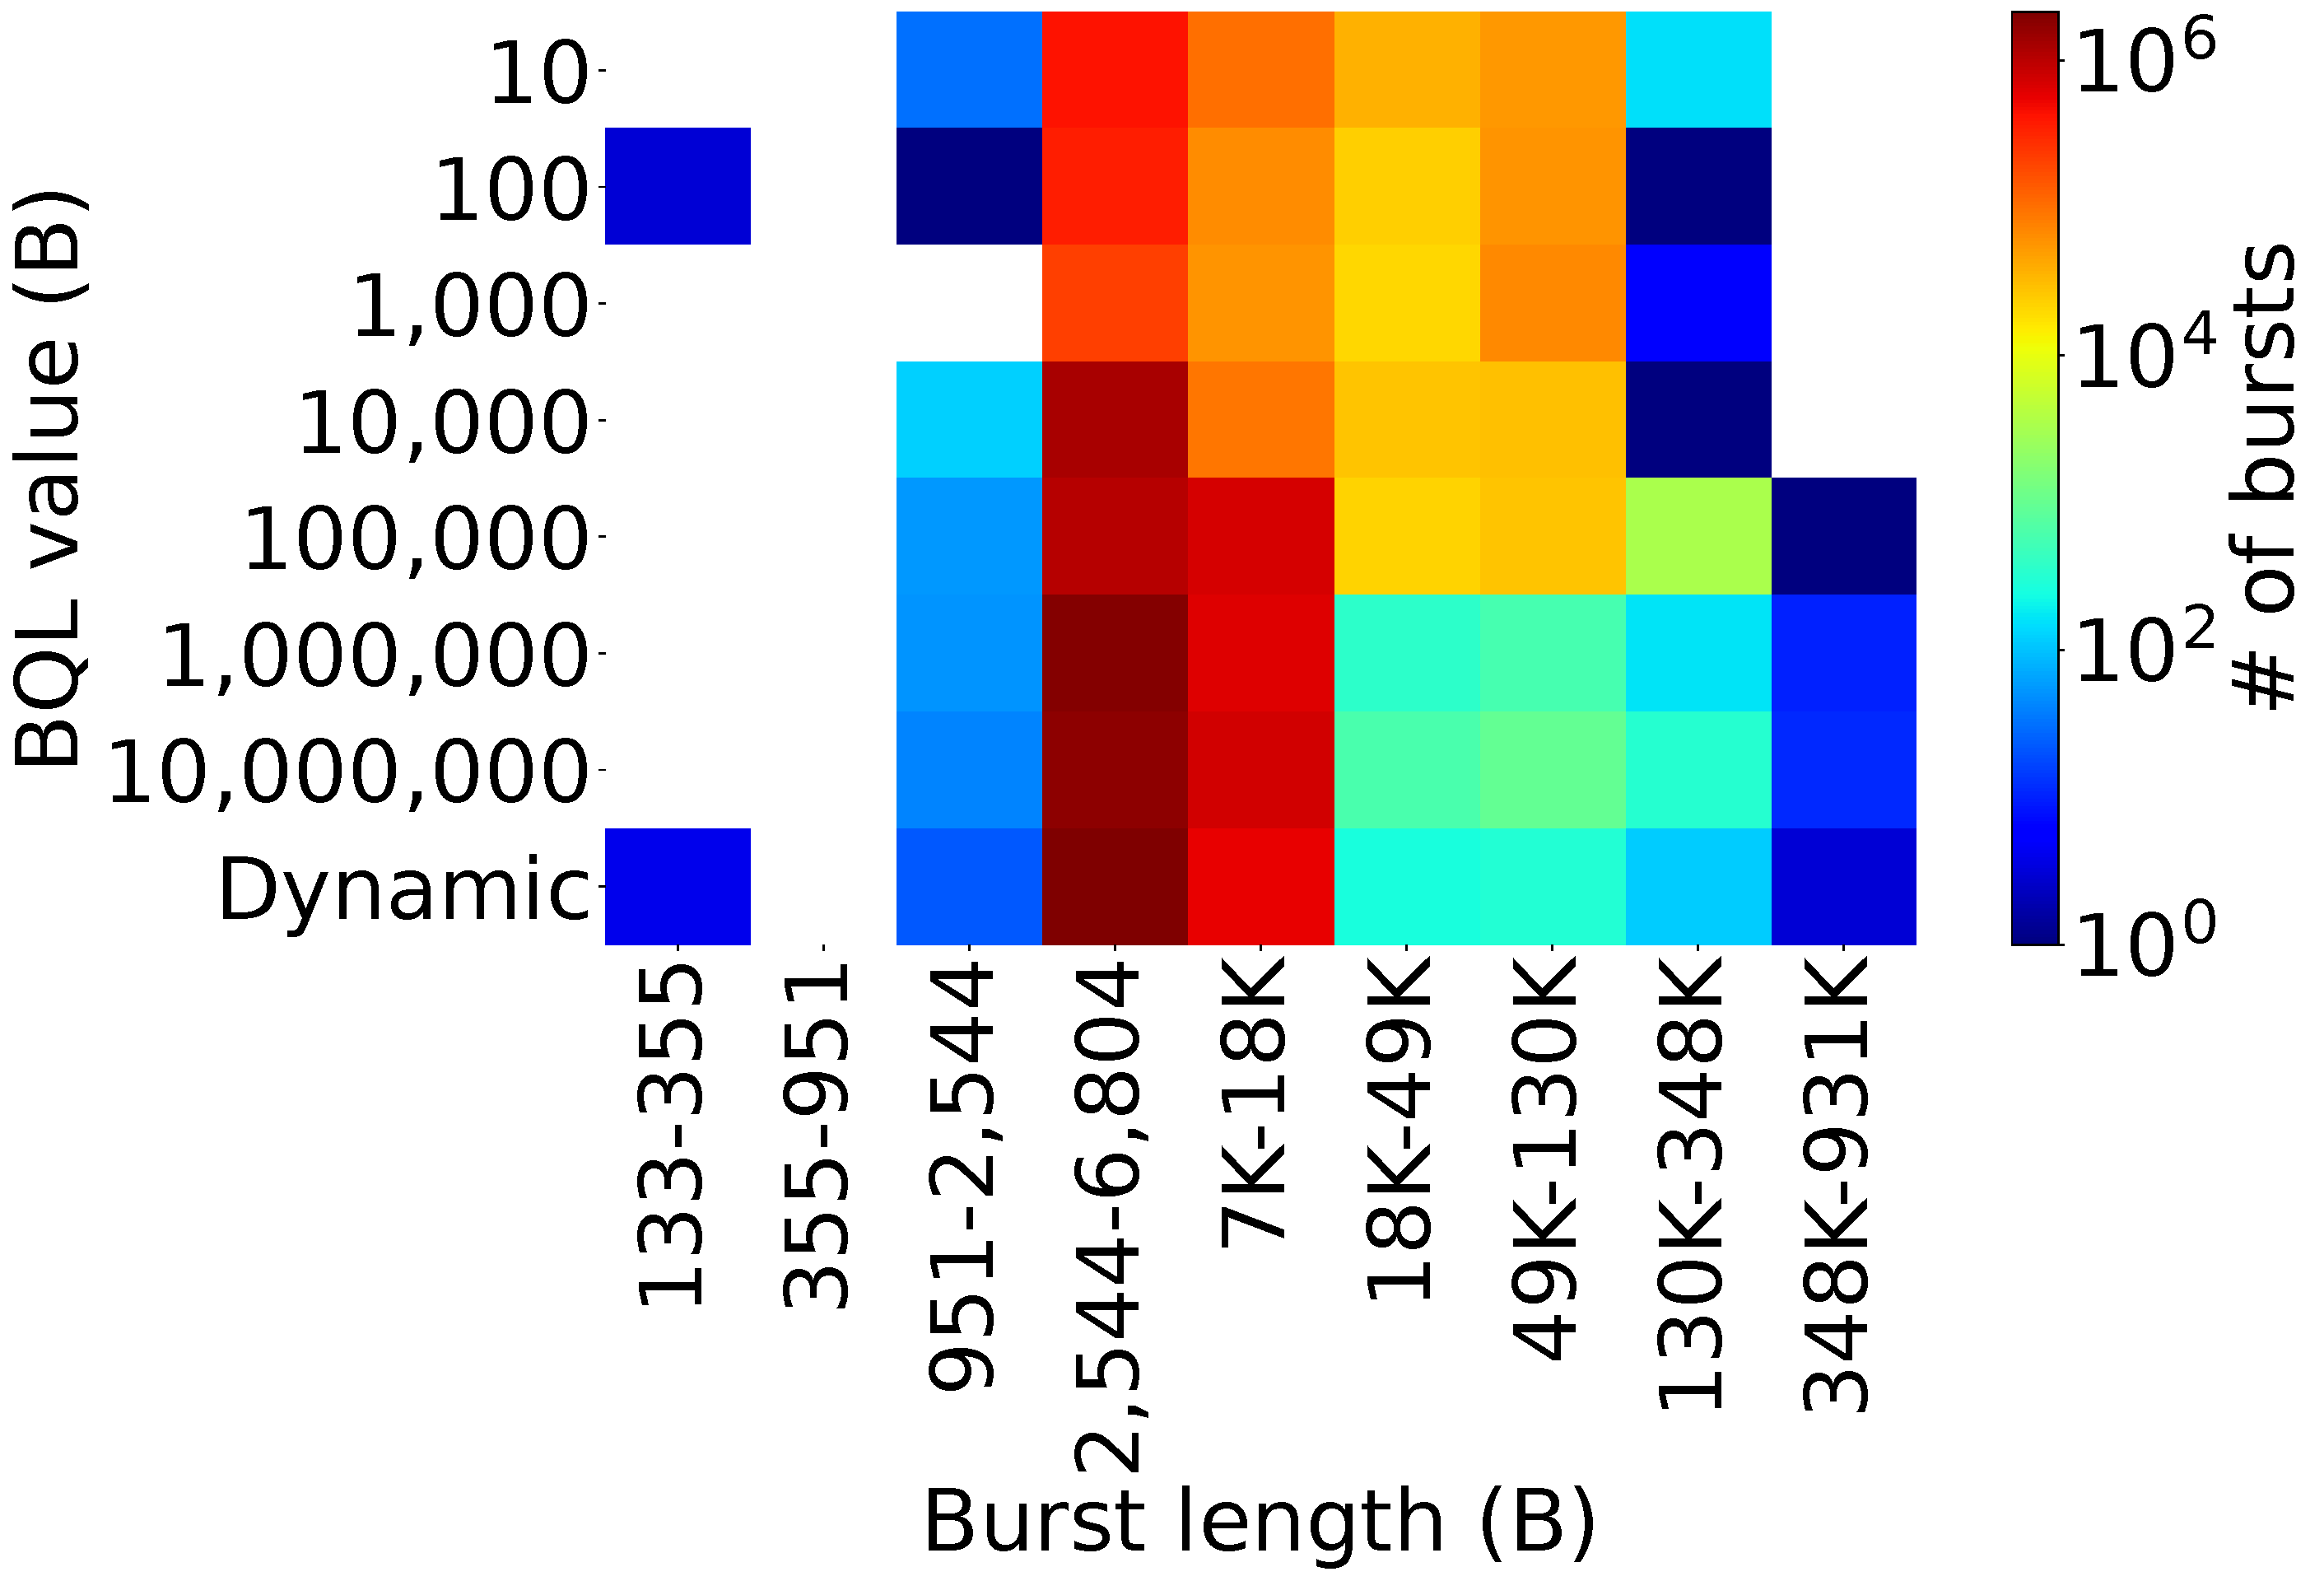
\includegraphics[width=1\linewidth]{figs/bql1.pdf}
			\vspace{-2mm}
	\caption{Burst heatmap}
    \label{fig:bql}
    \end{subfigure}
	\begin{subfigure}[t]{.26\linewidth}
	\centering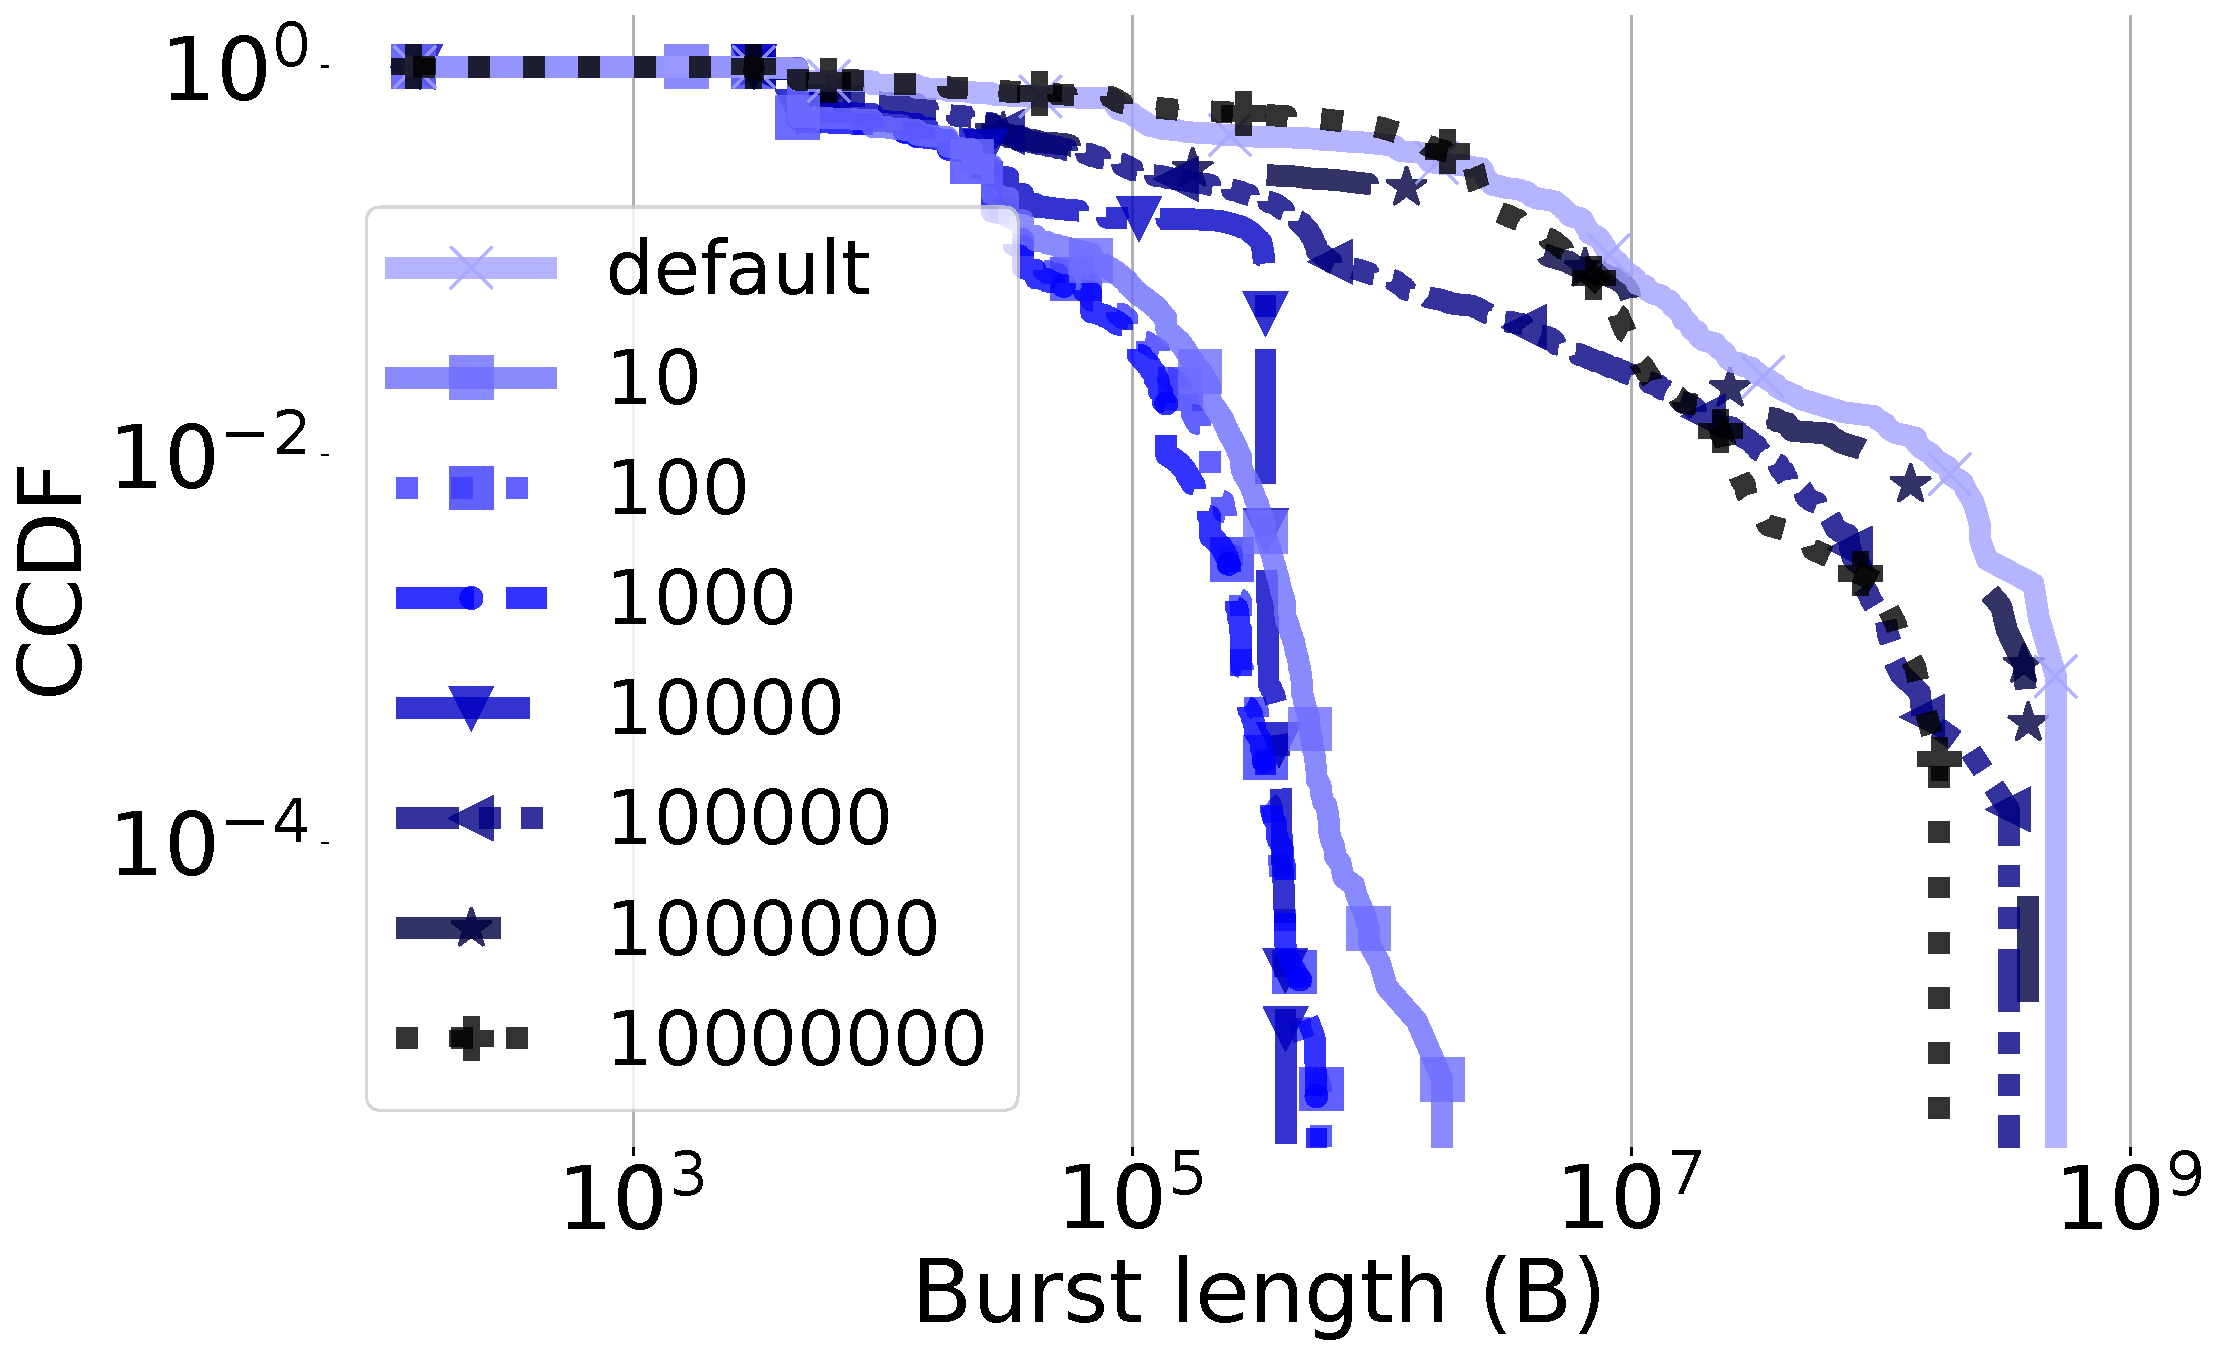
\includegraphics[width=1\linewidth]{figs/bqlccdf_testbed.pdf}
			\vspace{-2mm}
	\caption{Microburst CCDF}
    \label{fig:bql-ccdf}
    \end{subfigure}
    	\begin{subfigure}[t]{.22\linewidth}
		\centering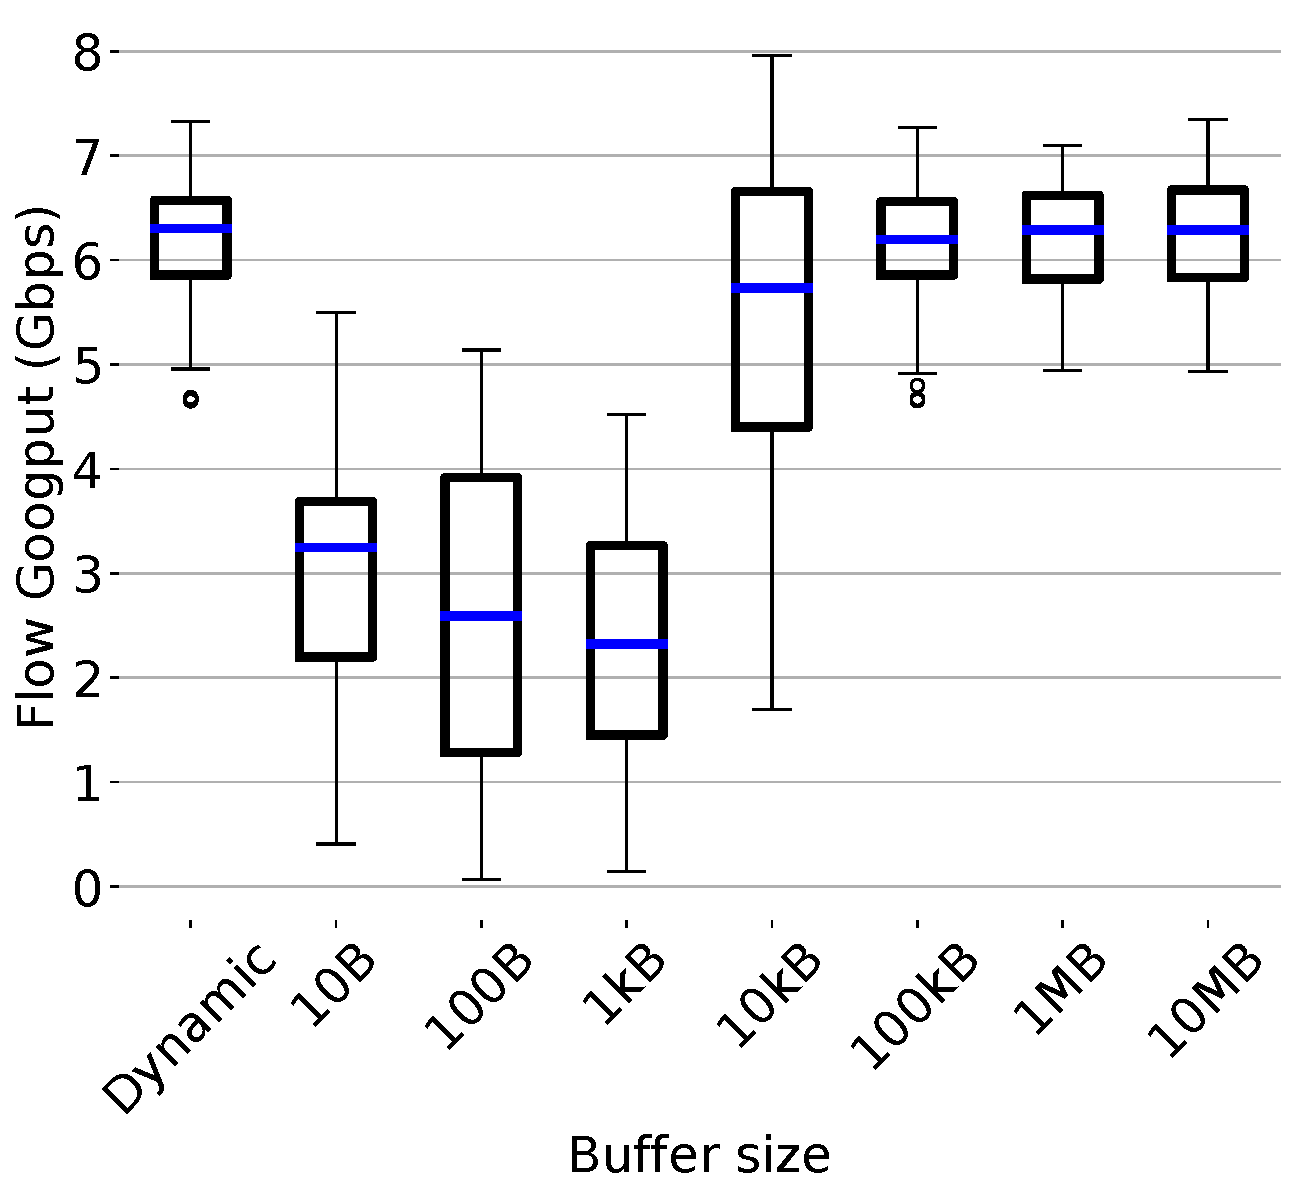
\includegraphics[width=1\linewidth]{figs/tso_gput.pdf}
        \vspace{-2mm}
		\caption{Flow goodput}
		\label{fig:offload_latency1}
	\end{subfigure}
	\begin{subfigure}[t]{.22\linewidth}
		\centering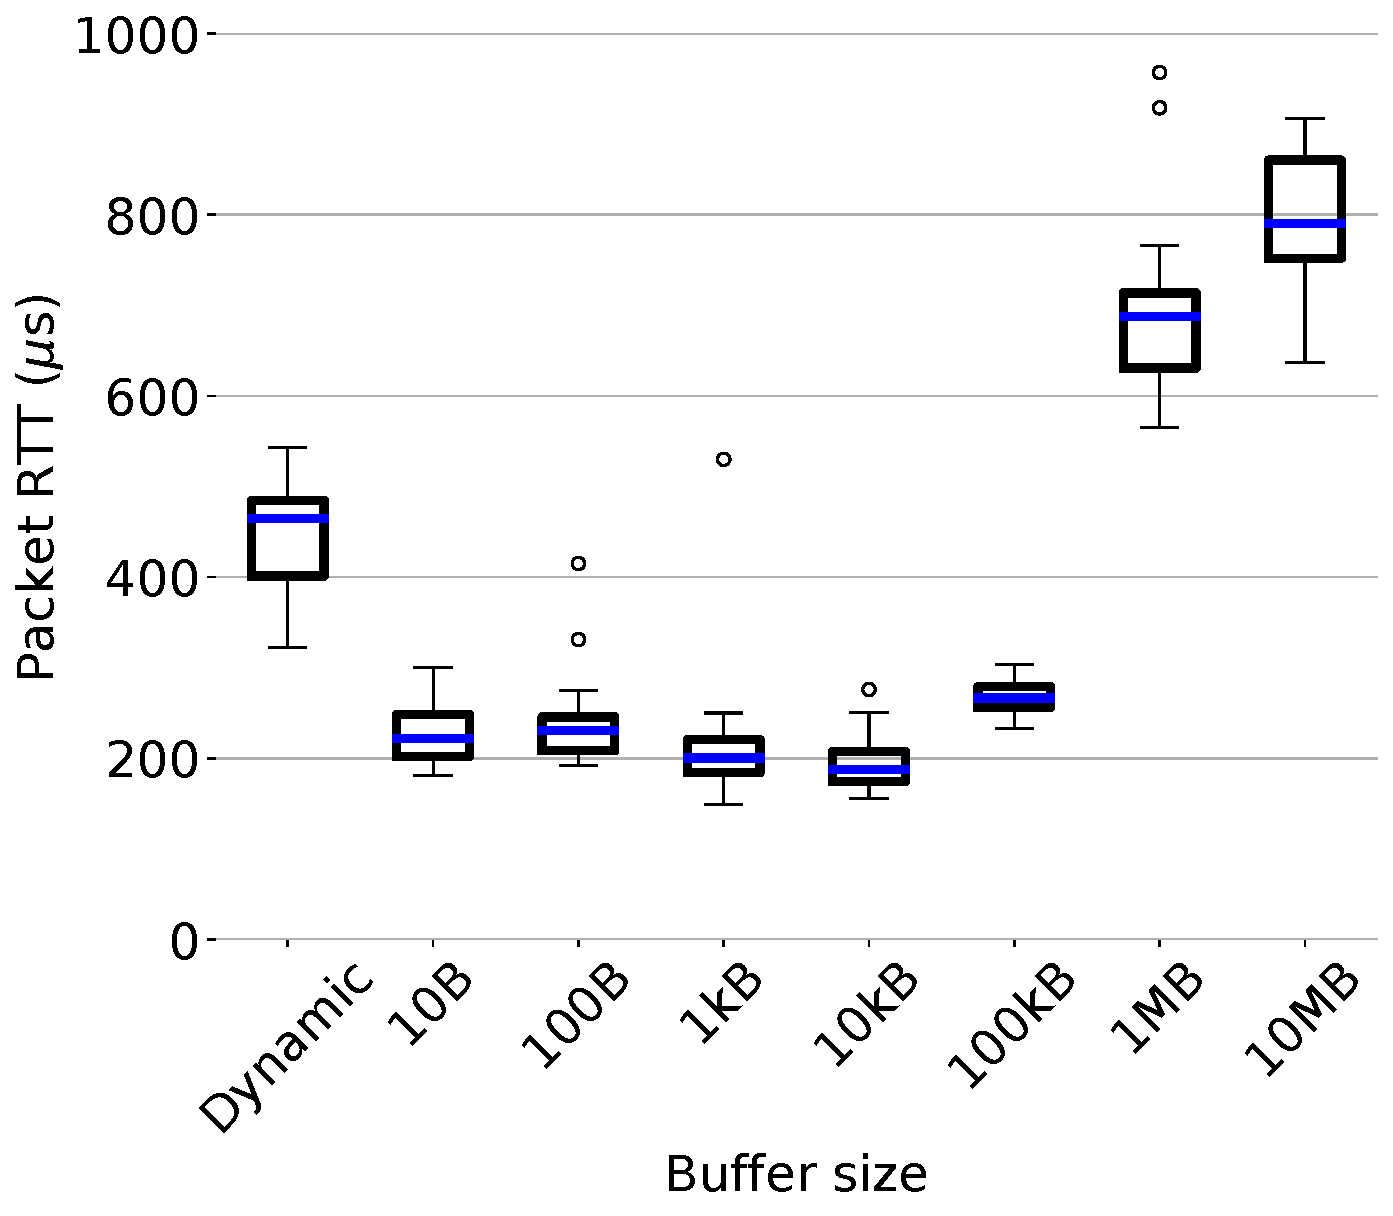
\includegraphics[width=1\linewidth]{figs/tso_rtt.pdf}
        \vspace{-2mm}
		\caption{Packet RTTs}
		\label{fig:offload_latency2}
	\end{subfigure}
% \vspace{-2mm}
	\caption{\small{Larger BQL settings produce longer bursts. Also, the dynamic BQL algorithm presents a similar behavior to a large static ring size.}}
		\label{fig:bql_all}
% 	\vspace{-1em}
\vspace{-2mm}
\end{figure}

Linux kernel employs buffers at various stages of network stack processing to streamline the data movement among various components. The NIC driver queue is the last buffering stage before triggering the hardware. A fixed-size driver queue (a.k.a., TX ring) would ensure that the NIC can always find ready-to-send packets without communicating with the OS. However, due to the unpredictable size of packet buffers in the Linux kernel (ranging from 64B up to tens of kilobytes), the queueing time will considerably add to the overall RTT of packets. To prevent that, OS developers propose a dynamic bound on TX rings that adjusts the limit based on NIC's transmission rate and the availability of data in the TX rings \cite{bql}. To that end, after every transmission, BQL uses time intervals to check whether the NIC was starved in previous transmissions. If the NIC was not fully utilized during any interval while data was available at higher layers, the BQL algorithm increases the limit on the TX ring. Otherwise, if the NIC was fully busy, the BQL is decreased to reduce the queueing overheads. Enforcing smaller queue limits also ensures that the main queuing occurs at the qdisc-level where more advanced queuing disciplines can be employed.

Apart from Linux, NIC buffer sizing is also an important consideration for kernel-bypass runtimes that are less inclined to distribute TX processing among multiple ring buffers \cite{shenango,tas}. Figure \ref{fig:bql_all} demonstrates the impact of driver queue size on performance and burstiness. Intuitively, as we increase the size of the driver's buffer, we greatly increase the queueing time experienced by egress traffic, therefore, preventing the bursts of packets from arriving at the NIC. On the other hand, a larger driver queue is more prone to creating longer bursts as it is more susceptible to triggering segmentation offload (99$^{th}$ percentile burst length for 1 KB buffers and 1 MB buffers are 68 KB and 9 KB, respectively, but 99.99$^{th}$ lengths shift to 68 KB and 86 KB, respectively). The microburst length distributions in Figure \ref{fig:bql-ccdf} further suggest that the default dynamic buffer sizing algorithm tends to maintain larger ring buffers which leads to longer bursts.


\subsubsection{Linux process scheduling}
Apart from the network stack, the operating system features various internal components that might change the traffic shape. For example, Linux offers a range of process scheduling classes suited for various use cases:
\\
\textbf{Completely Fair Scheduler (CFS)} is the default process scheduling class in Linux which aims at achieving fairness among active processes in the system while maintaining responsiveness for I/O-bound applications. when running a mix of compute-intensive and network-intensive workloads, CFS attempts to proportionally share the CPU among workloads leading to longer response times \cite{tales}.
\\
\textbf{Real-time scheduler} supports two policies: \textit{Round-robin} and \textit{First-In-First-Out (FIFO)} scheduling. Both policies give strict priority to I/O-bound applications (if configured properly). By default, the round-robin policy preempts high-priority processes every 100ms while the FIFO policy is non-preemptive. We also deploy Microquanta \cite{snap,microquanta} a semi-real-time scheduling class with microsecond time precision.
% \textbf{Microquanta scheduler} is a more recent attempt at introducing process schedulers with microsecond time precision. Microquanta was introduced as part of Snap microkernel \cite{snap} to allow fine-grained time accounting among userspace processes as well as among real-time and non-real-time applications. We deploy a publicly available implementation of Microquanta on our testbed and configure it to switch between available processes in 50$\mu$s intervals. We also adjust the CPU time allocation between background and network apps to 4-1. This means that Microquanta will allocate 80\% of its time window to the higher-priority network processes.
\begin{figure}[t]
\centering
% \begin{subfigure}[t]{0.8\linewidth}
%     \centering
%     	\includegraphics[width=1\linewidth]{figs/sched_hurst.pdf}
%          \caption{\small{\textbf{Hurst estimates for different process schedulers}}}
% 	\label{fig:sched-hurst}
% \end{subfigure}
\begin{subfigure}[t]{0.90\linewidth}
    \centering
    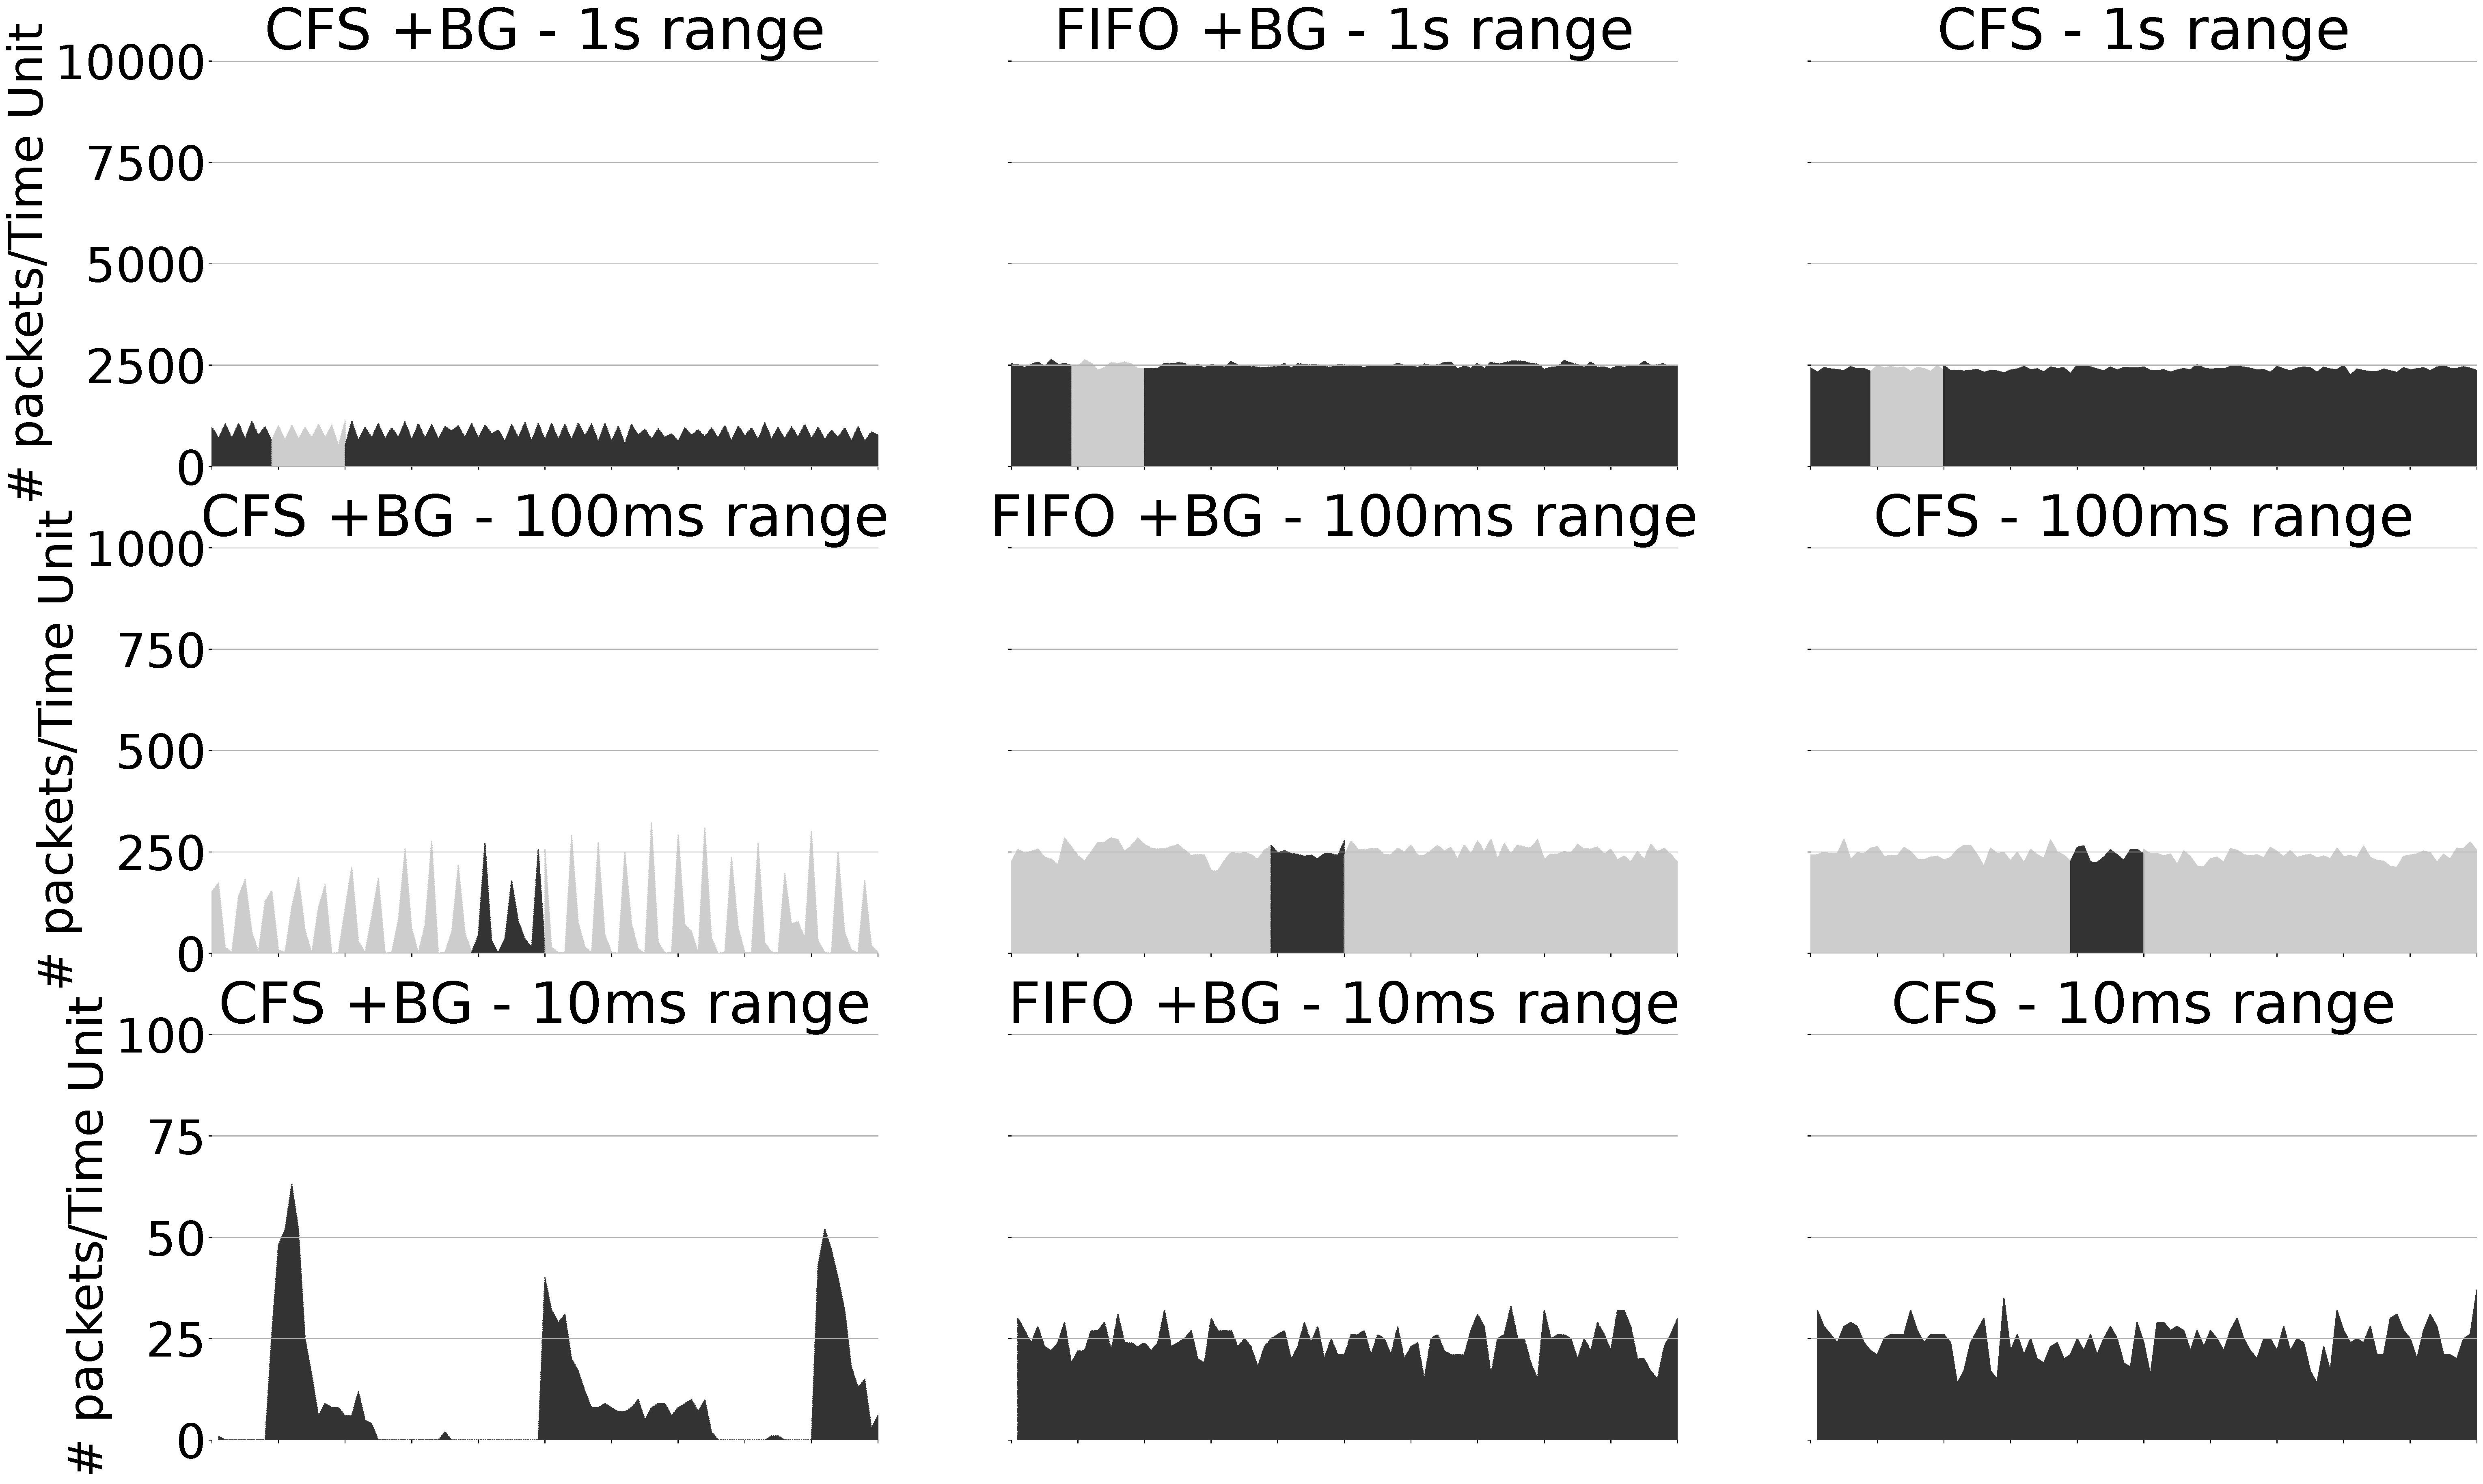
\includegraphics[width=1\linewidth]{figs/sched_ts.pdf}
 %    \caption{\small{\textbf{Timeseries of packet arrivals}}}
	% \label{fig:sched-ts}
\end{subfigure}
\vspace{-1mm}
    \caption{\small{Impact of process scheduling on traffic bursts.}}
	\label{fig:sched}
 \vspace{-2mm}
\end{figure}

Valinor's picture of traffic burstiness is consistently similar when  the network application is running alone as Hurst estimates vary between 0.51 and 0.54 for all the schedulers. However, when the background process is introduced, a course-grained process scheduler like CFS must enforce fair CPU time sharing, resulting in the leap of its H estimate to 0.74 while other schedulers are able to schedule the network application's threads in short timescales and result in smooth transmissions. To validate the self-similarity estimates, we plot the time series of CFS (running only the network workload), CFS+BG (running the network workload alongside background threads), and the real-time FIFO scheduler running both applications (FIFO+BG) in Figure \ref{fig:sched}. The self-similar nature of the CFS+BG scenario is noticeable in the leftmost column as CFS causes the network packets to be sent in larger chunks, causing intermittent but larger bursts at short time spans.

\section{Conclusions}
\label{sec:valinor-conclusion}

We presented the design of Valinor, a burst measurement framework that consists of an in-host eBPF framework and an in-network timestamping module for programmable switches. Valinor can capture burstiness at different scales (ranging from nanoseconds to seconds).
We use Valinor to demonstrate how host networking elements affect bursts. 
We show that the scaling behavior of traffic at long timescales and burstiness at fine timescales vary significantly across different host networking configurations (process schedulers, congestion control algorithms, single vs. multi-queue NICs, etc.) and across different classes of practical workloads. In particular, we show the impact of hardware-resident functions (e.g., NIC schedulers) that are largely overlooked in characterizing burstiness. 
%Leveraging this ability, we use theoretical models of burstiness, like rescaled-range analysis, to show the impact of NIC scheduling, TCP segmentation offload, transport protocols, and process scheduling on burstiness. 
This variability of burstiness and the implications of bursts on performance underscore the need for  measurement systems to perform periodic burst analysis.
\chapter{Self-Clocked Round-Robin Packet Scheduling for Better Burst Control} \label{chap:chap-3}


% epigraph after chapter heading
% \epigraph{The unavoidable price of reliability is simplicity.}{-- C. A. R. Hoare}


%%%% MUST: add the citation for the chapter if it is a reprint


\section{Packet Scheduling for Modern Internet}
\label{sec:scrr-background}

% Deficit Round Robin \cite{drr} has emerged as one of the best compromise among packet schedulers, due to its fairness, low complexity and its compatibility with any transport and any traffic. We argue that Deficit Round Robin is no longer suited for the mixed Internet workloads that consist of heavy, throughput-intensive flows, as well as bursty latency-sensitive flows.
Internet workloads incorporate a mix of heavy, throughput-intensive flows, as well as bursty latency-sensitive flows with diverse arrival patterns. Can Deficit Round Robin \cite{drr}, as the de facto candidate for fair scheduling cope with modern traffic characteristics?



\subsection{A Brief History of Packet Scheduling}
\label{sec:schedulers}

Historically, Packet-by-packet Generalized Processor Sharing (PGPS) \cite{gps} was among the first scheduling paradigms that target fair bandwidth allocation among tenants. Tenants or flows are classified into separate FIFO queues that are then processed by the packet scheduler. Subsequently, numerous Fair Queuing schedulers \cite{sparrow,scfq,stfq,frr,drr,mqfq,wfq} were introduced with distinct bounds and computational complexities. 
Classical Fair Queuing algorithms such as Start-Time Fair Queuing (STFQ) \cite{stfq} have the downside of expensive per-packet sorting operations as they need to constantly track and update the bandwidth allocation for each flow and choose the most eligible sub-queue, i.e., the sub-queue with the least progress. Further, computing requirement scales up with the number of sub-queues.

Deficit Round Robin (DRR) scheduling addresses this shortcoming by
allowing constant complexity dequeue operations irrespective of scale
\cite{drr}. Instead of maintaining a sorted data structure to keep
track of flow progress, it visits each sub-queue in a round-robin
fashion and allocates a fixed amount of bytes, called
\textit{quantum}, to each queue at each round. The part of the quantum
that is too small to send the next packet is accumulated as a deficit
for the queue.
Other variants of DRR, including Weighted Round-Robin (\textit{WRR}) and
Modified Deficit Round Robin (\textit{MDRR}) \cite{cisco} can operate on
a limited number of FIFO queues strictly reserved for different flow
priorities \cite{intel810}. These variants have a coarser fairness
granularity (per priority group, instead of per-flow) and need to be
configured with a deficit value that determines the amount of bytes
each priority group transmits on each pass.

Due to its constant computational complexity and low memory footprint,
\textit{DRR} is one of the most widely deployed packet schedulers in both
software and hardware \cite{drr,loom,cisco,juniper,tc,pifo,intel810,intel710}.
Even with the emergence of novel queuing abstractions such as \textit{PIFO}
\cite{pifo} and calendar queues \cite{calendar} that offer advanced
traffic classification and shaping, \textit{DRR} endures as a robust and widely
used option for flow scheduling, particularly in scenarios where
intricate packet classification is unnecessary
\cite{demi,netchannel,corundum,justitia,sch-fq} and standard TCP
support is required.\footnote{We later compare the performance of
state-of-the-art implementations of \textit{PIFO}, such as AIFO \cite{aifo} and
\textit{SP-PIFO} \cite{sppifo}, with \textit{DRR} in \S\ref{sec:scrr-evaluation}. Our results
suggest that \textit{AIFO} suffers from severe throughput loss at large RTTs,
while \textit{SP-PIFO} causes heavy packet re-ordering.}

\begin{figure*}[t]
 \centering
\begin{subfigure}[t]{.24\linewidth}
    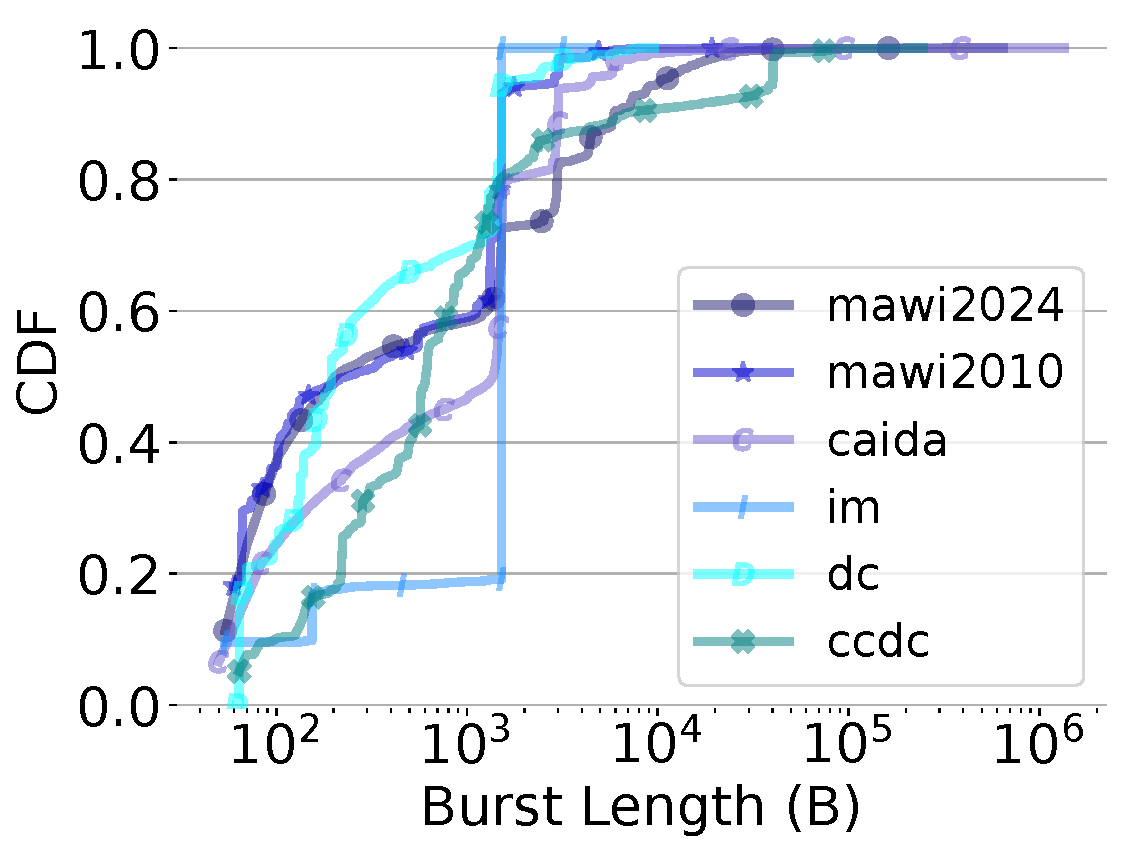
\includegraphics[width=\linewidth]{figs/aggregate_ipg_burstsize_cdf_10.pdf}
    \vspace{-6mm}
 \end{subfigure}
\begin{subfigure}[t]{.24\linewidth}
 \centering
    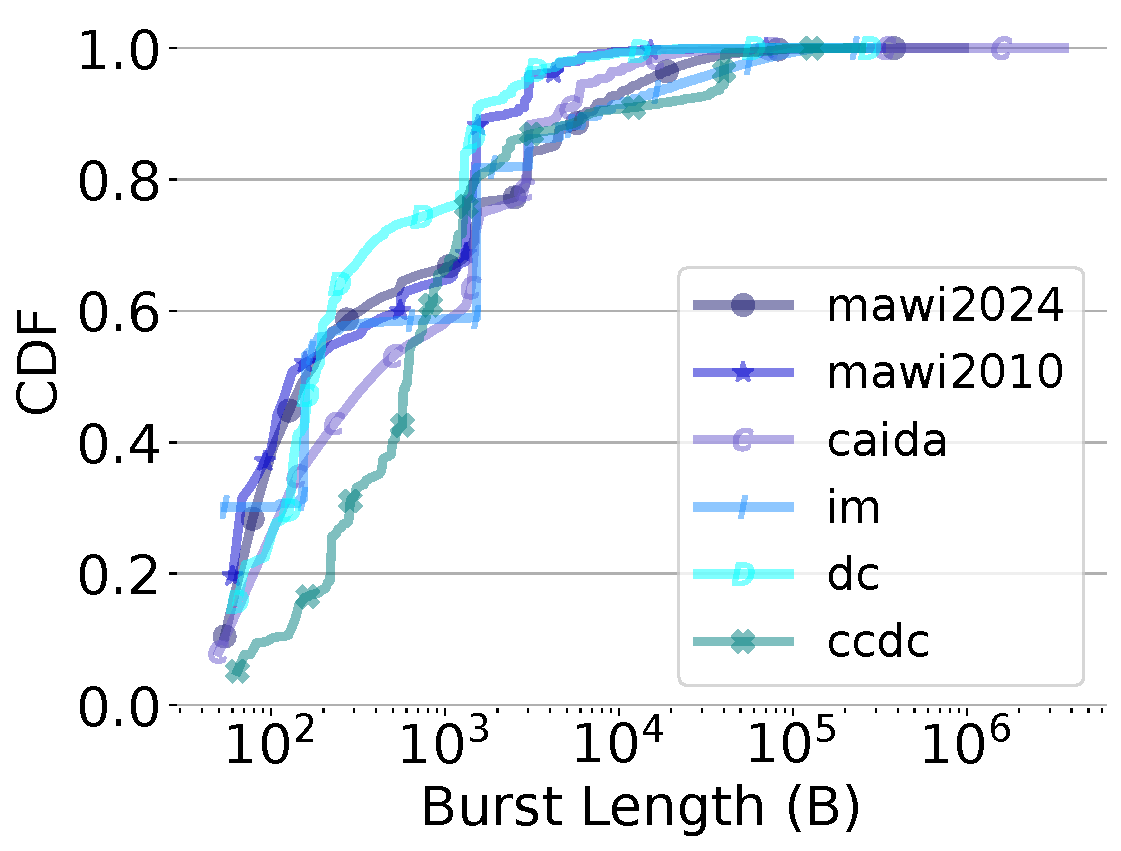
\includegraphics[width=\linewidth]{figs/aggregate_ipg_burstsize_cdf_50.pdf}
    \vspace{-6mm}
\end{subfigure}
\begin{subfigure}[t]{.24\linewidth}
 \centering
 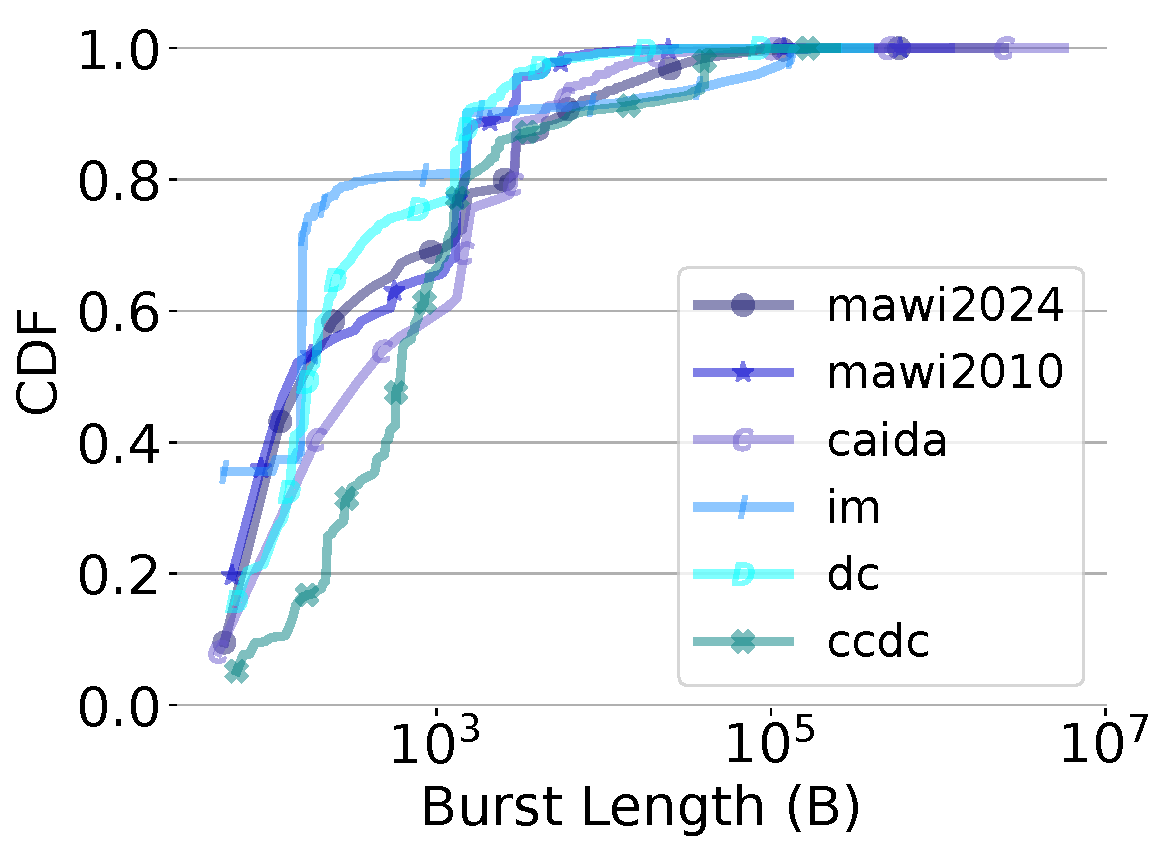
\includegraphics[width=\linewidth]{figs/aggregate_ipg_burstsize_cdf_100.pdf}
    \vspace{-7mm}
 \end{subfigure}
 \begin{subfigure}[t]{.24\linewidth}
 \centering
        \centering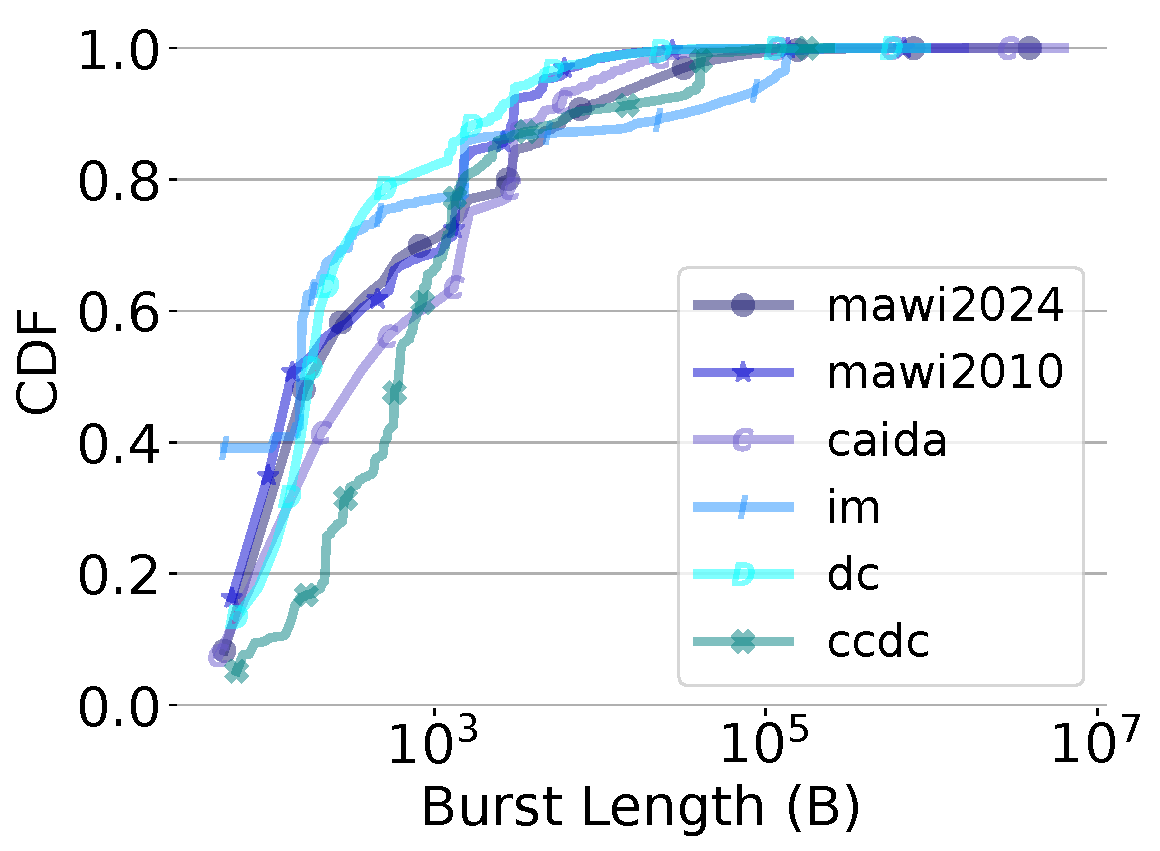
\includegraphics[width=1\linewidth]{figs/aggregate_ipg_burstsize_cdf_500.pdf}
         \vspace{-7mm}
\end{subfigure}
\begin{subfigure}[t]{.24\linewidth}
    \includegraphics[width=\linewidth]{figs/aggregate_ipg_burstsize_pkt_cdf_10.pdf}
    \vspace{-6mm}
    \caption{\small{\textit{IPG < 10$\mu$s}}}
 \end{subfigure}
\begin{subfigure}[t]{.24\linewidth}
 \centering
    \includegraphics[width=\linewidth]{figs/aggregate_ipg_burstsize_pkt_cdf_50.pdf}
    \vspace{-6mm}
    \caption{\small{\textit{IPG < 50$\mu$s}}}
\end{subfigure}
\begin{subfigure}[t]{.24\linewidth}
 \centering
 \includegraphics[width=\linewidth]{figs/aggregate_ipg_burstsize_pkt_cdf_100.pdf}
    \vspace{-6mm}
    \caption{\small{\textit{IPG < 100$\mu$s}}}
 \end{subfigure}
 \begin{subfigure}[t]{.24\linewidth}
 \centering
        \centering\includegraphics[width=1\linewidth]{figs/aggregate_ipg_burstsize_pkt_cdf_500.pdf}
         \vspace{-6mm}
		\caption{\small{\textit{IPG < 500$\mu$s}}}
\end{subfigure}
  \vspace{-0.3cm}
    \caption{\small{Burst length distribution for Internet traces using various IPG thresholds.}}
    \label{fig:traces-all}
  \vspace{-0.2cm}
\end{figure*}


\subsection{Flow Burstiness in Modern Traffic}

Burstiness is a well-known phenomenon for Internet traffic due to its multitude of root causes \cite{wild,bullet,why,im,valinor,high-resolution}. The emergence of interactive applications such as cloud gaming, video streaming, and video conferencing further underscores a type of traffic that experiences long idle times due to user behavior, network congestion, and variable bit-rate enforcement by the application \cite{im,movidiff,passive,qoe,gaming}. Traffic studies further report that many latency-sensitive workloads primarily produce short flows. For example, the median response size for web requests entering Facebook data centers is reported to be less than 10 kilobytes \cite{edge}, and frames in Zoom video traffic do not exceed 10 kB, with large gaps in between \cite{passive}. 
% The Inter-Packet Gap (IPG) distribution of Internet traces \cite{caida} in Fig \ref{fig:caida} further certify the existence of large gaps among packets of a flow.

A burst is a train of packets with inter-packet gaps smaller than a threshold \cite{bullet}. Using this definition, we plot the CDF of burst lengths for six representative Internet traces. These traces include backbone internet (\textit{caida}) \cite{caida} traces dating to 2019, campus network traces (\textit{dc}) \cite{wild}, ISP gateway traces for 2010 and 2024 (\textit{mawi}) \cite{mawi}, instant messaging (\textit{im}) \cite{im} packet traces and anonymized traces using in cyber defense competitions (\textit{ccdc}) \cite{ccdc}. According to Figure \ref{fig:traces-all}, regardless of the configured threshold, a diverse range of burst lengths can be observed which suggests that Internet workloads feature both heavily backlogged and short flows arriving at the bottlenecks. In fact. the similarity among burst size distributions with different IPG thresholds suggest that our analysis of Internet bursts is independent of the chosen threshold. Additionally,  the diversity in burst sizes suggests that not all Internet flows tend to remain active for a long time as they arrive at a bottleneck. Notably, many flows exhibit small bursts of packets followed by large idle periods. But we also see a number of very large bursts belonging to heavy flows likely to congest the packet scheduler.
Figure \ref{fig:trace-hurst} compares the hurst estimate (\S\ref{sec:valinor-background}) for the above traces. As previous studies point \cite{high-resolution}, network traffic is bursty and unpredictable for the most part. A small portion of traffic exhibits a strong self-similarity which suggests persistent burstiness at different timescales. These flows usually create backlogged queues on a fair packet scheduler. On the other hand many of the flows are composed of short bursts that can arrive at any time.

% \begin{figure*}[t]
%      \begin{minipage}[t]{0.21\textwidth}
%    	 \centering
%     \includegraphics[width=\linewidth]{figs/aggregate_ipg_burstsize_p99.pdf}
%     \vspace{-6mm}
%     \caption{\small{\textit{p99 of burst sizes with different IPG thresholds shows various levels of burstiness. \todo{a 4 by two figure grid}}}}
% 	\label{fig:bursts-wild}
%   \end{minipage}
%        \hfill
%          \begin{minipage}[t]{0.18\textwidth}
%    	 \centering
%     \includegraphics[width=\linewidth]{figs/pkt_num_lat_cn_2t4x16_mn_2tb2x4_mss_150_bql_9k_comp.pdf}
%     \vspace{-6mm}
%     \caption{\small{\textit{DRR offers poor application performance under different burst sizes. \todo{a simplified version of the figure (170s)}}}}
% 	\label{fig:drr-burst-latency}
%   \end{minipage}
%   \hfill
%       \begin{minipage}[t]{0.20\textwidth}
%     \centering
%     \includegraphics[width=1\linewidth]{figs/burst_cn_2t4x8_mn_2tb2x4_css_500_kp_lat_fq_drr.pdf}
%     \vspace{-6mm}
%     \caption{\small{\textit{Quantum in DRR trades-off CPU for better scheduling latency.}}}
% 	\label{fig:quanta-cpu-lat}
%   \end{minipage}
%   \hfill
%    \begin{minipage}[t]{0.19\textwidth}
%    		\centering\includegraphics[width=1\linewidth]{figs/cpu_bandwidth.pdf}
%          \vspace{-6mm}
% 		\caption{\small{\textit{Increased CPU utilization quickly results in reduced bandwidth.}}}
%             \label{fig:cpu-bw}
%   \end{minipage}
%    \begin{minipage}[t]{0.19\textwidth}
%    		\centering\includegraphics[width=1\linewidth]{figs/workload_dists.pdf}
%          \vspace{-6mm}
% 		\caption{\small{\textit{Packet length distributions in the wild is diverse and skewed.}}}
%             \label{fig:packets-wild}
%   \end{minipage}
%   \hfill
%   \vspace{-0.5cm}
% \end{figure*}

\begin{figure*}[t]

 \centering
  \begin{minipage}[t]{0.32\textwidth}
   	 \centering
    \includegraphics[width=\linewidth]{figs/hursts.pdf}
    \vspace{-7mm}
    \caption{\small{Hurst estimates for public packet traces.}}
	\label{fig:trace-hurst}
  \end{minipage}
  \begin{minipage}[t]{0.32\textwidth}
   	 \centering
    \includegraphics[width=\linewidth]{figs/pkt_num_lat_cn_2t4x16_mn_2tb2x4_mss_150_bql_9k_comp_fah.pdf}
    \vspace{-7mm}
    \caption{\small{DRR offers poor latency under different burst sizes.}}
	\label{fig:drr-burst-latency}
  \end{minipage}
  % \hfill
   \begin{minipage}[t]{0.32\textwidth}
     		\centering\includegraphics[width=1\linewidth]{figs/aggregate_ipg_pktsize_cdf.pdf}
         \vspace{-7mm}
		\caption{\small{Skewed packet length distributions in the wild.}}
            \label{fig:packets-wild}
  \end{minipage}
  \vspace{-0.2cm}
\end{figure*}
 


DRR has effectively the same theoretical bounds as Fair Queuing
schedulers (\S\ref{sec:schedulers}): it is fair and has a maximum
service deviation of 2$\times$ the quantum \cite {drr}. The fairness,
burstiness and latency guarantees of \textit{DRR} and Fair Queuing schedulers
are based on the assumption that all flows arriving at the scheduler
are always backlogged \cite{drr,scfq,stfq}. Alas, the above evidence
suggests that this is rarely the case for modern Internet traffic!
In practice, DRR usually has higher latency for those short bursty
flows which are not backlogged at the scheduler, and this is seldom
studied. With gaps in arrivals, short flows are prone to get stuck
behind backlogged flows in the scheduler.
Figure \ref{fig:drr-burst-latency} compares the response times for
a request-response workload under two software implementations of
\textit{DRR}, the original design presented in \cite{drr}, and the
state-of-the-art implementation of \textit{DRR} which implements \textit{Sparse
Flow Optimization (SFO)} \cite{sfo}, a technique that prioritizes
interactive traffic (\S\ref{sub:sfo}). We compare \textit{DRR} with two
different quantum settings: 1500B and 9000B, and with \textit{STFQ}
\cite{stfq}. Two senders generate a total of 16 parallel streams of requests
composed of bursts of 150B MSS packets, while the burst length increases on the x axis. Two other senders
generate 64 heavy flows each to ensure the scheduler is backlogged. The full
experiment setup can be found in \S\ref{sec:scrr-eval-latency}. Latency
gaps as large as 4$\times$ between \textit{DRR} and \textit{STFQ}
suggest that \textit{DRR} degrades the application performance due to
poor scheduling decisions regardless of its quantum setting, as
consecutive packets in a burst have to wait for full scheduling rounds
before they are transmitted. \textit{DRR+SFO} is initially able to
bridge this gap by boosting short flows through the scheduler, but as
the burst size increases, consecutive packets of the burst do not benefit from prioritization and have to wait.

%The implications of traffic behavior on packet scheduling warrant a closer study. Fair packet scheduling, often represented by DRR due to its practical implementation, mostly centers around strong fairness, low per-flow burstiness, low computation complexity, and high scalability for packet schedulers deployed in the wild. These characteristics are built based on the assumption that all flows arriving at the scheduler are always backlogged \cite{drr,scfq,stfq}. Alas, the above evidence suggests that this is rarely the case for modern Internet traffic! With gaps in arrivals, short flows are prone to get stuck behind backlogged flows in the scheduler. Fig. \ref{fig:drr-burst-latency} compares the response times for a request-response workload under two implementations of DRR, the original design presented in \cite{drr}, and the state-of-the-art implementation of DRR which separates new incoming flows from old active flows and gives strict priority to new flows in order to improve responsiveness. This mechanism is referred to as Sparse Flow Optimization (SFO) \cite{sfo}. We compare two different quantum settings: 1500B and 9000B with a software implementation of STFQ \cite{stfq} in a setup where we send a burst of 150B MSS packets as the request data. The full experiment setup can be found in \S\ref{evaluation}. The latency gaps as large as 4$\times$ between DRR and STFQ suggest that DRR degrades the application performance due to poor scheduling decisions regardless of its quantum setting as consecutive packets in a burst have to wait for full scheduling rounds before they are transmitted. DRR+SFO is initially able to bridge this gap by boosting short flows through the scheduler, but as the burst size increases, these flows are demoted to old flows and suffer from a similar fate as DRR.


% To demonstrate the impact of flow arrivals in the performance of packet scheduling, we run two separate latency-sensitive workloads, one using TCP cubic flows sending 500B request and response packets, while the other sends ICMP echo flows of similar size on the physical testbed described in \S\ref{sub:eval-gsogro}. The router node runs the original software implementation of DRR \cite{drr} that is also backlogged with 64 concurrent UDP flows that share the same bottleneck link as the latency-sensitive flows. Fig. \ref{fig:ping} presents the mean response times of latency-sensitive flows using lines and the 10th and 90th percentiles of their response times using error bars. Looking at the top lines, as we increase the quantum size for DRR, both workloads experience higher response times. For example, using a 9KB quantum for the backlogged scheduler increases the response times for both TCP and ICMP flows by around 3$\times$. This is because the latency-sensitive flows are delayed by background flows sending larger bursts of packets during their turn. 

% To account for this unwanted latency, recent works introduce \textit{Sparse Flow Optimization (SFO)} for the DRR scheduler by separating the list of new flows and old flows in the scheduler, with strict priority given to the flows that recently become active. SFO has made its way into Linux qdiscs that use DRR \cite{sfo}. We repeat our experiments with SFO and see surprising distinctions between the TCP and ICMP workloads. While the ICMP traffic detangles itself from DRR's quantum configuration, a large majority of TCP flows still experience degraded performance with increased quanta. This is because the gap between the acknowledgement packet and the response data packet is large enough that while the first packet is boosted through the new flows list, the response data packet will arrive after the flow is demoted to the old flows, so it has to wait for a full scheduling round to get serviced \cite{formal}. Unfortunately, resorting to a small quantum to avoid aggravated scheduling delays will violate DRR's theoretical bounds \cite{drr} and result in increased CPU utilization as we observe further in \S\ref{sec:drr-tradeoff}.

% The above findings hint at the presence of two flow categories: \textit{heavy} or \textit{sparse}.
% A \textit{heavy} flow can be identified by its tendency to always being active in the schedule due to having a packet waiting. Workloads such as file transfer and large downloads on the edge, proportions of web traffic, and machine learning and data mining transfers inside and between datacenters are a few examples \cite{deadline,codedbulk,bulk}. \textit{Sparse} flows can be defined as flows that do not use their fair share of bandwidth during a scheduling period, where the fair share is defined as the available capacity divided by (weighted) number of active flows during a period when all active flows are serviced. 
% Sparse flows are common in Internet traffic. Real-time communication application such as video conferencing, voice over IP, video and music streaming, and even web traffic commonly transmit in short bursts with long idle, reduced bit rate, or reduced packet length periods \cite{demistify,rfec,sparse}. 

% Looking at the literature on fair queueing, existing proposals fail to take both classes of flows into consideration. Apart from fair schedulers, there exits a large body of work in the data center domain that strongly advocate low latency using explicit flow classification from the end hosts \cite{afq,aifo,pifo,sppifo,calendar}.
% However, when targeting the general Internet, it is highly unrealistic to expect users to properly configure their packet scheduler to work under all workload patterns. On the other hand, the existing SFO mechanism suffers from two shortcomings. First, Separating the new and old flows creates non-deterministic loops and unnecessary visits to empty sub-queues, making the technique incompatible with hardware targets. Second, existing proposals assume DRR scheduling. As we stress throughout the paper, an improper setting of DRR's quantum can result in application performance degradation.



% Below, we define each property and present and compare the most notable fair queueing algorithms in the literature.
% Fairness is defined as the maximum deviation of service (service lag) between two flows during a fixed amount of time \cite{scfq}.
%, or more broadly the service proportion each flow receives after a sufficient amount of scheduling time \cite{drr}.
% Per-flow burstiness is defined as the maximum amount of bytes transmitted from each sub-queue on each scheduling pass. Lastly, computation complexity specifies the amount of compute resources required to run the scheduling algorithm as the scale of the workload (e.g., the number of active flows) increases. 
% This complexity contributes to the overall computation efficiency alongside implementation considerations such as cache efficiency.
% Similarly, memory complexity outlines the memory scalability of a scheduling algorithm. 

% \begin{figure*}[t]
  \centering
    \begin{minipage}[t]{0.48\textwidth}
    \begin{subfigure}[t]{.49\linewidth}
    \includegraphics[width=1\linewidth]{figs/burst_cn_2t4x8_mn_2tb2x4_crs_500_kp_lat_drr_basic_fq_drr.pdf}
    \vspace{-6mm}
    \caption{\small{\textit{CPU vs scheduling latency}}}
	\label{fig:quanta-cpu-lat}
    \end{subfigure}
    \begin{subfigure}[t]{.49\linewidth}
        \centering\includegraphics[width=1\linewidth]{figs/burst_cn_6t1x10_mss_1000_kp_bw_drr_basic_fq_drr.pdf}
         \vspace{-6mm}
		\caption{\small{\textit{CPU vs app. throughput}}}
            \label{fig:quanta-cpu-bw}
    \end{subfigure}
        \vspace{-2mm}
    	\caption{\small{
        \textit{Trade-offs in DRR's quantum configuration. }
		}}
	\label{fig:packets}
  \end{minipage}
        \begin{minipage}[t]{0.48\textwidth}
	\centering
	\begin{subfigure}[t]{.49\linewidth}
		\centering\includegraphics[width=1\linewidth]{figs/paral_cn_1t16x1024_gso_pkthist_fq_drr_1500.pdf}
  \vspace{-6mm}
		\caption{\small{\textit{TSO on TX machine}}}
            \label{fig:packets-edge}
	\end{subfigure}
	\begin{subfigure}[t]{.49\linewidth}
		\centering\includegraphics[width=1\linewidth]{figs/paral_cn_1t4x1024_gro_pkthist_fq_drr_1500.pdf}
  \vspace{-6mm}
		\caption{\small{\textit{LRO on RX machine}}}
            \label{fig:packets-core}
	\end{subfigure}
    \vspace{-2mm}
	\caption{\small{
        \textit{SKB length distribution under NIC offloading functions. }
		}}
	\label{fig:packets}
 \end{minipage}
  \vspace{-0.1cm}
\end{figure*}

% \begin{figure}[t]
% 	\centering
% 	\begin{subfigure}[t]{.49\linewidth}
% 		\centering\includegraphics[width=1\linewidth]{figs/paral_pktlength_comp_methods_drr.pdf}
% 		\caption{TSO on TX machine}
%             \label{fig:packets-edge}
% 	\end{subfigure}
% 	\begin{subfigure}[t]{.49\linewidth}
% 		\centering\includegraphics[width=1\linewidth]{figs/paral_pktlength_comp_methods_drr_lro.pdf}
% 		\caption{LRO on RX machine}
%             \label{fig:packets-core}
% 	\end{subfigure}
%     \vspace{-3mm}
% 	\caption{
%         Packet length distribution changes as the number of active TCP flows increases from 1 to 1024 for each connection pair. Enabling the TSO and LRO functionalities drastically widens the possible range of observed packet lengths. The distribution is represented via parallel, independent histogram charts. Wider bins demonstrate higher probability. The straight horizontal line presents the average packet length over different number of parallel flows.
% 		}
% 	\label{fig:packets}
% 	\vspace*{-0.7cm}

% 	\hspace{10pt}
% \end{figure}



% \begin{figure}[t]
    \centering
    \begin{subfigure}[t]{.40\linewidth}
        \centering
        \includegraphics[width=1\linewidth]{figs/paral_cn_1t16x1024_gso_pkthist_fq_drr_1500.pdf}
        \vspace{-2mm}
        \caption{\small{\textit{TSO on TX machine}}}
	\label{fig:packets-edge}
    \end{subfigure}
    \begin{subfigure}[t]{.40\linewidth}
      \centering
      \includegraphics[width=1\linewidth]{figs/paral_cn_1t4x1024_gro_pkthist_fq_drr_1500.pdf}
      \vspace{-2mm}
      \caption{\small{\textit{LRO on RX machine}}}
      \label{fig:packets-core}
    \end{subfigure}
    \vspace{-1mm}
    \caption{\small{
        SKB length distribution under NIC offloading functions. 
    }}
    \label{fig:packets}
    \vspace{-2mm}
\end{figure}





\subsection{The Amplifying Impact of Packet Sizes}
\textbf{Packet lengths are diverse in today's networks.}
Recent studies report a wide range of
values for packet length distributions observed in the network
\cite{social,high-resolution,wild,caida,im}. Fig. \ref{fig:packets-wild}
presents the packet size distribution for the Internet traces.
According to these studies, heavier workloads such as instant
messaging (\textit{im}) tend to transmit MTU-sized packets while mixed
workloads such as \textit{mawi} send a wider range of packet sizes
with a considerable number of short packets in the mix.  The available
backbone traffic packet traces \cite{caida} further highlight that
packet length distribution constantly alternates in short periods
(e.g., between bursts of 550B, 1500B, and 60B segments).  Many modern
interactive applications use small packets to reduce latency and to
minimize the impact of packet loss, while some even adapt their packet
sizes based on performance feedback \cite{webrtc-teams, zoom-quality}.
The quantum for DRR needs to be set based on the packet size \cite {drr},
which makes it even harder for operators to tune their fixed
quantum scheduler since these variations in packet lengths are not
only workload-dependent but also volatile in the short term.
\\
\textbf{Hardware offloads and large packet buffers make it difficult to configure quanta.}
Software network stacks rely on offloading support in the
network interface (NIC) to keep up with their increasing bandwidth
\cite{overheads}. On the transmit side, \textit{Transmit Segmentation
Offload} (TSO) breaks large Socket Buffers (SKBs) into MTU-sized packets in
the NIC \cite{linux-gso-gro}. On the receiving side, \textit{Large
Receive Offload} (LRO) aggregates small segments into
larger frames \cite{linux-gso-gro}. In Linux, by default, the SKB size
can run as high as 64~kB and with proposals to greatly increase
this maximum \cite{big-tcp}. The reduction in SKB rate provided by TSO
and LRO improves software performance by reducing the overhead of
context switches, cache misses, and metadata handling. However, TSO
and LRO force any software packet scheduler to deal with a wide and unpredictable range of packet sizes.

\begin{figure}[t]
    \centering
    \begin{subfigure}[t]{.40\linewidth}
        \centering
        \includegraphics[width=1\linewidth]{figs/paral_cn_1t16x1024_gso_pkthist_fq_drr_1500.pdf}
        \vspace{-2mm}
        \caption{\small{\textit{TSO on TX machine}}}
	\label{fig:packets-edge}
    \end{subfigure}
    \begin{subfigure}[t]{.40\linewidth}
      \centering
      \includegraphics[width=1\linewidth]{figs/paral_cn_1t4x1024_gro_pkthist_fq_drr_1500.pdf}
      \vspace{-2mm}
      \caption{\small{\textit{LRO on RX machine}}}
      \label{fig:packets-core}
    \end{subfigure}
    \vspace{-1mm}
    \caption{\small{
        SKB length distribution under NIC offloading functions. 
    }}
    \label{fig:packets}
    \vspace{-2mm}
\end{figure}



% This is a relatively large quantum value for schedulers such as DRR as it leads to very large bursts of packets from the same flow on the wire and increases the overall latency of flows as we will observe later in this study.
% However, if the fair-queuing scheduler implemented as a qdisc class is configured with a smaller quantum setting, such large SKBs will incur missed scheduling on the system, increasing CPU utilization by doing idle work. On the other hand, a large quantum setting will have two negative outcomes. First, it will allow each individual flow to send a large burst of packets, losing the opportunity to interleave smaller packets of different flows. Second, with a large quantum the disparity in bandwidth allocation to flows results in short-term unfairness.

For packet schedulers deployed as part of virtual switches in the datacenter or cloud, the
packet size distribution will be dictated by
\textit{TSO}. Figure \ref{fig:packets-edge} presents the packet size
distribution of experiment \S\ref{sec:scrr-eval-gsogro}, in the form of
parallel histograms (wider bins indicate higher occurrence and the
straight horizontal line presents the average packet size over the
number of parallel flows) as received by the packet scheduler for
different numbers of concurrent \textit{Iperf} flows generated on that
server. With more flows, TSO tends to generate smaller packets, as
each flow has a smaller bandwidth and TSO tries to match the smaller
bandwidth delay product.

% Finally, since we use jumbo MTU frames, the distribution of packet sizes tends to center around multiples of 9K frames.

For packet schedulers that are part of home routers, SD-WAN gateways, access
points or middleboxes, the packet size distribution will be dictated
by \textit{LRO}. Fig. \ref{fig:packets-core} presents the packet sizes
generated by LRO for experiment \S\ref{sec:scrr-eval-gsogro}. LRO causes
less aggregation than TSO, but is also less predictable, likely due to the
interplay of LRO with actual packet arrivals at the NIC and NIC
interrupt coalescence. TSO and LRO make it harder to set the quantum
optimally, and a quantum greater than the largest packet size, 64~kB,
is much too large in most cases.

% Nevertheless, the shape of the distribution shifts with the number of parallel flows, suggesting that a single quantum setting for DRR might be far from optimal for the scheduler's operations.

\textbf{Mis-configuration with Jumbo Ethernet.}  Many network devices
may not be optimally configured, or are configured
conservatively. Most end hosts are configured for standard Ethernet,
in case a network device does not support Jumbo packets. If a network
devices enables support for Jumbo Ethernet \cite{jumboixp}, e.g., in
case some end-hosts need it, then DRR on this device would use a 9~kB
quantum when the MTU is effectively 1500~B.

% Some network devices even use a hardcoded 9~KB quantum
% for DRR, regardless of the Jumbo Ethernet configuration. \todo{reference}

% \begin{figure}[t]
    \centering
    % \includegraphics[width=0.99\linewidth]{figs/demo-scrr.pdf}
    \includegraphics[width=0.85\linewidth]{figs/demo-scrr2-crop.pdf}
    \vspace{-4mm}
    \caption{\small{\textit{Output of four representative scheduling algorithms under an example scenario.}}}
	\label{fig:demo}
 \vspace{-5mm}
\end{figure}



\subsection{DRR Quantum Configuration Trade-offs}
\label{sec:drr-tradeoff}

\begin{figure}[t]
    \centering
    \begin{subfigure}[t]{.49\linewidth}
        \centering
        \includegraphics[width=1\linewidth]{figs/burst_cn_2t4x8_mn_2tb2x4_crs_500_kp_lat_drr_basic_fq_drr.pdf}
        \vspace{-2mm}
        \caption{\small{\textit{CPU vs scheduling latency}}}
	\label{fig:quanta-cpu-lat}
    \end{subfigure}
    \begin{subfigure}[t]{.49\linewidth}
      \centering
      \includegraphics[width=1\linewidth]{figs/burst_cn_6u1x100_Cb_2G_kp_bw_drr_basic_fq_drr_scrr-neia.pdf}
      \vspace{-2mm}
      \caption{\small{\textit{CPU vs app. throughput}}}
      \label{fig:quanta-cpu-bw}
    \end{subfigure}
    \vspace{-1mm}
    \caption{\small{
        Trade-offs in DRR's quantum configuration.}}
    
    \label{fig:quanta-tradeoff}
    \vspace{-2mm}
\end{figure}




DRR's quantum is usually set to the maximum packet size in the network
(MTU) \cite{drr}. Such configuration impacts application performance
and resource utilization.  With a large quantum, \textit{DRR} produces large
bursts of packets that belong to a single flow and a latency-sensitive
flow has to wait longer to be allocated its share, increasing the
application latency (Figure \ref{fig:drr-burst-latency}). Conversely,
with a quantum smaller than MTU, DRR may need to spend a few
scheduling rounds accumulating enough deficit to transmit a large
packet, such missed visits ultimately result in wasted compute
resources.\footnote{Some hardware implementations of \textit{DRR} use negative
deficits, however after sending a large packet, missed visits will be
needed to recover the deficit and avoid unfairness. The only way to
eliminate missed visits is either to accept unfairness or to restrict
the quantum to be greater than MTU.}  Figure \ref{fig:quanta-cpu-lat}
presents the results of an experiment with the \textit{DRR} scheduler mixing
latency-sensitive 500B requests traffic (a two packet burst) with
heavy background traffic using 1500B packets as an attempt to mimic
the mixed and diverse nature of Internet bursts arriving at
a bottleneck (the experiment is fully described in
\S\ref{sec:scrr-eval-latency}).  Increasing the quantum to 10 kB increases
the latency of the small requests experienced at the application level
(by 140\% compared to the best-case latency for \textit{DRR+SFO}). Reducing the
quantum to 100B raises the CPU utilization of the scheduler to nearly
7\% of the system (around 75\% increase), in this case 93\% of its
scheduling visits are missed due to insufficient deficit.


CPU utilization is a good proxy for the overall resource requirements
of the packet scheduler. Some software implementations of packet
schedulers in Internet gateways result in reduced network throughput
due to their high CPU usage \cite{cake-perf1, cake-perf2}.
Figure \ref{fig:quanta-cpu-bw} shows an incast of heavy flows sharing
a bottleneck link serviced by \textit{DRR} as we increase the CPU
utilization by reducing the quantum. We use \textit{perf} to
measure the CPU consumption of the scheduler's qdisc module. At
higher quanta, the lower per-packet processing time is balanced by the
increasing packet rate, and CPU usage is constant. A small 20B
quantum makes \textit{DRR} the bottleneck and reduces aggregate
throughput to 3 Gb/s, which is a third of the capacity. The CPU usage for
\textit{DRR} is less than 2.5\%, however this puts enough pressure on
the rest of the networking stack to cause such a slowdown. During
packet processing many other parts of the Linux network stack must be
exercised that respectively consume CPU. With more pressure on the
qdisc, the network stack processing also experiences more CPU
contention and cache pressure.

%Round-robin scheduling is easy to implement and is compatible with multi-core and multi-pipeline data paths although there is no correct answer to its configuration trade-offs. \textit{An ideal packet scheduler for fair queueing should adapt to workload changes both at flow and packet-level without the need for explicit user input.  In addition, a widespread deployment requires scalability, resource-efficiency, and tight bounds on both performance and fairness.} 
% The next section introduces such a scheduler.

% The above observations hint that all the varieties of widely deployed fixed-quantum round-robin packet schedulers face performance trade-offs when confronting everyday workloads. These trade-offs challenge the efficiency and practicality of this scheduling paradigm of old in low-latency and resource-constrained environments. On the other hand, the classical fair queueing paradigms rely on parameter-less self-clocking semantics with strong performance and fairness bounds.\textit{ If only we could revive and reuse these fair queueing systems in large-scale deployments, we would realize a packet scheduler that is resource-efficient, low-latency, scalable to a high number of incoming flows, and has strong fairness bounds.} The next section introduces such a scheduler.

%  \textbf{Summary.} Looking back at existing proposals on fair packet scheduling, a trade-off can be perceived between fairness properties, scalability to large number of flows, and latency. With the dynamic nature of today's data center workloads that feature skewed packet length distributions, widely deployed packet scheduling paradigms can suffer from poor configuration which consequently results in degraded performance e.g., increased latency and reduced throughput as well as higher resource consumption. In the following section, we study these effects in more detail.

% \subsection{Multi-Queue Fair Queueing}
% As higher 100 Gbps networks become commodity and 400 Gbps and 800 Gbps devices are introduced, the gap between software and hardware packet processing starts to widen. 
% While a single CPU core has been more than enough to perform packet processing at 10 Gbps line rates, software pipelines struggle to perform either ingress or egress processing for higher link rates on a single core. The existing Linux kernels implement a hierarchical multi-queue traffic control layer that allows individual packet schedulers to work concurrently on multiple cores and delegate the last level of scheduling decisions to a fixed-function DRR scheduler at the NIC \cite{loom,titan,valinor}.
% Alternatively, MQFQ \cite{mqfq} introduces a fair queueing scheme, mainly optimized or storage schedulers, that can synchronize concurrent fair queueing schedulers on multiple cores in order to provide a more fair scheduling paradigm.

% \textbf{Scalable packet scheduling.}
% As the performance gap between software and hardware widens, software packet processing struggles more to drive line-rate performance due to the limited processing power that is offered by a single CPU core. Subsequently, multi-queue packet scheduling has become a standard with high-performance networking hardware which allows multiple instances of packet scheduler to run in parallel across cores \cite{titan,loom}.
% Alternative approaches like MQFQ \cite{mqfq} aim to realize a centralized scheduler that is shared between CPU cores and can accurately maintain fairness, even for workloads that span multiple CPUs. However, the scalability of single-core processing can still prevent them from scaling to multi-hundred-gigabit networks.


\section{Self Clocked Round Robin}
\label{sec:scrr-design}


An ideal packet scheduler should adapt to workload dynamics, such as
varying packet sizes and burstiness, both at the flow and packet
level, without the need for explicit user input. Conversely, DRR
requires quantum configuration based on packet lengths and flow
types.  In addition, a widespread deployment requires scalability,
resource efficiency, and tight bounds on both performance and
fairness, which cannot be satisfied altogether by Fair Queuing
schedulers. In this section, we introduce \textit{Self-Clocked
Round-Robin Scheduling (SCRR)} to address those needs. We design SCRR
with the following goals in mind:

\begin{compactitem}
    \item Per-flow or per-class QoS scheduling.
    \item Fair bandwidth allocation.
    \item Low scheduling latency for bursty flows.
    \item Low resource consumption at high loads.
    \item Scalability to large number of sub-queues.
    \item Compatibility to any transport, including TCP.
    \item Parameter-less and agnostic to flow information.
    \item Plug and play replacement for DRR and Fair Queuing.
\end{compactitem}


To envision SCRR, we find that virtual clocking proves to be a great asset in realizing
dynamic scheduling paradigms that adapt to workload changes. Unlike
conventional deficit round-robin that sends a predetermined burst on
each sub-queue visit, SCRR aims to track virtual times for sub-queues
and transmit as much as a flow sub-queue's virtual time allows in
order to achieve fair scheduling without relying on any flow
information. In order to eliminate the expensive ordered list
maintenance as in classical fair scheduling \cite{scfq,stfq}, SCRR
visits each flow sub-queue in a round-robin fashion. SCRR can be used
in both low-load and high-load environments as a parameter-less
improvement over DRR. (\S\ref{sec:scrr})

SCRR is flexible and is augmented by various customizations and
enhancements. SCRR can optionally use weight for the sub-queues
(\S\ref{sec:scrr}) \cite{wfq}. It can use the \textit{virtual finish time}, like
SCFQ \cite{scfq}, or \textit{virtual start time}, like STFQ
\cite{stfq}. \textit{No Packet Metadata} (\S\ref{sec:npm}) eliminates
the need to tag packets with their virtual time while enqueued,
reducing resource requirements. The combination of \textit{Sparse Flow
Optimization} (\S\ref{sub:sfo}), \textit{Initial Advance}
(\S\ref{sub:initial-advance}), and \textit{No Empty}
(\S\ref{sub:no-empty}) use the properties of virtual time to decrease
the latency of bursty flows beyond the state of the art, without
violating the fairness and burstiness guarantees of SCRR. With these
enhancements, when both heavy and short flows are present at the
scheduler, bursty flows will not have to wait for multiple scheduling
rounds to make progress and enjoy lower scheduling latency.

%SCRR can therefore offer fairness, responsiveness, resistance to head-of-the-line (HoL) blocking and low scheduling latency for bursty latency-sensitive flows (\S\ref{sec:enhancements}).

%Additionally, SCRR offers low latency for bursty, latency-sensitive flows through careful virtual time adjustment when flows become active after a period of idleness, without violating their fairness bounds. This mechanism ensures that when both heavy and short flows are present in the scheduler, short flows will not have to wait for multiple scheduling rounds to make progress.

%Next, we explore the self-clocking traits that realize SCRR without the need to maintain per-packet metadata (\S\ref{sec:npm}). The final contribution in designing SCRR is identifying the design trade-offs for different types of flows with respect to their size and performance requirements. While the original design of SCRR realizes fair bandwidth allocation for backlogged flows, it also sets the stage for additional enhancements aimed at ensuring responsiveness, head-of-the-line (HoL) blocking prevention, and ultimately low scheduling latency for bursty latency-sensitive flows (\S\ref{sec:enhancements}). 
% SCRR is an attractive scheduler for hardware targets as it can be implemented without the need for per-packet metadata. We explore this variant in \S\ref{sec:npm}. 

\begin{table}[]
\centering
% \caption{\small{Mathematical notations used for theoretical attribution of SCHYS.}}
\caption{\small{Description of mathematical notations for SCRR.}}
\vspace{-3mm}
\label{tab:notations}
\resizebox{0.6\linewidth}{!}{
\begin{tabular}{l|l}
\rowcolor[HTML]{DAE8FC} 
{\color[HTML]{000000} \small{Notation}} & {\color[HTML]{000000} \small{Description}} \\ \hline
  \small{$p_f^j$}  &   \small{Packet $j$ of flow $f$}       \\ \hline
    \small{$l(p_f^j)$}  &  \small{Length of packet $p_f^j$}  \\ \hline
  \small{$c(k)$}  &   \small{Global virtual clock at scheduling round $k$}       \\ \hline
   \small{$v(p_f^j)$}   &   \small{Virtual time of packet $(p_f^j)$}       \\ \hline
     \small{$r_f$}  &  \small{Rate (weight) of flow $f$}   \\ \hline
     \small{$N$} & \small{Number of packets in the scheduler} \\ \hline
     \small{$Q$} & \small{Vector of active sub-queues in the scheduler} \\ \hline
     \small{$n$} & \small{Number of active sub-queues in the scheduler} \\ \hline
     \small{$M$} & \small{Maximum length among all packets} 
\end{tabular}
}
\vspace{-2mm}
\end{table}



\subsection{Virtual Clocking Semantics}
\label{sec:scrr}

We start by laying out the formal foundations of the SCRR
scheduler. All mathematical notations used are summarized in Table
\ref{tab:notations}. The SCRR scheduler maintains a \textit{global
virtual clock}, which is updated to the maximum virtual time of dequeued
packets at the end of each round. Each sub-queue features a head
virtual time which is determined by the virtual time of the packet at
the head of the queue. Depending on the head virtual time, sub-queues can be either \textit{lagging} or \textit{leading} compared to the global
virtual clock. During each sub-queue visit, the scheduler allows
a lagging sub-queue to catch up with the global virtual scheduling
time, while a leading sub-queue advances the global virtual
clock. During a period that is longer than a scheduling round,
sub-queues may change their state from \textit{lagging} to
\textit{leading} and vice versa.


\begin{definition}
    A \textit{scheduling round} is the period of time when all active sub-queues have been visited once, and only once. A sub-queue is active when it contains outstanding packets.
\end{definition}

\begin{definition}
    A sub-queue is \textit{lagging} (catching up) as long as its head virtual time is smaller than the global virtual clock.
\end{definition}

\begin{definition}
    A sub-queue is \textit{leading} as long as its head virtual time is larger or equal to the global virtual.
\end{definition}

During each round, the scheduler visits sub-queues in round-robin and forwards all packets that have a virtual time that is older than the global virtual clock. If a sub-queue does not feature a lagging packet, the head packet is transmitted, and the scheduler moves to the next sub-queue. This ensures that no processing cycle is wasted when visiting each sub-queue, while still ensuring that fairness can be achieved via virtual clocking. 
SCRR effectively implements round-robin scheduling with byte-level fairness granularity and an adaptive quantum equal to the largest serviced packet in a round.
\\
\\
\subsection{Enqueue Process}
Since SCRR is a multi-queue scheduler, the arrived packets undergo a classifier to determine their target sub-queues. In implementations that target per-flow fairness, each flow is stochastically assigned to a separate sub-queue using a flow classifier (e.g., \textit{fq} in Linux). 
If the sub-queue is backlogged, the virtual time of the tail packet plus its size is used as the virtual time for the new packet. However, if the sub-queue had been idle, the current global clock is used as the packet virtual time. This is to ensure that an idle sub-queue does not receive a large (and consequently, unfair) scheduling share due to inactivity for a long period. 


Formally, at scheduling round $k$, the virtual time of packet $p_{f}^{j}$, i.e., the $j$'th packet of sub-queue $f$, is defined as:
\begin{equation}
\label{equa:virtual-enqueue}
    S(p_{i}^{j}) = max\{F(p_{i}^{j-1}), c(k)\}
\end{equation}
where $F(p_{i}^{j})$ is the virtual finish time of the previous packet and $c(k)$ denotes the current virtual time of the scheduler.
The virtual finish time for packet $p_{i}^{j}$ is defined as:
\begin{equation}
\label{equa:virtual-previous}
    F(p_{i}^{j}) = S(p_{i}^{j}) + \frac{l(p_f^j)}{r_f}
\end{equation}
where $l(p_f^j)$ denotes the length of the packet and $r_f$ is the weight of the sub-queue $f$.
Algorithm \ref{alg:scrr-basic-enq} in Appendix \ref{app:algs} presents the enqueue procedure.
\\
\\
\subsection{Dequeue Process}
\label{sec:dequeue}
The majority of virtual timekeeping processes take place during the packet dequeue. 
SCRR starts with the first non-empty sub-queue and schedules one packet. The scheduler then loops through that sub-queue and transmits packets as long as the virtual time of the head packet is older than the global virtual clock. This approach accomplishes two key objectives. First, it guarantees the transmission of at least one packet from each sub-queue, preventing missed schedule opportunities that lead to wasted compute cycles. Second, it helps the lagging sub-queues to catch up with the leading sub-queues by sending multiple packets. Upon moving to the next sub-queue, the scheduler records the start time of the last dequeued packet and cycles through the remaining active sub-queues. When a scheduling round is finished, SCRR updates the global virtual clock to the maximum packet virtual time that was transmitted during that round. Therefore, an update of the global clock only occurs once during each round to ensure the correct operation of the scheduler. The dequeue procedure is outlined in Algorithm \ref{alg:scrr-basic-deq} in Appendix \ref{app:algs}.

The self-clocking semantics in SCRR uses Start-Time Fair Queuing (STFQ)
\cite{stfq} as its basis. Alternatively, as a design choice, it is possible to
schedule packets using their virtual finish times as in \cite{scfq}.
In \S\ref{sec:scrr-analysis}, we perform all the correctness proofs for the
\textit{start time} version, and in Appendix \ref{sub:clock-finish}, we
do the same for the \textit{finish-time} version. The two self-clocking paradigms offer identical fairness and burstiness bounds for SCRR and differ slightly in the state-keeping required for the scheduler's implementation. 
It is also worth noting that all virtual time calculations in SCRR support sub-queue weights to implement QoS, i.e., the packet's length is divided by the weight of its corresponding sub-queue. 

% For brevity, we opted to omit weights from our analysis.

% The Appendix also
% showcase three improvement to the basic SCRR. \textit{No Packet
% Metadata} (\S\ref{sub:no-packet-metadata}) move computation of virtual
% time to the dequeue process, eliminating the need for per-packet
% metadata and associated memory operations. \textit{No Empty}
% (\S\ref{sub:no-empty}) remove sub-queues from the schedule as soon as
% they are empty, eliminating schedules where a queue is empty and the
% associated CPU overhead and cache pollution. \textit{Full Advance}
% (\S\ref{sub:full-advance}) set the virtual time of newly active
% sub-queues to the global clock of the previous round, instead of the
% current round, to allow latency sensitive flows to send multiple
% packets in their first scheduling round.

\subsection{Eliminating Per-packet Metadata}
\label{sec:npm}

Both SCFQ \cite{scfq} and STFQ \cite{stfq} need to store the virtual time of the packet while
the packet is enqueued. Since this is usually done in the packet
metadata, it has the downsides of added complexity and increased memory operations. \textbf{No Packet Metadata} (NPM) is an enhancement to 
the SCRR algorithm that computes packet metadata after dequeuing the
packet, and therefore eliminates the need to store the virtual
time of the packet as metadata.

When dequeuing a packet, the first issue is to know if the sub-queue
was idle or backlogged when the packet was enqueued
(\S\ref{sec:scrr}). With \textbf{NPM}, the scheduler saves the global
virtual clock of the previous round. If the virtual time of the last
dequeued packet in the sub-queue is greater than previous virtual
clock, then that sub-queue was scheduled in the previous or current
round, and was backlogged. When a sub-queue is backlogged, the start
time of any queued packet can be derived from the finish time of its
predecessor in the sub-queue. Consequently, the sub-queue must store
the finish time of the last dequeued packet, instead of the finish
time of the last enqueued packet. When a sub-queue was idle, NPM
always sets to virtual time of the packet to the current global
clock. When the sub-queue was idle, the packet virtual time is
supposed to be the value of the global virtual clock at the time the packet
was enqueued (Equation \ref{equa:virtual-enqueue}). The insight is
that in SCRR, precise virtual timing does not really matter as long as
the packet is included in the proper scheduling round and its virtual
time does not change the computation of the next global
clock. Further, in many cases the sub-queue was added to the schedule
in the current round, so the packet virtual time would have been the
current global clock anyway.

\textbf{NPM} computes the virtual time of dequeued packets
based on the scheduler's previous global time and the previous
packet's finish time in the same sub-queue. This simple heuristic
makes SCRR as memory efficient as DRR while making the enqueue process
a breeze by removing four memory operations during insertion. The
theoretical proofs obtained for SCRR also apply to SCRR with NPM,
using either the finish time of packets or their start times.

\subsection{Flow Latency Enhancements for SCRR}
\label{sec:enhancements}
\label{sec:latency}

Packets of \textit{backlogged flows} need to wait for all prior
packets of the sub-queue to be dequeued, so their queuing delay is the
sub-queue's length times the duration of each scheduling round. The
latency of such packets is dominated by the queuing delay, therefore
their exact position in the scheduling round has little impact on
their latency. Further, backlogged flows are usually associated with
throughput-intensive applications whose performance is dictated by the fairness of the scheduler. For
backlogged flows, round robin schedulers, such as DRR and SCRR, are in
practice as good as Fair Queuing schedulers, such as SCFQ and STFQ.

Non-backlogged flows, also called \textit{sparse flows}, don't
accumulate packets in the sub-queue, therefore, their packets are immediately
eligible to be dequeued. The position of those packets in the
scheduling round makes a big difference to their latency. Further,
interactive and latency-sensitive applications are major origins of sparse flows, or flows that alternate between sparse and lightly backlogged. Our
aim is to make the latency of SCRR for sparse flows as good as the Fair Queuing schedulers.

Our enhancements for SCRR reduce the latency of \textit{sparse flows},
and as a result make the latency of backlogged flows slightly worse
than DRR. As pointed above, backlogged flows are almost never
sensitive to such minor differences in latency. This design choice aims
to improve the latency of flows that care the most about it. This
enables to balance the scheduling performance for various 
types of flows without explicit flow information.\footnote{The
Completely Fair Scheduler is a relevant case study. While the original
process scheduler design heavily depended upon the use of nice values
for latency-sensitive processes, the scheduler was gradually improved
to automatically favor interactive applications \cite{battle}.} The
above enhancements involve various trade-offs between resource usage,
latency, and fairness. Hence, it is at the discretion of the network operators to decide which combination of SCRR features to use. We empirically
evaluate the direct impact of each of these enhancements on
application performance in \S\ref{sec:scrr-component}.

\subsubsection{Sparse Flow Optimization}
\label{sub:sfo}

\textbf{Sparse Flow Optimization} (SFO) is a technique developed for
DRR that reduces the latency of bursty flows by prioritizing sparse
flows \cite{sfo}. \textbf{SFO} was trivially added to SCRR. In
\textbf{SFO}, sub-queues that were previously inactive (i.e. sparse)
are no longer added at the back of the schedule, but instead in the
\textit{new list} of sub-queues that always take precedence over the
\textit{old list} of sub-queues (that were already part of the
schedule, i.e. backlogged). To prevent sparse sub-queues from starving
backlogged sub-queues, newly empty sub-queues are kept in the schedule
and are only potentially removed from it during the next scheduling round
\cite{formal}.

% \begin{figure}[t]
%     \centering
%     \includegraphics[width=0.6\linewidth]{figs/f1-crop.pdf}
%     \caption{\small{\textbf{Advancing global clock in SCRR.}}}
% 	\label{fig:global-clock}
% \end{figure}

% \begin{figure}[t]
%     \centering
%     \includegraphics[width=0.6\linewidth]{figs/f2-crop.pdf}
%     \caption{\small{\textbf{Advancing the sub-queue clock in SCRR.}}}
% 	\label{fig:local-clock}
% \end{figure}

\begin{figure}[t]
    \centering
    \vspace{3mm}
    \begin{subfigure}[t]{.46\linewidth}
        \centering
        \includegraphics[width=1\linewidth]{figs/scrr-packet-advance-start.pdf}
        \caption{\small{\textit{Advancing global clock}}}
    	\label{fig:global-clock-start}
    \end{subfigure}
    \rulesep
    \begin{minipage}{.50\linewidth}
        \vspace{-20mm}
        \centering
	\begin{subfigure}[t]{1.0\linewidth}
            \centering
            \includegraphics[width=1\linewidth]{figs/scrr-packet-burst-start.pdf}
            \vspace{-6mm}
            \caption{\small{\textit{Maximum burstiness}}}
	    \label{fig:burstiness-start}
	\end{subfigure}\\
        \vspace{1mm}
	\begin{subfigure}[t]{0.9\linewidth}
            \centering
            \includegraphics[width=1\linewidth]{figs/scrr-initial-advance-start.pdf}
            \vspace{-6mm}
            \caption{\small{\textit{Initial Advance}}}
	    \label{fig:initial-advance-start}
	\end{subfigure}
    \end{minipage}\\
    \vspace{-4mm}
    \caption{\small{SCRR clock management with start-time semantics.}}
    \label{fig:scrr-start}
    \vspace*{-0.4cm}

    % \hspace{10pt}
\end{figure}

% \begin{figure}[t]
%     \centering
%     \includegraphics[width=0.6\linewidth]{figs/scrr-packet-advance-start.pdf}
%     \caption{\small{\textbf{Advancing global clock in SCRR with start-time.}}}
% 	\label{fig:global-clock-start}
% \end{figure}

% \begin{figure}[t]
%     \centering
%     \includegraphics[width=0.6\linewidth]{figs/scrr-packet-burst-start.pdf}
%     \caption{\small{\textbf{Burstiness of SCRR with start-time.}}}
% 	\label{fig:burstiness-start}
% \end{figure}



\subsubsection{Initial Advance for new sub-queues}
\label{sub:initial-advance}

The trivial version of SFO in \textit{SCRR} does not benefit the bursty flows as
well as SFO for \textit{DRR}. With \textit{DRR}, if multiple packets have accumulated
prior to a sub-queue being scheduled via SFO, those packets can be sent
in the current scheduling round, up to a quantum. With basic SCRR, when
a sub-queue has been idle, the virtual time of the first packet is set
to the current virtual clock (same as \textit{SCFQ}/\textit{STFQ}). When the sub-queue is
scheduled with SFO, the first packet can be sent, but any subsequent
packet has a virtual time in the future and needs to wait for the next
scheduling round.

\textbf{Initial advance} fixes this issue by allowing SFO to send
multiple packets in the first schedule of a previously inactive
sub-queue. It simply sets the virtual time of the first
packet based on the previous virtual time instead of the current
virtual time (Figure \ref{fig:initial-advance-start}). The virtual time
of subsequent packets is based on the virtual time of the first packet, packet size, and the sub-queue weight, therefore setting a virtual time closer to the
previous virtual clock enables potentially more subsequent packets to
have a virtual time lower than the current virtual time, and
consequently to send more packets in the current schedule.

\textbf{Initial advance} will not violate the fairness and burstiness
properties of the scheduler. The current scheduling round processes
packets from sub-queues with virtual times later than the previous
virtual clock $c(k-1)$ (Figure \ref{fig:global-clock-start}). Therefore,
setting the virtual time of the first packet to any value later than
the previous virtual clock is still compatible with SCRR. To further prevent
unfairness and avoid starvation, SCRR makes sure that the virtual time
of a sub-queue used to tag packets can only go forward, not backward.
\textbf{Initial advance} can be further tuned. To reduce the average flow burstiness,  we set the virtual
time of the head packet to the previous virtual clock plus the packet's size times the sub-queue weight: 
if all packets in the sub-queue are the same size, the burst of
packets from the sub-queue scheduled by SFO is equal to the advance,
instead of the advance plus an additional packet 
(Figure \ref{fig:burstiness-start}).

\vspace{-2mm}
\subsubsection{Getting rid of empty visits with No Empty}
\label{sub:no-empty}



SFO in DRR keeps newly empty flows in the schedule for at least one
round to prevent unfairness and starvation \cite{formal}. This means
that the next time that sub-queue is scheduled, if it is still empty,
the scheduler needs to remove it from the schedule and pick another
sub-queue. This is problematic in software as such empty visits create
extraneous cache misses. This is also problematic in hardware with
fixed-delay processing pipelines, it makes the amount of work to
schedule one packet unpredictable, as many successive empty sub-queues
may need to be processed.

\textbf{No Empty} improves SFO and eliminates these empty visits by
leveraging the virtual clocking semantics. With \textbf{No Empty},
idle sub-queues are never kept in the schedule. To prevent starvation,
when a previously inactive sub-queue needs to be inserted into the
schedule, its virtual time is checked against the current clock. If
a sub-queue has transmitted more than its fair share of packets in the
current schedule, its virtual time will have advanced beyond the
global virtual clock. If a sub-queue has a virtual time greater than
the global virtual clock, it is denied the use of SFO, and is instead
added to the back of the \textit{old list} of sub-queues, similar to
the original DRR. Otherwise, it can use SFO and is added at the back
of the \textit{new list} of sub-queues.

\textbf{No Empty} is especially attractive to hardware implementations
as it makes the processing of SCRR with SFO completely deterministic,
without loops and recursions. It also combines with \textbf{Initial
advance} to benefit bursty flows. In many cases, the packets of the
burst do not arrive at the same time. With the original SFO, only
the packets already accumulated prior to SFO scheduling are sent in
the current schedule, if a packet arrives later, the sub-queue is at
the back of the schedule and the packet has to wait a full scheduling
round. With \textbf{No Empty}, when this later packet arrives, the
sub-queue is inactive, and can be inserted in the current scheduling
round another time, as long as the virtual time of the packet is older
than the current virtual clock.


\section{Theoretical Analysis}
\label{sec:scrr-analysis}

In this section, we explore the theoretical properties of the scheduler and provide upper bounds for the throughput, fairness, and burstiness.

\subsection{Analysis of Backlogged SCRR}
\label{sec:proofs}
% This section aims to investigate the theoretical bound for the SCRR scheduler. 
Initially, we show that the movement of the global clock under SCRR is tightly bounded during each scheduling round. Next, using this insight, we establish the fairness index of the backlogged scheduler and argue that SCRR enjoys the same fairness index as DRR in the long run. Finally, we argue that the per-flow burst sizes are strictly bounded by two maximum-sized packets, similar to DRR.


\begin{definition}[\textbf{Single Clock Update per Round}]
\label{def:onlyonce}
For the smallest time interval $[t_1, t_2]$ that includes a full round-robin scheduling round, i.e., a period when all active flows are visited at least once,
SCRR global clock is updated only once according to the scheduled packet with the highest virtual time value.
\end{definition}

\begin{definition}[\textbf{SCRR Global Clock Updates}]
\label{def:correct}
All global clock updates in SCRR occur at the end of a scheduling round, the global clock only advances forward, and the clock update marks the start of a new scheduling round.
\end{definition}


\begin{theorem}[\textbf{The Global Clock Advance Upper Bound}]
\label{theo:global}
At each scheduling round, the global clock advancement in SCRR, $A(k)$, is bounded by the maximum packet length.
\end{theorem}

\begin{proof}
Suppose that for the SCRR scheduler with backlogged sub-queues, the global clock is set to $c(k)$ at the beginning of a scheduling round. Since SCRR guarantees the dequeue of a packet upon a visit, packet $p_f^i$ is dequeued for flow $f$. The packet's virtual time (start time) is $v(p_f^i)$. The following cases can be observed  (Figure \ref{fig:global-clock-start}):

    \textbf{(1)} $v(p_f^i) \leq c(k)$:
    \\ 
    The dequeued packet has a virtual time earlier than the global clock (flows \textit{f1}, \textit{f2}, \textit{f3}). In this case, the flow is lagging behind the global clock and the dequeued packet will not move the global clock forward according to Definition \ref{def:correct}. The flow will have a chance to dequeue consecutive packets as long as the above condition holds, without an impact on the global clock. 
    
    \textbf{(2)} $v(p_f^{i-1}) \leq c(k) < v(p_f^i)$:
    \\ 
    The dequeued packet has a virtual time later than the global clock, therefore, this packet can move the global clock to $v(p_f^i)$ (flows \textit{f4}, \textit{f5}). The flow can only send a single packet, since dequeuing any packet with a virtual time after the clock will force the scheduler to switch to a new sub-queue (see \S\ref{sec:dequeue}). The value of $v(p_f^i) - v(p_f^{i-1})$ is the size of packet $p_f^{i-1}$, and is therefore always smaller than the maximum packet size. Let $M$ denote the maximum possible packet size in the scheduler, i.e., $M = max_{f \in Q}(l^{max}_f)$. In this condition, the updated virtual clock has the following bound:
    $$v(p_f^i) \leq v(p_f^{i-1}) + M \leq c(k) + M$$
    $$c(k+1) = max_{f \in Q}(v(p_f^i)) \leq c(k) + M.$$
No other conditions are possible, Theorem \ref{theo:global} follows.\qedhere
\end{proof}

\begin{theorem}[\textbf{Maximum Burstiness of SCRR}]
\label{theo:burst}
At each scheduling round, the aggregate size of a set of packets dequeued from one sub-queue is at most $\left( r_{\max} + 1 \right) M$, where $r_{\max} = \max_{f \in Q} r_f$.
\end{theorem}

\begin{proof}
We denote the burst size for flow $f$ at round $k$ as $Burst_f^k$.
If the flow has become active during the scheduling round, or if the virtual clock of the dequeued packet is later than the global clock, it is only allowed to send a single packet, according to Theorem \ref{theo:global}.

If the virtual clock of the dequeued packet is earlier than the global clock, the flow is lagging and all packets with virtual time earlier than the global clock can be dequeued. Given that the virtual time of these packets is later than the global clock of the previous round--otherwise they would have been dequeued during the previous scheduling round--, the set of packets dequeued is constrained by:
$$ c(k-1) < v(p_f^i) \leq v(p_f^{i+j}) \leq c(k) $$
The virtual time difference between the first and last packet is bounded by the clock advance, which is bounded by the maximum packet size, $M$:
\begin{align}
    v(p_f^{i+j}) - v(p_f^i) \leq c(k) - c(k-1) \leq M \label{eq:1}
\end{align}

In a flow, the virtual clock increase of successive packets corresponds to the size of those packets. The virtual clock is based on packet start times (see Figure \ref{fig:burstiness-start} for a demonstration), so the clock increase is based on the previous packet. Since $v(p_f^i) - v(p_f^{i-1}) = l(p_f^{i-1})$ and by (\ref{eq:1}),
$$ v(p_f^{i+j}) - v(p_f^i) = \sum_{n=i}^{i+j-1} l(p_f^{n}) $$
$$ Burst^{k}_f = \sum_{n=i}^{i+j-1} r_{\max} \cdot l(p_f^{n}) + l(p_f^{i+j}) \leq \left( r_{\max} + 1 \right)M  \qedhere$$

\end{proof}



% \begin{proof}
% Figure \ref{fig:local-clock} presents the possible states for an arbitrary flow $f$ with regard to the global clock, $c_i$. If this flow has become active during the $[c_i, c_{i+1}]$ period, it is only allowed to send a single packet, according to \ref{theo:global}. However, if during the previous scheduling round, $[c_{i-1}, c_{i}]$, there exists a packet $p_f^k$ for flow $f$ with $S(p_f^k) = c_{i-1} + \epsilon$, this flow is allowed to send $p_f^k$. Additionally, if $F(p_f^k) = c_{i} - \epsilon$, the consecutive packet ($p_f^{k+1}$) is also scheduled by SCRR. Since packets with $S(p_f^k) < c_{i-1}$ will be guaranteed for scheduling in the previous round, the flow is allowed to send at most two packets with maximum length; thus the burst length bounds of each flow under SCRR is formally defined as $2\times \max_{f \in Q}\left(l_f^{\max}\right)$:
% $$ Burst^{c_i}_f <  F(p_f^{k+1}) - S(p_f^k)$$
% $$ Burst^{c_i}_f <  S(p_f^{k+1}) + \max_{f \in Q}\left(l_f^{\max}\right) - S(p_f^k)$$
% $$ Burst^{c_i}_f < \max_{f \in Q}\left(l_f^{\max}\right) + F(p_f^{k}) - S(p_f^k)$$
% $$ Burst^{c_i}_f < \max_{f \in Q}\left(l_f^{\max}\right) + \max_{f \in Q}\left(l_f^{\max}\right) $$
% $$ Burst^{c_i}_f < 2\times \max_{f \in Q}\left(l_f^{\max}\right) $$

% \end{proof}

% The above theorem also provides a bound on the maximum amount of bursts that are created for each flow in SCRR. Previous work has also provided a similar bound for the burst sizes under DRR \cite{frr,aliquem}. Next, we attempt to show that, under the specified assumptions, these two schedulers are equivalent.

% \begin{theorem}[The bursts created by SCRR are equivalent to bursts created by DRR]
% At each scheduling round, SCRR and DRR will generate a similar amount of burstiness with the following conditions:
% \begin{itemize}
%     \item All flows are backlogged.
%     \item All flows have equal weights.
%     \item The quantum for DRR is equal to the maximum packet length.
% \end{itemize}
% Three conditions can happen during the dequeue process in the Deficit Round Robin Scheduler if the allotted quantum for the packet is added to the remaining deficit from the previous round:
% \begin{enumerate}
%     \item The dequeued packet has a smaller size than the quantum.
%     \item The dequeued packet is larger than the quantum. 
% \end{enumerate}
% \end{theorem}




\subsection{Throughput and Fairness in SCRR}
\label{sec:fairness-start}
In this section, we derive theoretical bounds for SCRR.

\begin{theorem}[\textbf{Fairness Index for SCRR}]
    The fairness index of SCRR, $\operatorname{FairnessIndex}_f$, is $1$ for any flow, $f$.
\end{theorem}

\begin{proof}
    Suppose each flow in our system is continuously backlogged and each packet is tagged with their start-time at enqueue.
    Let $A(k) = c(k+1) - c(k)$, $n = |Q|$, $M = \max_{f \in Q}\left(l_f^{\max}\right) $, and $R = \sum_{f \in Q} r_f$.\\
    
    By Theorem \ref{theo:global}, $A(k) \leq M$ for each round $k$.
    If a packet has a virtual time before or equal to $c(k)$, our algorithm will send it by the end of round $k$.
    Thus, the total amount of bytes sent by flow $f$ by the end of round $k$, $\operatorname{Sent}_{f,k}$, is bounded by
    $$r_f \sum_{j=1}^{k} A(j) - M \leq r_f \sum_{j=1}^{k-1} A(j) \leq \operatorname{Sent}_{f,k} \leq r_f \sum_{j=1}^{k} A(j) + M .$$
    
    Similarly, summing over all flows provides bounds for $\operatorname{Sent}_{k}$, the total amount of data sent overall by round $k$.
    $$\sum_{f \in Q} \left( r_f \sum_{j=1}^{k} A(j) - M \right) \leq \operatorname{Sent}_{k} \leq \sum_{f \in Q} \left( r_f \sum_{j=1}^{k} A(j) + M \right)$$
    Then combining these inequalities gives us
    $$\frac{r_f \sum_{j=1}^{k} A(j) - M}{R \sum_{j=1}^{k} A(j) + n \cdot M} \leq \frac{\operatorname{Sent}_{f,k}}{\operatorname{Sent}_{k}} \leq \frac{r_f \sum_{j=1}^{k} A(j) + M}{R \sum_{j=1}^{k} A(j) - n \cdot M}.$$
    As the number of rounds approaches infinity, the fairness quotient converges to $r_f / R$ by the squeeze theorem, and thus our fairness index is
    $$\operatorname{FairnessIndex}_f = \frac{FQ_f}{\frac{r_f}{\sum_{g \in Q} r_g}} = \frac{FQ_f}{\frac{r_f}{R}} = 1.  \qedhere$$
\end{proof}


\section{Testbed Evaluations}
\label{sec:scrr-evaluation}

We present a scalable way to evaluate SCRR by developing a novel approach to testing packet schedulers. We use a physical testbed with synthesized traffic and perform measurements at the application level. For simplicity, we only evaluate flow scheduling, i.e., all scheduling entities (flows) have the same weight. We believe that our findings apply to QoS scheduling, where flows have different weights.
Our experiments yield the following findings:
\begin{compactitem}
    \item In the presence of NIC acceleration functions, SCRR reduces the CPU utilization of the packet scheduling operations by up to 46\% and 23\% compared to STFQ and DRR (with 1500B quantum), respectively (\S\ref{sec:scrr-eval-gsogro}).
    \item SCRR achieves equivalent Jain fairness to all fair scheduling schemes when facing up to 20k active flows (\S\ref{sec:scrr-eval-fairness}). E.g., SCRR maintains a Jain index of > 0.97 when scheduling up to 20k active flows.
    \item SCRR offers 87$\times$, 50\%, and 18\% lower latency for a request-response workload, compared to tail-drop, DRR-1500 with Sparse Flow Optimization, and STFQ, respectively (\S\ref{sec:scrr-eval-latency}).
    \item SCRR offers 15$\times$, 40\%, and 8\% lower frame latency compared to \textit{tail-drop}, \textit{DRR+SFO-1500}, and \textit{STFQ}, respectively, when scheduling synthetic VBR traffic (\S\ref{sec:scrr-eval-latency}).
\end{compactitem}


% A more comprehensive set of results on performance of PIFO approximations (\ref{app:pifo}), performance study of SCRR's individual components (\ref{app:scrr-component}), application performance under TCP BBRv3 congestion control (\ref{app:bbr3}), flow fairness (\ref{app:eval-fairness}) and application performance under TCP Cubic (\ref{app:eval-latency}) can be found in Appendix D.


\subsection{Scheduler Implementations}
\label{sub:modules}

We implement various queuing disciplines and schedulers in Linux \textit{tc} subsystem as a set of `qdisc' modules for Linux version 5.10. These software implementations in the \textit{tc} subsystem enable us to use the schedulers on a real system and employ them as part of a sender software switch, a software router, or combined with other qdiscs. Our implementations are compatible with all accelerations of the Linux
TCP/IP stack, such as segmentation offloading and interrupt
coalescing. Our implementations are intentionally single-threaded to remove the interference from the NIC driver's weighted round-robin scheduler among parallel packet rings \cite{intel710,titan}. The evaluated systems are as follows:

\textbf{Tail-drop} uses the standard byte-FIFO from the Linux kernel
(\textit{bfifo}) on a single queue with the default capacity of 18 MB (15 ms of
traffic) for a 10 Gbps setup. \textbf{PI2} is our own optimized version of the PI2
reference implementation \cite{sch-dualpi2}. As a representative of
modern Active Queue Management (AQM) \cite{pi2}, PI2 uses a single
queue and its target delay is 15 ms (the recommended default).

\textbf{DRR+SFO} is the Deficit Round Robin implementation from the
\textit{sch\_fq} module \cite{sch-fq}. We stripped all extraneous
features from this scheduler and kept only the classifier and the
scheduler.  The simpler code and smaller sub-queue structure help
dramatically reduce CPU usage. The classifier is based on a small hash
table, and each hash bucket contains an RB-tree \cite{linux-rbtree}
holding the sub-queues. This implementation improves
the original DRR algorithm \cite{drr} with \textit{Sparse Flow Optimization}
\cite{sfo}, which prioritizes newly active sub-queues to
reduce the response times of latency-sensitive flows.
We also include \textbf{DRR} in our results to represent the original DRR algorithm without Sparse Flow Optimization. This is the implementation widely found on hardware targets.
The suffix of DRR+SFO and DRR indicates its quantum.
%Unless stated otherwise, we set DRR's quantum to 9000B (Jumbo frame size).
% We also added instrumentation capabilities to the DRR module to measure burstiness and empty schedules (when a selected sub-queue has no packet to send). 
% We evaluate \textbf{DRR} with three quanta: the standard Ethernet (1500B) and Jumbo (9000B).

\textbf{SCRR} is our implementation of SCRR. This scheduler reuses the
structure and classifier of the DRR scheduler, along with its sub-queue management and instrumentation.  \textbf{SCRR} includes four
enhancements: \textit{No Packet Metadata} (\S\ref{sec:npm}), \textit{Sparse Flow Optimization} (\S\ref{sub:sfo})
\textit{Initial Advance} (\S\ref{sub:initial-advance}), and 
\textit{No Empty} (\S\ref{sub:no-empty}). \textbf{SCRR-basic} refers to the SCRR algorithm
without these enhancements.

\textbf{STFQ} is our implementation of STFQ \cite{stfq}. We reuse
the structure and classifier of the DRR and SCRR modules. The sub-queue pointers are stored in a sorted RB-tree \cite{linux-rbtree}, ordered by the virtual time of the head packets. Using an RB-tree for implementing STFQ proved to be the most efficient way to manage a dynamic sorted list-- inspired by CFS \cite{linux-cfs}. 

\textbf{AIFO} and \textbf{SP-PIFO} are two approximations of Push-In First-Out queuing abstractions that use STFQ prioritization \cite{aifo,sppifo,pifo}. We implement AIFO using a single FIFO queue with default parameters set as 64 for the sampling and 10\% for the burst headroom. SP-PIFO uses 8-level priority FIFOs with no restrictions on their size. We include both techniques in our results.

\begin{figure}[t]
	\centering
	\begin{subfigure}[t]{.49\linewidth}
		\centering\includegraphics[width=1\linewidth]{figs/testbed2-crop.pdf}
                \vspace{-6mm}
		\caption{\small{\textit{Edge Switching}}}
                \label{fig:testbed-switching}

	\end{subfigure}
        % \rulesep
	\begin{subfigure}[t]{.46\linewidth}
		\centering\includegraphics[width=1\linewidth]{figs/testbed1-crop.pdf}
                \vspace{-6mm}
		\caption{\small{\textit{Software Routing}}}
                \label{fig:testbed-routing}

	\end{subfigure}
        \vspace{-3mm}
	\caption{\small{
                Topologies in the physical testbed.}
	}
	\label{fig:testbed}
	\vspace*{-4mm}

	%\hspace{10pt}
\end{figure}


% \begin{table}[t]
% \caption{Parameter ranges and configurations used in the experiments.}
% \vspace{-3mm}
% \label{tab:ranges}
% \centering
% \begin{tabular}{l|l|l}
% \centering
% % \cline{1-3}
% \cellcolor[HTML]{DAE8FC}Parameter & \cellcolor[HTML]{DAE8FC}Range & \cellcolor[HTML]{DAE8FC}Default  \\
% \cellcolor[HTML]{DAE8FC}Number of Iperf flows             & 1-7168                        & 6                               \\
% \cellcolor[HTML]{DAE8FC}MTU                               & 1514-9014                     & 9014         \\          
% \cellcolor[HTML]{DAE8FC}Transport \& CC                   & TCP cubic, UDP                & cubic            \\
% \cellcolor[HTML]{DAE8FC}DRR quantum                       & 1514,9014                     & 9014        \\
% % \cellcolor[HTML]{DAE8FC}Link Speed                        & 1Gbps, 10Gbps, 25Gbps         & 10Gbps                          &  &  \\ \cline{1-3}
% \end{tabular}
% \vspace{-3mm}
% \end{table}



\subsection{Experiment Setup}
\label{sec:testbed}

We use the two topologies as depicted in Fig. \ref{fig:testbed}.  The
edge switching topology (Fig. \ref{fig:testbed-switching}) represents
packet switching on a sender host machine, for example in a virtual
switch deployed on a server in a datacenter or in the cloud. One server
acts as the traffic generator and the schedulers are configured on
that server to forward the traffic. This mimics a small-scale outcast
traffic pattern setting.
The software routing topology (Fig. \ref{fig:testbed-routing}) is used
by default and represents in-network scheduling where one software
gateway routes traffic between the senders and receivers, this
represents deployment on home routers, SD-WAN gateways, access points
or middleboxes. The schedulers are configured on the middle server to
forward the traffic between seven receiving network interfaces and one
transmitting interface being the bottleneck. This topology
enables us to emulate incast traffic patterns.
These topologies are implemented in a testbed consisting of ten Linux
servers connected via X710 10 Gbps NICs to Aruba 5406R switches.
% and via 25 Gbps links to an Intel Tofino switch. 
The scheduling server machine in the edge topology features 2x Intel
Xeon E5-2643 CPUs totaling 24 logical cores (3.4 GHz). The scheduling
server for the routing topology leverages 2x Intel Xeon E5-2680 CPUs
totaling 28 cores (2.4 GHz). A subset of our experiments is done in
a 25 Gbps topology consisting of four servers in the edge-switching
topology, connected via Intel E810 NICs and a Tofino 2 switch.
By default, each experiment runs for 1 minute. The
workload traffic is generated using versions 2.1.9 and 2.1.10 of \textit{iperf} \cite{iperf2}.
The default TCP congestion control is Cubic and we also include our test results with TCP BBRv3. The default MSS is 1456
bytes and LRO/GRO are disabled unless specified otherwise. In some
experiments, Byte Queue Limits are lowered \cite{bql}, to shrink the
NIC transmit queue and to reduce transmit batching, which can decrease
application latency.
Finally, CPU utilization is measured using Linux \textit{perf} framework \cite{linux-perf} by summing the usage of the enqueue and dequeue functions of each scheduler. 
% We also leverage \textit{pcap} hooks and \textit{Valinor} \cite{valinor} to quantify the burstiness of NIC's egress traffic.


\subsection{NIC Accelerations - TSO \& LRO}
\label{sec:scrr-eval-gsogro}

\begin{figure*}[t]
  \centering
  \begin{subfigure}[t]{.30\linewidth}
    \centering
    \includegraphics[width=0.95\linewidth]{figs/paral_cn_1t16x1024_gso_pkthist_fq_drr_1500.pdf}
    \caption{\small{\textit{TSO: Packet distribution}}}
    \label{fig:gso-histo-full}
  \end{subfigure}
  \begin{subfigure}[t]{.30\linewidth}
    \centering
    \includegraphics[width=0.95\linewidth]{figs/paral_cn_1t16x1024_gso_skblen_comp_methods.pdf}
    \caption{\small{\textit{TSO: Average packet length}}}
    \label{fig:gso-avg-full}
  \end{subfigure}
  \begin{subfigure}[t]{.30\linewidth}
    \centering
    \includegraphics[width=0.95\linewidth]{figs/paral_cn_1t16x1024_gso_kp_comp_methods.pdf}
    \caption{\small{\textit{TSO: CPU overhead}}}
    \label{fig:gso-cpu-full}
  \end{subfigure}
  \\
  \begin{subfigure}[t]{.30\linewidth}
    \centering
    \includegraphics[width=0.95\linewidth]{figs/paral_cn_1t4x1024_gro_pkthist_fq_drr_1500.pdf}
    \caption{\small{\textit{Packet distribution}}}
    \label{fig:gro-histo-full}
  \end{subfigure}
  \begin{subfigure}[t]{.30\linewidth}
    \centering
    \includegraphics[width=0.95\linewidth]{figs/paral_cn_1t4x1024_gro_skblen_comp_methods.pdf}
    \caption{\small{\textit{Average packet length}}}
    \label{fig:gro-avg-full}
  \end{subfigure}
  \begin{subfigure}[t]{.30\linewidth}
    \centering
    \includegraphics[width=0.95\linewidth]{figs/paral_cn_1t4x1024_gro_kp_comp_methods.pdf}
    \caption{\small{\textit{CPU overhead}}}
    \label{fig:gro-cpu-full}
  \end{subfigure}
  \vspace{-3mm}
  \caption{\small{Performance of packet schedulers under TSO (top) and LRO (bottom) accelerations.}}
  \label{fig:gsogro-full}
  \vspace{-0.2cm}
\end{figure*}



The commodity acceleration functions of modern Network Interface Cards
(NIC) are essential to sustain the high packet rates for high-speed
Ethernet in software. TCP segmentation offloading (TSO)
\cite{linux-gso-gro} and its software counterpart, Generic
Segmentation Offload (GSO), allow the sender to defer the segmentation
until the very late packet processing stages, resulting in very large
packets being passed to the qdisc. Similarly, TCP Large Receive Offload
(LRO) and its software counterpart, Generic Large Receive
Offload (GRO), allows a NIC to aggregate received packets into larger
chunks. In Linux, the current default maximum size of those packets is 64 kB and there are proposals to greatly increase this maximum
\cite{big-tcp}. This is because, a reduction in packet rate improves
software performance by reducing the overhead of context switches,
cache misses, and metadata handling. However, as studied earlier in
this work, both TSO and LRO make packet size unpredictable for
a software packet scheduler.

Figures \ref{fig:gso-histo-full} and \ref{fig:gso-avg-full} show the
impact of TSO on the packets as seen by the sender host's software
scheduler in the edge switching topology
(\ref{fig:testbed-switching}). This would be a typical packet
distribution seen in a virtual switch deployed in a datacenter or the
Cloud, or on a busy server. As the number of flows increases, the
individual bandwidth share decreases and the average TSO packet size
decreases from 64 kB to 1500B. Figure \ref{fig:gso-cpu-full} presents
the CPU overhead of the various schedulers. Smaller packets do
increase CPU overhead, as expected. This is a scenario where it is
difficult to find an optimal configuration for \textit{DRR}.
\textit{DRR-1500} is configured based on the MTU and uses a fixed
quantum of 1500B, but this causes too many CPU cycles to be wasted on
accumulating quantum over multiple scheduling rounds to send packets
that are larger than the quantum. \textit{SCRR} lowers CPU usage by
adapting to the packet sizes and has a similar CPU overhead as
\textit{DRR-9000} which uses a large quantum.

Figures \ref{fig:gro-histo-full} and \ref{fig:gro-avg-full} show LRO
packet sizes received on the router in topology
\ref{fig:testbed-routing}. This would be a typical packet distribution
seen in home routers, SD-WAN gateways, access points or
middleboxes. Two sender machines produce half of the workload flows,
so the LRO packets are aggregated on two separate NICs. The impact of
LRO is a lot less predictable than TSO, but there is still a general
trend of higher number of flows resulting in smaller packet sizes. DRR
with smaller quantum cannot adapt to the dynamics of the traffic,
causing CPU wastage. Again, \textit{SCRR} lowers CPU usage by adapting
to the packet sizes and has a similar CPU overhead as
\textit{DRR-9000} which uses a large quantum.

The default quantum of the Linux 'sch\_fq' module is 3000B
\cite{sch-fq}, i.e., 2$\times$ the MTU. From the packet distributions
in Figures \ref{fig:gso-histo-full} and \ref{fig:gro-histo-full}, it's
a logical choice as it's a very common packet size, and would allow to
send most packets without the need to accumulate deficit for LRO and
TSO with high number of flows.




\subsection{Impact of CPU overhead on throughput}
\label{app:eval-fairness}

CPU utilization is a good proxy for the overall resource
requirements of the packet scheduler. Some software implementations of
packet schedulers in Internet gateways result in reduced network
throughput due to their high CPU usage \cite{cake-perf1,
  cake-perf2}. It is usually tricky to estimate the impact of such CPU
overhead, because different packet schedulers may interract
differently with the rest of the networking stack. By changing the
quantum of DRR, we can artificially increase the CPU overhead of
packet scheduling without changing anything else, and isolate the
contribution of the packet scheduler overhead. When the quanta is
below 1000~B, packets are scheduled in the exact same
order. Experiments in Fig. \ref{fig:cpu-drr-quantum} create an incast
of heavy flows sharing a bottleneck link serviced by \textit{DRR}, and
the CPU overhead increased by reducing the quantum.


Figure \ref{fig:cpu-quanta-tcp-lat-10f} shows the CPU overhead of the
packet scheduler and the throughput when using TCP flows.  Each of the
7 sender generates 10 flows and each uses a MSS of 1000, 1500, 2000,
3000, 5000, 7000 and 8956~bytes respectively. At higher quanta, the
lower per-packet processing time is balanced by the increasing packet
rate, and CPU usage is constant. A small 100B quantum makes
\textit{DRR} the bottleneck and reduces aggregate throughput to
5~Gb/s, which is a third of the capacity. The CPU usage for
\textit{DRR} is less than 7\%, however this puts enough pressure on
the rest of the networking stack to cause such a slowdown.


Figure \ref{fig:cpu-quanta-tcp-lat-100f} reproduce and extend this
experiment on our new testbed. Each of the 7 sender generates 100
flows and each uses a MSS of 1500, 2000, 3000, 4000, 6000, 8000 and
8956~bytes respectively. The frequency of the CPU was downscaled to
1~GHz to mimic the original testbed. The performance of \textit{DRR}
is similar to the experiment on the original testbed in
Figure \ref{fig:cpu-quanta-tcp-lat-10f}. \textit{SCRR} achieve optimal
throughput, however a smaller set of packets would cause both
\textit{SCRR} and \textit{DRR} to have lower throughput. \textit{SCRR}
achieve low throughput because every iteration of the dequeue function
is guaranteed to dequeue a packet.

\begin{figure*}[th!]
  \centering
  \begin{subfigure}[t]{.30\linewidth}
    \centering
    \includegraphics[width=0.95\linewidth]{figs/burst_cn_6t1x10_mss_1000_kp_bw_drr_basic_fq_drr.pdf}
    \caption{\small{\textit{CPU vs TCP throughput, 70 flows}}}
    \label{fig:cpu-quanta-tcp-lat-10f}
  \end{subfigure}
  \begin{subfigure}[t]{.30\linewidth}
    \centering
    \includegraphics[width=0.95\linewidth]{figs/burst_cn_6t1x100_kp_bw_drr_basic_fq_drr_scrr-neia.pdf}
    \caption{\small{\textit{CPU vs TCP throughput, 700 flows}}}
    \label{fig:cpu-quanta-tcp-lat-100f}
  \end{subfigure}
  \begin{subfigure}[t]{.30\linewidth}
    \centering
    \includegraphics[width=0.95\linewidth]{figs/burst_cn_6u1x100_Cb_2G_kp_bw_drr_basic_fq_drr_scrr-neia.pdf}
    \caption{\small{\textit{CPU vs UDP throughput, 700 flows}}}
    \label{fig:cpu-quanta-udp-lat-100f}
  \end{subfigure}
  \\
  \begin{subfigure}[t]{\linewidth}
    \centering
    \includegraphics[width=0.95\linewidth]{figs/burst_cn_6t1x100_flame_drr_basic.pdf}
    \caption{\small{\textit{FlameGraph, TCP, Quantum 500~B}}}
    \label{fig:cpu-quanta-tcp-flamegraph}
  \end{subfigure}
  \vspace{-3mm}
  \caption{\small{Impact DRR quantum on CPU overhead and traffic throughput.}}
  \vspace{-0.4cm}
  \label{fig:cpu-drr-quantum}
\end{figure*}



Figure \ref{fig:cpu-quanta-udp-lat-100f} repeats the experiment of
Figure \ref{fig:cpu-quanta-tcp-lat-100f} using UDP flows, the flows are
constant bit rate and the aggregate rate per sender is 2~Gb/s, for
a total of 14~Gb/s. The result is broadly similar to the experiment
with TCP flows, however the CPU overhead measured is much lower. Also,
with the highest quantum, CPU overhead goes up. We do not have a good
explanation for those results, however, the Linux network stack is
complex, and cache performance impact can be unintuitive. With UDP
traffic, the networking stack has to process a lot more packets and
drop them, which might be the cause of that difference. The ratio of
packet drops (not shown) is the inverse mirror of the throughput, the
sending rate is constant, so a lower throughput means more packets are
dropped.

Figure \ref{fig:cpu-quanta-tcp-flamegraph} shows the detail of the CPU overhead
of the various kernel functions as a FlameGraph for the experiment in
Figure \ref{fig:cpu-quanta-tcp-lat-100f} with quantum size 500~B. During
packet processing many other parts of the Linux network stack must be
exercised that respectively consume CPU. With more pressure on the
qdisc, the network stack processing also experiences more CPU
contention and cache pressure. As expected, the dequeue operation
consume more CPU, because it needs to spin to accumulate quanta for
each flow. Figure \ref{fig:cpu-gro-eqdq} presents the CPU overhead of the
enqueue and dequeue function in a different type of experiment.

\begin{figure}[th!]
  \centering
  \begin{subfigure}[t]{.30\linewidth}
    \centering
    \includegraphics[width=0.95\linewidth]{figs/paral_cn_6u4x1024_Cb_7G_jain_comp_methods.pdf}
    \caption{UDP-rate: Jain}
    \label{fig:fairness-jain-udp-rate-full}
  \end{subfigure}
  \begin{subfigure}[t]{.30\linewidth}
    \centering
    \includegraphics[width=0.95\linewidth]{figs/paral_cn_6u4x1024_mss_2500_jain_comp_methods.pdf}
    \caption{UDP-MSS: Jain}
    \label{fig:fairness-jain-udp-mss-full}
  \end{subfigure}
  \begin{subfigure}[t]{.30\linewidth}
    \centering
    \includegraphics[width=0.95\linewidth]{figs/paral_cn_6t4x1024_mss_2500_jain_comp_methods.pdf}
    \caption{TCP-MSS: Jain}
    \label{fig:fairness-jain-tcp-mss-full}
  \end{subfigure}
  \\
  \begin{subfigure}[t]{.30\linewidth}
    \centering
    \includegraphics[width=0.95\linewidth]{figs/paral_cn_6u4x1024_Cb_7G_bw_comp_methods.pdf}
    \caption{UDP-rate: Throughput}
    \label{fig:fairness-tput-udp-rate-full}
  \end{subfigure}
  \begin{subfigure}[t]{.30\linewidth}
    \centering
    \includegraphics[width=0.95\linewidth]{figs/paral_cn_6u4x1024_mss_2500_bw_comp_methods.pdf}
    \caption{UDP-MSS: Throughput}
    \label{fig:fairness-tput-udp-mss-full}
  \end{subfigure}
  \begin{subfigure}[t]{.30\linewidth}
    \centering
    \includegraphics[width=0.95\linewidth]{figs/paral_cn_6t4x1024_mss_2500_bw_comp_methods.pdf}
    \caption{TCP-MSS bias: Throughput}
    \label{fig:fairness-tput-tcp-mss-full}
  \end{subfigure}
  \\
  \begin{subfigure}[t]{.30\linewidth}
    \centering
    \includegraphics[width=0.95\linewidth]{figs/paral_cn_6u4x1024_Cb_7G_kp_comp_methods.pdf}
    \caption{UDP-rate bias: CPU}
    \label{fig:fairness-cpu-udp-rate-full}
  \end{subfigure}
  \begin{subfigure}[t]{.30\linewidth}
    \centering
    \includegraphics[width=0.95\linewidth]{figs/paral_cn_6u4x1024_mss_2500_kp_comp_methods.pdf}
    \caption{UDP-MSS: CPU}
    \label{fig:fairness-cpu-udp-mss-full}
  \end{subfigure}
  \begin{subfigure}[t]{.30\linewidth}
    \centering
    \includegraphics[width=0.95\linewidth]{figs/paral_cn_6t4x1024_mss_2500_kp_comp_methods.pdf}
    \caption{TCP-MSS: CPU}
    \label{fig:fairness-cpu-tcp-mss-full}
  \end{subfigure}
  \vspace{-3mm}
  \caption{\small{Fairness of packet schedulers and their CPU overhead as the scale of Incast increases under two different biases: rate and MSS.}}
  \label{fig:fairness-full}
  \vspace{-0.2cm}
\end{figure}



\subsection{Fairness Under Different Biases}
\label{sec:scrr-eval-fairness}

The crucial property of a packet scheduler is enforcing fairness and
QoS. To better scale the
experiments, we configured all scheduling classes with identical
weights and configured various biases between flows to create
potential unfairness. These experiments showcase how the scheduler
achieves fairness by overcoming these biases.

The first bias we introduce is the rate at which flows arrive at the
scheduler. This is a much-generalized version of the experiments in
previous papers \cite{drr}, where it aims to investigate how well
a scheduler deals with incast traffic and a large number of
misbehaving flows. The testbed is the original testbed
(\S\ref{sec:testbed}) and we are using the routing topology
\ref{fig:testbed-routing}. The seven senders generate UDP traffic,
each with different aggregate offered rates of 1.5, 2, 3, 4, 5, 6, and
7~Gb/s, respectively. The number of UDP connections per sender varies
from 1 to 4096, for a maximum of 28672
flows. Figure \ref{fig:fairness-jain-udp-rate-full} depicts the Jain
Index measuring fairness across the flows. The \textit{tail-drop} and
\textit{SP-PIFO} schedulers show poor fairness since it admits packets
proportional to their arrival rate, favoring UDP flows with higher
rates. All fair queueing schedulers, including \textit{SCRR}, have
excellent fairness, as expected, as they enforce byte-level fairness
for every flow. At a very high number of UDP flows (28k), the fairness
of all schedulers is impacted by hash collisions in the classifier,
a well-known caveat of using hashing in flow classifiers. Most QoS
classifiers have well-defined QoS classes that do not use hashing, and
would not suffer from this issue.

Figure \ref{fig:fairness-tput-udp-rate-full} presents the aggregate
throughput of the UDP flows. \textit{DRR-200} and \textit{DRR-500} are
methods that waste CPU cycles (\S\ref{sec:drr-tradeoff}) and they result in decreased throughput at higher flow counts. This is because an increase in flow count increases the cache footprint of the scheduler and the probability of cache
misses. Figure \ref{fig:fairness-cpu-udp-rate-full} presents the CPU
overhead on the router. In general, a higher CPU overhead is more
likely to impact throughput (\S\ref{sec:drr-tradeoff}), however, in
this experiment, the relation between the two is not obvious. We
believe that the need to drop a very large number of packets distorts
the CPU overhead numbers measured. A lower quantum increases CPU
consumption for \textit{DRR}, as more scheduling cycles are needed to
accumulate enough quantum. All variants of \textit{SCRR} offer lower
CPU utilization amongst the schedulers.

The second bias we introduce is the packet size. Varying the packet
sizes forces the schedulers to transmit more packets from flows that
send smaller packets in order to satisfy the proper byte-level
accounting of the schedulers. The seven sender machines generate UDP
traffic, each using a different Maximum Segment Size of 2500, 3000,
3500, 5000, 6000, 8500, and 8956 bytes,
respectively. Figure \ref{fig:fairness-jain-udp-mss-full} shows the Jain
Index measuring fairness across the flows. The \textit{tail-drop}
queue yields poor fairness again. This is because the incast traffic
causes the single FIFO to always be at its peak utilization. In this
state, it becomes more probable for the queue to have enough space for
small packets under the byte limit (18 MB, or 15 ms of traffic), which
further favors flows with small packets. All other schedulers have
excellent fairness, as
expected. Figure \ref{fig:fairness-tput-udp-mss-full} shows the
aggregate throughput of the UDP flows, again \textit{DRR-200} and
\textit{DRR-500} show reduced
throughput. Figure \ref{fig:fairness-cpu-udp-mss-full} shows the CPU
overhead on the router, asserting \textit{SCRR}'s low CPU overhead.

The packet size bias can also be used for TCP
traffic. Figure \ref{fig:fairness-jain-tcp-mss-full} plots the Jain
Index for TCP Cubic flows. At a very high number of TCP flows (28k),
some flows experience reduced performance or stalls, especially with
schedulers that use the \textit{tail-drop} queue. The TCP congestion
protocol is not designed to provide byte-level fairness, therefore
\textit{tail-drop} shows only slightly better fairness compared to
UDP. However, this time, flows with larger packets are favored. In the
congestion avoidance phase, TCP increases the congestion window by one
whole packet for each RTT, therefore flows with larger packets can
increase their throughput faster. The \textit{PI2} AQM is not designed
for byte-level fairness either, which explains why it performs
similarly to \textit{tail-drop}. The same applies to \textit{AIFO} and
\textit{SP-PIFO}. All fair schedulers provide superior fairness as
they enforce byte-level fairness among
classes. Figure \ref{fig:fairness-tput-udp-mss-full} shows the aggregate
throughput of the TCP flows. The TCP flows are much more impacted than
UDP flows, as packet drops cause the congestion control to reduce the
congestion window. Figure \ref{fig:fairness-cpu-tcp-mss-full} shows the
CPU overhead on the router. In this experiment, the throughput
decrease can be directly correlated with the CPU overhead. As
expected, the schedulers consume more CPU than the \textit{tail-drop}
and \textit{PI2}, and as in previous experiments, the \textit{SCRR}
variants are among the schedulers with the lowest overhead.

\begin{figure*}[th!]
  \centering
  \begin{subfigure}[t]{.30\linewidth}
    \centering
    \includegraphics[width=0.95\linewidth]{figs/pkt_size_cn_2t4x8_mn_2tb2x4_per_15_mss_1468_lat_comp_drr-200_scrr.pdf}
    \caption{\small{\textit{Router: Varying Response Size, Latency}}}
    \label{fig:reply-1456-latency-sched-full}
  \end{subfigure}
  \begin{subfigure}[t]{.30\linewidth}
    \centering
    \includegraphics[width=0.95\linewidth]{figs/pkt_size_edge_cn_2t1x32_mn_2tb1x8_mss_1468_lat_comp_schys_drr_scrr.pdf}
    \caption{\small{\textit{Edge: Varying Request Size, Latency}}}
    \label{fig:request-edge-1456-latency-sched-full}
  \end{subfigure}
  %\begin{subfigure}[t]{.30\linewidth}
  %  \centering
  %  \includegraphics[width=0.95\linewidth]{figs/pkt_size_cn_2t4x8_mn_2tb2x4_mss_1468_lat_comp_drr_scrr.pdf}
  %  \caption{\small{\textit{Router: Varying Request Size, Latency}}}
  %  \label{fig:request-1456-latency-sched-full}
  %\end{subfigure}
  \begin{subfigure}[t]{.30\linewidth}
    \centering
    \includegraphics[width=0.95\linewidth]{figs/pkt_size_cn_2t4x16_mn_2ui32_mss_1468_lat_comp_drr_scrr.pdf}
    \caption{\small{\textit{Router: Varying VBR packet size, Latency}}}
    \label{fig:vbr-1456-latency-sched-full}
  \end{subfigure}
  \\
  \begin{subfigure}[t]{.30\linewidth}
    \centering
    \includegraphics[width=0.95\linewidth]{figs/pkt_size_cn_2t4x8_mn_2tb2x4_per_15_mss_1468_kp_comp_methods.pdf}
    \caption{\small{\textit{Router: Varying Response Size, CPU}}}
    \label{fig:reply-1456-cpu-full}
  \end{subfigure}
  \begin{subfigure}[t]{.30\linewidth}
    \centering
    \includegraphics[width=0.95\linewidth]{figs/pkt_size_edge_cn_2t1x32_mn_2tb1x8_mss_1468_kp_comp_methods.pdf}
    \caption{\small{\textit{Edge: Varying Request Size, CPU}}}
    \label{fig:request-edge-1456-cpu-full}
  \end{subfigure}
  %\begin{subfigure}[t]{.30\linewidth}
  %  \centering
  %  \includegraphics[width=0.95\linewidth]{figs/pkt_size_cn_2t4x8_mn_2tb2x4_mss_1468_kp_comp_methods.pdf}
  %  \caption{\small{\textit{Router: Varying Request Size, CPU}}}
  %  \label{fig:request-1456-cpu-full}
  %\end{subfigure}
  \begin{subfigure}[t]{.30\linewidth}
    \centering
    \includegraphics[width=0.95\linewidth]{figs/pkt_size_cn_2t4x16_mn_2ui32_mss_1468_kp_comp_methods.pdf}
    \caption{\small{\textit{Router: Varying VBR packet size, CPU}}}
    \label{fig:vbr-1456-cpu-full}
  \end{subfigure}
  \\
  \begin{subfigure}[t]{.30\linewidth}
    \centering
    \includegraphics[width=0.95\linewidth]{figs/burst_cn_2t4x8_mn_2tb2x4_crs_500_kp_lat_drr_basic_fq_drr.pdf}
    \caption{\small{\textit{Router: Varying Response Size, DRR+SFO at 500B}}}
    \label{fig:reply-1456-drr-full}
  \end{subfigure}
  \begin{subfigure}[t]{.30\linewidth}
    \centering
    \includegraphics[width=0.95\linewidth]{figs/burst_edge_cn_2t1x32_mn_2tb1x8_mss_1468_kp_lat_drr_basic_fq_drr.pdf}
    \caption{\small{\textit{Edge: Varying Request Size, DRR+SFO at 500B}}}
    \label{fig:request-edge-1456-drr-full}
  \end{subfigure}
  %\begin{subfigure}[t]{.30\linewidth}
  %  \centering
  %  \includegraphics[width=0.95\linewidth]{figs/burst_cn_2t4x8_mn_2tb2x4_css_500_kp_lat_fq_drr.pdf}
  %  \caption{\small{\textit{Router: Varying Request Size, DRR+SFO at 500B}}}
  %  \label{fig:request-1456-drr-full}
  %\end{subfigure}
  \begin{subfigure}[t]{.30\linewidth}
    \centering
    \includegraphics[width=0.95\linewidth]{figs/burst_cn_2t4x16_mn_2ui32_css_500_kp_lat_drr_basic_fq_drr.pdf}
    \caption{\small{\textit{Router: Varying VBR packet size, DRR+SFO at 500B}}}
    \label{fig:vbr-1456-drr-full}
  \end{subfigure}
  \\
  \begin{subfigure}[t]{.30\linewidth}
    \centering
    \includegraphics[width=0.95\linewidth]{figs/pkt_size_cn_2t4x8_mn_2tb2x4_per_15_mss_1468_kp_lat_comp_methods.pdf}
    \caption{\small{\textit{Router: Varying Response Size}}}
    \label{fig:reply-1456-cpu-latency-full}
  \end{subfigure}
  \begin{subfigure}[t]{.30\linewidth}
    \centering
    \includegraphics[width=0.95\linewidth]{figs/pkt_size_edge_cn_2t1x32_mn_2tb1x8_mss_1468_kp_lat_comp_methods.pdf}
    \caption{\small{\textit{Edge: Varying Request Size}}}
    \label{fig:request-edge-1456-cpu-latency-full}
  \end{subfigure}
  %\begin{subfigure}[t]{.30\linewidth}
  %  \centering
  %  \includegraphics[width=0.95\linewidth]{figs/pkt_size_cn_2t4x8_mn_2tb2x4_mss_1468_kp_lat_comp_methods.pdf}
  %  \caption{\small{\textit{Router: Varying Request Size}}}
  %  \label{fig:request-1456-cpu-latency-full}
  %\end{subfigure}
  \begin{subfigure}[t]{.30\linewidth}
    \centering
    \includegraphics[width=0.95\linewidth]{figs/pkt_size_cn_2t4x16_mn_2ui32_mss_1468_kp_lat_comp_methods.pdf}
    \caption{\small{\textit{Router: Varying VBR packet size}}}
    \label{fig:vbr-1456-cpu-latency-full}
  \end{subfigure}
  \vspace{-3mm}
  \caption{\small{Impact of packet  schedulers on application response times for latency sensitive workloads with Cubic transport.}}
  \vspace{-0.4cm}
  \label{fig:request-full}
\end{figure*}


%\begin{figure*}[t]
%  \centering
%  \begin{subfigure}[t]{.24\linewidth}
%    \centering
%    \includegraphics[width=0.95\linewidth]{figs/pkt_size_cn_2t4x8_mn_2tb2x4_mss_1468_lat_comp_drr_scrr.pdf}
%    \caption{\small{\textit{MSS 1456B: Latency}}}
%    \label{fig:request-1456-latency-sched-full}
%  \end{subfigure}
%  \begin{subfigure}[t]{.24\linewidth}
%    \centering
%    \includegraphics[width=0.95\linewidth]{figs/pkt_size_cn_2t4x8_mn_2tb2x4_mss_1468_kp_comp_methods.pdf}
%    \caption{\small{\textit{MSS 1456B: CPU}}}
%    \label{fig:request-1456-cpu-full}
%  \end{subfigure}
%  \begin{subfigure}[t]{.24\linewidth}
%    \centering
%    \includegraphics[width=0.95\linewidth]{figs/burst_cn_2t4x8_mn_2tb2x4_css_500_kp_lat_fq_drr.pdf}
%    \caption{\small{\textit{MSS 1456B: DRR at 500B}}}
%    \label{fig:request-1456-drr-full}
%  \end{subfigure}
%  \begin{subfigure}[t]{.24\linewidth}
%    \centering
%    \includegraphics[width=0.95\linewidth]{figs/pkt_size_cn_2t4x8_mn_2tb2x4_mss_1468_kp_lat_comp_methods.pdf}
%    \caption{\small{\textit{MSS 1456B: CPU vs. latency}}}
%    \label{fig:request-1456-cpu-latency-full}
%  \end{subfigure}
%  \\
%  \begin{subfigure}[t]{.24\linewidth}
%    \centering
%    \includegraphics[width=0.95\linewidth]{figs/pkt_size_cn_2t4x8_mn_2tb2x4_mss_8956_lat_comp_drr_scrr.pdf}
%    \caption{\small{\textit{MSS 8956B: Latency}}}
%    \label{fig:request-8956-latency-sched-full}
%  \end{subfigure}
%  \begin{subfigure}[t]{.24\linewidth}
%    \centering
%    \includegraphics[width=0.95\linewidth]{figs/pkt_size_cn_2t4x8_mn_2tb2x4_mss_8956_kp_comp_methods.pdf}
%    \caption{\small{\textit{MSS 8956B: CPU}}}
%    \label{fig:request-8956-cpu-full}
%  \end{subfigure}
%  \begin{subfigure}[t]{.24\linewidth}
%    \centering
%    \includegraphics[width=0.95\linewidth]{figs/burst_cn_2t4x8_mn_2tb2x4_mss_8956_kp_lat_fq_drr.pdf}
%    \caption{\small{\textit{MSS 8956B: DRR at 500B}}}
%    \label{fig:request-8956-drr-full}
%  \end{subfigure}
%  \begin{subfigure}[t]{.24\linewidth}
%    \centering
%    \includegraphics[width=0.95\linewidth]{figs/pkt_size_cn_2t4x8_mn_2tb2x4_mss_8956_kp_lat_comp_methods.pdf}
%    \caption{\small{\textit{MSS 8956B: CPU vs. latency}}}
%    \label{fig:request-8956-cpu-latency-full}
%  \end{subfigure}
%  \vspace{-3mm}
%  \caption{\small{\textit{Impact of packet  schedulers on request latency}}}
%  \vspace{-0.4cm}
%  \label{fig:request-full}
%\end{figure*}


\subsection{Application Performance Under TCP Cubic}
\label{sec:scrr-eval-latency}
\label{sec:scrr-eval-streaming}
%\begin{figure*}[th!]
  \centering
  \begin{subfigure}[t]{.30\linewidth}
    \centering
    \includegraphics[width=0.95\linewidth]{figs/pkt_size_cn_2t4x8_mn_2tb2x4_per_15_mss_1468_lat_comp_drr-200_scrr.pdf}
    \caption{\small{\textit{Router: Varying Response Size, Latency}}}
    \label{fig:reply-1456-latency-sched-full}
  \end{subfigure}
  \begin{subfigure}[t]{.30\linewidth}
    \centering
    \includegraphics[width=0.95\linewidth]{figs/pkt_size_edge_cn_2t1x32_mn_2tb1x8_mss_1468_lat_comp_schys_drr_scrr.pdf}
    \caption{\small{\textit{Edge: Varying Request Size, Latency}}}
    \label{fig:request-edge-1456-latency-sched-full}
  \end{subfigure}
  %\begin{subfigure}[t]{.30\linewidth}
  %  \centering
  %  \includegraphics[width=0.95\linewidth]{figs/pkt_size_cn_2t4x8_mn_2tb2x4_mss_1468_lat_comp_drr_scrr.pdf}
  %  \caption{\small{\textit{Router: Varying Request Size, Latency}}}
  %  \label{fig:request-1456-latency-sched-full}
  %\end{subfigure}
  \begin{subfigure}[t]{.30\linewidth}
    \centering
    \includegraphics[width=0.95\linewidth]{figs/pkt_size_cn_2t4x16_mn_2ui32_mss_1468_lat_comp_drr_scrr.pdf}
    \caption{\small{\textit{Router: Varying VBR packet size, Latency}}}
    \label{fig:vbr-1456-latency-sched-full}
  \end{subfigure}
  \\
  \begin{subfigure}[t]{.30\linewidth}
    \centering
    \includegraphics[width=0.95\linewidth]{figs/pkt_size_cn_2t4x8_mn_2tb2x4_per_15_mss_1468_kp_comp_methods.pdf}
    \caption{\small{\textit{Router: Varying Response Size, CPU}}}
    \label{fig:reply-1456-cpu-full}
  \end{subfigure}
  \begin{subfigure}[t]{.30\linewidth}
    \centering
    \includegraphics[width=0.95\linewidth]{figs/pkt_size_edge_cn_2t1x32_mn_2tb1x8_mss_1468_kp_comp_methods.pdf}
    \caption{\small{\textit{Edge: Varying Request Size, CPU}}}
    \label{fig:request-edge-1456-cpu-full}
  \end{subfigure}
  %\begin{subfigure}[t]{.30\linewidth}
  %  \centering
  %  \includegraphics[width=0.95\linewidth]{figs/pkt_size_cn_2t4x8_mn_2tb2x4_mss_1468_kp_comp_methods.pdf}
  %  \caption{\small{\textit{Router: Varying Request Size, CPU}}}
  %  \label{fig:request-1456-cpu-full}
  %\end{subfigure}
  \begin{subfigure}[t]{.30\linewidth}
    \centering
    \includegraphics[width=0.95\linewidth]{figs/pkt_size_cn_2t4x16_mn_2ui32_mss_1468_kp_comp_methods.pdf}
    \caption{\small{\textit{Router: Varying VBR packet size, CPU}}}
    \label{fig:vbr-1456-cpu-full}
  \end{subfigure}
  \\
  \begin{subfigure}[t]{.30\linewidth}
    \centering
    \includegraphics[width=0.95\linewidth]{figs/burst_cn_2t4x8_mn_2tb2x4_crs_500_kp_lat_drr_basic_fq_drr.pdf}
    \caption{\small{\textit{Router: Varying Response Size, DRR+SFO at 500B}}}
    \label{fig:reply-1456-drr-full}
  \end{subfigure}
  \begin{subfigure}[t]{.30\linewidth}
    \centering
    \includegraphics[width=0.95\linewidth]{figs/burst_edge_cn_2t1x32_mn_2tb1x8_mss_1468_kp_lat_drr_basic_fq_drr.pdf}
    \caption{\small{\textit{Edge: Varying Request Size, DRR+SFO at 500B}}}
    \label{fig:request-edge-1456-drr-full}
  \end{subfigure}
  %\begin{subfigure}[t]{.30\linewidth}
  %  \centering
  %  \includegraphics[width=0.95\linewidth]{figs/burst_cn_2t4x8_mn_2tb2x4_css_500_kp_lat_fq_drr.pdf}
  %  \caption{\small{\textit{Router: Varying Request Size, DRR+SFO at 500B}}}
  %  \label{fig:request-1456-drr-full}
  %\end{subfigure}
  \begin{subfigure}[t]{.30\linewidth}
    \centering
    \includegraphics[width=0.95\linewidth]{figs/burst_cn_2t4x16_mn_2ui32_css_500_kp_lat_drr_basic_fq_drr.pdf}
    \caption{\small{\textit{Router: Varying VBR packet size, DRR+SFO at 500B}}}
    \label{fig:vbr-1456-drr-full}
  \end{subfigure}
  \\
  \begin{subfigure}[t]{.30\linewidth}
    \centering
    \includegraphics[width=0.95\linewidth]{figs/pkt_size_cn_2t4x8_mn_2tb2x4_per_15_mss_1468_kp_lat_comp_methods.pdf}
    \caption{\small{\textit{Router: Varying Response Size}}}
    \label{fig:reply-1456-cpu-latency-full}
  \end{subfigure}
  \begin{subfigure}[t]{.30\linewidth}
    \centering
    \includegraphics[width=0.95\linewidth]{figs/pkt_size_edge_cn_2t1x32_mn_2tb1x8_mss_1468_kp_lat_comp_methods.pdf}
    \caption{\small{\textit{Edge: Varying Request Size}}}
    \label{fig:request-edge-1456-cpu-latency-full}
  \end{subfigure}
  %\begin{subfigure}[t]{.30\linewidth}
  %  \centering
  %  \includegraphics[width=0.95\linewidth]{figs/pkt_size_cn_2t4x8_mn_2tb2x4_mss_1468_kp_lat_comp_methods.pdf}
  %  \caption{\small{\textit{Router: Varying Request Size}}}
  %  \label{fig:request-1456-cpu-latency-full}
  %\end{subfigure}
  \begin{subfigure}[t]{.30\linewidth}
    \centering
    \includegraphics[width=0.95\linewidth]{figs/pkt_size_cn_2t4x16_mn_2ui32_mss_1468_kp_lat_comp_methods.pdf}
    \caption{\small{\textit{Router: Varying VBR packet size}}}
    \label{fig:vbr-1456-cpu-latency-full}
  \end{subfigure}
  \vspace{-3mm}
  \caption{\small{Impact of packet  schedulers on application response times for latency sensitive workloads with Cubic transport.}}
  \vspace{-0.4cm}
  \label{fig:request-full}
\end{figure*}


%\begin{figure*}[t]
%  \centering
%  \begin{subfigure}[t]{.24\linewidth}
%    \centering
%    \includegraphics[width=0.95\linewidth]{figs/pkt_size_cn_2t4x8_mn_2tb2x4_mss_1468_lat_comp_drr_scrr.pdf}
%    \caption{\small{\textit{MSS 1456B: Latency}}}
%    \label{fig:request-1456-latency-sched-full}
%  \end{subfigure}
%  \begin{subfigure}[t]{.24\linewidth}
%    \centering
%    \includegraphics[width=0.95\linewidth]{figs/pkt_size_cn_2t4x8_mn_2tb2x4_mss_1468_kp_comp_methods.pdf}
%    \caption{\small{\textit{MSS 1456B: CPU}}}
%    \label{fig:request-1456-cpu-full}
%  \end{subfigure}
%  \begin{subfigure}[t]{.24\linewidth}
%    \centering
%    \includegraphics[width=0.95\linewidth]{figs/burst_cn_2t4x8_mn_2tb2x4_css_500_kp_lat_fq_drr.pdf}
%    \caption{\small{\textit{MSS 1456B: DRR at 500B}}}
%    \label{fig:request-1456-drr-full}
%  \end{subfigure}
%  \begin{subfigure}[t]{.24\linewidth}
%    \centering
%    \includegraphics[width=0.95\linewidth]{figs/pkt_size_cn_2t4x8_mn_2tb2x4_mss_1468_kp_lat_comp_methods.pdf}
%    \caption{\small{\textit{MSS 1456B: CPU vs. latency}}}
%    \label{fig:request-1456-cpu-latency-full}
%  \end{subfigure}
%  \\
%  \begin{subfigure}[t]{.24\linewidth}
%    \centering
%    \includegraphics[width=0.95\linewidth]{figs/pkt_size_cn_2t4x8_mn_2tb2x4_mss_8956_lat_comp_drr_scrr.pdf}
%    \caption{\small{\textit{MSS 8956B: Latency}}}
%    \label{fig:request-8956-latency-sched-full}
%  \end{subfigure}
%  \begin{subfigure}[t]{.24\linewidth}
%    \centering
%    \includegraphics[width=0.95\linewidth]{figs/pkt_size_cn_2t4x8_mn_2tb2x4_mss_8956_kp_comp_methods.pdf}
%    \caption{\small{\textit{MSS 8956B: CPU}}}
%    \label{fig:request-8956-cpu-full}
%  \end{subfigure}
%  \begin{subfigure}[t]{.24\linewidth}
%    \centering
%    \includegraphics[width=0.95\linewidth]{figs/burst_cn_2t4x8_mn_2tb2x4_mss_8956_kp_lat_fq_drr.pdf}
%    \caption{\small{\textit{MSS 8956B: DRR at 500B}}}
%    \label{fig:request-8956-drr-full}
%  \end{subfigure}
%  \begin{subfigure}[t]{.24\linewidth}
%    \centering
%    \includegraphics[width=0.95\linewidth]{figs/pkt_size_cn_2t4x8_mn_2tb2x4_mss_8956_kp_lat_comp_methods.pdf}
%    \caption{\small{\textit{MSS 8956B: CPU vs. latency}}}
%    \label{fig:request-8956-cpu-latency-full}
%  \end{subfigure}
%  \vspace{-3mm}
%  \caption{\small{\textit{Impact of packet  schedulers on request latency}}}
%  \vspace{-0.4cm}
%  \label{fig:request-full}
%\end{figure*}


\textbf{Request-response Workloads.} 
Modern networks are filled with small request-response flows
\cite{wild,social,homa}. We designed experiments showcasing how
schedulers can help those small requests when they are mixed with
long-lived heavy flows. Single queues often suffer from BufferBloat,
where a few heavy flows can fill the queue and cause high latency for
all other flows. It is fairly easy to show how schedulers provide
lower latency than a single queue, however, we found it difficult to
show the difference between the various schedulers on latency
experienced by applications. The main issue is that those differences
are mostly visible at very small request sizes, but those small
requests magnify the processing overheads and inefficiencies of the
packet processing pipelines, especially in the software. Additionally,
the difference in scheduling delays is an order of magnitude lower
than the latency added by necessary system optimizations such as
interrupt coalescence, packet batching and NIC offloads. Consequently,
in many cases, those differences are buried in the noise.

Our first experiment mixes small requests with long-lived heavy flows
on the router in topology \ref{fig:testbed-routing}.  Two of the
receiver machines generate 8 latency-sensitive flows each, the flows
are a sequences of short back-to-back request-response with a request
of 100B and varying response lengths. To highlight the difference
between schedulers, we need to make them congested, because if there
is no packet accumulation, packets are sent as soon as they arrive at
the schedulers and they act as a FIFO. To ensure congestion, another
two senders generate 32 parallel background long-lived TCP flows
each. The requests are initiated on the receivers, so that the replies
go from the sender to receiver and get mixed with the background
traffic. For all flows, the MSS of TCP set to 1456B (MTU 1500B). LRO
is disabled on the software router to minimize the unwanted
latency. The latency of the TCP requests and the CPU utilization of
the packet scheduler are measured under various request sizes and
queue configurations.

Figure \ref{fig:reply-1456-latency-sched-full} presents the latency of
a selected subset of the schedulers. As the size of the replies
increases, they are split across more TCP segments, requiring more
scheduling rounds to be forwarded, and we see a corresponding increase
in latency. The theoretical optimal quanta for \textit{DRR} is the MTU
size, which is 1500B, however \textit{DRR} with smaller quanta can
reach the performance of \textit{STFQ}, whereas \textit{DRR-9000} has
the worst latency among the schedulers because it always tries to
dequeue 9000B worth of packets on every schedule. \textit{SCRR} has
a lower latency than \textit{SCRR-basic} due to the combination of
\textit{Sparse Flow
  Optimization} (\S\ref{sub:sfo}), \textit{No Empty}
(\S\ref{sub:no-empty}) and \textit{Initial Advance}
(\S\ref{sub:initial-advance}) enhancements, which allow, most of the
time, to send all the packets of the latency-sensitive flow in one
attempt ahead of the background flows.

\textit{Sparse Flow Optimization} implemented in DRR and SCRR
(Algorithm \ref{alg:scrr-neia-deq}) already allows previously idle
sub-queues to be scheduled ahead of heavy hitters, giving an advantage
to latency-sensitive flows and flows that use less than their fair
share bandwidth. The replies are a burst of packets of various length,
it usually includes a TCP ack and one or more TCP packets for the
reply. The number of packets in the burst depend on the reply size,
reply size greater than a MSS need to be broken down. It's also depend
on the timing between the TCP ack and the reply. In our experiments,
the TCP ack is not deferred into the reply and is sent as a separate
packet. The difference in latency between schedulers is due to how
they handle those consecutive packets, in particular whether the
subsequent packets have to wait for a full scheduling round or not,
and how long a scheduling round lasts. \textit{Sparse Flow
  Optimization} allow those packet train to be scheduled ahead of
backlogged flows. \textit{Initial Advance}
(\S\ref{sub:initial-advance} allow SCRR to send multiple of those
packets in the same schedule. And \textit{No Empty}
(\S\ref{sub:no-empty}) allows the packets of the train that did not
arrive initially to still be scheduled in the current round. Those
mechanisms explain the performance of \textit{SCRR}.

Figure \ref{fig:reply-1456-cpu-full} shows the CPU overhead on the
router. The SCRR variants are again among the schedulers with the
lowest overhead. \textit{SCRR} has a slightly higher aggregate CPU
utilization than \textit{SCRR-basic} mostly due to higher ratio of
small packets processed (increasing the total number of packets) and
the \textit{No Empty schedule} (\S\ref{sub:no-empty}) enhancement,
imposing cache pressure by re-inserting sparse flows into the schedule
on their arrival.

Figure \ref{fig:reply-1456-drr-full} presents the performance
trade-offs of \textit{DRR} and \textit{DRR+SFO} with 500B response
sizes. A smaller quantum enables \textit{DRR} to reduce average
latency, however, it causes \textit{DRR} to consume more CPU. In this
experiment, 500B looks to be a sweet spot for quantum configuration,
offering the best latency improvements.

Finally, Figure \ref{fig:reply-1456-cpu-latency-full} summarizes the
average CPU overhead and average latency over all the request
sizes. \textit{Tail-drop} and \textit{PI2} use a single queue,
therefore, the background TCP flows quickly fill that queue and impose
a full queueing delay to the response packets, or more. All fair-queueing
schedulers offer much better latency performance by trading off more
compute resource usage. \textit{SCRR-basic} and \textit{SCRR} offer
the lowest CPU utilization among fair queueing
schedulers. \textit{SCRR} and \textit{SCRR-basic} adapt to packet
sizes and are therefore able to offer smaller latency than
\textit{DRR-1500} while offering a CPU usage even lower than
\textit{DRR-9000}. \textit{SCRR-basic} has lower CPU usage than
\textit{DRR-1500} mostly because it can decide to schedule the current
sub-queue without having to consult the next packet in that
sub-queue. \textit{SCRR} has the lowest average latency (0.29~ms),
closely followed by \textit{STFQ} (0.34~ms), \textit{DRR+SFO-200}
(0.35~ms), \textit{DRR+SFO-500} (0.35~ms) and \textit{DRR+SFO-1500}
(0.45~ms).

The bursty flows are using TCP Cubic, however the latency of those
flows with per-flow scheduling is mostly independent of the congestion
control, and we believe other congestion controls or UDP flows should
have similar performance. Our experiments with BBRv3 in
\S\ref{app:bbr3} partially confirm it. With per-flow scheduling, short
bursty flows never accumulate enough packets in their sub-queue at the
bottleneck to cause congestion and trigger a packet drop (or ECN
signal when available). With per-flow schedulers, even under heavy
congestion, we did not observe any packet re-transmissions for the
request-response flows. Without packet drops, the TCP Cubic never has
to throttle the sending rate, and therefore the performance of those
short bursty flows is entirely dictated by how they are serviced by
the scheduling algorithm at the bottleneck. For similar reasons,
Slow-start is not an issue for such small requests, the Initial Window
of TCP is usually big enough to send the full request. With
\textit{Tail-drop}, we see a very low level of re-transmissions, and
some connections that fail to connect entirely. Packets of bursty
flows are added at the tail of an already full queue, where they can
get dropped, and the congestion control will need to re-transmit
them. This is an issue for those short request-response flow~: no data
is waiting after the missing packet, consequently Fast Recovery
\cite{fast-recovery} usually does not happen and the retry will only
happen with the slower Retransmit Time Out (RTO). This explains why
with \textit{Tail-drop} in Figure \ref{fig:reply-1456-cpu-latency-full},
some requests have a latency greater than the queuing delay
(15~ms). With \textit{PI2}, the number of packet dropped is much lower
than \textit{Tail-drop} \cite{pi2}, which helps to reduce latency to
the queuing delay.

%Figs. \ref{fig:request-8956-latency-sched-full},
%\ref{fig:request-8956-cpu-full}, \ref{fig:request-8956-drr-full}, and
%\ref{fig:request-8956-cpu-latency-full} repeat a similar experiment, this time changing the request length from 100B up to 10 kB to resemble applications such as POST and PUT methods in HTTP, Telemetry, Analytics, and Email. Similarly, \textit{SCRR}
%has the lowest average latency (0.28~ms), followed by \textit{DRR+SFO-200}, \textit{DRR+SFO-500}, and SP-PIFO 
%(0.32~ms). The tradeoff for \textit{DRR} also remains similar as the traffic that causes backlog in the scheduler remains the same.

Our second experiment mixes small requests with long-lived heavy flows
on the edge-switching topology \ref{fig:testbed-switching}. This time,
the request are varying in size and mixed with the background traffic
to resemble applications such as POST and PUT methods in HTTP,
Telemetry, Analytics, and Email which send larger chunks of data as
a request. Two of the sender machines generate 8 latency-sensitive
flows each, the flows are a sequences of short back-to-back
request-response with a varying request length and a 50B
reply. Another two senders generate 32 parallel background long-lived
TCP flows each. Figures \ref{fig:request-edge-1456-latency-sched-full}
show similar results to our first experiment
(Figure \ref{fig:reply-1456-latency-sched-full}). One big difference is
\textit{SP-PIFO}, for requests that fit in a single packet, it offers
very low latency. However, \textit{SP-PIFO} is unfair and usually has
wider variance of latency when requests span multiple packets
(\S\ref{app:sppifo-reorder}). According to
Figure \ref{fig:request-edge-1456-cpu-full}, the CPU utilization is much
more stable than our first experiment
(Figure \ref{fig:reply-1456-cpu-full}) because the arrival of packets is
more deterministic in this topology, it is no impacted by processing at
the receiver NIC like in topology
\ref{fig:testbed-routing}. Figure \ref{fig:request-edge-1456-drr-full}
shows the usual tradeoffs of \textit{DRR} and \textit{DRR+SFO}. Again,
500B seems to be a sweet spot for quantum configuration if latency is
preferred. The default quantum of the Linux 'sch\_fq' module is 3000B
\cite{sch-fq}, i.e., 2$\times$ the MTU, which indicates that it was
most likely optimized for low CPU utilization. Finally, Figure 
\ref{fig:request-edge-1456-cpu-latency-full} collects all previous
results.  \textit{SP-PIFO} has the lowest average latency (0.19~ms),
followed by \textit{SCRR} (0.22~ms), \textit{DRR+SFO-200} (0.23~ms),
\textit{DRR+SFO-500} (0.24~ms), \textit{STFQ} (0.25~ms),
\textit{DRR-200} (0.33~ms) and \textit{DRR+SFO-1500} (0.34~ms).


\textit{Tail-drop} and \textit{PI2} offer considerably lower latency
than expected and than the first experiment. The reason is that the
Linux kernel keeps in check the number of outstanding SKB packet
buffers for each socket, in order to prevent queue build ups on sender
machines and to reduce the latency. We measure much lower queue size
in all schedulers, in \textit{DRR} and \textit{SCRR} the sub-queues
for heavy flows are much shorter than in the first experiment by
almost a factor 10. However, the mechanism to limit outstanding packet
buffers reduces the latency only for \textit{Tail-drop}, \textit{PI2}
and \textit{AIFO}, in other schedulers it has little impact on the
latency of the requests. The smaller queue size also reduce CPU
utilization for all scheduler, mostly through reduction of the CPU
cache footprint. This mechanism has also the potential of affecting
adversely the performance of the packet schedulers, if the sub-queue
of a heavy flow does not refill fast enough, it could lose some
transmit opportunity, however we believe this is not happening in this
experiment. There are also potential issue of CPU starvation and
synchronization. We have seen unexplainable results in this topology,
and we believe that the performance of \textit{SP-PIFO} in this
experiment is one of them.
\\
\textbf{Streaming Flow Performance}.
The previous section explores the very short packet bursts created by
applications using request-reply. This
section explores the longer burst patterns created by streaming
applications. The traffic of video conferencing applications is
usually composed of short to medium bursts that can saturate the network
\cite{webrtc-teams}, each burst encoding a video frame. We use the
isochronous support in \textit{iperf} to generate Variable Bit Rate (VBR)
traffic \cite{iperf2}, each VBR flow is a UDP stream at 1.5~Mb/s,
bursting at 30 frame per seconds. This emulates a Zoom video session
at 720p \cite{passive,
  zoom}. The traffic is Variable Bit Rate (VBR), so the length of the
burst of packets varies from one frame to the next. The length of the
burst of packets also depends on the packet size, it goes from an
average of 333 packets (150~B) to 33 packets (1500~B) per burst. 64
streams of VBR traffic are generated on two senders, they are mixed
with 128 long lived heavy flows on two other senders on the router in
topology \ref{fig:testbed-routing}.

Figure \ref{fig:vbr-1456-latency-sched-full} shows the average one way
latency to transmit a full frame for a selected subset of the
schedulers. The delay are much higher than the previous experiments,
the size of the burst of packets (50k) means that multiple scheduling
rounds are needed to transmit it, even at the highest quantum of DRR
(9k). Conferencing often uses small packets to reduce the impact of
packet losses \cite{zoom, webrtc-teams}. In this case, using smaller
packets decreases performance, the reason is that VBR traffic is
sensitive to both latency and throughput, and header and processing
overheads of small packets hurt throughput of the burst. Fig.
\ref{fig:vbr-1456-cpu-full} shows that \textit{SCRR} has the lowest CPU
utilization amongst per-flow
schedulers. Figure \ref{fig:vbr-1456-drr-full} shows that the behavior
of \textit{DRR} is the opposite of request-response traffic, here the bigger
quanta decrease latency as this traffic is more sensitive to
throughput than latency. SFO is still effective and does reduce the
latency of \textit{DRR}. Figure \ref{fig:vbr-1456-cpu-latency-full} averages the
latency and CPU utilization over all packet sizes. \textit{STFQ} maintains low
latency despite its high processing overhead.
\textit{SCRR} has the lowest average latency (1.89~ms),
closely followed by \textit{STFQ} (2.04~ms), \textit{DRR+SFO-9000}
(2.14~ms), \textit{DRR-9000}
(2.34~ms) and \textit{DRR+SFO-1500}
(2.48~ms).

\textit{SCRR} offers a unique
proposition, it offers the lowest latency and lowest CPU usage for VBR
frames amongst per-flow schedulers. The latency enhancement of \textit{SCRR}
enables the burst to start transmitting sooner, and the low CPU
utilization allows to expedite the remaining packets of the
bursts and those other packets scheduled ahead of the burst.


\begin{figure*}[th!]
  \centering
  \begin{subfigure}[t]{.30\linewidth}
    \centering
    \includegraphics[width=0.95\linewidth]{figs/pkt_size_cn_2t4x16_mn_2tb2x4_bbr3_lat_comp_drr_scrr.pdf}
    \caption{\small{\textit{Router: Varying Request Size, Latency}}}
    \label{fig:request-bbr3-latency-sched-full}
  \end{subfigure}
  \begin{subfigure}[t]{.30\linewidth}
    \centering
    \includegraphics[width=0.95\linewidth]{figs/pkt_size_edge_cn_2t1x32_mn_2tb1x8_bbr3_lat_comp_drr_scrr.pdf}
    \caption{\small{\textit{Edge: Varying Request Size, Latency}}}
    \label{fig:request-edge-bbr3-latency-sched-full}
  \end{subfigure}
  \begin{subfigure}[t]{.30\linewidth}
    \centering
    \includegraphics[width=0.95\linewidth]{figs/pkt_size_cn_2t4x16_mn_2ui32_bbr3_lat_comp_drr_scrr.pdf}
    \caption{\small{\textit{Router: Varying VBR packet size, Latency}}}
    \label{fig:vbr-bbr3-latency-sched-full}
  \end{subfigure}
  \\
  \begin{subfigure}[t]{.30\linewidth}
    \centering
    \includegraphics[width=0.95\linewidth]{figs/pkt_size_cn_2t4x16_mn_2tb2x4_bbr3_kp_comp_methods.pdf}
    \caption{\small{\textit{Router: Varying Request Size, CPU}}}
    \label{fig:request-bbr3-cpu-full}
  \end{subfigure}
  \begin{subfigure}[t]{.30\linewidth}
    \centering
    \includegraphics[width=0.95\linewidth]{figs/pkt_size_edge_cn_2t1x32_mn_2tb1x8_bbr3_kp_comp_methods.pdf}
    \caption{\small{\textit{Edge: Varying Request Size, CPU}}}
    \label{fig:request-edge-bbr3-cpu-full}
  \end{subfigure}
  \begin{subfigure}[t]{.30\linewidth}
    \centering
    \includegraphics[width=0.95\linewidth]{figs/pkt_size_cn_2t4x16_mn_2ui32_bbr3_kp_comp_methods.pdf}
    \caption{\small{\textit{Router: Varying VBR packet size, CPU}}}
    \label{fig:vbr-bbr3-cpu-full}
  \end{subfigure}
  \\
  \begin{subfigure}[t]{.30\linewidth}
    \centering
    \includegraphics[width=0.95\linewidth]{figs/burst_cn_2t4x16_mn_2tb2x4_css_500_bbr3_kp_lat_drr_basic_fq_drr.pdf}
    \caption{\small{\textit{Router: Varying Response Size, DRR+SFO at 500B}}}
    \label{fig:request-bbr3-drr-full}
  \end{subfigure}
  \begin{subfigure}[t]{.30\linewidth}
    \centering
    \includegraphics[width=0.95\linewidth]{figs/burst_edge_cn_2t1x32_mn_2tb1x8_css_500_bbr3_kp_lat_drr_basic_fq_drr.pdf}
    \caption{\small{\textit{Edge: Varying Request Size, DRR+SFO at 500B}}}
    \label{fig:request-edge-bbr3-drr-full}
  \end{subfigure}
  \begin{subfigure}[t]{.30\linewidth}
    \centering
    \includegraphics[width=0.95\linewidth]{figs/burst_cn_2t4x16_mn_2ui32_css_500_bbr3_kp_lat_drr_basic_fq_drr.pdf}
    \caption{\small{\textit{Router: Varying VBR packet size, DRR+SFO at 500B}}}
    \label{fig:vbr-bbr3-drr-full}
  \end{subfigure}
  \\
  \begin{subfigure}[t]{.30\linewidth}
    \centering
    \includegraphics[width=0.95\linewidth]{figs/pkt_size_cn_2t4x16_mn_2tb2x4_bbr3_kp_lat_comp_methods.pdf}
    \caption{\small{\textit{Router: Varying Request Size}}}
    \label{fig:request-bbr3-cpu-latency-full}
  \end{subfigure}
  \begin{subfigure}[t]{.30\linewidth}
    \centering
    \includegraphics[width=0.95\linewidth]{figs/pkt_size_edge_cn_2t1x32_mn_2tb1x8_bbr3_kp_lat_comp_methods.pdf}
    \caption{\small{\textit{Edge: Varying Request Size}}}
    \label{fig:request-edge-bbr3-cpu-latency-full}
  \end{subfigure}
  \begin{subfigure}[t]{.30\linewidth}
    \centering
    \includegraphics[width=0.95\linewidth]{figs/pkt_size_cn_2t4x16_mn_2ui32_bbr3_kp_lat_comp_methods.pdf}
    \caption{\small{\textit{Router: Varying VBR packet size}}}
    \label{fig:vbr-bbr3-cpu-latency-full}
  \end{subfigure}
  \vspace{-3mm}
  \caption{\small{Impact of packet schedulers on application response times for latency sensitive workloads with BBRv3 transport.}}
  \vspace{-0.4cm}
  \label{fig:latency-bbr3}
\end{figure*}



\subsection{Application Performance Under BBRv3}
\label{app:bbr3}

\textbf{Request-response Flow Performance}.
Small request-response flows are one of the most prevalent traffic patterns 
of modern applications \cite{wild,social,homa}. We already presented
experiments with request-response flows using TCP Cubic in
\S\ref{sec:scrr-eval-latency}, this section
repeats those experiments with BBRv3 and highlight the differences
between using BBRv3 and TCP Cubic. We integrated BBRv3 from its
official repository \cite{bbr3} and use a different testbed with
identical configuration to Figure \ref{fig:testbed} with Linux machines
running kernel 6.10. The main difference is that on this testbed the
scheduler is running on much faster CPUs (Intel Xeon W5-3435X), and
therefore the packet schedulers with high CPU usage are less
penalized.

Figure \ref{fig:request-bbr3-latency-sched-full} depicts the application
performance as we increase the size of the requests from 100B to 10 kB
while the reply size is set to 100B on the router in topology
\ref{fig:testbed-routing}. For this experiment, two sender machines
generate 8 latency-sensitive flows each, similar to the Cubic
experiments (\S\ref{sec:scrr-eval-latency}). Another two senders generate
64 parallel background long-lived TCP flows each. All flows are
configured to use BBRv3. We intentionally opt not to enable Explicit
Congestion Notification (ECN) \cite{ecn} support in BBRv3 as it can
arbitrarily impact scheduling performance, and the integration of ECN
in \textit{SP-PIFO} and \textit{AIFO} is not trivial and undefined \cite{pifo, aifo}.

Figure \ref{fig:request-bbr3-cpu-full} shows that with the faster CPU,
the CPU utilization of all schedulers is reduced, and has also less
jitter. Figure \ref{fig:request-bbr3-drr-full} illustrates that for
request-response workloads, the quantum configuration for DRR under
BBRv3 offers the usual tradeoff between latency and CPU usage along with the benefits offered by SFO. Finally, BBRv3 offers a tighter control over queue
utilization, which causes all single-queue schedulers, i.e.,
tail-drop, \textit{PI2}, and \textit{AIFO}, to have a smaller average
queuing latency. Nonetheless, \textit{SCRR} is able to offer superior latency
compared to all alternatives, with low CPU usage
(Figure \ref{fig:request-bbr3-cpu-latency-full}).  \textit{SCRR} has the
lowest average latency (0.24~ms), closely followed by
\textit{DRR+SFO-200} (0.25~ms), \textit{DRR+SFO-500} (0.27~ms),
\textit{STFQ} (0.28~ms) and \textit{DRR+SFO-1500} (0.34~ms).




Figures \ref{fig:request-edge-bbr3-latency-sched-full},
\ref{fig:request-edge-bbr3-cpu-full},
\ref{fig:request-edge-bbr3-drr-full}, and
\ref{fig:request-edge-bbr3-cpu-latency-full} repeat the
request-response experiment on the edge topology
(\ref{fig:testbed-switching}). Again, the same trends in both
application latency and CPU utilization in the face of different
request sizes can be observed. Linux's control over the transmit
socket buffer size prevents the backlog to exceed 1 ms for tail-drop
which significantly improves its application response time. As
a result, both \textit{PI2} and \textit{AIFO} do not show any
meaningful latency improvements over \textit{Tail-Drop}. Those results
are pretty much equal to our results with Cubic
(\S\ref{sec:scrr-eval-latency}), indicating again that the congestion
control has little effect on overall performance in this setup.
\textit{SCRR} has the lowest average latency (0.14~ms), closely
followed by \textit{SP-PIFO} (0.15~ms), \textit{DRR+SFO-200}
(0.15~ms), \textit{STFQ} (0.15~ms), \textit{DRR+SFO-500} (0.16~ms) and
\textit{DRR+SFO-1500} (0.19~ms).
\\
\textbf{Streaming Flow Performance}.
The traffic of video conferencing applications is another important
traffic pattern of modern applications \cite{webrtc-teams, zoom,
  passive}. We already presented experiments with Variable Bit Rate
(VBR) flows using TCP Cubic in \S\ref{sec:scrr-eval-streaming}, this section repeats those
experiments with BBRv3 and highlight the differences between using
BBRv3 and TCP Cubic.

VBR experiment results under BBRv3 are depicted in
Figures \ref{fig:vbr-bbr3-latency-sched-full},
\ref{fig:vbr-bbr3-cpu-full}, \ref{fig:vbr-bbr3-drr-full}, and
\ref{fig:vbr-bbr3-cpu-latency-full}. In this experiments, 2 senders
generate 32 concurrent VBR UDP flows each, and two other servers
generate 64 long-running heavy TCP flows each. Here, the major
difference from Cubic experiments (\S\ref{sec:scrr-eval-streaming}) is that
\textit{DRR}'s overall latency is barely affected when changing the
quantum, which is attributed to the faster CPU. The smaller quanta does 
increase the CPU utilization, and for this experiment, the optimal quantum is
around 1500~B. Furthermore, \textit{SFO} improves the latency of \textit{DRR}
at little CPU cost. As usual, \textit{SCRR} meaningfully reduces both
the latency and the CPU utilization.
In this experiment, \textit{SCRR} has the lowest average latency
(0.42~ms), followed by \textit{STFQ} (0.56~ms), \textit{DRR+SFO-500}
(0.57~ms), \textit{DRR+SFO-1500} (0.62~ms), \textit{DRR-200}
(0.66~ms), \textit{DRR+SFO-200} (0.67~ms), \textit{SCRR-basic} (0.70)
and \textit{DRR-200} (0.71~ms).

%% This is with cn_2t4x32_mn_2ui32 - above is cn_2t4x16_mn_2ui32
%In this experiment,
%\textit{SCRR} has the lowest average latency (1.72~ms), followed by
%\textit{DRR+SFO-500} (2.23~ms), \textit{DRR+SFO-200} (2.31~ms),
%\textit{STFQ} (2.39~ms), \textit{DRR+SFO-1500} (2.50~ms) and
%\textit{SCRR-basic} (2.66).

We observe that scheduling paradigms follow a similar trend under both
Cubic and BBRv3. BBRv3 includes advanced techniques to pace packets,
to adjust the sending rate, and to try to keep the latency small at the
queue, plus a modified slow-start algorithm \cite{bbr3}. However, the
bursty requests are too short to show any significant difference compared to 
Cubic (\S\ref{sec:scrr-eval-latency}). Our results confirm that unlike
packet scheduling, congestion control has limited impact on the
performance short bursty flows and \textit{SCRR} can complement widely
used Internet congestion control by providing fairness, low resource
consumption and superior application performance for such flows.


\subsection{\textit{SCRR} Component Analysis}
\label{sec:scrr-component}

\begin{figure*}[t]
  \centering	
  \begin{subfigure}[t]{.45\linewidth}
    \centering
    \includegraphics[width=1\linewidth]{figs/component3.pdf}
    % \vspace{-3mm}
    \caption{\small{\textit{CPU utilization vs latency}}}
    \label{fig:component-cpu-lat}
  \end{subfigure}
  \begin{subfigure}[t]{.45\linewidth}
    \centering
    \includegraphics[width=1\linewidth]{figs/component1.pdf}
    % \vspace{-3mm}
    \caption{\small{\textit{Response size vs latency}}}
    \label{fig:component-resp-lat}
  \end{subfigure}
  \begin{subfigure}[t]{.45\linewidth}
    \centering
    \includegraphics[width=1\linewidth]{figs/pkt_size_edge_cn_2t1x32_mn_2tb1x8_mss_1468_kp_lat_comp_sfonmneia.pdf}
    % \vspace{-3mm}
    \caption{\small{\textit{Edge: Varying Request Size}}}
    \label{fig:component-edge-cpu-lat}
  \end{subfigure}
  \begin{subfigure}[t]{.45\linewidth}
    \centering
    \includegraphics[width=1\linewidth]{figs/pkt_size_cn_2t4x16_mn_2ui32_mss_1468_kp_lat_comp_sfonmneia.pdf}
    % \vspace{-3mm}
    \caption{\small{\textit{Router: Varying VBR pkt size}}}
    \label{fig:component-vbr-cpu-lat}
  \end{subfigure}
  \vspace{-3mm}
  \caption{\small{Comparing the performance of individual SCRR components for the request-response experiment in \S\ref{sec:scrr-eval-latency}.}}
  \label{fig:scrr-component}
  \vspace{-0.2cm}
\end{figure*}



Figure \ref{fig:component-cpu-lat} compares the CPU utilization and response latency of different \textit{SCRR} components for the request-response experiment reported in \S\ref{sec:scrr-eval-latency}. 
The basic \textit{SCRR} algorithm (without bursty flow enhancements) offers lower CPU utilization compared to DRR alternatives. The \textit{no packet metadata} variant offers even better CPU performance due to imposing less memory pressure. The \textit{No Empty Schedule} enhancement prevents the \textit{Sparse Flow Optimization} in \textit{SCRR} from performing unwanted visits into stale flow entries in the old flows list by immediately kicking the flows out of the schedule and re-inserting them back when they become active. This results in improved responsiveness by lowering the latency by 23\% compared to the basic algorithm. The \textit{initial advance} enhancement has a similar effect on sparse flows by allowing them to send a slightly larger burst without violating the fairness bounds. When both enhancements come together in \textit{SCRR}, the best response latency results can be seen, improving the basic algorithm by 46\% while performing 18\% faster than \textit{DRR+SFO }with 200B quantum configuration. Finally, with increasing reply lengths, the upper hand of Sparse Flow Optimization starts to fade as the latency-sensitive flows become backlogged in the scheduler and exhaust their fair share (Fig. \ref{fig:component-resp-lat}).




\subsection{Performance of \textit{PIFO} Approximations}
\label{sec:scrr-eval-pifo}

\begin{figure}[t]
    \centering
	\begin{subfigure}[t]{.48\linewidth}
		\centering\includegraphics[width=0.99\linewidth]{figs/paral_cn_1t4x1024_gro_kp_eq_comp_methods.pdf}
    \caption{\small{\textit{LRO - Enqueue}}}
	\label{fig:cpu-gro-enqueue}

	\end{subfigure}
	\begin{subfigure}[t]{.48\linewidth}
		\centering
        \includegraphics[width=0.99\linewidth]{figs/paral_cn_1t4x1024_gro_kp_dq_comp_methods.pdf}
    \caption{\small{\textit{LRO - Dequeue}}}
	\label{fig:cpu-gro-dequeue}

	\end{subfigure}
 \vspace{-2mm}
    \caption{\small{Impact of increasing Incast scales on CPU utilization in the presence of NIC offloading functions.}}
    \label{fig:cpu-gro-eqdq}
    \vspace{-4mm}
\end{figure}

% \begin{figure}[t]
%     \centering
%     \includegraphics[width=0.95\linewidth]{figs/paral_cn_1t16x1024_gro_kp_skblen_comp_methods.pdf}
%     \caption{\small{\textit{Impact of Generic Receive Offload.}}}
% 	\label{fig:cpu-skblen-gro}
% \end{figure}




Push-In First-Out abstraction \cite{pifo} presents an interesting breakthrough in realizing priority packet scheduling, paving the way for maintaining priority lists in hardware that can realize schemes such as \textit{STFQ} \cite{stfq} and \textit{pfabric} \cite{pfabric}. To overcome the practical roadblocks of deploying \textit{PIFO}, recent works attempt to approximate \textit{PIFO} using admission control on a single queue \cite{aifo}, and using strict-priority FIFOs \cite{sppifo}.

\subsubsection{CPU utilization in \textit{AIFO} and \textit{SP-PIFO} is high}
\label{app:pifo-cpu}

The CPU utilization profile of \textit{AIFO} is strikingly different from
conventional packet schedulers. Fig. \ref{fig:cpu-gro-eqdq} shows the CPU
utilization of the enqueue and dequeue functions separately for the
experiment shown in Figure \ref{fig:gro-histo-full}
(\S\ref{sec:scrr-eval-gsogro}). The CPU utilization of \textit{AIFO} dequeue
function is lower than even Tail-drop (Figure \ref{fig:cpu-gro-dequeue}),
because \textit{AIFO} keeps the queue much shorter than other packet schedulers
(\S\ref{app:aifo-qlen}) and reduces the overall cache footprint. On the
other hand, the CPU utilization in enqueue is very high (Figure 
\ref{fig:cpu-gro-enqueue}) due to the rank sampling and percentile
calculation \cite{aifo}. Since the rank sampling of \textit{AIFO} can be tuned, we
configured \textit{AIFO} to sample the rank every 16 packets and to maintain up to
64 samples. We increased the maximum number of samples from the
default \cite{aifo} to improve \textit{AIFO}'s fairness. In practice, the number
of samples is usually much lower than 64, because only the samples
still in the queue are considered, and the queue is kept
short. Changes to the rank sampling rate and the maximum number of
rank samples would obviously impact \textit{AIFO}'s fairness and CPU utilization,
however we haven't found a configuration giving better
overall performance than \textit{STFQ} in our experiments.

The CPU utilization profile of \textit{SP-PIFO} is more balanced. In enqueue,
there is additional overhead in choosing the proper priority sub-queue
and keeping track of the rank of each priority sub-queue (Figure
\ref{fig:cpu-gro-enqueue}). In dequeue, there is additional overhead
in scanning the priority sub-queues (Figure 
\ref{fig:cpu-gro-dequeue}). 
For the majority of data points, \textit{SP-PIFO} has higher CPU
utilization than \textit{STFQ} with higher application latency (Figure 
\ref{fig:fairness-full},
\ref{fig:request-full}, \ref{fig:gsogro-full}).

\subsubsection{\textit{AIFO} causes queue underutilization}
\label{app:aifo-qlen}

\begin{figure}[t]
	\centering
 	\begin{subfigure}[t]{.49\linewidth}
		\centering
        \includegraphics[width=1\linewidth]{figs/aifo_delay_cn_0_bw_1000_bw_comp_methods.pdf}
        % \vspace{-3mm}
    \caption{\small{\textit{Throughput as RTT increases}}}
	\label{fig:aifo-tput}
	\end{subfigure}
	\begin{subfigure}[t]{.49\linewidth}
		\centering
    \includegraphics[width=1\linewidth]{figs/aifo_paral_cn_1t4x1024_qdelay_comp_methods.pdf}
    % \vspace{-3mm}
    \caption{\small{\textit{Queue utilization}}}
	\label{fig:aifo-qdelay}
	\end{subfigure}
 \vspace{-2mm}
    \caption{\small{Throughput and queue utilization under different schedulers as RTT and flow count increase.}}
  \vspace{-0.3cm}
\end{figure}



\textit{AIFO} selectively drops packets prior to admitting them in its single
queue. For each packet, it computes a rank, and compares this rank to
the distribution of ranks for packet already in the queue. If the
percentile of the packet is lower than the current queue occupancy,
the packet is dropped, otherwise it is admitted. \textit{AIFO} implements
\textit{STFQ} by calculating the packet rank from packet virtual times.

In Figure \ref{fig:aifo-tput}, a single TCP flow with increasing RTT is
run through a bottleneck. The bottleneck is created using Linux
TBF rate limiter \cite{sch-tbf}, while the RTT in increased by adding
a fixed delay with Linux \textit{NetEm} \cite{sch-netem}. Each scheduler is
configured for 15 ms queuing delay. The theory of buffer sizing
\cite{sch-netem} predicts that the 15 ms queue should be large enough
for TCP Cubic traffic with RTT up to 35 ms. This is the case for all
schedulers, except \textit{AIFO}.



The problem is that when using \textit{STFQ}, the statistical distribution of
ranks is highly biased, and the statistical admission control of \textit{AIFO}
is no longer appropriate. With a single flow, the virtual time of
incoming packets is strictly increasing, as it is always larger than any other
packet in the queue, and is therefore always rejected based on its 
rank. \textit{AIFO} also includes a burst mechanism: when the queue utilization is below 10\%, packets are never dropped. As a result, with a single flow, \textit{AIFO}
can only use the portion on the queue configured for burst. This
underutilization of the queue has direct impact on TCP performance as depicted in Figure \ref{fig:aifo-tput}.

Figure \ref{fig:aifo-qdelay} shows that even for very large number of
flows (10k), the statistics of packet virtual times are still
sufficiently biased to show severe queue uderutilization with
\textit{AIFO}. The amount of queue underutilization decreases with the number
of flows, therefore it is not possible to fully compensate for it. 
% In summary, AIFO-STFQ causes queue underutilization and TCP performance
% degradation due to its aggressive admission policy.

\subsubsection{\textit{SP-PIFO} causes packet reordering}
\label{app:sppifo-reorder}

\begin{figure}[t]
	\centering
 	\begin{subfigure}[t]{.49\linewidth}
		\centering
                \includegraphics[width=1\linewidth]{figs/paral_cn_1t16x1024_spifo_retr_comp_methods.pdf}
                % \vspace{-3mm}
                \caption{\small{\textit{No. TCP re-transmissions}}}
	        \label{fig:sppifo-retr}
	\end{subfigure}
	\begin{subfigure}[t]{.49\linewidth}
		\centering
                \includegraphics[width=1\linewidth]{figs/paral_cn_1t16x1024_spifo_skblen_comp_methods.pdf}
                % \vspace{-3mm}
                \caption{\small{\textit{Mean packet size with TSO}}}
	        \label{fig:sppifo-skbl}
	\end{subfigure}
%         \vspace{-4mm}
%         \caption{\small{\textit{SP-PIFO performance in presence of TSO.}}}
%         \vspace{-3mm}
% \end{figure}

% \begin{figure}[t]
% 	\centering
 	\begin{subfigure}[t]{.49\linewidth}
		\centering
                \includegraphics[width=1\linewidth]{figs/paral_cn_6t4x1024_mss_1500_bw_comp_methods.pdf}
                % \vspace{-3mm}
                \caption{\small{\textit{Aggregate throughput}}}
	        \label{fig:sppifo-fair-bw}
	\end{subfigure}
	\begin{subfigure}[t]{.49\linewidth}
		\centering
                \includegraphics[width=1\linewidth]{figs/pkt_size_cn_2t4x8_mn_2tb2x4_per_15_mss_1468_lat_comp_sppifo_violins.pdf}
                % \vspace{-3mm}
                \caption{\small{\textit{Request latency}}}
	        \label{fig:sppifo-req-lat}
	\end{subfigure}
        \vspace{-2mm}
        \caption{\small{SP-PIFO  performance with heavy flows and TSO (top row), under heavy flows (bottom left), and under request-response workloads (bottom right).}}
        \vspace{-3mm}
\end{figure}




We implement \textit{SP-PIFO} using the semantics outlined in \cite{sppifo} and compare its performance against our representative packet schedulers. Figure \ref{fig:sppifo-retr} presents the TCP re-transmission count for all schemes for the TSO experiment in \S\ref{sec:scrr-eval-gsogro}. Even with heavy flows congesting the scheduler, \textit{SP-PIFO} suffers from intense packet re-ordering, resulting in unwanted TCP re-transmissions. This in turn impairs the large receive offload functions to save CPU by creating larger packets as depicted in Figure \ref{fig:sppifo-skbl}, ultimately resulting in higher CPU utilization. Hence, \textit{SP-PIFO}'s flow migration across priorities, comes at the cost of heavy re-ordering, starvation, TCP re-transmissions and higher CPU consumption for heavy flows.

Next, we repeat the fairness experiments previously reported in Figure \ref{fig:fairness-jain-tcp-mss-full} on a testbed with similar configuration but faster CPUs and report the results in Figure \ref{fig:sppifo-fair-bw} (\S\ref{sec:scrr-eval-fairness}). With faster CPUs, all schedulers except \textit{SP-PIFO} can achieve line rate regardless of the incast scale, even in the case of resource-hungry \textit{DRR+SFO-200}. Similar to the above case, \textit{SP-PIFO} suffers from unwanted TCP re-transmissions that result in reduced throughput. 

Figure \ref{fig:sppifo-req-lat} presents the request-response workload
performance under various packet schedulers; it is an extract of the
experiments previously reported in \ref{fig:reply-1456-latency-sched-full}
(\S\ref{sec:scrr-eval-latency}). The vertical violins in
Figure \ref{fig:sppifo-req-lat} represent the distribution of latencies
for each reply size and each scheduler. Other schedulers have a tight
distribution of latency, whereas the latency distribution of \textit{SP-PIFO}
is wide and mostly bimodal when the reply size spans multiple
packets. Although many requests are lucky to benefit from the highest
priority band and are quickly completed with a latency even lower than \textit{STFQ} and \textit{SCRR},
some requests are heavily penalized and lead to poor average
performance. This is because, while the first response packet will
have a high chance of using the highest priority band, the consecutive
packets will have a larger virtual time and will be inserted into
lower bands, hence facing starvation.


\section{Conclusions}
\label{sec:scrr-conclusions}
 Dating back to almost three decades ago, deficit round-robin is still one of today's widely used fair queueing paradigms. 
 % explores the performance trade-offs of setting \textit{DRR}'s rigid quantum in today's unpredictable and skewed workloads. 
 This study identifies the diversity in packet sizes and burstiness as two critical characteristics of modern Internet traffic that make DRR's performance unpredictable and sub-optimal.
 We then revisit the classical self-clocked packet schedulers and introduce the \textit{Self-Clocked Round Robin Scheduler (SCRR)} with strong fairness bounds. We augment SCRR with enhancements that target bursty, latency-sensitive flows over the Internet. Our physical testbed evaluations, carefully crafted to probe the performance of the packet scheduler, reveal that \textit{SCRR} offers lower resource consumption and superior latency performance compared to widely deployed scheduling and policing mechanisms. 
\chapter{Burst-Tolerant Datacenter Networks with Packet Deflection} \label{chap:chap-4}


% \begin{singlespace}
%     \epigraph{This is a large quote placed with \\ 
%     single spacing over two lines}{-- Unknown Author}
% \end{singlespace}


\section{Deflection Routing in Datacenters: Challenges and Opportunities}
\label{sec:deflection}
Three factors---(a) the prevalence of microsecond-scale congestion periods, (b) low overall utilization, and (c) shallow buffer switches---make datacenters amenable to deflection routing. In deflection routing, when the output buffer of the preferred path (typically the shortest path) of a packet is congested, instead of dropping the packet, the router detours it to a neighboring router. This distributes the load of the hotspots across the network and reduces the need for having deep buffers in individual routers. 

Deflection routing and \emph{hot-potato} routing, a variant of it in which the router is assumed to be buffer-less,\footnote{Hot-potato routing in this context should not be confused with hot-potato routing in BGP where, between multiple equally good BGP routes, a router selects the one with the closest egress point \cite{teixeira2004dynamics}.} are commonly deployed in networks where packet buffers are scarce and expensive such as optical networks \cite{defl1, defl2, defl3, defl4, defl5, defl6, defl7} and networks-on-chip \cite{fallin2012minbd, lu2006evaluation}. 

Due to the prohibitive cost and adverse impact of large-buffer switches on latency, akin to optical networks, datacenter switches commonly have shallow buffers. Plus, congestion and packet loss usually happen when there is spare capacity elsewhere in the network. Combined, these characteristics warrant an investigation of packet deflection in datacenters. With extensive simulations, we demonstrate that, in datacenters, albeit promising in lightly loaded networks, deflection routing quickly fails under load, \eg under 75\% load, deflection routing completes $3\times$ \emph{fewer} application queries and results in $1.87\times$ \emph{higher} query completion times compared to a naive baseline (ECMP+vanilla TCP). Plus, even under low load, it can cause excessive packet drops and reordering that is problematic for pervasive transport protocols, applications, and network monitoring and diagnosis systems that interpret such events as symptoms of network failure \cite{007,blame,netseer}, \eg under 35\% offered load, random deflection leads to a 10-fold increase in packet re-ordering at the receiving transport and 57\% raise in packet loss compared to ECMP.

In our experiments, unless otherwise specified, we deploy DIBS \cite{dibs}, a recent deflection routing technique for datacenters, as a representative of deflection routing. Concretely, with DIBS, when a switch receives more packets than it can enqueue in the output queue or forward, it detours the excess packets to a randomly selected port with enough buffer space. DIBS relies on DCTCP for congestion control and it disables DCTCP's fast retransmit mechanism to prevent the side-effects of packet re-ordering. We next discuss the problems that random deflection creates and outline an approach to make it practical.

\textbf{Deflection quickly fails under load.} 
Packet loss is one of the main signals of congestion that congestion control algorithms rely on. Preventing drops in the network core by deflecting the packets delays sending this signal to the sources of traffic. Plus, the deflection itself increases the overall utilization---further exacerbating the congestion. The traffic, therefore, continues to flow to the point where many buffers are saturated, and many packets are inevitably lost, imposing a significant spike in latency.

\begin{figure}[t]
	\centering
	
	\begin{subfigure}[t]{.32\linewidth}
	\centering
	\includegraphics[width=0.98\linewidth]{figs/cc1.pdf}
		\caption{\small{Completion \%}}
		\label{fig:motiv3}
	\end{subfigure}
	\begin{subfigure}[t]{.32\linewidth}
	\centering
	\includegraphics[width=0.98\linewidth]{figs/cc2.pdf}
		\caption{\small{QCT}}
		\label{fig:motiv4}
	\end{subfigure}
		\begin{subfigure}[t]{.32\linewidth}
	\centering
	\includegraphics[width=0.98\linewidth]{figs/cc4.pdf}
		\caption{\small{Flow completions}}
		\label{fig:motiv6}
	\end{subfigure}
		\begin{subfigure}[t]{.32\linewidth}
	\centering
	\includegraphics[width=0.98\linewidth]{figs/cc5.pdf}
		\caption{\small{FCT}}
		\label{fig:motiv7}
	\end{subfigure}
		\begin{subfigure}[t]{.32\linewidth}
	\centering
	\includegraphics[width=0.98\linewidth]{figs/cc3.pdf}
		\caption{\small{Overall Goodput}}
		\label{fig:motiv5}
	\end{subfigure}
		\begin{subfigure}[t]{.32\linewidth}
	\centering
	\includegraphics[width=0.98\linewidth]{figs/cc6.pdf}
		\caption{\small{Elephant flow Goodput}}
		\label{fig:motiv8}
	\end{subfigure}
	\caption{\small{Random packet deflection starts to break as the aggregate network load passes 65\% due to excessive RTOs caused by packet drops. The workload consists of 15\% background traffic and varying incast query arrivals.}}
	\label{fig:congestion_collapse}
	\vspace{-2mm}
\end{figure}



To quantify the problem, we simulate a leaf-spine network with 4 cores, 8 aggregates, and a total of 320 servers connected via 10Gbps links to ToR switches with 300KB per-port buffer capacity. We deploy TCP Reno, DCTCP, and DIBS, and write an incast application in which a set of randomly selected clients periodically send queries to 100 randomly selected servers at predefined intervals. Upon receiving a query, each server responds with 40KB of data, and the initiator marks the query as completed after all 100 replies are received. We gradually increase the overall offered load by lowering incast event inter-arrivals in a network filled with 15\% background load (the flow sizes and interarrival times for the background load are from \cite{social}). 
Applying random packet deflection as proposed in DIBS increases the average number of hops that packets traverse by 20\%. As Figure \ref{fig:congestion_collapse} shows, under 80\% load, this results in 54\% \emph{higher} mean query completion times and 30\% \emph{higher} flow completion time tail at 99$^{th}$ percentile compared to ECMP+DCTCP. The results also show that the back-off behavior by random deflection starts to manifest as the aggregate load passes 65\%. After this point, increasing the load results in only a negligible improvement in the application goodput with random deflection (Figure \ref{fig:motiv5}), and a substantial drop in the goodput for elephant flows (flows larger than 10MB) as depictd in Figure \ref{fig:motiv8}.
\emph{These results highlight the need for a smart, load-adaptive deflection technique.}

\textbf{Deflection leads to large delays in completing mice flows.}
Preventing packet drops allows the transmission windows of large flows to grow. Large flows contribute to long-lasting congestion in switch buffers, and their bursty behavior may result in head-of-the-line blocking for short flows. Plus, the amortized added delay of taking longer routes is higher for mice flows.
%a small flow might experience up to 40\% jump in its flow completion time (FCT) under random deflection. 
Our simulations show that random deflection increases the average queueing time of mice flows (< 100KB) by 111\% and increases their average flow completion time (FCT)
by 40\%.
%
\emph{These results suggest that longer flows should be prioritized for deflection.}


\textbf{Deflection results in excessive packet reordering.} 
% \sepehr{Deflecting packets can increase the degree of reordering imposed by the network's core.}
Reordering can reduce throughput and increase flow completion times. 
%Re-ordering is a natural side-effect of packet deflection and needs to be resolved to ensure marginal throughput and FCTs. 
In most TCP variants (including DCTCP), for example, three consecutive duplicate ACKs (resulted from out-of-order delivery) triggers the fast retransmit mechanism where the transmission window is divided in half. To prevent this, some prior techniques, including DIBS, disable the fast retransmit phase \cite{dibs, pabo}. However, when the switch has to drop a packet, perforce (\eg in extreme-scale incasts or in globally congested networks), disabling fast retransmit increases the delay as every dropped packet will require a retransmission timeout (RTO) to be retransmitted. This is generally much slower than the fast retransmit. Our simulation results demonstrate that random deflection increases the packet re-ordering by a factor of 3, leading to 18\% reduction in the overall throughput of large flows under 95\% load.
Plus, network monitoring and diagnosis systems interpret retransmissions and reorderings as signals of network failure \cite{007,blame,netseer}.
\emph{These results underscore the necessity of re-sequencing the packets immediately after they arrive at the destination.} 

\textbf{Deflection causes numerous packet drops even in lightly loaded networks.} 
Deflecting packets to a randomly selected neighboring switch may create congestion in that switch. We verify this by comparing random deflection vs. a load balancing technique inspired by the ``power of two choices'' paradigm \cite{poweroftwosurvey} where for deflecting each packet, we randomly sample two queues and send the packet to the one with lower queue occupancy. In a lightly loaded network with 35\% overall link utilization, random deflection results in 54.5\% higher packet loss compared to the power of two choices technique.
\emph{These results point to an opportunity for 
% better 
balancing the deflected packets evenly in the network.}


We next discuss how we overcame the hurdles of random deflection to build an efficient deflection technique.% that can handle microbursts in datacenters even under extreme levels of load.

\section{Vertigo: Timely Reaction to Microbursts}

\label{sec:v2}

\begin{figure*}[t]
	\centering
	\includegraphics[width=0.99\textwidth]{figs/design-crop.pdf}
	\caption{\small{An illustration of a scenario where a microburst causes the last-hop buffer to overflow. Vertigo absorbs the burst by selectively deflecting packets belonging to flows that contribute to long-lasting congestion.} }
	\label{fig:v2}
\end{figure*}

We present the design of Vertigo, a fast and simple solution to microbursts based on packet deflection. Vertigo is composed of extensions to the host network stack and an in-network deflection and scheduling component. In Vertigo, the sender host marks the outgoing packets with the remaining bytes of the flow. In the network core, Vertigo switches harness this information to selectively deflect packets more likely to contribute to long-lasting congestion when microbursts occur (or to prioritize dropping these packets when the overall load is high). Finally, Vertigo's ordering component, deployed on the receive path at end-hosts, ensures that packets arrive at the transport and higher layers in the correct order that they have been sent. % without relying on the upper-layer header information.

\textbf{An Illustrative example.} Figure \ref{fig:v2} presents an operational overview of Vertigo when the Top-of-Rack (ToR) switch buffer facing the destination host has no room to accommodate the incoming packets.\footnote{This is the most common case of packet drops in datacenters; most of the packet loss (\eg 90\% in a Facebook datacenter \cite{high-resolution}) occur in the ToR-server direction \cite{jupiter, high-resolution}.} The marking component on the TX path, deployed as an independent extension to the existing network stack, receives the packets from the upper layers \blackcircled{1} and marks them with the Remaining Size of the Flow (\emph{RFS}) in bytes (\eg for the last packet of a flow, RFS is equal to packet's payload length)  \blackcircled{2}. 
%This information will enable Vertigo's in-network component to make accurate deflection, dropping, and scheduling decisions based on the provably optimal Shortest Remaining Processing Time (SRPT) paradigm \cite{pfabric, essential} by implementing priority-based buffering primitives in the network core (\S\ref{sec:prio}).
This information will enable Vertigo's in-network component to make accurate deflection, dropping, and scheduling decisions based on the Shortest Remaining Processing Time (SRPT) paradigm \cite{pfabric} by implementing priority-based buffering primitives in the network core (\S\ref{sec:prio}). Even though scheduling flows based on their remaining processing times does not guarantee optimal performance, it is shown to produce near-optimal results when deployed in conjunction with commonly-used congestion control techniques such as TCP or DCTCP \cite{essential,pfabric}. Our results in \S\ref{sec:component} illustrate that Vertigo's use of SRPT paradigm improves the average query completion time by 75\% under 95\% load.
In the network, each switch places the packet in a priority output queue, sorted in ascending order of RFS. That is, packets of the flows with lower remaining sizes will be transmitted first. The packet is forwarded through the network until it reaches a full buffer (the destination ToR in this example) \blackcircled{3}. Inserting the packet in a full priority queue results in buffer overflow and the packet with the largest RFS being dequeued\footnote{In practice, more than one packet may be removed from the queue because of different packet sizes. For simplicity, in this illustrative example, we assume that all packets are identically sized.}. In this example, this results in the green packet (RFS=3000) being enqueued \blackcircled{4} and the red packet (RFS=20000) being popped
% We augment the switch data plane with a buffer design that supports selective deflection. The switch reads the remaining flow size from the packet header and, when the destination buffer is full, finds a candidate packet for bouncing into a neighboring switch to make room for the recently arrived packet with a smaller remaining flow size
 (\S\ref{sec:vertigo}). The dequeued packet is a candidate for deflection: the switch randomly selects two output ports and enqueues the packet to the least loaded one \blackcircled{5}.\footnote{If both queues are full, we randomly select one and insert the deflected packet. This will result in a packet loss but full queues in both the forward and deflection paths signal severe congestion in the network. Therefore, Vertigo does not prevent packet drops in this case.}
%The newly received packet, therefore, replaces the deflected packet inside the buffer \blackcircled{5}. 
Finally, at the destination host, the same RFS field helps Vertigo's ordering component to detect and re-shuffle the out-of-order packets before passing them to upper layers \blackcircled{6} (\S\ref{sec:ordering}).

%Placing the marking component at the edge removes computational and storage overheads from in-network designs that struggle to achieve line-rate throughput when facing complex scheduling decisions or monitoring events \cite{beaucoup, netseer}.
%% I could recall these two papers that talk about the challenge of performing complex processing inside the data plane. Are there any more papers here to add?
% Soudeh: I replaced the "more accurate" part with "a simple and efficient way." We have not evaluated the accuracy of different microburst detection techniques. Plus, our own technique is just a proxy that does have error, e.g., a packet with a large RFS can very well be a microburst packet.
The visibility provided by the sender's network stack allows for a simple and efficient way to distinguish between persistent congestion and \bursts \ without imposing the computational and storage overhead of doing so to the network core, all while enabling transport-independent packet ordering at the destination.
Following the path of a fresh packet, we describe each component in more detail.

\begin{figure}[t]
	\centering
	\includegraphics[width=0.75\textwidth]{figs/flowinfo_compact.pdf}
	\caption{\small{Two implementations of the flowinfo header. On top, the flowinfo header is implemented as a layer-3 header that encapsulates the IP header. On the bottom, the flowinfo is implemented inside IPv4 options header.}}
	\label{fig:flowinfo}
		\vspace{-2mm}

\end{figure}

\subsection{TX Path: Marking Component}
\label{sec:prio}

\subsubsection{Priority Framework}

Advance knowledge of flow sizes allows the datacenter network designers to implement scheduling policies that resemble the shortest remaining processing time (SRPT) discipline and therefore achieve near-optimal flow completion times \cite{pfabric, pase, essential, plausible}.
%% The "essential" paper claims that with SRPT scheduling, achieving near-optimal performance is easy.
%% "pfabric" and "pase" are among the earliest works that have implemented SRPT scheduling by explicitly getting the flow size information from the application.
Additionally, storing the remaining flow size inside the packets helps our deflection component avoid deflecting and dropping packets of small flows that are more vulnerable to longer round trip times.\footnote{We also evaluate Vertigo's performance while using flow-aging to mark the packets ($\S \ref{sec:component}$). Vertigo achieves 30\% higher mean QCT under 90\% load while applying flow-aging discipline instead of SRPT.}
To realize SRPT marking, Vertigo receives flow size information from the application and keeps track of the remaining bytes of outgoing flows inside a hash table. Vertigo tags each packet with the remaining bytes of its flow.

% It's worth noting that Vertigo can promptly adapt other aging policies with minor modifications to the header format and marking procedures. We present the performance achieved by replacing SRPT with Least Attained Service (LAS) counters in \S\ref{sec:eval}. The readers can find an operational overview of V2 under LAS scheduling and strict priorities in Appendix \ref{sec:alternative}.

Figure \ref{fig:flowinfo} depicts two potential implementations for Vertigo's auxiliary \textit{flowinfo} header.
A 32-bit field shows the flow's remaining bytes. Its uniqueness across packets of a single flow allows the ordering component to detect and resolve packet re-ordering. 
Additionally, we add a 4-bit counter, \textit{retcnt}, to track the number of re-transmissions each packet has experienced, a 3-bit counter, \textit{Flow-id}, to ensure correct ordering between subsequent flows, and a single-bit flag to mark the first packet of the flow (\S\ref{sec:ret}).

\subsubsection{Detecting duplicate packets.}
\label{sec:ret}
% To further support re-transmissions and avoid sending the same packet with multiple sequence numbers, Vertigo calculates a CRC hash from the first 64 bytes of every packet and stores it in a per-flow hash table. The rationale behind this hashing is to detect duplicate packets by scanning the protocol headers. Upon detecting a re-transmission, Vertigo tags the packet with its original sequence number and sets \textit{retcnt} in the auxiliary header to match the number of re-transmissions that it has experienced thus far.

% If the hash lookup fails,--meaning that this is likely the first transmission-- a unique sequence number is added to the packet hash table along with its hash value as the key. 
% \soudeh{Does this mean that the sender host has to store a (key,value) pair for every single packet?}
% 's ordering component  will use the sequence numbers to detect out-of-order arrival of packets.
% Figure \ref{fig:design} presents the high-level design of Vertigo. The marking component is placed near the link layer in the tx path and keeps track of flow sequence numbers and packet hash tables.
Packet loss and re-transmissions are inevitable in lossy networks. To ensure that the \textit{flowinfo} header information remains consistent, the marking component must detect duplicate packets and retrieve their original RFS field.
Moreover, persistently deflecting or dropping packets of large flows may eventually lead to their starvation. 
% To prevent this, Vertigo boosts the priority of re-transmitted packets by reducing their RFS values.
To prevent this, Vertigo employs a \textit{boosting mechanism} as part of the marking component in which the priority of re-transmitted packets is elevated by reducing their RFS values. Concretely, every time a packet is re-transmitted, Vertigo divides its RFS by a user-defined \textit{boosting factor}. In our evaluations, unless stated otherwise, we set the boosting factor to 2.
The boosting procedure
% This
diminishes the risk of starvation and repeated re-transmission timeouts, even for packets of large flows. 
%that contribute to long-lasting congestion.

Vertigo's marking component detects re-transmissions by calculating a CRC hash of packet headers and looking it up in a cuckoo filter \cite{cuckoo} to enable fast look-up and updates in the dataplane. It then applies the boosting function to the original RFS field of the packet stored in the flow 
table and increments the \textit{retcnt} field in the \textit{flowinfo} header. This operation needs to be reversible at the receiver to maintain the synchrony between the sending and receiving components; therefore, we confine the marking component to perform only bitwise rotations on the RFS field. Doing so relieves the network components from performing any computations on \textit{flowinfo} header fields and allows the destination to apply an inverse boosting function and retrieve the original RFS of the packet.
% \sepehr{ which means that the value of the boosting factor is always a power of 2}.
This limitation implies that the boosting factors must be chosen from powers of two, yet we show that even 2$\times$ boosting is enough to properly mitigate starvation.


% The RFS for a re-transmitted packet $P$, denoted by $P_{RFS}$, is updated by performing a user-defined ($m$) bitwise right rotations on the original RFS ($P_{OldRFS}$):
% \begin{equation}
% P_{RFS} = \frac{1}{2^m} P_{OldRFS}
% \end{equation}

% \sepehr{The RFS for a re-transmitted packet is updated by performing a user-defined ($m$) bitwise right rotations on the original RFS ($P_{OldRFS}$):
% \begin{equation}
% P_{RFS} = \frac{1}{2^m} P_{OldRFS}
% \end{equation}}

With the boosting factor of 2, Vertigo sets the RFS for a re-transmitted packet to half of its previous value by performing a bitwise right rotation on the original RFS. 
%Concretely, the RFS of a re-transmitted packet is set to half of its previous RFS value, 
This reduces the probability of it being selected again for deflection or dropping in the network.
At the destination, Vertigo performs bitwise left rotations on the packet to retrieve the packet's original RFS. Using a 32-bit RFS field, Vertigo can support up to 16 re-transmissions for every packet. In \S\ref{sec:component}, we  evaluate the impact of boosting function on Vertigo's performance and illustrate that, while boosting can increase the percentage of completed queries by up to 60\%, increasing the boosting factor has negligible impact on overall performance.
%re-transmissions on flow completion times.

% \fixme{\textbf{[COVERED]} Add more details on how we do boosting. Add the details about its parameterization.}
% \fixme{It will be better if we simplify the design to not have parameters and ``user-defined'' parts. I think we can just remove `m' all together, except for a brief discussion in the evaluation discussing that different values of it do not lead to any notable diff in the results.}

% Finally, we note that storing the flow status in the data plane is relatively straightforward. Vertigo detects flows using 5-tuple CRC hash functions and stores flow RFS as data pointers inside a hash table. Vertigo also uses pre-allocated cuckoo filters \cite{cuckoo} to store a CRC checksum of packet headers, thus performing two fast hash table lookups per each packet. In our testbed evaluation of Vertigo, we show that the marking overheads on aggregate throughput and latency are negligible (\S\ref{sec:testbed}).

\subsection{Selective Deflection in the Network}
\label{sec:vertigo}
% Vertigo's design insight is to overcome the challenges of packet deflection by imposing the deflection delay, \ie the delay imposed by deflecting or dropping a packet under extreme congestion, to the packets of the flows that are likely to contribute to long-lasting congestion. To this purpose, Vertigo exploits per-packet forwarding and deflection. \sepehr{we might be able to remove this paragraph}
We assume that switches use output queues sorted by packet ranks, where \emph{ranks} are the RFS fields provided by Vertigo's marking component.\footnote{Recent works provide practical implementations of this abstraction \cite{pifo, pieo}. 
%In \S\ref{sec:testbed}, we briefly describe our proposed extensions to these designs.
} We also assume that switch forwarding tables are pre-populated with the information of the next-hops for every destination. 
%Furthermore, considering the recent advances in implementing priority queues at line rate \cite{pifo, pieo, calendar} and Vertigo's use of priority queues to implement SRPT scheduling and selectively detour and drop packets, we assume that all output queues are priority queues.
%
%Packets departing from end-hosts arrive at the switches with an auxiliary header that contains the remaining bytes of the flow they belong to (RFS). 
Inspired by the 
``power of two choices''
paradigm \cite{poweroftwosurvey}, when a switch receives a packet that has more than one possible next hop, the switch compares the queue lengths of two random ports and sends the packet to the least loaded one. 
% \Erfan{Power of two choices forwarding has two main benefits. First, it allows for fine-grained traffic distribution, hence, aiming for higher throughput guarantees. Second, it prevents the synchronization effect of multiple forwarding engines choosing the least loaded port simultaneously \cite{drill}.} 
In addition to the simplicity of its hardware implementation, the power-of-two choices forwarding enables fine-grained traffic distribution, hence, delivering higher throughput guarantees.  
%Second, it prevents the \textit{synchronization effect} caused by choosing from more randomly selected ports (more generally referred to as power-of-n choices) \cite{drill}. Particularly, with the power-of-n choices scheme, selecting the least loaded port among more options creates the chance for a single port to be simultaneously chosen by multiple source ports. The power-of-two choices paradigm avoids this problem by exploiting randomness.}
% \sepehr{(I iterated over the parts where we mention power-of-two choices in the paper. I believe we provide both the definition and the intuition (better balancing the load) throughout the paper. I only added drill as another citation for power-of-two choices.)}
To apply SRPT scheduling, Vertigo sorts packets in each queue in increasing order of their RFS fields. When the link is idle and there are packets stored in the output queue, Vertigo transmits the packet with the smallest RFS, \ie the packet stored at the head of the queue.


To manage \bursts, Vertigo tries to exploit the networks' extra capacity to absorb \bursts.
%\ by preventing packet drops while imposing the deflection delay, \ie the delay imposed by deflecting or dropping a packet under extreme congestion, to packets of flows that are more likely to contribute to lasting congestion: those with more remaining packets to transmit. 
Concretely, when a switch receives a packet and its output queue is full, the switch selects the packet with larger RFS between this packet and the tail of its queue to deflect. For deflecting a packet, the switch randomly selects two queues and enqueues the packet into the least loaded one. If both queues are full, the switch enqueues the packet in one of them (randomly selected). This will result in one or more packets being dropped from the tail of this queue. 

For both forwarding and deflecting packets, Vertigo uses the 
% ``power of two choices'' 
power-of-two choices 
paradigm to evenly distribute the load across the network. However, in contrast to forwarding (where a full queue results in \emph{deflecting} packets), Vertigo \emph{drops} packets if it encounters full buffers when it tries to deflect a packet. This distinction is intentional.
While encountering a full buffer on the forward path can be a result of a local, short-lived microburst \ (\eg at the destination ToR in incast) and not necessarily an overall congested network, the output queue and two randomly selected ones all being full at the same time is a strong indication of extensive, extreme congestion. Via dropping packets in the latter case, Vertigo triggers the congestion control algorithms to throttle the send rates.
%
Overall, Vertigo prioritizes packets of flows that are more likely to contribute to lasting congestion, \ie those with more remaining packets to transmit, for deflection and dropping. This helps Vertigo absorb \bursts \ even when the network is congested.

% The fact that you use different techniques for forwarding and deflection is one of the means of treating long-lasting congestion and microbursts differently, I suppose. E.g., compared to congestion in the forward path (e.g., at the last hop for inacst), congestion for a deflected packet (i.e., two randomly selected queues both being full) more likely shows that the network is overall congested. The text does not discuss this. It should. It's an important part.
%
% While less likely, it is still probable that both randomly chosen destination buffers are full. In this case, Vertigo treats the deflected packet as a newly arrived packet to either of the two buffers and repeats the deflection process, only this time dropping the packet with highest RFS. This is another opportunity for Vertigo to treat long-lasting and microburst flows differently since the drop decision selectively targets a flow with the most remaining bytes. This is important because bumping into full buffer twice is a good indicator of severe congestion, and we want persistent flows to back-off quickly until the congestion event is resolved.

% For Vertigo to perform well, two main challenges must be addressed:

% \begin{enumerate}
%     \item \textbf{Starvation of large flows:} Applying per-packet SRPT scheduling at the switches might result in the starvation of large flows \cite{pfabric}. Vertigo avoids starvation by decreasing the RFS of packets each time they are retransmitted (\S\ref{sec:prio}).
    
%     \item \textbf{Excessive reordering:} Both deflection and per-packet SRPT scheduling impose excessive reordering and hurt throughput. To avoid this, Vertigo implements a transport-independent ordering layer at the receiver hosts’ networking stack to absorb the reordering caused by deflection and scheduling (\S\ref{sec:ordering}).
% \end{enumerate}

% By moving the starvation prevention process to the end hosts, Vertigo's switch design is implementable at line rate using programmable hardware \cite{pifo, pieo}.



\subsection{RX Path: The Ordering Component}
\label{sec:ordering}

The ordering component on the receive-side is the first software entity that obtains packets from the NIC. Its task is to detect out-of-order packets and temporarily buffer them until the delayed segments arrive or are timed out. To this end, Vertigo first extracts the \textit{flowinfo} header. For every active flow, Vertigo stores the expected RFS and two intermediate linked lists containing references to the ready and out-of-order packets, respectively. RFS fields inside the \textit{flowinfo} header are unique among the packets of a flow except for the re-transmitted packets. Since the re-transmission boosting mechanism may modify the RFS field (see \S\ref{sec:ret}), Vertigo first reverts the boosted RFS by applying \textit{retcnt} left rotations on a packet's RFS field. 
% Equation \ref{eq:reverse} formulates the reverse boosting function where \textit{$P_{RFS}$} is the RFS in the \textit{flowinfo} header and  \textit{$P_{retcnt}$} is the number of re-transmissions the packet has experienced.

% \begin{equation}
% \label{eq:reverse}
%     P_{RFS} (i) = P_{RFS}((i+P_{retcnt}) \mod 32), \forall i \in \{1..32\}
% \end{equation}

\begin{figure}[t]
	\centering
	\includegraphics[width=0.75
	\textwidth]{figs/reordering_state_machine.pdf}
	\vspace{-2mm}
	\caption{\small{The state-machine decides the fate of arrived packets. Out-of-order packets are placed inside a separate buffer, arming a timer to wait for delayed packets. In-order packets are immediately flushed to the network stack.}}
	\label{fig:state_machine}
		\vspace{-2mm}
\end{figure}

\subsubsection{Ordered Receive.}
When the destination host receives a packet, it checks the RFS present in the \textit{flowinfo} header. Vertigo expects a packet flagged as the initial packet of a flow to arrive first. Any packet with a larger counter indicates that there has been reordering or drops in the network. Figure \ref{fig:state_machine} presents the state machine of the ordering component. After receiving the first packet of a flow, the state machine transitions to the \textit{In-order Receive} state and continues to receive packets until an out-of-order packet arrives or the flow terminates. While in the \textit{In-order Receive} state, arrived packets are placed in an intermediate buffer, and the protocol stack's receive routines are signaled to begin processing them immediately. The expected RFS is then updated by subtracting the received packet's size from the previously expected RFS value.
However, when an out-of-order packet arrives, the ordering component designates a separate pre-allocated buffer to store early packets and wait temporarily for the in-transit packets. Upon receiving the entire flow, the state machine transitions back to the initial state (\textit{Waiting for a new flow}). This is conceptually similar to the design of \cite{juggler}, except that Vertigo does not rely on GRO buffers or TCP sequence numbers to perform re-shuffling.

\subsubsection{Out-of-order Receive.} When in the \textit{Out-of-order Receive} state, a timer is armed to prevent long pauses in packet processing caused by dropped packets. The waiting time depends on the network topology, link bandwidth, and link utilization. We define the waiting time ($\tau$) as the maximum duration of time that the ordering component waits for a single delayed packet before starting to process out-of-order packets. While a short timeout increases the degree of reordering in the transport layer, large timeouts increase the flow completion tail latency. A safe estimate of $\tau$ is the time it takes for a single packet to traverse a network with almost full buffers. In the topologies we used in our evaluations, we set $\tau = 360\mu s$. \S\ref{sec:component} explores the impact of $\tau$ configuration on flow completion times.

Four events can occur when in \textit{Out-of-order Receive}: 1) The host continues to receive early packets. In this case, the ordering component continues to buffer these packets along with their arrival timestamp until either timeout occurs or the expected packets arrive. 2) The host receives a packet that fills one of the gaps in the ordering buffer. Henceforth, the component can move its expected receive window forward to the next gap in the out-of-order buffer, update the timeout timer by subtracting the elapsed time from the arrival of next out-of-order packet from $\tau$, and place the in-order packets in the \textit{ready} buffer. After filling all the gaps, the state machine transitions back to \textit{In-order Receive} state and disarms the timer. 3) The host receives packets with an RFS that is smaller than the expected RFS. This may indicate the arrival of delayed re-transmissions or a duplicate packet. Vertigo ignores packets that are already inside the ready buffer and places the late packets at the head of the ready buffer to send them up to the transport immediately. 4) The re-ordering timeout occurs. In this case, the re-ordering component releases all packets until the next gap up to the transport layer to trigger the protocol-specific decisions. It moves its expected packet pointer to the next gap in the out-of-order buffer and updates the timer. Finally, unless the out-of-order buffer is not empty, the system transitions to \textit{In-order Receive}.

% \fixme{\textbf{[COVERED]} Talking about the reviewer's concern regarding the intervention of the ordering timer to the protocol's operation. Talk about the difference between our and transport's timeouts.}

% \sepehr{One might argue that Vertigo's ordering component might interfere with transport-layer's loss recovery. Being deployed on the receive-side, the ordering component does not interfere with timers triggered at the sender hosts' networking stack, such as TCP re-transmission timer, but it might interfere with mechanisms like TCP fast-retransmition, by temporarily delaying the subsequent packets of a dropped packet. 
% % Besides being protocol-agnostic, the ordering component aims to absorb the redundant reordering while exploiting the loss recovery procedures of the transport protocol, \ie fast re-transmission and recovery. 
% The power-of-two choices load-balancing and packet deflection cause heavy re-ordering that triggers redundant fast re-transmissions, causing many unnecessary duplicate packets entering the congested network and reducing the overall application throughput. Random deflection solutions, such as DIBS, disable TCP fast re-transmission to prevent the consequences of excessive re-ordering \cite{dibs, pabo}. This causes the packet loss to be detected only by re-transmission timeouts (RTOs), further delaying the loss recovery process. In Vertigo, we configure ordering timeouts to be small enough to still trigger fast-retransmition in the case of packet loss while preventing the injection of unnecessary duplicate packets into the network. This ensures that Vertigo’s interference with existing congestion control mechanisms is minimized.}

Previous proposals on random deflection disable TCP fast re-transmit to prevent the consequences of excessive re-ordering \cite{dibs, pabo}, such as injection of redundant duplicate packets. This causes the packet loss to be detected only by re-transmission timeouts (RTOs), further delaying the loss recovery process. In Vertigo, we configure ordering timeouts to be small enough to still trigger fast re-transmission in the case of packet loss, while preventing the injection of unnecessary duplicate packets into the network. This ensures that Vertigo’s interference with existing congestion control mechanisms is minimized.

% The ordering layer is implemented as the first entity in the networking stack of the receiver host, and its timer does not interfere with the timers used by transport protocols, such as RTO timer, for re-transmitting a packet, as these timers are applied at the sender host.
% However, the reviewers make a valid point about the ordering layer interfering with mechanisms such as TCP fast-retransmit, by holding the subsequent packets of a dropped packet. The power-of-two choices load-balancing and packet deflection result in heavy re-ordering that in-turn triggers redundant fast-retransmissions, causing many unnecessary duplicate packets entering the congested network (and reducing the overall application throughput). Random deflection solutions, such as DIBS and PABO, disable TCP fast re-transmit to prevent the consequences of excessive re-ordering. This causes the packet loss to be detected only by re-transmission timeouts (RTOs), further delaying the loss recovery process.
% In Vertigo, we configure ordering timeouts to be small enough to still trigger fast-retransmit in the case of packet loss while preventing the injection of unnecessary duplicate packets into the network. This ensures that Vertigo’s interference with existing congestion control mechanisms is minimized.
% It is also worthwhile to note that Vertigo tries to be protocol-agnostic; therefore, adding the Vertigo logic to the transport protocol would violate this very design goal.










% flow id settings
% 

% \textbf{Receiving packets from different flows.} In some circumstances, due to improper timeout settings and excessive deflection, a packet might remain in the network for a long enough time that the  is reset in the source and its packets arrive at the destination earlier. With only sequence numbers as the arrangement indicator, the ordering component might identify the new arrivals as stale clones of previously flushed packets and incorrectly place them inside the \textit{ready} buffer. In addition, since the ordering component considers the arrival of packets with a sequence number (0) as the termination of the previous flowlet, if D is set correctly based on the expected delay each packet experiences in the network), the ordering component updates its expected sequence number to wait for new flowlet. If, however, any outstanding packet from previous flowlets with a larger sequence number arrives, the component might incorrectly store them in the \textit{out-of-order} buffer for a long time.

% To avoid such corner cases, Vertigo dedicates four spare bits in the \textit{flowinfo} header to \textit{flowlet-id} counter, and increments it each time a new flowlet starts at the marking component. This gives the receiver the ability to keep track of the current flowlet counter value and detect packets from previous or next flowlets to properly decide their fate. When the receiver expects packets with \textit{flowlet-id}=$m$, receiving packets from flowlet $n, n>m$ result in one of two possible outcomes: 1) If the packet sequence number is 0, the receiver updates its expected flowlet-id and sequence number, flushing all of the buffers for that flow up to the transport. 2) Otherwise, Vertigo buffers the received packet and waits for a packet with sequence number=0, before transitioning its state.


\textbf{Summary: }
% What we wanted to do
We presented the design of Vertigo, a burst-tolerant routing technique for datacenters that deflects excess packets to neighboring switches to absorb \bursts. To prevent the performance degradation of deflection under high load, Vertigo prioritizes deflecting (and dropping, when the network is overloaded) the packets of the flows with more remaining bytes to send as they are more likely to contribute to lasting congestion. Furthermore, it employs a boosting mechanism to further assist with flow completions and prevent starvation. To enable these, we augmented the hosts' network stack with a transport-independent fast packet processing framework that performs packet marking on the TX path and packet ordering on the RX path. 
%We held forth the design of a deflection mechanism inside the switching fabric that is able to selectively forward and deflect packets based on flows' remaining bytes. Finally, we introduced Vertigo's ordering component to mask the re-ordering side-effects of packet deflection. Vertigo's ordering component makes use of the remaining flow size fields inside the packet to determine its correct position and provisionally buffer out-of-order packets. Our holistic approach to react to microbursts dramatically reduces the number of packet drops and expensive re-transmission timeouts caused by bursty traffic.

\section{Performance Evaluation}
\label{sec:eval}


% \begin{figure}[t]
% 	\begin{subfigure}[t]{.49\linewidth}
% 	\centering
% 	\includegraphics[width=0.98\linewidth]{figs/qps50tcpdctcp.pdf}
% 		\caption{Completed Incast Queries}
% 		\label{fig:tcp_qc}
% 	\end{subfigure}
% 	\begin{subfigure}[t]{.49\linewidth}
% 	\centering
% 	\includegraphics[width=0.98\linewidth]{figs/qps50tcpdctcpcdf.pdf}
% 		\caption{Mean QCT}
% 		\label{fig:tcp_qct}
% 	\end{subfigure}
% 	\caption{Vertigo implicitly performs congestion control on large flows. Without congestion notification mechanisms, flows are able to automatically adjust their transmission under Vertigo.}
% 	\label{fig:tcp}
% \end{figure}




% \begin{figure*}[t]
% % 	\begin{subfigure}[t]{.49\linewidth}
% % 	\centering
% % 	\includegraphics[width=0.98\linewidth]{figs/flowsize50qc.pdf}
% % 		\caption{Completed Incast Queries}
% % 		\label{fig:size_qc}
% % 	\end{subfigure}
% 	\begin{subfigure}[t]{.24\linewidth}
% 	\centering
% 	\includegraphics[width=0.98\linewidth]{figs/flowsize50qct.pdf}
% 		\caption{Mean QCT}
% 		\label{fig:size_qct}
% 	\end{subfigure}
% 	\caption{Vertigo maintains a high query completion rate even with large Incast flows.}
% 	\label{fig:size}
% \end{figure*}


% \begin{figure*}[t]
% 	\centering
	
% 	\begin{subfigure}[t]{.20\linewidth}
% 	\centering
% 	\includegraphics[width=0.98\linewidth]{figs/burst80.pdf}
% 		\caption{ \Erfan{25\% overall load PLACEHOLDER}}
% 		\label{fig:burstiness25}
% 	\end{subfigure}
% 	\begin{subfigure}[t]{.20\linewidth}
% 	\centering
% 	\includegraphics[width=0.98\linewidth]{figs/burst80.pdf}
% 		\caption{\Erfan{50\% overall load PLACEHOLDER}}
% 		\label{fig:burstiness50}
% 	\end{subfigure}
% 	\begin{subfigure}[t]{.20\linewidth}
% 	\centering
% 	\includegraphics[width=0.98\linewidth]{figs/burst80.pdf}
% 		\caption{80\% Overall Load}
% 		\label{fig:burstiness80}
% 	\end{subfigure}
% 	\caption{Tweaking the degree of burstiness by gradually increasing the Incast arrivals and affixing the overall offered load.}
% 	\label{fig:burstiness}
% \end{figure*}




We evaluate Vertigo using large-scale OMNET++ simulations \cite{omnet} and microbenchmarks on a physical testbed using our prototype host component implementation.\footnote{Vertigo artifacts for large-scale simulations, host implementation, and switch scheduler abstraction are publicly available at \url{https://github.com/hopnets/vertigo-artifacts}.} We briefly summarize our findings:
%\begin{compactitem}
\begin{compactitem}
    \item Our large-scale simulations demonstrate that, using the DCTCP congestion control under 85\% offered load, Vertigo reduces the average incast query completion times by 66\%, 65\%, and 77\% compared to ECMP, DRILL, and DIBS, respectively (\S\ref{sec:large}).
    \item We show that combining Vertigo with Swift's state-of-the-art congestion control can significantly reduce the packet loss under bursty traffic (85\% load) and achieve 32$\times$, and 10$\times$ improvement over Swift+DRILL in query completion times and flow completion times, respectively  (\S\ref{sec:large}).
    \item We analyze the impact of each individual component of Vertigo and show how the combination of selective deflection, SRPT forwarding, re-transmission boosting, and receiver-side ordering achieves strong burst-tolerance (\S\ref{sec:component}).
%\end{compactitem}
\end{compactitem}
% After reporting the experiment setup in \S\ref{sec:setup}, we present the results for large-scale incast scenarios in \S\ref{sec:large}, showing that Vertigo outperforms widely deployed  alternatives in different offered loads, different degrees of burstiness, and different incast configurations. Next, we dive into Vertigo's design, evaluating each individual component in \S\ref{sec:component}. Our results indicate that each component plays a key role in achieving superior performance under incast traffic. Finally, we report the parameter sensitivity analysis in \S\ref{sec:parameter} and testbed experiments in \S\ref{sec:testbed}.

\begin{table}[t]
\centering
\small{

\begin{tabular}{l||l|l|l}
Setting                 & Min & Max  & Default \\ \hline \hline
Background Load \% \cite{hpcc, dibs, timely}     & 15  & 95   & \textbf{50}      \\
Incast QPS \cite{dibs}             & 2000  & 28000 & \textbf{4000}     \\
Incast Scale \cite{dibs, tlt}           & 50  & 450  & \textbf{100}      \\
Incast flow size (kB) \cite{dibs}  & 1   & 180  & \textbf{40}      \\
% MAX TTL  \cite{dibs}               & 10  & 250  & \textbf{250}      \\
Reordering timeout ($\mu s$) & 120 & 1080 & \textbf{360}  
\end{tabular}
% \vspace{-0.2cm}
\caption{\small{Parameter ranges used in Vertigo evaluation.}}
\label{tab:param}
\vspace{-0.6cm}
}
\end{table}

\subsection{Simulation Setup}
\label{sec:setup}
\textbf{Network Topologies.} We perform our simulations on a two-tiered leaf-spine topology consisting of 4 core switches, 8 aggregate switches, and 320 servers. The switch links have 40 Gbps bandwidth and the servers are connected to ToRs using 10 Gbps links. Each switch port has 300 kB buffer capacity \cite{dibs, ecnmultiqueue}. We also validate our findings against an equivalent fat-tree \cite{fattree} network ($k=8$) with 128 servers and 80 switches.
% \Erfan{We perform our simulations on (1) a two-tiered leaf-spine topology consisting of 4 core switches, 8 aggregate switches, and 320 servers. The switch links have 40Gbps bandwidth and the servers are connected to ToRs using 10Gbps links, (2) an equivalent fat-tree \cite{fattree} network ($k=8$) with 128 servers and 10Gbps links in the entire network.
% Each switch port has 300KB buffer capacity \cite{dibs, ecnmultiqueue}.}

\textbf{Workloads.} For the background load, we run widely deployed, public datacenter traffic traces, \ie Facebook's cache follower, Facebook's data mining, and Google's web search, for interarrival times and flow size distributions \cite{social, dctcp}. We scale the flow interarrival times to vary the load. For generating microbursts, we implement an incast application in which some randomly selected clients periodically send queries to a set of servers, also selected at random, that all reply to the queries simultaneously. To vary the level of traffic burstiness, we change three parameters: (a) the incast \emph{scale}, \ie the number of servers that each client sends a query to, (b) the number of incast queries per second (QPS), \ie the rate at which the destinations initiate incast queries and (c) the individual incast flow size. We set the simulation time limit of the experiments to 5 seconds.
% \Erfan{ and only report the results for systems that complete at least 50\% of the flows.}
% \fixme{\textbf{[COVERED]} add simulation time here.}

\textbf{Alternative approaches.} We compare Vertigo against in-network solutions like ECMP, the default load-balancing scheme widely used in datacenters, DRILL \cite{drill}, a micro load-balancer with per-packet load distribution decisions, and DIBS \cite{dibs}, a random packet deflection technique. For transport and congestion control, we combine the above alternatives with TCP Reno \cite{newreno}, DCTCP \cite{dctcp}, and Swift \cite{swift}. We also evaluate Vertigo's performance with alternative packet marking and scheduling disciplines. 
%We present the results in the following sections.

\textbf{Parameter settings.} Table \ref{tab:param} lists the parameters for large-scale simulations. Unless explicitly stated otherwise, we use the default values for all experiments, run DCTCP with the marking threshold of 65 as our default transport protocol, set Vertigo's deflection and load-balancing factors (power of n) to 2, TCP's initial window to 10 packets, and TCP's initial RTO to 1s and minRTO to 10\emph{ms} to closely follow the parameter settings reported in \cite{dctcp, dibs}. Lastly, we configure Swift according to the guidelines provided in \cite{swift}. All other parameters are default INET settings \cite{inet}. 

\subsection{Large-scale Event-driven Simulations}
\label{sec:large}
We evaluate Vertigo under various incast and non-incast traffic settings by comparing it to widely deployed and the state-of-the-art techniques. We collect and report the response times, flow completion times (FCT), query completion times (QCT), application goodput, and some lower-level metrics like packet drops, reordering, and RTTs.
% and \sepehr{length of the paths packets traverse.}
%path-stretch.
% We find that Vertigo can successfully overcome the challenges faced by random packet deflection and substantially increase the tolerance of datacenter networks against micro-scale congestion. 



\begin{figure*}[th!]
	\centering
	\begin{subfigure}[t]{.32\linewidth}
	\centering
	\includegraphics[width=0.85\linewidth, height=2.4cm]{figs/qps25.pdf}
	\includegraphics[width=0.85\linewidth]{figs/qps25fct.pdf}
	\includegraphics[width=0.85\linewidth]{figs/qps25p99qct.pdf}
	\includegraphics[width=0.85\linewidth]{figs/qps25tcpp99fct.pdf}
		\caption{\small{25\% BG Load}}
		\label{fig:qps25}
	\end{subfigure}
	\rulesep
	\begin{subfigure}[t]{.32\linewidth}
	\centering
	\includegraphics[width=0.85\linewidth, height=2.4cm]{figs/qps50.pdf}
	\includegraphics[width=0.85\linewidth]{figs/qps50fct.pdf}
	\includegraphics[width=0.85\linewidth]{figs/qps50_p99qct.pdf}
	\includegraphics[width=0.85\linewidth]{figs/qps50p99fct.pdf}
		\caption{\small{50\% BG Load}}
		\label{fig:qps50}
	\end{subfigure}
	\rulesep
	\begin{subfigure}[t]{.32\linewidth}
	\centering
	\includegraphics[width=0.85\linewidth, height=2.4cm]{figs/qps75.pdf}
	\includegraphics[width=0.85\linewidth]{figs/qps75fct.pdf}
	\includegraphics[width=0.85\linewidth]{figs/qps75_p99qct.pdf}
	\includegraphics[width=0.85\linewidth]{figs/qps75p99fct.pdf}
		\caption{\small{75\% BG Load}}
		\label{fig:qps75}
	\end{subfigure}
% 	\begin{subfigure}[t]{.32\linewidth}
% 	\centering
% 	\includegraphics[width=0.98\linewidth]{figs/qps25fct.pdf}
% 		\caption{\small{25\% BG Load - FCT}}
% 		\label{fig:qps25fct}
% 	\end{subfigure}
% 	\begin{subfigure}[t]{.32\linewidth}
% 	\centering
% 	\includegraphics[width=0.98\linewidth]{figs/qps50fct.pdf}
% 		\caption{\small{50\% BG Load - FCT}}
% 		\label{fig:qps50fct}
% 	\end{subfigure}
% 	\begin{subfigure}[t]{.32\linewidth}
% 	\centering
% 	\includegraphics[width=0.98\linewidth]{figs/qps75fct.pdf}
% 		\caption{\small{75\% BG Load - FCT}}
% 		\label{fig:qps75fct}
% 	\end{subfigure}
	\caption{\small{Vertigo achieves a steady QCT performance under various load distributions when all systems use DCTCP as their transport. As the background load dominates the network, fewer packet drops lead to shorter query completion times.}}
	\label{fig:qps}
    % \vspace{-0.3cm}
\end{figure*}

\textbf{Vertigo offers superior performance under various degrees of load.}
In the first experiment, we gradually increase the incast event rate under three different degrees of background load, 25\%, 50\%, and 75\%.
The results, presented in Figure \ref{fig:qps}, clearly show the limitations of micro load balancing and random deflection. DRILL (a micro load balancer) cannot prevent last-hop bursts that are induced by incast. In practice, the majority of drops occur at the last hops \cite{jupiter, hpcc}. The performance of DIBS 
% (a random deflection technique) 
rapidly degrades under load, \eg with a 10\% increase in the overall load from 60\% (50\% background+10\% bursty workload) to 70\% (50\% background+20\% bursty workload), the mean QCT and FCT of DIBS increase 6-fold and 21-fold, respectively.
%  
In comparison, the performance of other techniques degrades much more gracefully under load, \eg the QCT and FCT of DRILL increase by 10\% and 16\%, respectively. Overall, neither micro load balancing nor deflection alone is effective under both low and high loads. Vertigo, in contrast, consistently delivers low FCT and QCT under all degrees of load including extreme loads, \eg under 90\% load (75\% background + 15\% incast load), Vertigo reduces the mean FCT of DRILL and DIBS by 5.1$\times$ and 2.7$\times$, respectively. The results also show that when the background load dominates the incast load, DIBS's 99$^{th}$ FCT percentile (p99) remains lower than other systems due to saving persistent background flows, however, this performance comes at the cost of higher incast query completion times compared to Vertigo.
%performance degradation under load is also more gradual than random deflection, \eg increasing the load from 60\% to 70\% increases Vertigo's mean FCT by 20\%.
% \sepehr{To quantify the path-stretch, we store the average number of hops packets traverse to reach their destination at end-hosts. Our results illustrate that, under 50\% offered load, applying random packet deflection increases the average number of hops traversed by 20\%.}
%
%Figure \ref{fig:qps} shows the results. As the overall load increases, systems that are vulnerable to packet loss experience prolonged query completion times. That is because these systems require many re-transmissions to complete a single query. In Vertigo, some packets get a second chance by being re-routed in the network. Even in the event of drops, the boosting mechanism employed in the marking component ensures that re-transmitted packets have a substantially increased chance of reaching their destination. The results demonstrate that packet re-transmission is reduced by up to 31\% when the boosting mechanism is enabled. The results also demonstrate that random deflection fails to keep up with the incast rate as DIBS's QCT performance starts to deteriorate when incast flows dominate the network. Finally, we observe that fine-grained load-balancing has but a negligible effect as its FCT performance barely exceeds 2\% of ECMP in all workloads. This indicates why even fine-grained load-balancing, per se, cannot help with incast traffic.

\begin{figure}
    	\begin{subfigure}[t]{.45\linewidth}
	\centering
	\includegraphics[width=0.98\linewidth]{figs/qps25tcpdctcpswift.pdf}
		\caption{\small{Mean QCT}}
		\label{fig:transport_qct}
	\end{subfigure}
	\begin{subfigure}[t]{.45\linewidth}
	\centering
	\includegraphics[width=0.98\linewidth]{figs/qps25tcpdctcpcdf.pdf}
		\caption{\small{QCT CDF}}
		\label{fig:cdf}
	\end{subfigure}
% 		\vspace{-3mm}

% 	\caption{Vertigo implicitly performs congestion control on large flows. Without congestion notification mechanisms, flows are able to automatically adjust their transmission under Vertigo.}
    \caption{\small{ Vertigo delivers low QCT with TCP, DCTCP, and Swift. 
    % CDF lines from left to right represent Vertigo+Swift, DIBS+Swift, Vertigo+TCP, Vertigo+DCTCP, DIBS+DCTCP, and DIBS+TCP, respectively. QCT lines from top to bottom represent DIBS+TCP, DIBS+DCTCP, Vertigo+TCP, Vertigo+DCTCP, ECMP+Swift, DIBS+Swift, and Vertigo+Swift.
    }}
	\label{fig:tcp}
	\vspace{-3mm}
\end{figure}

We repeat these experiments, replacing DCTCP with TCP for all schemes. 
%While explicit congestion notification (ECN) is an effective asset in most network designs, in Vertigo, we break this requirement by taking the flow size information into account. 
Our results highlight the dependence of DIBS on DCTCP. Replacing DCTCP with TCP leads up to 10$\times$ jump in DIBS' query completion times and expedites its collapse under load. In contrast, Vertigo remains efficient under TCP as well. Figure \ref{fig:tcp} shows that Vertigo+TCP outperforms other alternatives that leverage DCTCP, and performs in the close proximity of Vertigo+DCTCP.

We next replace TCP with a state-of-the-art congestion control technique, Swift \cite{swift}. Designed specifically to handle extreme and bursty datacenter workloads such as large-scale incasts, Swift is different from traditional congestion control protocols such as DCTCP and TCP along two key dimensions: (1) it leverages advanced, high-resolution hardware and software timestamps to precisely measure RTTs and rapidly react to increasing RTTs and (2) it combines window-based congestion management with packet pacing to prevent \bursts. Under extremely large incasts, with thousands of flows destined to a single host simultaneously, the number of flows exceeds the path BDP (bandwidth-delay product) and even a congestion window of one single packet is too high to prevent packet drops. Window-based congestion control algorithms such as DCTCP and TCP are fundamentally not suited for managing such extreme \bursts. To handle such cases, Swift allows the congestion window to fall below one packet, \eg \emph{cwnd}=0.5 results in sending a packet after a delay of 2RTT \cite{swift}.

Consistent with the reports from Google's datacenters that show Swift's efficiency even under extreme load (\eg 95\%) \cite{swift}, our simulations show that Swift retains low-latency under different load levels and large-scale incasts. However, our results also show that the performance of Swift can be significantly improved if it is combined with Vertigo. By selectively deflecting packets, Vertigo delays pacing and rate reduction in Swift. For example, under 25\% fixed background load combined with various levels of incast traffic raising the load up to 95\%, running Vertigo with Swift results in an order of magnitude reduction in Swift's mean QCT and zero packet loss up until the load reaches 75\%. Under 85\% and 95\% load, Vertigo+Swift drops only $2{\times}10^{-6}$\% and $2{\times}10^{-4}$\% of the packets, respectively. In comparison, with ECMP+Swift, the loss rates are 0.12\% and 0.51\%, respectively.
%We observe that the two alternatives using Swift (ECMP and Vertigo) experience \fixme{0.12}\% and \fixme{2$e^{-6}$}\% packet loss under 85\% and \fixme{0.51}\% and \fixme{2$e^{-4}$}\% packet loss under 95\% offered load, respectively. 
Under Vertigo+Swift, the drop rates are up to four orders of magnitude lower than the drop rates under Vertigo+TCP and Vertigo+DCTCP. This underscores the importance of congestion control in managing severe congestion. Similar to our previous results, DIBS is effective under low load but fails as the load increases. Figure \ref{fig:transport_qct} depicts the results.

%\textbf{Delay-based congestion control can substantially benefit from Vertigo.}
%We deploy Swift \cite{swift} a recent proposal on delay-based congestion control and repeat our incast experiments with 25\% background load using Swift as the transport protocol for ECMP, DRILL, DIBS, and Vertigo. We configure Swift with two initial congestion window settings: 10, the default value used throughout all experiments for TCP variants, and 1, to give Swift's RTT calculation more chance to converge. Figure \ref{fig:tcp} presents Swift's results with the latter setup. We observe that delay-based congestion control is highly effective in quickly recovering from microbursts by demonstrating 65\% reduction of ECMP's flow completion time tail in 85\% offered load. Nonetheless, if combined with Vertigo, Swift is able to further reduce 99-\%ile FCT and mean QCT both by 98\%. Figure \ref{fig:cdf} shows that very few incast queries experience prolonged QCTs due to large initial RTOs under Swift+Vertigo. This makes the two schemes an ultimate match for addressing high degrees of bursty traffic in datacenters. We further present the impact of initial window size on Swift's performance in figure \ref{fig:swift}. Starting the transmissions with a single packet lets Swift to quickly converge its sending rate based on congestions in the network and when combined with Vertigo, reduces the fabric packet loss to near zero.

% \begin{figure}[t]
% 	\centering
	
% 	\begin{subfigure}[t]{.49\linewidth}
% 	\centering
% 	\includegraphics[width=0.98\linewidth]{figs/fattree50qct.pdf}
% 		\caption{\small{Mean QCT}}
% 		\label{fig:fattree_qct}
% 	\end{subfigure}
% 	\begin{subfigure}[t]{.49\linewidth}
% 	\centering
% 	\includegraphics[width=0.98\linewidth]{figs/fattree50fct.pdf}
% 		\caption{\small{Mean FCT}}
% 		\label{fig:fattree_fct}
% 	\end{subfigure}
	
% 	\begin{subfigure}[t]{.49\linewidth}
% 	\centering
% 	\includegraphics[width=0.98\linewidth]{figs/fattree50p99qct.pdf}
% 		\caption{\small{p99 QCT}}
% 		\label{fig:fattree_p99qct}
% 	\end{subfigure}
% 	\begin{subfigure}[t]{.49\linewidth}
% 	\centering
% 	\includegraphics[width=0.98\linewidth]{figs/fattree50p99fct.pdf}
% 		\caption{\small{p99 FCT}}
% 		\label{fig:fattree_p99fct}
% 	\end{subfigure}
	
% 	\vspace{-3mm}
% 	\caption{\small{Fattree topologies offer more buffering capacity for deflection mechanisms to avoid dropping incast packets.}}
% 	\label{fig:fattree}
% 	\vspace{-5mm}
% \end{figure}

\begin{figure}[t]
    \begin{subfigure}[t]{.48\linewidth}
	\centering
	\includegraphics[width=0.49\linewidth]{figs/fattree25_35dctcpfctcdf.pdf}
	\includegraphics[width=0.49\linewidth]{figs/fattree25_35dctcpqctcdf.pdf}
		\caption{\small{25\% background + 10\% incast - DCTCP}}
		\label{fig:fattreedc35}
	\end{subfigure}
	\begin{subfigure}[t]{.48\linewidth}
	\centering
	\includegraphics[width=0.49\linewidth]{figs/fattree25_35swiftfctcdf.pdf}
	\includegraphics[width=0.49\linewidth]{figs/fattree25_35swiftqctcdf.pdf}
		\caption{\small{25\% background + 10\% incast - Swift}}
		\label{fig:fattreesw35}
	\end{subfigure}
	
	\begin{subfigure}[t]{.48\linewidth}
	\centering
	\includegraphics[width=0.49\linewidth]{figs/fattree50_25dctcpfctcdf.pdf}
	\includegraphics[width=0.49\linewidth]{figs/fattree50_25dctcpqctcdf.pdf}
		\caption{\small{50\% background + 25\% incast - DCTCP}}
		\label{fig:fattreedc75}
	\end{subfigure}
	\begin{subfigure}[t]{.48\linewidth}
	\centering
	\includegraphics[width=0.49\linewidth]{figs/fattree50_25swiftfctcdf.pdf}
	\includegraphics[width=0.49\linewidth]{figs/fattree50_25swiftqctcdf.pdf}
		\caption{\small{50\% background + 25\% incast - Swift}}
		\label{fig:fattreesw75}
	\end{subfigure}
	
    \begin{subfigure}[t]{.48\linewidth}
	\centering
	\includegraphics[width=0.49\linewidth]{figs/fattree25_85dctcpfctcdf.pdf}
	\includegraphics[width=0.49\linewidth]{figs/fattree25_85dctcpqctcdf.pdf}
		\caption{\small{25\% background + 60\% incast - DCTCP}}
		\label{fig:fattreedc85}
	\end{subfigure}
	\begin{subfigure}[t]{.48\linewidth}
	\centering
	\includegraphics[width=0.49\linewidth]{figs/fattree25_85swiftfctcdf.pdf}
	\includegraphics[width=0.49\linewidth]{figs/fattree25_85swiftqctcdf.pdf}
		\caption{\small{25\% background + 60\% incast - Swift}}
		\label{fig:fattreesw85}
	\end{subfigure}
% 	\vspace{-3mm}
	\caption{\small{Vertigo cuts the flow and query completion times of ECMP and DIBS under two congestion control schemes in a fat-tree topology.}}
	\vspace{-5mm}
	\label{fig:fattree}
\end{figure}


\textbf{Vertigo is effective in three-tiered topologies.}
To evaluate Vertigo in another common datacenter topology, we perform our simulations in a fat-tree \cite{fattree} with $k=8$ (128 servers and 80 switches) and 10Gbps links, shortening the simulation deadline to three seconds. For these experiments, we compare ECMP, DIBS, and Vertigo under three different combinations of background and incast load when using DCTCP and Swift for congestion control. Based on the results shown in Figure \ref{fig:fattree}, for a network filled with 50\% background and 25\% incast load, Vertigo can effectively reduce the QCT of ECMP under both DCTCP and Swift by 71\% and 98\%, respectively, while improving the tail QCT of random deflection by 51\% and 29\%.
This is because, with Swift, all systems experience orders of magnitude fewer drops. Therefore, even random deflection is able to considerably reduce the QCT tail of ECMP, and complete over 99\% of the incast queries within the simulation deadline. 
Table \ref{tab:completions_fattree} presents the percentage of all flows and incast queries completed before the deadline under both DCTCP and Swift. Our results indicate that, while ECMP and DRILL can heavily benefit from Swift, Vertigo is able to maintain over 98\% and 93\% flow and query completion performance, respectively, regardless of the congestion control technique. 




Additionally, with less dominant background load, we observe that the QCT and FCT of DIBS quickly degrades with the increased incast traffic load, completing only 19\% of the queries with DCTCP under 85\% load. With 85\% aggregate load consisting of 25\% background and 60\% incast (Figure \ref{fig:fattreesw85}) and DCTCP as the transport protocol, Vertigo makes use of extra 33\% buffering capacity, extra 20\% deflection destinations, and extra 4$\times$ forwarding choices in the fat-tree topology to improve the percentage of completed queries and tail QCT of random deflection by 53\% and 65\%, respectively. Finally, we observe that in all scenarios Vertigo+Swift combination offers near-0 drops akin to the two-tiered leaf-spine simulations.


\begin{table}[]
\begin{minipage}[b]{0.48\textwidth}
\resizebox{\columnwidth}{!}{%
    \begin{tabular}{|l|l|l|l|}
    \hline
    CC/System & ECMP & DIBS & Vertigo \\ \hline
    DCTCP     &  78.53\%    &    96.07\%  &   98.00\%      \\ \hline
    Swift     &   97.69\%   &  99.44\%    &   99.76\%      \\ \hline
    \end{tabular}
    }
	\subcaption{\small{\% Flow completion}}
\end{minipage}
\hfill
\begin{minipage}[b]{0.48\textwidth}
\resizebox{\columnwidth}{!}{%
	\begin{tabular}{|l|l|l|l|}
    \hline
    CC/System & ECMP & DIBS & Vertigo \\ \hline
    DCTCP     &   28.36\%   &  71.25\%    &   92.98\%      \\ \hline
    Swift     &     79.91\% & 99.06\%     &  99.57\%       \\ \hline
    \end{tabular}
    }
	\subcaption{\small{\% Query completion}}
	
\end{minipage}
\caption{\small{Flow and query completion comparison for Vertigo, DIBS, and ECMP.}}
\label{tab:completions_fattree}
\vspace{-2mm}
\end{table}

% With 50\% background load and the incast traffic load rising up to 45\%, Vertigo makes use of extra 33\% buffering capacity, extra 20\% deflection destinations, and extra 4$\times$ forwarding choices in the fat-tree topology to achieve up to 75\% lower QCT and 77\% lower FCT compared to DIBS.
% On the other hand, ECMP load-balancing demonstrates a heavy vulnerability to incast traffic and terminates at most 8\% of the queries in the simulation deadline. Our results also demonstrate that while DRILL performs similar to ECMP in a two-tiered topology, fat-tree allows for better load distribution and more timely incast query completion compared to ECMP. Nevertheless, power-of-two load-balancing is not enough to prevent long query completion time tails. Our results presented in figure \ref{fig:fattree_p99qct} show that Vertigo reduces the p99 QCT latency of DRILL by 83\% on average.

\begin{figure}[t]
	\begin{subfigure}[t]{.45\linewidth}
	\centering
	\includegraphics[width=0.98\linewidth]{figs/scale50qc.pdf}
		\caption{\small{Completed Incast Queries}}
		\label{fig:scale_qc}
	\end{subfigure}
	\begin{subfigure}[t]{.45\linewidth}
	\centering
	\includegraphics[width=0.98\linewidth]{figs/scale50qct.pdf}
		\caption{\small{Mean QCT}}
		\label{fig:scale_qct}
	\end{subfigure}
	\begin{subfigure}[t]{.45\linewidth}
	\centering
	\includegraphics[width=0.98\linewidth]{figs/scale50fctall.pdf}
		\caption{\small{Mean FCT}}
		\label{fig:scale_fctall}
	\end{subfigure}
	\begin{subfigure}[t]{.45\linewidth}
	\centering
	\includegraphics[width=0.98\linewidth]{figs/scale50fctallp99.pdf}
		\caption{\small{p99 FCT}}
		\label{fig:scale_fctbursty}
	\end{subfigure}
	\vspace{-3mm}
	\caption{\small{Vertigo completes up to 10$\times$ more queries in larger scale incast traffic patterns.}}
	\label{fig:scale}
	
	\vspace{-2mm}
\end{figure}


\textbf{Vertigo completes more queries under large-scale incast.}
Next, we gradually increase the scale of incast events from 50 to 450 while fixing the incast rate to 4000QPS and incast flow size to 40KB. With 50\% of the offered load originating from background traffic, the incast traffic elevates the overall offered load up to 95\%. Figure \ref{fig:scale} presents the results. As incast scale increases, all systems except Vertigo struggle to complete queries. That is because completing a single query requires the completion of many more individual flows. In contrast, Vertigo is able to selectively deflect, drop, and boost packets, resulting in up to 10$\times$ more completed queries compared to other alternatives. As Figure \ref{fig:scale_fctall} shows, the mean FCTs of all schemes climb with higher incast scales which is a result of more frequent drops and queueing delays for both incast and background flows. 

\textbf{Vertigo performs well even under large incast flows.}
In this experiment, affixing the background load to 50\%, we increase the overall offered load by sending larger incast flows. With 100 flows contributing to an incast event and incast rate of 4000QPS, we increase the size of the incast flows from 1K to 180KB. The results, presented in Figure \ref{fig:size}, align well with our previous findings. As the incast flow size increases, the techniques that do not take remaining flow size into account fail to categorize large flows as incast flows and forward them accordingly. Vertigo, however, is able to identify halfway completed flows and helps them finish with the combination of deflection and re-transmission boosting mechanisms. 
%We also observe that DIBS's global view of buffer occupancy allows it to prevent packet drops when the incast flow size is below 40KB. This directly results in more query completions compared to Vertigo. However, a
As the flow sizes increase, DIBS's drop rate exceeds Vertigo. With 180KB incast flows, the mean QCT of Vertigo is 68\% and 58\% lower than DIBS and DCTCP+ECMP in the rightmost datapoints, respectively.




\textbf{Burstiness is a challenge for random deflection. Vertigo performs robustly under extremely bursty traffic.}
Next, to investigate whether different degrees of burstiness can affect the overall performance of Vertigo, we fix the overall offered load to 25\%, 50\%, and 80\%, adjusting the ratio of the incast traffic by squeezing the incast interarrival times. Figure \ref{fig:burstiness80} presents the results for 80\% offered load. The QCT for all systems start to rise
% raise
as the degree of burstiness increases. Vertigo, however, delivers steadily low latency by avoiding around 15\% of packet drops and inflicting the majority of inevitable packet loss to larger flows even in the most extreme case. The results also show DIBS's limitation under heavy background load. With switch buffers partly occupied by background flow, DIBS quickly fails to handle incast queries as shown in Figure \ref{fig:burstiness80}. 
Even under a low load (25\%), we observe that Vertigo's mean QCT is 16\% lower than DIBS.
Under 25\% and 50\% load and extreme burstiness, Vertigo achieves 12\% and 55\% lower 99-\%ile FCTs compared to DIBS, respectively. 
% We repeat these experiments, varying incast scale and incast flow size to control the burstiness and observe similar trends from all systems.

\textbf{Vertigo favors short flows under less bursty workloads.}
Incasts and microbursts are the norm in today's datacenter workloads \cite{bullet, wild, social, high-resolution, jupiter}. However, we evaluate Vertigo under non-bursty traffic as well. 
Our results show that Vertigo continues to deliver a solid performance under these traffic patterns, too. 
We increase the background traffic, sampled from Facebook's cache follower, Facebook's data mining, and Google's Web search distributions, from 25\% to 90\% \cite{social, dctcp}. Cache follower is a mice-dominated workload with 50\% of the flows sending less than 24KB.
% and an average flow size of 550KB
Hence, Vertigo's SRPT forwarding combined with its micro load-balancing helps reduce the overall FCTs by up to 116\% compared to ECMP+DCTCP. 
For web search and data mining workloads that are dominated by large flows, we observe that using Vertigo leads up to a marginal 4\% increase in FCT.
%that rarely benefit from deflection mechanisms, even under higher offered loads. Therefore, 
Our results indicate that without bursty traffic and for workloads dominated by large flows, transport protocols like DCTCP are effective in recovering from infrequent drops. %Readers can find the FCT results for the three traffic distributions in appendix \ref{app:bg}.


\begin{figure}[t]
%   \centering
  \begin{minipage}[b]{0.48\textwidth}
% 	\centering
	\includegraphics[width=0.98\linewidth]{figs/flowsize50qct.pdf}
% 	\vspace{-3mm}
	\caption{\small{Vertigo maintains a high query completion rate even with large incast flows while other alternatives face frequent RTOs due to congested buffers.}}
	\label{fig:size}
  \end{minipage}
  \hfill
  \begin{minipage}[b]{0.48\textwidth}
	\centering
	\includegraphics[width=0.98\linewidth]{figs/burst80.pdf}
% 	\vspace{-3mm}
	\caption{\small{Tweaking the degree of burstiness by increasing the incast arrivals and affixing the overall offered load. Vertigo maintains low QCT performance.}}
	\label{fig:burstiness80}
  \end{minipage}
  \vspace{-2mm}
\end{figure}

\begin{figure}[t]
	\centering
		\begin{subfigure}[t]{.49\linewidth}
	\centering
	\includegraphics[width=0.98\linewidth]{figs/components50qct.pdf}
		\caption{\small{Deflection and ordering}}
		\label{fig:component}
	\end{subfigure}
		\begin{subfigure}[t]{.49\linewidth}
	\centering
	\includegraphics[width=0.98\linewidth]{figs/boosting.pdf}
		\caption{\small{Boosting}}
    	\label{fig:boost}
		
	\end{subfigure}
	\vspace{-2mm}
	\caption{\small{Each individual aspect of Vertigo's design (deflection, scheduling, ordering, and boosting) contributes to its efficiency.}}
	\label{fig:deflectionandboost}
	\vspace{-2mm}
\end{figure}

% \begin{figure}[t]
% 	\centering
	
% 	\begin{subfigure}[t]{.32\linewidth}
% 	\centering
% 	\includegraphics[width=0.98\linewidth]{figs/design_qct.pdf}
% 		\caption{Mean QCT}
% 		\label{fig:design_qct}
% 	\end{subfigure}
% 	\begin{subfigure}[t]{.32\linewidth}
% 	\centering
% 	\includegraphics[width=0.98\linewidth]{figs/design_fct.pdf}
% 		\caption{Mean FCT}
% 		\label{fig:design_fct}
% 	\end{subfigure}
% 	\begin{subfigure}[t]{.32\linewidth}
% 	\centering
% 	\includegraphics[width=0.98\linewidth]{figs/design_tput.pdf}
% 		\caption{Goodput}
% 		\label{fig:design_goodput}
% 	\end{subfigure}
% 	\caption{Comparing Vertigo with SRPT (default) and FIFO forwarding disciplines.}
% 	\label{fig:design_comparison}
% \end{figure}

% \begin{figure}[t]
% 	\begin{subfigure}[t]{.49\linewidth}
% 	\centering
% 	\includegraphics[width=0.98\linewidth]{figs/buffer85qct.pdf}
% 		\caption{Mean QCT}
% 		\label{fig:buffer_qct}
% 	\end{subfigure}
% 	\begin{subfigure}[t]{.49\linewidth}
% 	\centering
% 	\includegraphics[width=0.98\linewidth]{figs/buffer85rt.pdf}
% 		\caption{Mean FCT}
% 		\label{fig:size_fct}
% 	\end{subfigure}
% 	\caption{Impact of increasing the buffer size on incast query completions and flow completion times.}
% 	\label{fig:buffer}
% \end{figure}


\subsection{Vertigo Design Deep-dive}
\label{sec:component}
\textbf{Component Analysis.}
Vertigo relies on three main components responsible for (1) deflecting packets that arrive at a full buffer (instead of simply dropping them), (2) SRPT scheduling in the network core (as opposed to FIFO), and (3) retrieving the correct ordering of out-of-order packets before sending them to higher layers.
%packets based on their remaining flow size  as a means to revive microburst flows via deflection and avoid HoL blocking via forwarding, and (3) buffering and ordering out-of-order packets stemming from packet deflection and scheduling at the destination. 
We quantify the impact of each of these components on the overall superior performance of Vertigo in Figure \ref{fig:component}.
The key contribution of packet deflection is avoiding drops, and consequently, RTOs.
% when the load is high), without deflection, FCT increases by Y% because of Z.
We observe that in the lowest load, without deflection, QCT increases by a factor of 13$\times$ as the packet loss raises by 6$\times$. Disabling the scheduler, however, has an even more notable effect as it reduces Vertigo's performance to that of random deflection alternatives. For example, in high loads, without scheduling, Vertigo suffers from up to 110\% increase in mean QCT. We also repeat the experiments with Vertigo without its ordering layer. While packet re-ordering has minimal impact on QCT, it increases the overall FCT by up to 9\% and reduces the overall goodput by 7\% as reordering causes the larger flows' windows to shrink.

% Boosting the re-transmitted packets is another critical player in the overall performance of Vertigo. We start by disabling the boosting mechanism (the leftmost columns in Figure \ref{fig:boost}). Then, starting from 2$\times$, we try various power of two boosting factors up to 8$\times$. We observe that boosting is essential in completing flows that experience packet drops; Vertigo's query completion rate drops by 65\% without boosting. 
% However, boosting packets more aggressively (boosting factors above 2$\times$) does not cause a noticeable improvement, since the majority of re-transmitted packets successfully reach their destination in the second attempt with the boosting factor of 2$\times$.

\textbf{Re-transmission boosting is key in completing incast queries.}
Boosting the re-transmitted packets is another critical player in the overall performance of Vertigo.
We start by disabling the boosting mechanism (the leftmost columns in Figure \ref{fig:boost}). Then, starting from 2$\times$ (the default factor for reducing the packet RFS values for every re-transmission), we try various powers of two boosting factors up to 8$\times$. We observe that boosting is essential in completing flows that experience packet drops; Vertigo's query completion rate drops by 65\% without boosting. 
However, boosting packets more aggressively (boosting factors above 2$\times$) does not cause a noticeable improvement, since the majority of re-transmitted packets successfully reach their destination in the second attempt with the boosting factor of 2$\times$.


\begin{figure}[t]
	\centering
		\begin{subfigure}[t]{.49\linewidth}
    	\centering
		\includegraphics[width=0.99\linewidth]{figs/powerofx25.pdf}
    	\caption{\small{QCT under two-tiered LS}}
    	\label{fig:lb-qct-ls}
	\end{subfigure}
	\hfill{}
	\begin{subfigure}[t]{.49\linewidth}
    	\centering
		\includegraphics[width=0.99\linewidth]{figs/powerofxdrops25.pdf}
    	\caption{\small{Drops under two-tiered LS}}
    	\label{fig:lbdrops-ls}
	\end{subfigure}
	\begin{subfigure}[t]{.49\linewidth}
    	\centering
		\includegraphics[width=0.99\linewidth]{figs/powerofx25fattree.pdf}
    	\caption{\small{QCT under fat-tree}}
	\end{subfigure}
	\hfill{}
	\begin{subfigure}[t]{.49\linewidth}
    	\centering
		\includegraphics[width=0.99\linewidth]{figs/powerofxdrops25fattree.pdf}
    	\caption{\small{Drops under fat-tree}}
    	\label{fig:lbdrops}
	\end{subfigure}
	\caption{\small{
    Evaluating random and power-of-two techniques for forwarding and deflection in Vertigo. The power-of-two-choices paradigm reduces packet drops and QCTs under low and medium loads.
	}}
	\label{fig:vertigo-lb}
	\vspace{-3mm}
\end{figure}

\textbf{Comparing random and power-of-2 load-balancing on deflection and forwarding.}
Vertigo uses the power of two choices scheme for its forwarding and deflection decisions. To measure the impact of this load balancing paradigm on Vertigo's performance, we preform four sets of incast simulations with 50\% background load and various incast QPS rates, trying out random and power of two choices load-balancing for forwarding (~$\widehat{}$~1 FW and ~$\widehat{}$~2 FW, respectively) and deflection (~$\widehat{}$~1 DEF and ~$\widehat{}$~2 DEF, respectively). We present our results in Figure \ref{fig:vertigo-lb}. We observe that randomly choosing a destination for deflected packets increases the chance of packet drops by up to 47\%, severely damaging the query completions. The gap, however, begins to fade as the offered load increases. This is because, in higher network loads, the probability of finding free buffer space is significantly reduced. 



\textbf{Alternative marking disciplines.}
Flow size information is a reliable indicator of flow persistence and can be used to achieve near-optimal scheduling performance. However, if the flow size information is not available, Vertigo resorts to \textit{flow aging} instead.
Under this scheduling discipline, also known as \textit{Least Attained Service (LAS)}, flows are initially marked with 0, regardless of their size. The consecutive packets carry a counter that shows the total number of packets sent by their flow or flow's age in packet units. We adapted the host components to implement LAS and repeated our previous simulations. Table \ref{tab:las} shows the results.
LAS takes a few transmissions to differentiate between flows. Consequently, its initial decisions are suboptimal compared to SRPT.  
%, aggravating the incast blow on query completion times. 
We observed up to 30\% difference in the mean QCTs under SRPT and LAS with different workloads. However, Vertigo+LAS still outperforms other baselines such as ECMP and DIBS by 52\% and 70\% under 85\% offered load, respectively.

\textbf{Vertigo's re-ordering timeout setting has a bounded effect on flow completion times.}
Finally, to demonstrate the effectiveness of Vertigo's ordering extension in detecting and resolving packet re-ordering, we repeat our incast simulations, raising the ordering timeout ($\tau$) from 120$\mu s$ up to 1.08ms. The results presented in Figure \ref{fig:ord} suggest that setting the timeout to the maximum delay a packet might experience in the network without being deflected, as described in \S \ref{sec:ordering}, is indeed a good estimate as the majority of out of order packets are not deflected. We observe that the latency penalty of improper timeout setting does not exceed a few milliseconds (5ms in our simulations) in abundance of incast flows in an extremely congested network.

% \textbf{Impact of SRPT forwarding.}
% To avoid head-of-the line blocking, Vertigo uses per-packet SRPT buffers in the fabric to quickly identify drop and deflection candidates. Alternatively, one would suggest keeping separate data structures for packet scheduling and deflection to maintain the traditional FIFO ordering in the switch buffers. Therefore, we implement a variant of Vertigo that uses the remaining flow size information only for packet drops and deflection, while resorting to the arrival ordering of the packets for forwarding them. We compare this variant with the original Vertigo and present the findings in Figure \ref{fig:design_comparison}. We observe that the difference between FIFO packet scheduling and SRPT scheduling exhibits itself when the traffic distribution is changed from 25\% background + 70\% incast to 75\% background + 20\% incast. While All three scenarios offer an equal load to the datacenter network core, the latter scenario consists of more elephant flows. That makes a case for avoiding head-of-the-line blocking via an SRPT packet scheduler. Alternatively, FIFO forwarding eliminates the main source of packet re-ordering in the network, achieves less than 1\% improvement in both FCT and QCT compared to our default variant when the background traffic ratio is low, and improves the overall goodput by letting more throughput-intensive flows through the buffers.


% \begin{figure}[t]
% 	\includegraphics[width=0.60\linewidth]{figs/timeouts.pdf}
% 	\caption{Setting the ordering timeout to high values has but a negligible impact on flow completion times.}
% 	\label{fig:ord}
% \end{figure}

% \subsection{Parameter-sensitivity runs}
% \label{sec:parameter}
% \textbf{Vertigo performs well even on shallow buffers.}
% Spare buffer capacity is the key for the deflection-based mechanisms to effectively revive from packet drops. In this experiment, we run a mixed workload comprising of 75\% background and 10\% incast flows while increasing the buffer capacity of the network switches from 50KB ($\sim$ 1/6 of commodity hardware) to 800KB ($\sim 3 \times$  of commodity hardware). The results are presented in Figure \ref{fig:buffer}. When using shallow buffers, RTOs dominate the response times, even for deflection-based mechanisms, however, with more buffer space, the number of packet drops is reduced substantially, and all systems begin to complete incast flows, and consequently incast queries, faster. The improvement in the QCT and flow completion times of deflection-based mechanisms continue to the point where all incasts are blunted by the excessive buffering in the switches at 500KB. The results also show that as DIBS finds more buffering space, its performance reaches Vertigo. That is because, all incast packets now get a second chance in an empty buffer and all the RTOs are avoided by both techniques.

\begin{figure}[t]
\centering
\begin{minipage}[b]{0.48\textwidth}
    \resizebox{\columnwidth}{!} &  \multicolumn{1}{|c|}{0.98}                          & \multicolumn{1}{|c|}{0.02}  &  \multicolumn{1}{c|}{0.06}   &  \multicolumn{1}{|c}{0.14}                       \\
    \multicolumn{1}{c|}{65\%}         &   \multicolumn{1}{|c|}{1.08}                         &   \multicolumn{1}{|c|}{0.74} & \multicolumn{1}{c|}{0.32}   &   \multicolumn{1}{|c}{0.40}                      \\
    \multicolumn{1}{c|}{75\%}         &    \multicolumn{1}{|c|}{1.22}                        &  \multicolumn{1}{|c|}{1.81} & \multicolumn{1}{c|}{0.56}    & \multicolumn{1}{|c}{0.59}   \\
    \multicolumn{1}{c|}{85\%}         &     \multicolumn{1}{|c|}{1.61}                       &   \multicolumn{1}{|c|}{2.56} & \multicolumn{1}{c|}{0.67}   &   \multicolumn{1}{|c}{0.77}                      \\
    \multicolumn{1}{c|}{95\%}         &     \multicolumn{1}{|c|}{2.34}                       &  \multicolumn{1}{|c|}{3.12} & \multicolumn{1}{c|}{0.72}   &    \multicolumn{1}{|c}{0.94}                     \\
    \end{tabular}
    }
    \vspace{2mm}
    \captionof{table}{\small{Flow aging is less effective than SRPT, but outperforms other baselines.}}
    \vspace{-2mm}
    \label{tab:las}
\end{minipage}
\hspace{3pt}
\begin{minipage}[b]{0.48\textwidth}
	\includegraphics[width=1\linewidth]{figs/timeouts.pdf}
	\vspace{-5mm}
	\captionof{figure}{\small{Ordering timeout configuration has a negligible impact on flow completion times.}}
	\label{fig:ord}
\end{minipage}
\vspace{-2mm}
\end{figure}


\subsection{End-host and Switch Implementation}
\label{sec:vertigo-testbed}
We deploy Vertigo's host components, on a physical testbed consisting of two Cloudlab \cite{cloudlab} machines, featuring two Intel Xeon E5-2640v4 processors, 64GB of memory, and 25Gbps Mellanox ConnectX-4 network interface cards. We build
a packet generator tool on top of Vertigo's userspace network stack and measure
the RTTs and throughput of a single-threaded TCP server with the marking and ordering components enabled/disabled.
To ensure minimal packet processing overheads in Vertigo, we use DPDK cuckoo filters for flow identification at both the marking and ordering components. For the packet header hash, we use pre-allocated pools of fast hash tables and modify the existing ring buffer implementations in DPDK to store out-of-order packets.
Our results indicate that the two extra hash table look-ups performed by Vertigo's marking component require an additional 300ns processing time. However, the throughput results demonstrate <0.1\% difference when Vertigo's marking component is enabled.

Recent endeavors on designing hardware-based priority queues enable programmable scheduling in data-plane at line-rate \cite{pifo, pieo, calendar}. To implement a Vertigo switch, two mechanisms must be added to existing implementations of the priority queue: 1. \textit{The ability to extract items from the tail of the priority list.} In Vertigo, packets that arrive at a full buffer still might get a buffering space if their remaining flow size is smaller than that of a buffered packet. 
To this end, we extend PIEO's abstractions \cite{pieo} to support packet extraction from the tail of the queue. Similar to other functionalities supported by PIEO, the packet extraction process is executed in 4 cycles.
%Thus, PIFO's priority encoder can be extended to identify packet ranks in reverse order.
2. \textit{The ability to change the output port for a packet when a buffer is full.} With \textit{negative mirroring} functionality already available in PISA switches \cite{opentofino} and fast SRAM access in re-configurable switches \cite{pieo}, Vertigo can perform deflection in just a few clock cycles. To that end, we extended the functionality of PIEO \cite{pieo} to find that deflection, a special case of enqueue operation requires one additional dequeue, adding 4 extra cycles. Since packet drops remain scant compared to the overall flowing traffic, the amortized cost of insertion remains unchanged. We leave the full hardware implementation of a Vertigo switch and testbed evaluations using this switch to future work.

\section{Conclusion}
%The burstiness of datacenters' traffic and their frequently low utilization suggest that deflection routing may prevent the destructive impact of packet loss. 
Short-lived congestion events that cause excessive packet loss remain a major challenge in datacenter networks. Frequently low utilization is datacenters suggests that temporarily deflecting burst packets to switches with spare capacity may prevent packet loss.
In this study we identify the main issues that stem from random packet deflection and address them by introducing Vertigo, a hybrid design that incorporate end-hosts' knowledge of the workload and the network's immediate reaction capacity to selectively deflect packets that arrive at full buffers to the
% empty 
% \sepehr{less congested}
neighboring switches. Our simulation results demonstrate that Vertigo provides up to 3.3$\times$ lower mean incast query completion times and 3$\times$ lower 99-\%ile flow completion times compared to DCTCP+ECMP while improving the mean QCT by 18$\times$ when combined with Swift. % to widely deployed in-network alternatives.
\chapter{Related Work}
\label{chap:related-work}

\section{Bursts And Traffic Characteristics}

\textbf{Datacenter traffic is bursty} \cite{bullet, wild, social, high-resolution,incast,milisampler}.
Microbursts have a large set of root causes such as bursty traffic introduced by datacenter applications \cite{measuring, gfs, panfs}, transport protocol operations \cite{ipbursts, why}, and operating system optimizations \cite{snap, bullet}, that are hard to detect and manage \cite{burstradar}. 
Some recent in-network designs augment the programmable data planes with fast stateful processing to detect \bursts. Conquest \cite{conquest} introduces a queue monitoring technique to detect heavy-hitter flows in the presence of \bursts. Marple \cite{marple} presents a data store and a query language that can track and detect fine-grain traffic characteristics (\eg inter-packet gap patterns for a flow). Mantis \cite{mantis} enables a datapath between the switch dataplane, to gather the traffic state, and switch control-plane to implement quick reactive decisions. 
Although these monitoring tools are invaluable for network management, in \textit{Vertigo} we find that a simple host-assisted technique that tags packets with their flow size information is surprisingly effective for managing \bursts. Furthermore, in \textit{Valinor} we identify how the interaction between host networking components makes it challenging to argue about the sources of bursts.

\textbf{Traffic self-similarity.}
A large group of studies rely on quantifying bursts by using the notion of self-similarity in the time series \cite{selfsim,filesize,norros1994storage,adas1995resource,park1997effect,self_similar_overview,vbr} but overlook the role of host networking on shaping bursts. \textit{Valinor} leverages the theoretical frameworks developed in these works to uncover the impact of host networking on bursts.
\\
\textbf{Detecting bursts.}
A growing number of proposals try to identify \emph{what flows} are bursty \cite{conquest,trumpet,flowradar,snappy} but they cannot identify \emph{why} those flows are bursty. Crucially, they cannot identify the elements on the traffic path that contribute to or blunt traffic burstiness. Frameworks such as BurstRadar \cite{radar} and SynDB \cite{syndb} rely on buffer congestion or external triggers to capture packet arrivals which prevents them from capturing long-range dependency patterns in host egress traffic.
%\textit{Valinor's use of timestamping prongs inside the host stack and in the network provides a holistic view of host traffic at different time scales.}

Similar to Valinor, a few proposals study the causes of bursts.
Some papers pinpoint transport protocol internals such as segmentation, slow start, bulk acknowledgments, and fast re-transmit as potential sources of bursts at the source level \cite{ipbursts, notes,burstiness}. 
Another category of works study the impact of offloading techniques like segmentation offload on microbursts \cite{bullet,high-resolution}.
%Subsequent studies follow the trend between networking equipment speeds and processor/memory resource bottlenecks to identify offloading techniques like segmentation offload as other sources of microbursts \cite{bullet,high-resolution}.
Specifically, \cite{bullet} investigates the impact of application behavior, operating system syscalls,  and NIC offloading features on both sender and receiver hosts on burstiness and further show that burstiness imposed by TCP segmentation offload can marginally be controlled by configuring the kernel's maximum GSO size. 
%However, these studies fall short in unveiling the effects of lower-level offloading mechanisms on software scheduling and pacing.
Compared to these studies, \textit{Valinor} has a broader scope; it studies the impact of various host elements (not just transport protocols), the effects of low-level offloading mechanisms on software scheduling and pacing, and bursts at various timescales (not just microsecond-scale).
% However, the effect of lower-level offloading mechanisms on software scheduling and pacing has not been studied.
% RSC \cite{coalescing} leverages the traffic burstiness \sepehr{in the receiver-host} to implement batching techniques on the host stacks in order to improve CPU utilization.


\section{Controlling Bursts}


\textbf{Preventing \bursts \ at the edge.}
Many recent proposals try to \emph{prevent the formation of \bursts\ at end-hosts} \cite{jitter, pHost, homa, dctcp, swift, tlt}. Imposing random delays to user requests to mitigate the degree of synchronization between flows \cite{jitter} is among the first deployed remedies. This technique improves the tail of Flow Completion Time (FCT) but increases the median FCT \cite{dctcp}.
%
Receiver-driven transports are another emerging solution to avoid packet loss by \textit{performing bandwidth allocation using credit packets} \cite{homa, expresspass, aeolus, pHost}. 
%While performing well for congestion events that occur at the network edge, solutions like Homa \cite{Homa} fail to consider congestion at the core of the network or pose heavy implementation challenges \cite{NDP}. Additionally, 
% Other techniques like Aeolus \cite{aeolus} try to eliminate the extra 1-RTT requirement for credit-based transports that add to the overall completion times of small flows.
Another group of works try to \textit{prevent the sender hosts from transmitting large bursts of traffic that the network cannot absorb} \cite{dctcp, hpcc, swift}. Using Explicit Congestion Notification (ECN), DCTCP tries to avoid \bursts' consequences by keeping headroom inside switch buffers to absorb the bursts \cite{dctcp}. Swift \cite{swift} and HPCC \cite{hpcc} improve the precision and speed of prior congestion control algorithms such as DCTCP via using advanced telemetry techniques. Swift uses fine-grained timestamps at the edge to accurately measure packets' RTTs as a congestion notification and paces the packets accordingly to prevent congestion. HPCC \cite{hpcc}, an RDMA congestion control algorithm, relies on in-network telemetry information carried by in-flight packets to adjust its transmission rate and avoid packet loss. 
These techniques require a few Round-Trip Times (RTTs) to converge, which is longer than the lifetime of most \burst\ events \cite{high-resolution}.
Although significantly faster than TCP and DCTCP, we show that Swift can benefit from running \textit{Vertigo} in the networking layer, \eg under 55\% load, Swift+\textit{Vertigo}'s mean QCT is 96\% shorter than Swift+ECMP (\S\ref{sec:eval}).

\textbf{Taming \bursts \ in the network core.}
Datacenter load balancers \cite{conga, presto, drill, letflow} strive to \emph{distribute \bursts\ at the core} of the network by evenly balancing the traffic among multiple paths. These techniques fundamentally cannot manage the \bursts \ at the last hop (switch-to-receiver host) where the majority of \bursts \ transpire \cite{jupiter, high-resolution, hpcc}. Unlike others, FastPass \cite{fastpass} uses a centralized arbiter to schedule and route the traffic. While FastPass can prevent \bursts, centralized designs pose scalability challenges. 
%Additionally, many of these solutions suffer from packet re-ordering \cite{letflow, presto} and leverage ordering shim layers to address it by making assumptions regarding the underlying transport protocols.
%
% Some datacenter transports rely on in-network packet scheduling \cite{pfabric}, explicit feedback from the fabric \cite{hpcc, NDP}, or dynamic buffer sizing \cite{tlt}. TLT \cite{tlt} identifies \textit{important} in-transit packets and tries to selectively prevent their drop in a congested buffer by applying color-aware thresholding features in commodity fabric. Applying packet-coloring, however, requires complex buffer sizing arrangements and treats all active flows similarly, while persistent flows are less susceptible to the effects of packet loss due to their large completion times \cite{pfabric}.
%
Deflection techniques detour excess packets to neighboring switches \cite{dibs, pabo}. Naive deflection, however, creates multiple challenges in datacenters. Notably, it results in excessive packet re-ordering, introduces head-of-the-line blocking in switch buffers, and breaks under high load (\S\ref{sec:deflection}).

Buffer management, \eg via packet scheduling (ordering packets within a queue) and selective dropping (in case of buffer overflow), is a large and mature area of research \cite{pdq, pfabric, tlt, NDP, shreedhar1995efficient, blake1998architecture, parekh1993generalized, demers1989analysis, clark1992supporting}. NDP, for example, drops the packet payload \cite{NDP} and TLT prevents packet drops that are only recoverable by timeouts
% such as the last packet of the flow 
\cite{tlt}. Similarly, \cite{floodgate} performs rate-limiting at the switch in order to control bursts.We find that a simple buffer management technique based on SRPT and the remaining flow size is efficient across all the tested workloads. We leave a detailed exploration of optimizing \textit{Vertigo} with other buffer management techniques to future work.

Some L2/L3 techniques rely on the internals of the congestion control algorithm to implement networking services \cite{dibs, juggler, presto}. DIBS, for instance, disables the fast retransmission mechanism of DCTCP \cite{dibs}, and Presto and Juggler use TCP's sequence numbers to resequence the reordered packets \cite{presto, juggler}.
This poses a hurdle in deploying such techniques as the set of congestion control algorithms in today's datacenters is large and rapidly evolves to meet key operational needs \cite{swift,snap, hpcc}. Plus, even in one datacenter, many congestion control algorithms can coexist, \eg latency-sensitive and WAN traffic deploy different congestion control algorithms, customers configure their cloud VMs with their preferred congestion control algorithms, and UDP traffic relies on the application-level rate control logic \cite{swift}. Requiring changes to the congestion control logic and relying on its internal mechanisms complicate deployment. Thus, Vertigo strives to provide a burst-tolerant forwarding service that is agnostic to the internals of the congestion control algorithm. This allows these layers to evolve independently.
%
In \textit{Vertigo}, we build on some of the powerful ideas from the related work, \eg ``power of two choices'' forwarding \cite{drill}, deflection routing \cite{dibs}, and ordering layers \cite{juggler}, and address their limitations and shortcomings. 
\\
\textbf{Integration of Deflection with network monitoring.} The continuous growth in the scale of datacenters and the rate at which they operate, in addition to higher performance expectations and more strict service-level objectives (SLOs), leave minimal time slack for resolving network anomalies \cite{netseer, intsight}. As finding the root causes of network anomalies requires considerable time, the proposals on network telemetry \cite{int, netseer, pint, intsight} advocate fast, accurate, and scalable network monitoring. Concretely, to quickly pinpoint the cause of a network anomaly and SLO violation, these proposals seek fine-grained measurement of performance-critical characteristics of the network, such as link utilization, queue occupancy, path conformance, and packet drop. Vertigo's functionalities might interfere with some of these telemetry operations. For instance, tracking the number of packet drops gives the operators an insight into the degree of temporal congestion events inside the network while, with packet deflection, packet drops only indicate large-scale long-lasting congestion. However, by tracking other events, such as link utilization and the number of deflections per packet, a telemetry system can detect anomalies such as temporal congestion. We leave the design of a telemetry system that supports packet deflection to future work.

\section{Packet Scheduling}

Starting from Nagle's \cite{nagle} practical fair queuing, packet scheduling has been the focus of numerous works.
\\
% \textbf{Classical fair queuing.}
\textbf{The Origin of Self-Clocking.}
Packet-based Generalized Processor Sharing (\textit{PGPS}) scheduling \cite{gps} studies the latency and burstiness bounds of the scheduler with virtual clocking together with a leaky bucket admission control scheme. Self-Clocked Fair Queuing (\textit{SCFQ}) \cite{scfq} is the original scheduler that tags packets with a virtual clock, indicating their \textit{virtual finish time} (expected end of transmission by the scheduler).
To determine the eligible queues for transmission, the scheduler maintains them in a sorted list based on the virtual times of their head packet.
Upon enqueue, each packet's virtual time is calculated as the current virtual time of its queue, augmented by the packet's length, proportional to the weight assigned to its queue. After sending out a packet, the scheduler updates its virtual time to that of the transmitted packet.

Start-Time Fair Queuing (\textit{STFQ}) \cite{stfq} introduces a similar fair queuing paradigm to \textit{SCFQ} using virtual clocking, but tags the packets with their virtual start time (expected start of transmission by the scheduler). This virtual time equals the finish time of the tail packet in the queue if it is backlogged, or the current global virtual time of the scheduler if the queue was idle. The global virtual time is also maintained as the start time of the last transmitted packet.
\textit{STFQ} achieves similar fairness bounds as \textit{SCFQ} while improving \textit{SCFQ}'s average scheduling delays by 53\% \cite{stfq}. Nevertheless, the non-constant O($log(n)$) computational complexity of \textit{STFQ} makes its deployment challenging in the current scale of networks. Several works explore \textit{STFQ}'s practical implementation \cite{flow-aware,ibis,mqfq} or have attempted to approximate it in programmable hardware \cite{aifo,numfabric,sppifo}. However, scalability remains a challenge due to the existing limitations in underlying architectures \cite{pifo,mqfq}, and we show that existing approximations fail to provide flow fairness and desirable sparse flow performance.
With the potentials of self-clocking manifested in this work, it is also possible to combine self-clocking with classical fair queueing to achieve better flow-level burstiness. We leave this research direction for future work.
Finally, \textit{DRR} variants \cite{drr,strr,aliquem} offer flow-level fairness, but as our study shows, using a user-specified quantum as their configuration knob makes it difficult to argue about their performance trade-offs.
\\
\textbf{Programmable and priority packet scheduling.}
\cite{calendar} Implements a programmable queuing abstraction in PISA architecture that can be used to implement complex scheduling and queue management paradigms such as \textit{Weighted Fair Queuing}. Similarly, \textit{PIFO} \cite{pifo} introduces programmable abstractions that realize packet-level prioritization and ordering at a limited scale in hardware. As we investigate in \S\ref{sec:scrr-eval-pifo}, existing implementations of programmable packet scheduling suffer from under-utilization and heavy packet re-ordering.
\textit{AFQ} \cite{afq} also takes a similar approach in trying to approximate fair queuing paradigms in programmable hardware. \textit{Karuna} \cite{karuna} presents a packet scheduler tailored for deadline flows.
Nevertheless, such schedulers require sophisticated prioritization input that might not be available outside data center networking use cases. 
\textit{SCRR} focuses on standard TCP/IP networks while leaving the doors open for future extensions.
% \\
% \textbf{Other approaches toward tenant segregation.}
% Various works have explored the isolation properties of host components such as CPU scheduling and network transport in high-performance network stacks \cite{}. Shenango \cite{shenango} designs a kernel-bypass runtime that can co-locate latency-sensitive and background tasks with minimal context-switching penalties. Caladan \cite{caladan} improves on Shenango by identifying and addressing the sources of interference between latency-sensitive workloads. Carousel \cite{carousel} introduces a traffic shaping design that leverages time wheels in the software for performing fine-grained pacing. Custom transport protocols such as Swift \cite{swift} take into account fine-grained delays in packet round-trip times and pacing to control bursty flows. All these works are orthogonal to the design of the SCRR scheduler since they can all be combined to further shape the network traffic in datacenters.
% \todo{Custom transport protocols that take care of fairness ...}
% \\
% \todo{\textbf{Other citable works}}

% \todo{Karuna (SIGCOMM 16), Confucius (Arxiv 23)}

\chapter{Conclusions and Future Directions} \label{chap:chap-6}


\section{Conclusions}
Measurement studies demonstrate that traffic exhibits burstiness across a wide range of timescales in diverse contexts, including local networks, WANs, data centers, and WWW traffic. Of particular interest are microsecond-scale congestion events, commonly referred to as \emph{microbursts}, which have been the subject of numerous measurement and control studies. However, the role of host networking in shaping burstiness at various timescales remains relatively under-explored. This dissertation starts by addressing this gap through investigating what causes traffic to emerge from hosts in bursts.
In Chapter \S\ref{chap:chapter-2} we examined whether burstiness is a \emph{scale-invariant} property of network traffic, persisting across multiple levels of granularity.
We introduced \textit{Valinor}, a high-resolution traffic measurement framework designed to analyze the impact of host networking on traffic burstiness across different timescales. \textit{Valinor} consists of two components: an in-host timestamping framework (\textit{Valinor-H}) that captures packet metadata near the final stages of software processing using \textit{eBPF}, and an in-network packet timestamping framework (\textit{Valinor-N}) that records packet arrival timestamps in a programmable switch. This dual approach provides network operators with deep visibility into how different host networking elements create or influence bursty traffic patterns.

Our analysis using \textit{Valinor} confirms that classical models of burstiness, which attribute burstiness primarily to application-layer characteristics, oversimplify the phenomenon. Instead, we found that host configurations—including hardware, transport protocols, and scheduling mechanisms—significantly influence burstiness at multiple timescales. For example, newer transport protocols, such as Homa, DCTCP, and BBR, demonstrate varying burstiness patterns, with BBR exhibiting reduced burstiness even at coarse timescales. This suggests that long-standing assumptions underlying techniques like topology engineering and multi-timescale congestion control may not hold under modern traffic patterns.

Furthermore, we quantified the effects of TCP pacing, packet scheduling, and active queue management techniques, such as CoDel, in mitigating bursts. Our results indicate that lower-layer functions—such as TCP segmentation offloading (TSO) and NIC scheduling—can override the intended effects of these mechanisms, often amplifying burstiness instead. This underscores the need to shift burst control mechanisms further down the packet processing pipeline. Given the variability of burstiness due to evolving hardware, transport protocols, and workloads, our findings highlight the importance of continuous traffic measurement.

Next, in Chapter \S\ref{chap:chap-3}, we examined the limitations of Deficit Round-Robin (DRR) scheduling in modern Internet traffic environments and introduced \textit{Self-Clocked Round-Robin} (\textit{SCRR}). We showed that while DRR has been widely adopted due to its scalability, it struggles with high scheduling delays for short bursty flows. Additionally, we showed that DRR is sensitive to quantum size configuration and there is no correct answer in finding its right quantum. These issues are exacerbated by the diverse traffic patterns of modern workloads, such as video conferencing, streaming, and gaming, which feature irregular packet sizes and bursty transmission patterns. Our analysis suggests that DRR's inability to efficiently handle bursty, latency-sensitive flows leads to significantly increased application latency, even on high-speed networks.

To address these challenges, we introduced \textit{SCRR}, a novel multi-queue round-robin scheduler that integrates virtual clocking principles from Fair Queuing to eliminate quantum size dependency while maintaining DRR’s efficiency and scalability. \textit{SCRR} adapts dynamically to bursty traffic and packet size variations without requiring explicit flow information. We introduced enhancements that prioritize bursty flows while preserving fairness, allowing short, latency-sensitive flows to progress quickly without disrupting overall scheduling fairness. Our theoretical analysis confirms that \textit{SCRR} maintains the fairness guarantees of DRR while significantly reducing burst-related delays.
We evaluated \textit{SCRR} using both theoretical analysis and testbed experiments. With its lightweight design, adaptability to traffic variations, and ease of deployment, \textit{SCRR} presents a promising step toward replacing existing packet schedulers in both software and hardware implementations. Its ability to balance fairness, low latency, and scalability makes it an ideal candidate for modern multi-party wide-area networks.

In Chapter \S\ref{chap:chap-4}, we turned our attention to the formation of microsecond-scale bursts at the core of the network. Recent studies indicate that bursts, particularly in large-scale datacenters, can be triggered by incast traffic patterns, where many hosts transmit data to a single receiver. Techniques like load balancing and traffic engineering in the network core attempt to manage bursts but can fail under high load and large-scale incasts, where buffer capacity and path distribution are insufficient. Similarly, host-centric techniques that rely on congestion feedback or application-level adjustments often react too slowly to effectively prevent burst formation.

In response to these challenges, we proposed \textit{Vertigo}, a comprehensive forwarding solution that leverages both edge/host knowledge and network core capabilities to manage bursts. The network core must handle bursts in real-time, distinguishing between transient bursts and persistent congestion. \textit{Vertigo} achieves this by tagging packets with flow size information at the sender and using this information in the network core to selectively deflect or drop packets based on their likely contribution to congestion. Additionally, \textit{Vertigo} includes a receiver-side re-sequencing layer to handle the reordering caused by deflection, ensuring the proper packet order for transport and application protocols.

Through extensive simulations, \textit{Vertigo} demonstrates superior performance compared to existing network-centric techniques such as DIBS, DRILL, and ECMP. It significantly reduces mean incast query completion times, even under high utilization and bursty workloads. 

This study advocates for periodic burst measurement and re-thinking the design of networks. In Chapter \S\ref{chap:related-work}, we summarize the literature on bursts, packet scheduling, and and traffic management in datacenters. In what comes next, we explore the future work on realizing burst-tolerant networks.



\section{Future Directions}

\subsection{Long-term Directions}
Workloads and networking technologies are constantly evolving. In the recent years, AI workloads have become dominant in data centers \cite{hyperscale,meta}. Streaming workloads and video conferencing have become popular in Internet \cite{pandemic,video,zoom,confucius,gaming}. To keep up with such demand, networking technologies are also improving. Datacenter networks commonly use 400-800 Gbps connections \cite{llm,meta}, GPU-to-GPU communication is becoming an important consideration for networks that host AI, and multi-gigabit home Internet is becoming common \cite{comcast}.

\textbf{The need for periodic measurements.}
As workloads evolve, the burstiness characteristics of traffic constantly change. Hence, the established load-balancing, traffic engineering, congestion control, and scheduling paradigms will need to be updated and improved.
Improving the accuracy and efficiency of traffic measurement frameworks, such as the one introduced in this thesis, will streamline transitions to new network designs while allowing the network operators to have a realtime view of traffic characteristics in their networks.
\\
\textbf{Revisiting old assumptions about network traffic.}
Our exploration of fair packet scheduling decisively underscored that \emph{the traffic characteristics change over time, and with that, the design of network must change!} Many of the existing technologies that we use in our networks are decades old. For example, the congestion control, and rate-limiting for the Internet still heavily rely on packet loss as congestion signal and enforcement mechanism, respectively. With the increase in link capacities, Bandwidth-Delay Product (BDP) raises and can cause significant bufferbloat \cite{bufferbloat} and burstiness. More work is required to quantify the contribution of such systems on burstiness and ultimately designing modern alternatives.

\subsection{Short-term Directions}

\textbf{More Scalable Traffic Measurement.}
\textit{Valinor} proved to be a useful asset in studying the impact of host networking on traffic characteristics. However, similar to some of the recent related work \cite{milisampler,incast}, we assumed that \textit{Valinor}'s data can be collected during short periods (seconds up to minutes), for a subset of traffic, and processed offline. \textit{Valinor} produces a substantial amount of data, even when capturing the traffic for a few seconds, therefore enabling it on all switch ports or on faster networks poses a scalability challenge. Future deployments might also require online burst measurements. More work is required to overcome the scalability challenges of measurement systems at high-speed networks.

\textbf{Pushing the traffic shaping down the network stack.} Our study in \cite{valinor} proved that the existing traffic shaping (e.g., pacing and scheduling) implemented in software are compromised by the offloading functions of exciting NICs. In fact, commodity NICs are very limited in traffic management and scheduling functionalities that they expose to their users. The rise of open-source NIC designs  \cite{corundum} can be a great start to this end.

\textbf{Policy-rich fair packet scheduling.}
\textit{SCRR} was a step toward achieving lower latency while maintaining fairness. However, more complex deployments may require support for seamless switching between scheduling policies. We believe that self-clocking is a great tool for exploring such ideas in the future.

\textbf{Practicality of selective packet deflection.}
The ability to separate short-term bursts from lasting congestion caused \textit{Vertigo} to significantly outperform other in-network reactive measures to congestion and burstiness. While the approximation of selective  deflection has been shown to be implementable \cite{practical-deflection}, further work is required to identify and address the roadblocks in realizing SRPT scheduling and selective packet deflection in datacenter networks.

\textbf{Interaction of deflection with congestion control.}
Deflection prevents packet loss by deflecting excess packets to neighboring buffers. However, that also means that the packet loss signal which is used to rectify the transmission rate will never reach the sender host. A future research study can investigate how we can replace the packet loss signal to prevent the network from over-congestion.

%% add more main text technical chapters if you have

%%%%%%%%%%%%%%%%%%%%%%%%%%% END MAIN MATTER %%%%%%%%%%%%%%%%%%%%%%%%%%%%



%%%%%%%%%%%%%%%%%%%%%%%%%%%%% BACK MATTER %%%%%%%%%%%%%%%%%%%%%%%%%%%%%%

%%%% BIBLIOGRAPHIC REFERENCES
\BibTextSpacing                         % text spacing for each bib item
\fancyhead[L]{\nouppercase \leftmark}
\printbibliography[title={Bibliographic references},
    heading=bibintoc, notcategory=mypapers]
\clearpage                              % flushes out floating header


%%%% Appendix chapter (same header format as the main chapters)
%% if you do not have appendix chapters, then comment them out
\MainTextSpacing                    
\fancyhead[L]{\appendixname\ \thechapter. \nouppercase \leftmark}


\appendix 
\makeatletter
\addtocontents{toc}{\protect\renewcommand\protect\cftchappresnum{\@chapapp\ }}
\makeatother
\renewcommand{\thechapter}{\Alph{chapter}}

\chapter{Rescaled Range and Auto-Correlation Analysis for Measuring Bursts} \label{chap:appendix-valinor}


\section{Rescaled-range analysis for estimating H}
\label{app:rs}
For a weak stationary stochastic process $X = (X_t : t = 0, 1, 2, ..., N )$, the mean-adjusted series is defined as $Y$, $Y_t = X_t - m$ where $m$ is the empirical mean of the process $X$.
Let $Z$ denote the cumulative deviate of $Y$ where $Z_t = \sum_{t=1}^{N} Y_t$. We also define $m_t$ as the cumulative mean of the series $X$ through time $t$.

The rescaled range of $X$ is denoted by
\begin{equation}
    (R/S)_t = \frac{R_t}{S_t}, t \in \{0, 1, 2, ..., N\}
\end{equation}
where the Range series $R$ is defined as
\begin{equation}
\begin{split}
    R_t = Max(Z_1, Z_2, ..., Z_N) - Min(Z_1, Z_2, ..., Z_N), \\
    t \in \{0, 1, 2, ..., N\}
\end{split}
\end{equation}

and the standard deviation series $S$ is defined as
\begin{equation}
\begin{split}
    S_t = \sqrt{\frac{1}{t} \sum_{i = 1}^{t} (X_i - m_t)^2 },
    t \in \{0, 1, 2, ..., N\}
\end{split}
\end{equation}
According to \cite{hurst}, $R/S$ scales with the power law of $t$. Therefore, to estimate $H$, the slope of the least-squares linear regression of $R/S$ over $t$ in a log-log scale is used.
The resulting exponent is in the 0-1 range and a value between 0.5 to 1 indicates low to strong long-range dependence (self-similarity), respectively. 
In other words, an H estimate close to one indicates a strong desire to maintain the previous trend or more burstiness. As the H estimate nears 0.5, the time series becomes indistinguishable from random noise, and a value close to zero signifies the traffic's aim at reverting to its mean value.

\begin{figure}[th!]
	\centering
	\begin{subfigure}[t]{0.75\linewidth}
	\centering\includegraphics[width=1\linewidth]{figs/intra_cluster_byte_time_series.pdf}
    \caption{\small{\textbf{Intra-cluster time series}}}
    \label{fig:app-pacing-ts-cluster}
			% \vspace{-2mm}
    \end{subfigure}
    	\begin{subfigure}[t]{0.75\linewidth}
	\centering\includegraphics[width=1\linewidth]{figs/intra_rack_byte_time_series.pdf}
    \caption{\small{\textbf{Intra-rack time series}}}
    \label{fig:app-pacing-ts-rack}
			% \vspace{-2mm}
    \end{subfigure}
    \caption{\small{Time-series graphs for the software pacing experiments presenting the traffic behavior at three time ranges.}}
        \label{fig:app-pacing-ts}
         \vspace{-2mm}
\end{figure}

\begin{figure}[t]
	\centering
	\centering\includegraphics[width=0.65\linewidth]{figs/pacing_hurst_bar.pdf}
    \caption{\small{Hurst exponents for different degrees of software pacing.}}
        \label{fig:app-pacing-hurst}
         \vspace{-2mm}
\end{figure}

\section{Theoretical Analysis of Software Pacing Under Different Workloads}
\label{sec:app-pacing}
We presented the size of per-flow bursts for explicit software pacing in \S\ref{sec:pacing}. To further verify our findings using the notion of self-similarity, we first plot the time-series of packet arrivals in 1s, 100ms, and 10ms time scales in Figure \ref{fig:app-pacing-ts} for both the intra-cluster (Figure \ref{fig:app-pacing-ts-cluster}) and intra-rack (Figure \ref{fig:app-pacing-ts-rack}) workloads. One can notice the gradual decay of burstiness in all time scales as higher degrees of pacing are enforced to the intra-cluster workload. On the other hand, we can observe that the intra-rack traffic follows a non-bursty, steady trend in all time scales regardless of pacing.

Next, we calculate the Hurst exponents for the intra-rack and intra-cluster workloads. According to Figure \ref{fig:app-pacing-hurst}, self-similarity in the latter workload follows the degree of pacing (i.e., percentage of the paced flows) where 100\% pacing results in 31\% reduction in the Hurst estimate compared to the no-pacing case. For example, the Hurst estimates are 0.91, 0.73, and 0.63 for 0\%, 40\%, and 100\% pacing ratios, respectively. However, under the intra-rack workload pacing seems to have little to no effect as the egress traffic follows a mean-reverting behavior during 1-second time ranges (H < 0.20 for all the cases).



% \begin{figure}[th!]
% 	\centering
% 	\begin{subfigure}[t]{.80\linewidth}
% 	\centering\includegraphics[width=1\linewidth]{figs/pacing_hurst_bar.pdf}
% 			\vspace{-2mm}
%     \end{subfigure}
%  \vspace{-2mm}
%     \caption{\small{\textbf{Comparing the Hurst exponents when we gradually increase the percentage of paced flows for two workloads.}}}
%         \label{fig:app-pacing-hurst}
% \end{figure}

\begin{figure*}[t]
	\centering
	\begin{subfigure}[t]{.24\linewidth}
		\centering\includegraphics[width=1\linewidth]{figs/intra_cluster_autocor.pdf}
		\vspace{-6mm}
		\caption{\textbf{IC 0\% paced}}
		\label{fig:app-pacing-autocorr-cluster}
	\end{subfigure}
 \begin{subfigure}[t]{.24\linewidth}
		\centering\includegraphics[width=1\linewidth]{figs/intra_cluster_autocor_20.pdf}
		\vspace{-6mm}
		\caption{\textbf{IC 20\% paced}}
		\label{fig:app-pacing-autocorr-cluster-20}
	\end{subfigure}
  \begin{subfigure}[t]{.24\linewidth}
		\centering\includegraphics[width=1\linewidth]{figs/intra_cluster_autocor_60.pdf}
		\vspace{-6mm}
		\caption{\textbf{IC 60\% paced}}
		\label{fig:app-pacing-autocorr-cluster-60}
	\end{subfigure}
 	\begin{subfigure}[t]{.24\linewidth}
		\centering\includegraphics[width=1\linewidth]{figs/intra_cluster_autocor_100.pdf}
		\vspace{-6mm}
		\caption{\textbf{ 100\% paced}}
		\label{fig:app-pacing-autocorr-cluster-100}
	\end{subfigure}
     \begin{subfigure}[t]{.24\linewidth}
		\centering\includegraphics[width=1\linewidth]{figs/intra_rack_autocor.pdf}
		\vspace{-6mm}
		\caption{\textbf{IR 0\% paced}}
		\label{fig:app-pacing-autocorr-rack}
	\end{subfigure}
     \begin{subfigure}[t]{.24\linewidth}
		\centering\includegraphics[width=1\linewidth]{figs/intra_rack_autocor_20.pdf}
		\vspace{-6mm}
		\caption{\textbf{IR 20\% paced}}
		\label{fig:app-pacing-autocorr-rack-20}
	\end{subfigure}
     \begin{subfigure}[t]{.24\linewidth}
		\centering\includegraphics[width=1\linewidth]{figs/intra_rack_autocor_60.pdf}
		\vspace{-6mm}
		\caption{\textbf{IR 60\% paced}}
		\label{fig:app-pacing-autocorr-rack-60}
	\end{subfigure}
     \begin{subfigure}[t]{.24\linewidth}
		\centering\includegraphics[width=1\linewidth]{figs/intra_rack_autocor_100.pdf}
		\vspace{-6mm}
		\caption{\textbf{IR 100\% paced}}
		\label{fig:app-pacing-autocorr-rack-100}
	\end{subfigure}
\vspace{-2mm}
	\caption{\small{
 Comparing the auto-correlation functions (ACFs) for intra-cluster (IC) and intra-rack (IR) workloads when we increase the ratio of paced flows from 0\% to 100\%. }}
		\label{fig:app-pacing}
	% \vspace{-1em}
\vspace{-2mm}
\end{figure*}
\thispagestyle{empty}


Finally, Figure \ref{fig:app-pacing} presents the corresponding auto-correlation functions (ACFs) for the above time series. While the cycling trend of bars between positive and negative correlations suggests a strong mean-reverting behavior for the intra-rack workload (Figures \ref{fig:app-pacing-autocorr-rack}-\ref{fig:app-pacing-autocorr-rack-100}), the intra-cluster ACF features a slow-decaying, strong positive correlations across time lags, suggesting strong self-similarity (Figures \ref{fig:app-pacing-autocorr-cluster}-\ref{fig:app-pacing-autocorr-cluster-100}). As we increase the pacing ratio (from 0\% gradually to 100\%), the correlations start to decline.

\thispagestyle{empty}

\include{13-appendix-B}

%% add more appendix chapters if you have 

%%%%%%%%%%%%%%%%%%%%%%%%%%% END BACK MATTER %%%%%%%%%%%%%%%%%%%%%%%%%%%%

\end{document}

%%%%%%%%%%%%%%%%%%%%%%%%% DOCUMENT ENDS HERE %%%%%%%%%%%%%%%%%%%%%%%%%%%